% -*- coding: utf-8 -*-

\documentclass[twoside]{arco-pfc}
\usepackage{custom}
\usepackage{float}
\usepackage{rotating}
\usepackage{multirow}
\usepackage{multicol}

% Para crear índices de términos
\usepackage{makeidx}
\makeindex


%% -- Información general --
\title{BreakBrain: Red social para la mejora de habilidades mentales a través de juegos}
\author{Sergio García Mondaray}{}


%% -- Variables de la clase arco-pfc --

%- datos del autor

%\address{}
%\city{}
%\country{}
\email{sgmonda@gmail.com}
\phone{661 778 347}
\homepage{http://www.sgmonda.com}


%- datos del documento

%\logo{emblema_informatica-gray.pdf}
\advisor{Jesús Serrano Guerrero}{}
\publishdate{2013}{Septiempre}
%\license{Texto de licencia al gusto de cada uno.}


\begin{document}

\frontmatter

\pretitle
\frontpage
\copyrightpage

\jury

% -*- coding: utf-8 -*-

\chapter{Resumen}

Si hay algo que caracteriza a los sitios web más importantes y con más visitas actualmente es, sin duda alguna, el componente social que poseen. La compartición de contenido entre internautas ha cobrado gran protagonismo en los últimos años, enmarcada en webs cada vez más dinámicas que mejoran la experiencia de usuario. Las redes sociales constituyen el máximo exponente de esa posibilidad de compartición, permitiendo mantener diferentes tipos de relaciones sociales entre los integrantes de las mismas. 

Por otro lado, el mundo de los videojuegos se encuentra en continuo crecimiento desde mediados de los 90, siendo este sector del entretenimiento uno de los menos afectados por la crisis económica que sufrimos en nuestros días. Existen videojuegos de muy diversa índole, teniendo un éxito mayor aquellos en los que prima el entretenimiento por encima de la calidad gráfica, ya que abarcan a un público mayor. Algunos de los juegos de este tipo que más se han popularizado se centran en la mejora, de algún modo, del rendimiento cerebral.

El cerebro es considerado como un órgano dinámico en permanente relación con el contexto ambiental del ser humano. Esto quiere decir que la red neuronal es extremadamente sensible a los cambios del medio. La interacción con los acontecimientos exteriores produce una modulación en el comportamiento del mismo. Esto es así gracias a la plasticidad neuronal (o {\it neuroplasticidad}\index{neuroplasticidad}).

La posibilidad de modificar de algún modo el comportamiento del cerebro, en combinación con el creciente interés por el entretenimiento casual y el éxito del componente social en la web de hoy en día, constituyen un triplete realmente atractivo para el desarrollo de un sistema software. El presente documento supone la materialización de un proyecto ambicioso que trata de aprovechar la neuroplasticidad para mejorar el comportamiento del mismo (y tratar de prevenir el desarrollo de enfermedades neuronales) mediante la construcción de una plataforma web social sobre la que ofrecer videojuegos 2D, de uno o varios jugadores, centrados en cada una de las capacidades cerebrales estimulables. Con la personalización y seguimiento del entrenamiento como uno de los objetivos principales, BreakBrain trata de convertirse en una buena oportunidad para entretenerse de una forma beneficiosa.




% Local Variables:
%   coding: utf-8
%   mode: latex
%   TeX-master: "main"
%   mode: flyspell
%   ispell-local-dictionary: "castellano8"
% End:


\tableofcontents
\listoftables
\listoffigures
\lstlistoflistings

% -*- coding: utf-8 -*-


\chapter{Listado de acrónimos}

{\small
\begin{acronym}[XXXXXX]
  \Acro{GNU}{\acs{GNU} is Not Unix}
  \acro{OO}{Orientación a Objetos}
  \acro{RPC}{Remote Procedure Call}
  \acro{SNA}{Sistema Nervioso Autónomo}
  \acro{REM}{Rapid Eye Movement (Fase del sueño)}
  \acro{TOC}{Trastorno obsesivo compulsivo}
  \acro{TEPT}{Trastorno de estrés post-traumático}
  \acro{ELT}{Epilepsia del lóbulo temporal}
  \acro{SFC}{Síndrome de Fatiga Crónica}
  \acro{IRM}{Imagen por Resonancia Magnética}
  \acro{VBM}{Morfometría Basada en Vóxel}
  \acro{PUD}{Proceso Unificado de Desarrollo}
  \acro{RUP}{Rational Unified Process}
  \acro{MVC}{Modelo-Vista-Controlador}
  \acro{SGBD}{Sistema Gestor de Base de Datos}
  \acro{PAAS}{Platform As A Service}
  \acro{SAAS}{Software As A Service}
  \acro{KDD}{Knowledge Discovery in Databases}
  \acro{SIP}{Surco Intra-Parietal}
  \acro{API}{Application Programming Interface (Interfaz de Programación de Aplicaciones)}
  \acro{OOTB}{Out-Of-The-Box (que funciona directamente, sin necesidad de instalaciones adicionales)}
  \acro{WWW}{World Wide Web}
  \acro{SMTP}{Simple Mail Transfer Protocol (Protocolo de Transferencia Simple de Correo electrónico)}
  \acro{FTP}{File Transfer Protocol (Protocolo de Transferencia de Archivos)}
  \acro{P2P}{Peer-To-Peer (Entre pares)}
  \acro{IRC}{Internet Relay Chat (Retransmisión de Chat por Internet)}
  \acro{IIS}{Internet Information Services}
  \acro{JSP}{Java Server Pages}
  \acro{ASP}{Active Server Pages}
  \acro{VoIP}{Voice over IP (Voz sobre IP)}
  \acro{SSH}{Secure SHell}
  \acro{HTTP}{HyperText Transfer Protocol (Protocolo de Transferencia de Hipertexto)}
  \acro{HTML}{HyperText Markup Language (Lenguaje de Marcado de Hipertexto)}
  \acro{CSS}{Cascade Style Sheet}
  \acro{GET}{Petición HTTP de recuperación datos de un recurso}
  \acro{POST}{Petición HTTP de envío de datos para ser procesados por el servidor}
  \acro{DOM}{Document Object Model}
  \acro{NPM}{Node Package Manager}
  \acro{WORE}{Write Once, Run Everywhere}
\end{acronym}
}

% \ac{OO}   la primera vez \acf, después \acs
% \acs{OO}  short: OO
% \acf{OO}  full : Object Oriented (OO)
% \acl{OO}  large: Object Oriented
% \acx{OO}         OO (Object Oriented)

% usa \Acro cuando no debe aparecer nunca expandido en el texto

% Local variables:
%   TeX-master: "main.tex"
% End:


% -*- coding: utf-8 -*-

\chapter{Agradecimientos}

Con estas humildes líneas quiero, en primer lugar, mostrarte mi gratitud por leer este documento. Llegar hasta aquí ha supuesto un gran esfuerzo, tanto en el estudio de la carrera de Ingeniería Informática como durante el tiempo invertido para desarrollar este proyecto. Sin embargo, nada habría sido posible sin la ayuda de todas esas personas que han estado ahí día tras día y a las que, en gran medida, corresponde todo el mérito. Este documento es mi pequeño regalo para todos ellos.

Gracias a mi familia, porque me apoyaron desde el primer momento en el que decidí alejarme trescientos kilómetros de casa para estudiar en Ciudad Real. Han sido algo más de cinco años de universidad en los que han sucedido muchas cosas, buenas y malas. Siempre hemos estado unidos y eso es lo más importante.

Gracias a María, el amor de mi vida, por hacer que todo tenga sentido. Haberla tenido a mi lado durante este tiempo ha sido fundamental.

Gracias a Jesús, profesor y director de este proyecto. Desde el primer curso ha sido un ejemplo de calidad en la enseñanza, exigencia y motivación. Su confianza en mí ha sido uno de los mayores alicientes para llegar hasta aquí.

Por último, quiero dar las gracias a todas los que me han ayudado de alguna forma y no he mencionado. Gracias a los que están a mi lado desde el minuto uno, mis inestimables compañeros y amigos de Ciudad Real. Gracias también a los que por desgracia ya no están. Jose Luis, jamás olvidaré que fuiste tú quien me prestó el primer libro de medicina que utilicé para iniciar este proyecto. Ojalá pudiera devolvértelo.

Si el lector encuentra este texto de agrado y disfruta durante su lectura, por favor, tenga en cuenta que todo el mérito es de ellos.

Gracias.

%Dar gracias a :
% Jose luis algarra
% rebeca
% maria
% testers que menciono

\quoteauthor{Sergio} % sí, esto se firma


% Local Variables:
% coding: utf-8
% mode: latex
% TeX-master: "main"
% mode: flyspell
% ispell-local-dictionary: "castellano8"
% End:

\dedication{A alguien muy querido y/o respetado}


\mainmatter

\chapter{Introducción}
\label{chap:introduccion}

\drop{E}{ste} primer capítulo pretende ofrecer una visión global de lo que el lector encontrará en este texto. El objetivo del presente es la construcción de un sistema informático completo, extensible y centrado en la mejora de diferentes habilidades mentales. No obstante, de ningún modo se centra exclusivamente en aspectos de la Ingeniería Informática, sino que ofrece un componente importante de estudio biológico centrado en comprender el funcionamiento del cerebro humano. Por supuesto, ese componente neurológico se plantea desde un punto de vista no experto en el tema, lo que facilita su comprensión por parte de personas ajenas al campo de la biología o la medicina.

Dado que, de cara al usuario final del sistema, BreakBrain es una red social, en primer lugar se realizará una introducción al aspecto social del Internet de hoy en día. Posteriormente se darán algunas pinceladas sobre el funcionamiento del cerebro humano, introduciendo conceptos elementales que más adelante serán desarrollados en profundidad. Por último, se ofrecerá una aproximación breve al entrenamiento cerebral mediante juegos.


\section{Redes sociales}

En la actualidad la mayoría de sitios web populares cuentan con un importante aspecto social. La compartición de contenido entre internautas es parte fundamental de su utilización, llegando incluso a tratarse del único propósito de algunos de estos sitios web.

Las redes sociales constituyen el máximo exponente de esa posibilidad de compartición, permitiendo mantener diferentes tipos de relaciones sociales entre los integrantes de las mismas. En la actualidad existen numerosas redes sociales, más o menos importantes. Las más conocidas y de mayor éxito son redes sociales dedicadas al ocio, en las que los usuarios comparten fotografías y comentarios, crean eventos, etc. No obstante, existen redes sociales de muy diversa índole en Internet, dedicadas al deporte, al cine, al desarrollo software, etc. No debemos ver esta abundancia como una sobresaturación de mercado, sino sencillamente entender que el aspecto social es la esencia de la web hoy en día.

\section{El cerebro humano}

El cerebro humano tiene una estructura similar al del resto de animales, pero destaca por su gran tamaño (en comparación con el resto del cuerpo). Este mayor tamaño proviene especialmente de lo que se conoce como {\it corteza cerebral}\index{córtex/corteza} ---o {\it córtex}---. El córtex es una cubierta que envuelve al cerebro, con una textura repleta de pliegues que posibilita que quepa en el cráneo.

La corteza cerebral se divide físicamente en dos hemisferios similares, que se encuentran, a su vez, divididos funcionalmente en cuatro lóbulos (figura \ref{fig::lobulos}):

\begin{figure}[h]
  \begin{center}
    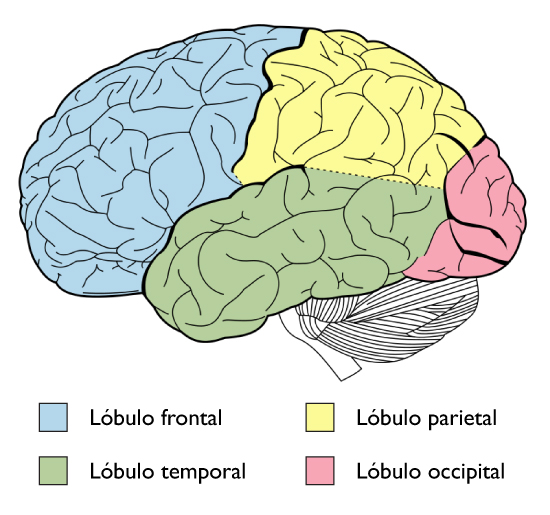
\includegraphics[scale=0.5]{images/lobulos.jpg}
    %http://www.wikisaber.es/uploadedImages/Recursos/Especial_Cuerpo_Humano/Lobulos_cerebrales.jpg
    \caption{Lóbulos cerebrales}
    \label{fig::lobulos}
  \end{center}
\end{figure}

\begin{itemize}
\item {\bf Lóbulo frontal}\\
Controla la capacidad de movimiento, razonamiento, resolución de problemas, lenguaje y emociones.
\item {\bf Lóbulo parietal}\\
Se encarga de las percepciones sensoriales externas (como manos y pies): sensibilidad, tacto, percepción, presión, temperatura y dolor.
\item {\bf Lóbulo temporal}\\
Se encarga de la audición, equilibrio y coordinación. Recibe y procesa información de los oídos y regula las emociones y motivaciones, como ansiedad, placer e ira.
\item {\bf Lóbulo occipital}\\
Se encarga del procesamiento de la visión y la producción de imágenes.
\end{itemize}

A lo largo de este texto se estudia la composición del cerebro humano en detalle, atendiendo tanto a aspectos arquitecturales como funcionales. Se ha realizado un análisis algo superficial ---sin entrar en detalles muy complejos---, con el único fin de servir como base al presente proyecto. Debe recordarse que el objetivo de este escrito es la elaboración de un sistema informático. No obstante, se han utilizado fuentes ampliamente reconocidas en el campo de la medicina.

El lector se verá sorprendido con pequeñas curiosidades históricas sobre las que se apoyan los conceptos explicados durante el análisis cerebral. El objetivo de las mismas no es otro que facilitar su lectura, ayudando a entender cómo se ha llegado a deducir el funcionamiento de cada área del cerebro.

\subsection{La neuroplasticidad}
\label{sec::neuroplasticidad}\index{neuroplasticidad}

El cerebro humano es un sistema dinámico de redes neuronales con gran potencial de evolución. La plasticidad cerebral, o {\it neuroplasticidad}, es precisamente esa capacidad dinámica que posee el cerebro, que le permite mejorar con el aprendizaje y repetición de ciertos ejercicios, y en la que se basa este proyecto. En la sección \ref{neuroplasticidad} se estudiará en profundidad este concepto, mencionando la evolución de su sensibilidad en base a la evolución del cuerpo humano y comentando algunos estudios interesantes sobre el tema.

Se relacionará la neuroplasticidad con el dolor y estrés crónicos, y se introducirá el interesante concepto del {\it cambio cualitativo}, comparándolo con el entrenamiento por repetición e introduciendo así la idea del entrenamiento cerebral mediante juegos.

\section{El entrenamiento cerebral mediante juegos}

Si hay algo que resulta realmente atractivo para el ser humano es la posibilidad de sobrepasar sus limitaciones, ya sea de forma física ---mediante el deporte--- o de forma mental ---mediante el entrenamiento cerebral---. En este sentido la utilización de pequeños juegos resulta una forma muy amena de hacerlo.

Existen diversos artículos dedicados, total o parcialmente, al estudio del entrenamiento cerebral mediante la práctica de juegos. Algunos artículos, como \cite{Hackley2011}, destacan el éxito de los juegos dedicados al entrenamiento cerebral, como el ``Dr. Kawashima's Brain Training'', de Nintendo. Otros utilizan la mejora obtenida mediante juegos como punto de partida para realizar otros estudios. Un buen ejemplo es \cite{Hirvasoja2004}, donde se estudia el efecto de la práctica de juegos sobre la percepción espacial de los seres humanos, comparando las mejoras obtenidas en función de la edad y el sexo.

La sección \ref{sec::fisiologia} se dedica al estudio del cerebro y desglose del conjunto de habilidades mentales estimulables. Más adelante, en la sección \ref{sec:entrenamiento} se especifica el entrenamiento de esas habilidades mediante los juegos de BreakBrain.

\section{Estructura del documento}

A continuación se ofrece una pequeña descripción del contenido de cada capítulo de este documento:

\begin{definitionlist}

\item [Capítulo \ref{chap:introduccion}: \nameref{chap:introduccion}] Este capítulo sirve como presentación del proyecto, explicando el contexto en el que se enmarca y dando unas primeras pinceladas sobre el desarrollo del mismo.

\item [Capítulo \ref{chap:objetivos}: \nameref{chap:objetivos}] En este capítulo se presentan las motivaciónes que desembocaron en el desarrollo de Breakbrain, así como los objetivos que persigue el mismo, tanto el objetivo general como los diferentes objetivos específicos en los que se desglosa.

\item [Capítulo \ref{chap:antecedentes}: \nameref{chap:antecedentes}] En este capítulo se presenta un análisis sobre el estado del arte en el que se enmarca el proyecto. Se analizarán las tecnologías y herramientas en las que se basa su desarrollo, así como algunos sistemas software precedentes que han servido de inspiración u ofrecen cierta semejanza con el proyecto que nos ocupa. Se presenta además, como pilar fundamental del desarrollo de BreakBrain, un estudio general sobre la anatomía y fisiología cerebral humana.

\item [Capítulo \ref{chap:metodo}: \nameref{chap:metodo}] En este capítulo se explica la metodología seguida durante el desarrollo del sistema informático que supone este proyecto. Se hará un recorrido detallado por todas las etapas del mismo, desde el primer estudio de requisitos hasta la realización de pruebas de diferentes tipos, presentando cada artefacto generado durante el proceso.

\item [Capítulo \ref{chap:arquitectura}: \nameref{chap:arquitectura}] En este capítulo se ofrece una visión detallada de la composición de BreakBrain. Se hará especial hincapié en el despliegue del sistema, los patrones utilizados y la extensibilidad de la plataforma.

\item [Capítulo \ref{chap:resultados}: \nameref{chap:resultados}] En este capítulo se ofrecerá una especificación precisa sobre el entrenamiento cerebral mediante juegos ---para cada una de las áreas mencionadas--- diseñado para BreakBrain.

\item [Capítulo \ref{chap:conclusiones}: \nameref{chap:conclusiones}] En este capítulo se realiza una valoración de los objetivos alcanzados, así como propuestas de futuro y una opinión personal sobre el desarrollo del proyecto.

\item [Anexo \ref{chap::iteraciones}: \nameref{chap::iteraciones}] Este anexo contiene el desglose iterativo del desarrollo de BreakBrain, obtenido a partir de la aplicación del Proceso Unificado de Desarrollo.

\item [Anexo \ref{chap::instalacion}: \nameref{chap::instalacion}] Este anexo muestra el proceso necesario para instalar y ejecutar BreakBrain.

\item [Anexo \ref{chap::guia}: \nameref{chap::guia}] Este anexo ofrece una guía detallada para el desarrollo de juegos para la plataforma.

\item [Anexo \ref{chap::manual}: \nameref{chap::manual}] Este anexo ofrece un manual de usuario para aprender a manejar BreakBrain de una forma sencilla.

\end{definitionlist}


\chapter{Motivación y objetivos}
\label{chap:objetivos}

\drop{E}{n} estos últimos años el ser humano ha ido adquiriendo una cierta preocupación sobre su salud física, lo que está provocando el aumento de la práctica de actividades deportivas de todo tipo con mayor frecuencia que años atrás. Sin duda alguna esto supone un beneficio importante para las personas. Pero la salud física no lo es todo.

En muchas ocasiones las personas no son conscientes de la importancia que tiene para su vida el hecho de mantener una cierta salud mental. Los medios de comunicación de masas no aportan nada a favor de esa concienciación mencionada, de forma que en muchos casos el cerebro es descuidado en cierta manera. Del mismo modo que el entrenamiento físico suele resultar divertido, el entrenamiento mental no tiene por qué no serlo también, a pesar de lo que muchas personas puedan pensar al principio.

¿Y si existe la posibilidad de realizar ejercicio mental de forma amena? Quizá se podría ejercitar la mente inconscientemente o de forma colateral mientras se centra la atención en la práctica de un video juego divertido. ¿Y si puede hacerse de forma social, en colaboración con más personas?

\section{Motivación}

Dada la importancia de la salud ---tanto física como mental--- en la vida de una persona, resulta evidente la necesidad del ejercicio y mantenimiento de la misma. Si la práctica de alguna tarea divertida puede contribuir al objetivo propuesto, obviamente dicha tarea debería ser practicada con frecuencia. Por otro lado, dicha tarea deberá resultar entretenida para que las personas sientan atracción por la práctica de la misma.

Los juegos ocasionales son una buena oportunidad de entretenimiento al alcance de cualquier persona, ya sean ejecutados sobre smartphones, videoconsolas u ordenadores personales. Más concretamente, los juegos multijugador ofrecen una experiencia social adicional. Si existe la posibilidad de combinar el entretenimiento de los juegos ocasionales (tanto monojugador como multijugador) con un cierto entrenamiento cerebral, sin duda será una oportunidad genial para obtener esa salud mental mencionada anteriormente de esa forma divertida de la que se ha hablado.

\subsection{Enfermedad mental}

Con el paso de los años, la ciencia ha permitido prolongar la existencia humana hasta límites que hace sólo un siglo eran insospechados. En España, la esperanza de vida se encuentra alrededor de los ochenta años para los hombres y de los ochenta y cinco para las mujeres. Pero ese incremento de la esperanza de vida también ha destapado enfermedades degenerativas que hace años eran desconocidas ---sirvan como ejemplo el {\it Alzheimer} o la {\it demencia senil}---. Concretamente en España existen en la actualidad un total de ochocientas mil personas a las que se les ha diagnosticado Alzheimer.

Ninguna de las dos enfermedades mencionadas tienen cura a día de hoy, pero eso no es un obstáculo para que se pueda planear una cierta prevención ante las mismas.

\subsection{Prevención de la degeneración neuronal}

Si existe una forma de prevenir ciertas enfermedades mentales propias del envejecimiento humano, y además es susceptible de adaptarse a algún tipo de entretenimiento, nos encontraremos ante una oportunidad expléndida para la mejora de la calidad de vida de las personas de la tercera edad. Quizá exista la posibilidad de reducir considerablemente la probabilidad de padecer una enfermedad mental, ¿por qué no explorarla?

\subsection{Mejora activa}

¿Y si la práctica de una actividad reiterada sirviera de ayuda a esa prevención? Los juegos son un buen ejemplo de actividad a la que las personas se someten voluntariamente con el único propósito de divertirse. Quizá pueda mantenerse ese propósito pero permitiendo además que esos juegos mejoren de alguna forma la capacidad mental del jugador. Si pudiéramos medir esa mejora, cada jugador dispondría de estadísticas evolutivas comparables con las de otros jugadores, y de esta forma se podría someter toda esa recopilación de datos a algún procedimiento de \acf{KDD} para extraer conocimiento, por ejemplo.

\section{Objetivos}
\label{sec::objetivos}

Con la motivación expresada como punto de partida, BreakBrain se presenta con una serie de objetivos bien definidos. A continuación se detallan dichos objetivos, agrupándolos en dos conjuntos principales:

\begin{itemize}
\item {\bf Objetivo general}: A grandes rasgos, qué se pretende conseguir con la realización del sistema informático que supone el proyecto.
\item {\bf Objetivos específicos}: Se trata de una serie de {\it objetivos académicos} ---metas de carácter educativo, destinadas a complementar y ampliar los conocimientos adquiridos durante el estudio de la Ingeniería Informática--- y de unos {\it objetivos funcionales} ---metas específicas de la funcionalidad del producto---.
\end{itemize}

\subsection{Objetivo general}

El objetivo general y detonante motivador para el desarrollo de BreakBrain es la construcción de una plataforma social destinada al entrenamiento de habilidades mentales mediante la práctica de juegos, tanto individualmente como de forma colaborativa y competitiva. La plataforma ofrecerá estadísticas de evolución y permitirá el seguimiento (o suscripción a novedades) de otros usuarios. Así mismo, la plataforma deberá ser extensible, de forma que cualquier desarrollador pueda desarrollar sus propios juegos e integrarlos en el sistema, para que otros usuarios puedan jugar con ellos.

\subsection{Objetivos específicos}

Desde el punto de vista académico, un proyecto tan ambicioso como BreakBrain supone el enfrentamiento del alumno a un problema de gran embergadura, mucho mayor que cualquier otro proyecto que se haya afrontado durante el estudio de la licenciatura de Ingeniería Informática.

Como dice el proverbio árabe:

\begin{quote}
{\it Quien se empeña en pegarle una pedrada a la luna no lo conseguirá, pero terminará sabiendo manejar la honda.}
\end{quote}

Con lo anterior no se pretende insinuar que el desarrollo del presente proyecto se inicie pensando en el fracaso, nada más lejos de la realidad. Lo que se tiene claro desde el primer momento es que el aprendizaje adquirido durante el análisis, diseño e implementación de la plataforma será suficiente motivo como para que merezca la pena un gran esfuerzo, independientemente del grado de éxito que alcance BreakBrain.

Así pues, algunos objetivos académicos y funcionales que se persiguen con este proyecto son los siguientes:

\begin{itemize}
\item Afrontar el desarrollo de una red social desde cero, sin el uso de frameworks especializados, sino contemplando la creación de toda la plataforma paso a paso.
\item Investigar y preveer relaciones entre usuarios. Crear un sistema de recomendación basado en las espectativas de entrenamiento cerebral y resultados de cada usuario.
\item Crear una plataforma extensible mediante un pequeño framework de desarrollo de videojuegos sencillos. El objetivo es que cualquier desarrollador pueda extender la funcionalidad de BreakBrain mediante sus propios juegos.
\item Liderar un proyecto de software libre ambicioso, gestionando la integración de juegos de terceros.
\item Aprender a utilizar correctamente los nuevos estándares de HTML5, CSS3.
\item Afrontar el desarrollo de aplicaciones web de tiempo real mediante el uso de WebSockets.
\item Familiarizarse y ganar experiencia con el lenguaje JavaScript y su uso en el lado del servidor mediante NodeJS.
\item Aprender a utilizar bases de datos documentales no basadas en el lenguaje SQL.
\end{itemize}



% Local Variables:
%   coding: utf-8
%   fill-column: 90
%   mode: flyspell
%   ispell-local-dictionary: "american"
%   mode: latex
%   TeX-master: "main"
% End:

\chapter{Antecedentes}
\label{chap:antecedentes}

\drop{A}{} lo largo de este capítulo se presenta el estudio previo realizado como primer paso a la hora de abordar el proyecto que nos ocupa. En primer lugar se ofrece un análisis de los sistemas software que comparten cierta similitud con BreakBrain (secciones \ref{sec::webs-de-juegos} y \ref{sec::webs-de-brain}), tanto desde el punto de vista de un usuario común como mediante una visión técnica de los mismos. Posteriormente se ofrece un repaso acerca de las tecnologías web más utilizadas y extendidas en la actualidad (sección \ref{sec::desarrollo-web}) para, por último, centrar la atención en el desarrollo de mini-juegos preparados para su ejecución web (sección \ref{sec::desarrollo-juegos}), estudiando las diferentes posibilidades de implementación de los mismos. Como colofón se realiza un estudio de las modernas posibilidades existentes para el desarrollo web de tiempo real.

Mientras que los primeros análisis tratan de resultar amenos a cualquier tipo de lector, las últimas secciones están orientadas a un público con cierto nivel de conocimientos técnicos, dado que supone un paso importante en las decisiones tecnológicas tomadas para abordar el proyecto.

Para finalizar el capítulo se expone un análisis sobre la anatomía y fisiología cerebral humana, atendiendo a los aspectos más importantes para el enrenamiento cerebral ---aspectos que serán explotados por BreakBrain---.

\section{Sitios web de juegos online}
\label{sec::webs-de-juegos}

En la actualidad son cada vez más numerosos los sitios web orientados al ocio. De entre ellos, algunos han ganado popularidad por centrarse en ofrecer multitud de pequeños juegos casuales, sin ninguna finalidad más allá de ofrecer un breve tiempo de diversión. Estos juegos normalmente no constan de una historia larga a la que enfrentarse en varias sesiones de juego, sino que se trata de juegos con unas pocas pantallas o una historia de apenas unos minutos.

Dada la considerable afluencia de público a este tipo de webs, resulta muy común el emplearlas como negocio mediante el uso de la publicidad para proporcionar ingresos, lo que en muchas ocasiones ofrece una experiencia de usuario que deja bastante que desear.

A continuación se ofrece un pequeño análisis sobre algunas de estas webs:

\subsection*{Minijuegos.com}

Con un {\it Pagerank}\footnote{El Pagerank, definido oficialmente como un {\it ``método de asignación de importancia a nodos de una base de datos enlazada''} por \cite{Lawrence2007}, es un algoritmo mediante el cual Google puntúa a cada sitio web según su importancia o influencia en Internet.}\index{pagerank} de 6/10, Minijuegos \cite{Minijuegos} se sitúa a la cabeza de las webs de este tipo. Después de llevar online casi una década, se trata de una muestra clara del crecimiento de Internet y las tendencias que han ido evolucionando a lo largo del tiempo con respecto a las tecnologías utilizadas para la implementación de los juegos (que serán estudiadas en la sección \ref{sec::desarrollo-juegos}).

\begin{figure}[h]
  \begin{center}
    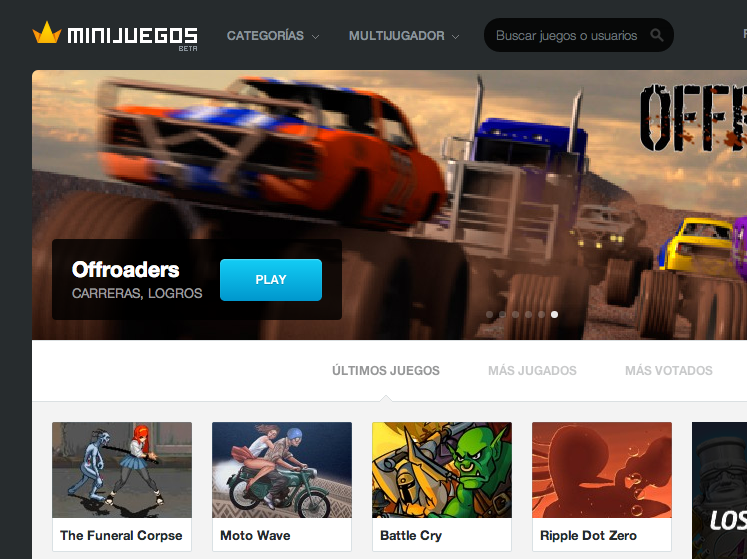
\includegraphics[width=\textwidth]{images/minijuegos.png}
    \caption{Minijuegos\footnote{{\tt http://www.minijuegos.com}}}
  \end{center}
\end{figure}

Su continua renovación, así como su apuesta por un modelo de publicidad poco abusivo, han garantizado su éxito durante años. En la actualidad, ofrecen recursos para que los desarrolladores tengan aún más facilidades para crear sus juegos para la plataforma, soportando varias tecnologías diferentes.

Los juegos de este servicio se clasifican en función de 10 categorías: Acción, Aventuras, Carreras, Clásicos, Deportes, Estrategia, Gestión, Habilidad, Mesa y Colecciones.

Cada una de las categorías contiene entre 5 y 10 subcategorías diferentes, lo que abarca un amplio surtido de juegos de todo tipo. Como último detalle, Minijuegos ofrece además algunos juegos multijugador.

%% \begin{figure}[h]
%%   \begin{center}
%%     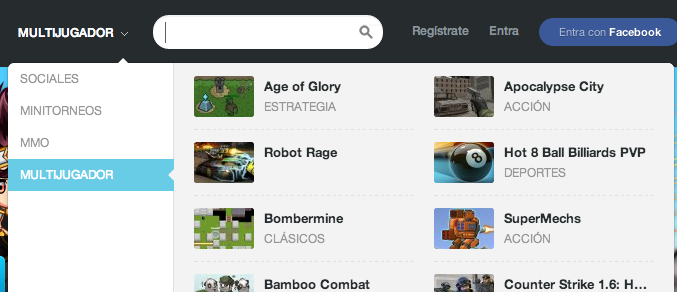
\includegraphics[width=\textwidth]{images/minijuegos-mul.png}
%%     \caption{Juegos multijugador en Minijuegos ({\tt http://www.minijuegos.com})}
%%     \label{fig::minijuegos-mul}
%%   \end{center}
%% \end{figure}

Un punto fuerte de Minijuegos es el conjunto de herramientas y recursos que ofrecen para el desarrollo de juegos por parte de terceros. Ponen \acs{API}s de diferentes tecnologías a disposición de los desarrolladores. Esto garantiza un éxito prolongado de la plataforma, dado que la sencillez de programación de juegos para la misma motiva a los desarrolladores a ampliar su catálogo cada día.

Los juegos están desarrollados en Flash (requieren la instalación de un plugin) y HTML5 (funcionan \acs{OOTB} con cualquier navegador moderno).

\subsection*{Miniclip.com}

Con el mismo pagerank\index{pagerank}, 6/10, Miniclip ofrece también una gran cantidad de juegos, clasificados en más de 70 categorías ---lo cual puede resultar algo abrumador para el usuario---. En la figura \ref{fig::miniclip} se muestra la parte de la interfaz de esta plataforma.

\begin{figure}[h]
  \begin{center}
    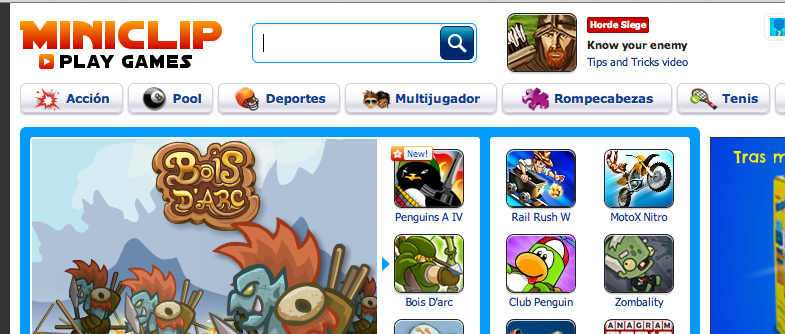
\includegraphics[width=\textwidth]{images/miniclip.png}
    \caption{Miniclip\footnotemark}
    \footnotetext{{\tt http://www.miniclip.com}}
    \label{fig::miniclip}
  \end{center}
\end{figure}

Visualmente, y en cuanto a usabilidad se refiere, Miniclip está muy por detrás de Minijuegos. Además se aprecian pequeños defectos, como el hecho de que exista una categoría llamada {\it Educación} y otra llamada {\it Educativos}, que dan una sensación de una menor profesionalidad.

Los juegos, tanto multijugador como individuales, están desarrollados en Flash y Unity, por lo que requieren la instalación de plugins para poder ser ejecutados.

\subsection*{Minigamesfreak.com}

Bajando bastante el nivel, tanto en cuanto a calidad de la plataforma como a pupularidad, se encuentra Minigamesfreak, con un pagerank\index{pagerank} de 2/10. Se trata de un sitio que recopila juegos individuales de otras plataformas, como Minijuegos. La usabilidad deja mucho que desear, teniendo que pasar por múltiples páginas desde que se hace click sobre un juego hasta llegar a él y poder jugar.

\begin{figure}[h]
  \begin{center}
    
\includegraphics[width=\textwidth]{images/minigamesfreak.png}
    \caption{Minigamesfreak ({\tt http://www.minigamesfreak.com})}
    \label{fig::minigamesfreak}
  \end{center}
\end{figure}

Minigamesfreak tiene un enfoque lucrativo mediante publicidad, algo abusiva, que produce una experiencia de usuario desagradable. Sin prestar ninguna atención al diseño ofrecen una apariencia deficiente y poco atractiva.

\subsection*{Juegosfan.com}

Al igual que Minigamesfreak, Juegosfan ofrece una recopilación de juegos (individuales o monojugador) de otras webs populares, como Minijuegos. No obstante, en este caso se trata de un sitio web más profesional y agradable para el usuario. Con un pagerank\index{pagerank} de 4/10 denota una popularidad importante en Internet.

\begin{figure}[h]
  \begin{center}
    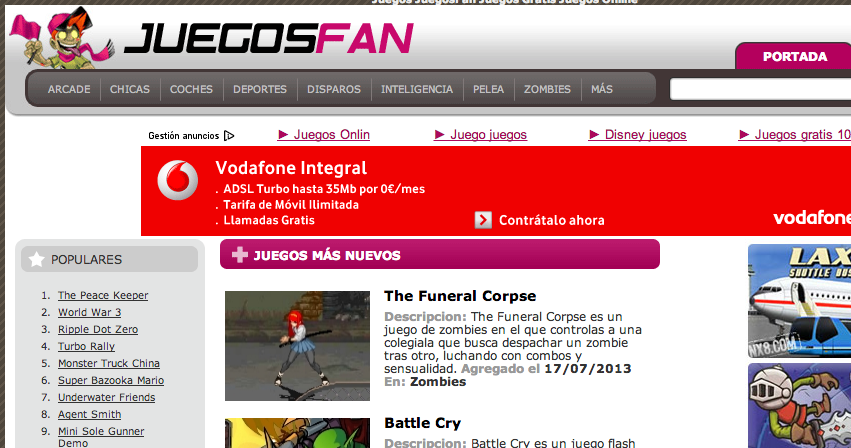
\includegraphics[width=\textwidth]{images/juegosfan.png}
    \caption{Juegosfan ({\tt http://www.juegosfan.com})}
    \label{fig::juegosfan}
  \end{center}
\end{figure}

La interfaz que ofrece está un poco saturada de publicidad, por lo que la experiencia es mejorable.

\subsection*{Minigameonline.net}

De nuevo una web de recopilación de juegos de otras páginas, de un nivel de madurez y popularidad similar al de Minigamesfreak (pagerank\index{pagerank} de 2/10). Con una sencillez mayor, la experiencia de juego mejora frente al primero, dado que cargar cualquier juego es inmediato y no te obliga a pasar por páginas intermedias. Además la publicidad no resulta molesta y queda relegada a un segundo plano.

\begin{figure}[h]
  \begin{center}
    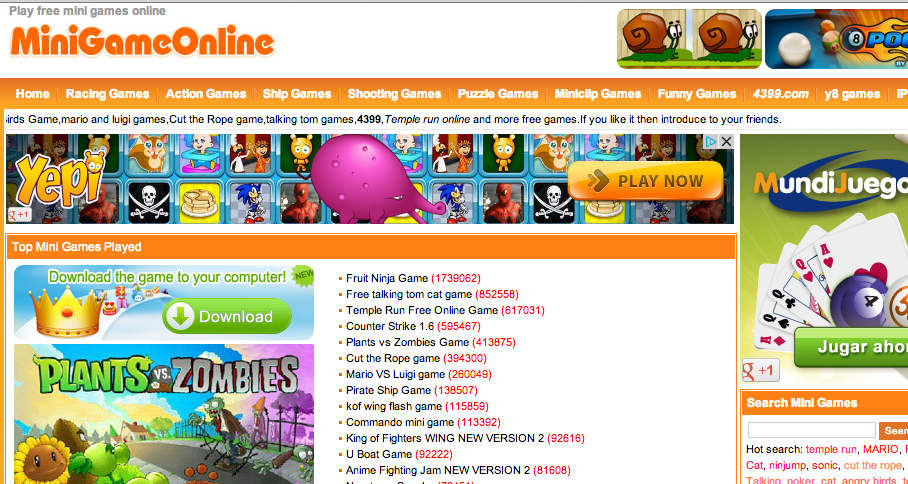
\includegraphics[width=\textwidth]{images/minigameonline.png}
    \caption{Minigameonline ({\tt http://www.minigameonline.net})}
    \label{fig::minigameonline}
  \end{center}
\end{figure}

Los juegos que integra están implementados en Flash, y clasificados en 8 categorías entre las que se incluyen, a parte de las clásicas (Carreras, Acción, Barcos, Disparos, Puzzle...), categorías específicas para las webs de las que se han extraído los juegos, como Miniclip.

\section{Entrenamiento cerebral mediante mini juegos}
\label{sec::webs-de-brain}

En las secciones anteriores han sido expuestas algunas de las plataformas de minijuegos más conocidas de Internet. Se trata de webs recopilatorias de juegos casuales de multitud de temáticas, donde los juegos enfocados al ingenio, la memoria o la educación juegan un papel poco importante ---indistinguible del de juegos de plataformas, carreras, acción, etc---.

En esta sección se analizarán otras plataformas de juegos, esta vez centradas en juegos de estimulación de habilidades mentales.

\subsection*{Lumosity.com}\index{lumosity}

Con un pagerank\index{pagerank} de 6/10, se trata de una de las webs más populares de minijuegos orientados a la estimulación de habilidades mentales. Muestra una interfaz sencilla, con un diseño muy agradable y sin publicidad. La ausencia de anuncios se agradece al utilizar la plataforma, pero tiene un gran inconveniente: el servicio ofrecido es de pago (ver figura \ref{fig::lumosity}). Las tarifas no son demasiado económicas, por lo que emplear la plataforma como entretenimiento casual queda totalmente descartado para la mayoría de usuarios. De forma gratuita no es posible probar ningún juego.

Lumosity está enfocada sobre todo al entrenamiento rutinario, ofreciendo un seguimiento personalizado para cada usuario.

\begin{figure}[h]
  \begin{center}
    
\includegraphics[width=\textwidth]{images/lumosity.png}
    \caption{Lumosity ({\tt http://www.lumosity.com})}
    \label{fig::lumosity}
  \end{center}
\end{figure}

En esta plataforma los juegos son clasificados en 5 categorías: Velocidad, Memoria, Atención, Flexibilidad y Resolución de Problemas. Todos los juegos son individuales ---quedando así anulado cualquier atisbo ``social''--- y están implementados en Flash, con el inconveniente que ello supone: es necesario tener instalado un plugin para esta tecnología.

\subsection*{Brainarena.com}

Con menor popularidad (pagerank de 3/10), Brainarena cambia el enfoque lucrativo hacia un modelo basado en la publicidad, ofreciendo sus servicios de forma totalmente gratuita (como ocurría con las plataformas estudiadas en la sección \ref{sec::webs-de-juegos}) a costa de empeorar considerablemente la experiencia de usuario.

\begin{figure}[h]
  \begin{center}
    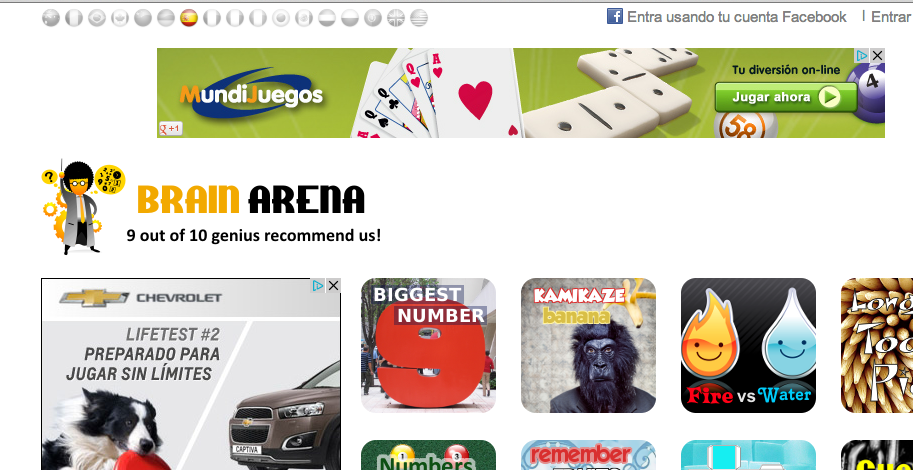
\includegraphics[width=\textwidth]{images/brainarena.png}
    \caption{Brainarena ({\tt http://www.brainarena.com})}
    \label{fig::brainarena}
  \end{center}
\end{figure}


Son sólo 16 juegos los que están al alcance del usuario. La ausencia de categorías para clasificarlos resulta un tanto extraña.

Por otro lado, la jugabilidad es sobresaliente debido a su sencillez: todos los juegos muestran una imagen y dan 4 opciones que pueden ser elegidas con las teclas 1, 2, 3 y 4 del teclado.

\section{Tecnologías Web}
\label{sec::desarrollo-web}

La imparable popularización de Internet ha sido propulsora de una gran evolución tecnológica y social desde que la {\it ``Red de redes''} fue concebida hasta nuestros días. Al principio de la década de los 90 tener un computador personal en casa era un lujo al alcance de pocos, y el acceso a Internet un lujo todavía mayor. Los teléfonos móviles no se empezarían a extender hasta 5 o 10 años después. A día de hoy cualquier persona tiene un ordenador en casa y acceso a Internet. Es más, según \cite{Accenture2012} el 69\% de los accesos a Internet en la actualidad se realizan desde teléfonos móviles.

Internet es una red descentralizada de servicios como \acs{WWW}, \acs{SMTP}, \acs{FTP}, \acs{P2P}, \acs{IRC}, \acs{VoIP}, \acs{SSH}, etc. De entre ellos el de mayor éxito es el primero: la \acf{WWW}, conocida informalmente como {\it ``La Web''}. \acs{WWW} es un conjunto de protocolos que permite la consulta de archivos de hipertexto\index{hipertexto}\footnote{El hipertexto es una herramienta de software con estructura no secuencial que permite crear, agregar, enlazar y compartir información de diversas fuentes por medio de enlaces asociativos. El hipertexto es una de las formas de la {\it hipermedia}\index{hipermedia} ---manipulación de información interactiva en diversos formatos---.}.

La explicación más sencilla del funcionamiento de Internet consiste en la comprensión de dos conceptos: servidor y cliente. Los clientes envían peticiones al servidor, y éste construye y devuelve una respuesta. En el caso de la navegación web, la petición puede ser la solicitud \acs{HTTP}\index{HTTP} \acs{GET}\index{GET} de una página web, y la respuesta el código \acs{HTML}\index{HTML} de la web, que será interpretado y renderizado por el navegador del cliente. Otro ejemplo puede ser una petición \acs{HTTP}\index{HTTP} \acs{POST}\index{POST} de envío de un formulario, y una respuesta de redirección.

A continuación se presentan algunas de las tecnologías web más populares, tanto a nivel del servidor como del cliente.

\subsection{Servidor web}

Un servidor web es un computador que realiza, siguiendo un orden riguroso, las siguientes tareas:

\begin{enumerate}
\item Recibe una petición de un cliente
\item Procesa la petición
\item Realiza la tarea interna correspondiente a esa petición
\item Construye una respuesta
\item Envía la respuesta al cliente que hizo la solicitud
\end{enumerate}

En la actualidad existen numerosas tecnologías y entornos de ejecución para la construcción y despliegue de servidores web, en casi cualquier lenguaje de programación existente. Cada opción tiene sus ventajas e inconvenientes y es más o menos adecuada dependiendo de la situación y finalidad del servidor.

En el caso concreto de las páginas web, el servidor recibe peticiones \acs{GET} y \acs{POST} del navegador web de un cliente y genera código \acs{HTML} y de {\it scripting} (JavaScript) que dicho navegador es capaz de interpretar.

A continuación se exponen algunas de las tecnologías más utilizadas en la creación de servidores web.

\subsubsection{PHP}

PHP\index{PHP} es un lenguaje de {\it scripts} ---scripts del lado del servidor, por lo que no son interpretables por un navegador web cliente--- ampliamente utilizado para todo tipo de propósitos. Está orientado especialmente al desarrollo web, y puede ser empotrado en código \acs{HTML}\index{HTML} (ver listado \ref{code:php}).

\begin{listing}[language=html, caption={Ejemplo de inclusión de código PHP en HTML}, label=code:php]
<!DOCTYPE html>
<html lang="es">
    <head>
        <meta charset="UTF-8" />
        <title> Ejemplo basico PHP</title>
    </head>
    <body>
        <?php
            echo 'Esto es codigo PHP';
        ?>
    </body>
</html>
\end{listing}

Este lenguaje es software libre, y además de ser interpretado por un servidor web también permite su ejecución en un intérprete de comandos común. En \cite{php} se ofrecen recursos útiles para el aprendizaje y primeros pasos del lenguaje.

\subsubsection{ASP.NET}

A diferencia del anterior, éste es un framework diseñado exclusivamente para el desarrollo de páginas web dinámicas y servicios web. Es el sucesor del antiguo \acs{ASP}, lanzado por Microsoft en 1996. Permite su utilización con cualquier lenguaje soportado por el framework .NET (Java, C\#, etc.), y puede ser utilizado únicamente en servidores \acs{IIS} de Microsoft.

En comparación a otras alternativas interpretadas (como PHP), ASP.NET ofrece la ventaja de trabajar con código compilado, lo que le otorga mejor rendimiento.

\subsubsection{JSP (Java Server Pages)}

Aunque Java es un lenguaje de propósito general, no es hasta 1999 cuando Sun Microsystems lanza \acs{JSP} para competir con otros lenguajes y frameworks, PHP y \acs{ASP}.

Esta tecnología requiere una máquina virtual Java, capaz de interpretar su {\it bytecode} \index{bytecode}, y soporta lo que se conocen como anotaciones ---comentarios \acs{HTML} con una sintaxis especial, que permiten la modificación de ciertas partes del código en tiempo de ejecución---.

\subsubsection{NodeJS}

En los últimos años la popularización de JavaScript como lenguaje de programación web (del lado del cliente) ha crecido de forma considerable, ayudada en parte por el desarrollo del motor de ejecución V8 (creado por Google para el navegador Chrome). Lo que no se pensó hasta 2009 era en la posibilidad de utilizarlo en el lado del servidor. Fue entonces cuando Ryan Dahl lanzó NodeJS, un entorno de ejecución de JavaScript nativo, basado en el motor V8, centrado en la entrada salida y basado en eventos.

NodeJS es software libre, está enfocado a la escalabilidad y permite la creación de servidores web de manera realmente sencilla. El listado \ref{nodejs-example} muestra la implementación de un servidor \acs{HTTP} básico que responde ``Hello world''.

\begin{listing}[language=javascript, caption={Servidor web básico implementado con NodeJS}, label=nodejs-example]
var http = require('http');
 
http.createServer(function (request, response) {
    response.writeHead(200, {'Content-Type': 'text/plain'});
    response.end('Hello World\n');
}).listen(8000);
 
console.log('Server running at http://127.0.0.1:8000/');
\end{listing}

La popularidad de NodeJS resulta asombrosa, teniendo en cuenta que se trata de una tecnología muy nueva. En los cuatro años que lleva en desarrollo cuenta ya con más de 37000 módulos registrados en \acs{NPM}, lo que da una idea de la calurosa acogida que ha tenido por parte de la comunidad de desarrolladores.

\subsection{Cliente web}
\label{sec::desarrollo-juegos}

El cliente web es sencillamente un navegador corriente que, principalmente, accede a páginas web y realiza peticiones de formularios. Cuando un usuario accede a una página web, el navegador la solicita al servidor, éste la construye y la devuelve, y el navegador la interpreta y se la muestra al usuario.

Como veremos más adelante, la labor del navegador web va más allá de la mera petición e interpretación de páginas web. Concretamente cuando nos centramos en el desarrollo de videojuegos multijugador, el navegador es también el encargado de mantener la comunicación con el servidor de forma transparente al usuario.

\subsubsection{Tecnologías web para desarrollo de videojuegos}

Existen diversas tecnologías disponibles para la inserción de contenido gráfico animado e interactivo en una página web. A continuación se expondrán las más importantes, absolutas protagonistas del desarrollo de videojuegos web hoy en día.

\begin{itemize}

\item{\bf JApplets}

Durante un largo tiempo, los applets de Java (o JApplets) fueron la fuerza dominante en el desarrollo de contenido interactivo web en el lado del cliente. La popularización de Java como lenguaje de propósito general fue en gran parte la responsable. No obstante, con la modernización de \acs{HTML} y los navegadores web, muchas de las funcionalidades que antes se hacían mediante Java pasaron a estar soportadas \acs{OOTB}, por lo que esta tecnología de Java fue perdiendo popularidad. Nótese que los applets de Java requieren de un complemento adicional o plug-in instalado en el navegador para ser ejecutados.

En la actualidad se utiliza bastante poco, habiendo quedado prácticamente en desuso en el ámbito de los videojuegos (en parte por el bajo rendimiento gráfico que ofrece).

\item{\bf Flash y Shockwave}

Las tecnologías Flash y Shockwave, ambas desarrolladas por Macromedia (empresa que más adelante sería absorbida por Adobe), supusieron una gran evolución en el desarrollo de contenido interactivo web. Hoy en día son ampliamente utilizadas, y ofrecen un rendimiento muy bueno en la reproducción de contenido multimedia ---Shockwave soporta aceleración gráfica---.

Se trata de dos tecnologías complementarias, siendo Shockwave algo más amplia (es capaz de reproducir contenido Flash, lo que no ocurre a la inversa). Requieren de un plug-in para el navegador web. En el caso de Flash, el plug-in se encuentra en el 95\% de los computadores de escritorio, mientras que en el caso de Shockwave sólo en el 40\%, según \cite{w3techs}.

En la actualidad está ocurriendo algo similar a lo que pasó con los applets de Java, y es que \acs{HTML} y los navegadores modernos son capaces de llevar a cabo tareas que antes sólo podía hacer Flash, por lo que cada vez se está empezando a utilizar menos para algunas aplicaciones, debido en parte a la ventaja de no necesitar de plug-ins adicionales.

\item{\bf Unity web player}

Unity es un {\it ``ecosistema de desarrollo de videojuegos''}, según \cite{unity}. Bajo la filosofía \acf{WORE} permite el desarrollo de videojuegos compilables de forma automática para múltiples plataformas. El gran problema de Unity es que es de pago ---con un precio que oscila entre los 1500 y los 6500 euros---, por lo que no se encuentra al alcance de todos los bolsillos.

Entre las ventajas que ofrece frente a otras alternativas, las más importantes son:
\begin{itemize}
\item Rendimiento
\item Calidad gráfica
\item Soporte de plug-ins
\end{itemize}
Unity web player es el componente que permite la ejecución en un navegador de videojuegos creados con Unity. Tal y como ocurría con Flash y Shockwave, si el navegador web no cuenta con el plugin instalado no será capaz de ejecutar el componente.

\item{\bf HTML5}
  
El lenguaje de marcado \acs{HTML} ha ido adaptándose a las necesidades surgidas a causa de la evolución de Internet. En este sentido, la especificación de la última versión (aún no cerrada por completo) incluye funcionalidades que antes eran propias de Flash o los applets de Java, y que ahora cualquier navegador web moderno es capaz de desempeñar. Buen ejemplo de estas funcionalidades son la inclusión de audio y vídeo, así como el objeto {\tt canvas}, que posibilita la creación de videojuegos complejos con un renidmiento excelente.

La tecnología WebGL, parte de la especificación de HTML5, permite incluso utilizar la aceleración gráfica para reproducir contenido 3D de alta calidad. No es de extrañar que HTML5 esté acabando poco a poco con otras tecnologías (que requieren complementos adicionales para ser ejecutadas).

En la figura \ref{fig::webgl} se muestra un ejemplo de la calidad gráfica ofrecida por HTML5. En \cite{chrome-experiments} existe un gran surtido de ejemplos para experimentar con este tipo de contenidos web.

\end{itemize}

\begin{figure}[h]
  \begin{center}
    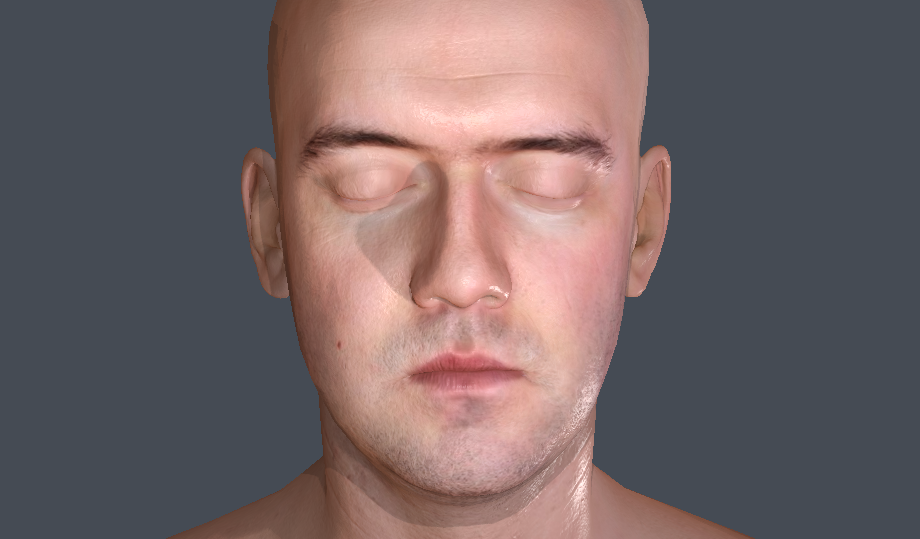
\includegraphics[width=\textwidth]{images/webgl.png}
    \caption{Muestra de las posibilidades gráficas de HTML5 con WebGL}
    \label{fig::webgl}
  \end{center}
\end{figure}

\subsubsection{Comunicación web ininterrumpida: websockets}
\label{sec::tiempo-real}

WebSocket es una tecnología que implementa sockets de comunicación entre servidores y navegadores web (aunque pueden utilizarse por cualquier tipo de aplicación cliente/servidor). Proporciona un canal de comunicación bidireccional y full-duplex sobre un único socket TCP.

Se trata de una tecnología que aún se encuentra en desarrollo. La API de WebSocket está siendo normalizada por el W3C, y el protocolo WebSocket, a su vez, está siendo normalizado por el IETF.

Como las conexiones TCP ordinarias sobre puertos diferentes al 80 suelen ser bloqueadas por los administradores de redes, el uso de esta tecnología proporcionaría una solución mediante la multiplexación de diferentes servicios WebSocket sobre un único puerto TCP.

La especificación del protocolo WebSocket define dos nuevos esquemas de URI:

\begin{itemize}
\item {\tt wss:} para conexiones cifradas
\item {\tt ws:} para conexiones no cifradas
\end{itemize}

El resto de componentes del URI se definen con la sintaxis genérica de URI.

\section{Anatomía y fisiología del cerebro humano}
\label{sec::fisiologia}

% http://www.lumosity.com/knowledge-center/brain-reference/

El primer paso antes de tratar de emplear conocimientos técnicos para mejorar las habilidades mentales de los seres humanos es, evidentemente, la familiarización con la fisiología\footnote{Ciencia biológica que estudia las funciones de los seres orgánicos.} del cerebro, pues de nada sirve tratar de mejorar algo sin conocerlo previamente. En este sentido se ha realizado un esfuerzo adicional por ofrecer esta base científica de una forma amena para el lector. Así pues, en las siguientes secciones se realizará un recorrido por los aspectos más relevantes en cuanto a la estructura y funcionamiento del {\it ``órgano más importante de todos''} \cite{Jacyna2009}.

Una vez adquiridos esos conocimientos previos sobre la materia, nos encontraremos en disposición de diseñar e implementar los mecanismos y métricas más adecuados para la mejora de las funciones cerebrales humanas.

\subsection{Estructura cerebral}

El cerebro de una persona viva es de color rosa, algo pálido. {\it ``Conservado en formol, el cerebro endurece y pierde su color''}, afirma \cite{Czerner2001}. En esta sección hablaremos de las células que constituyen la estructura el cerebro. Estas células se organizan en dos grupos:


\begin{itemize}
\item núcleo\index{núcleo}
\item corteza (o {\it córtex}\footnote{A lo largo de este texto se emplearán indistintamente los términos \emph{corteza} y \emph{córtex}, dado que así se hace en la literatura médica en nuestro idioma.})\index{córtex}
\end{itemize}


\subsubsection{Materia gris, materia blanca y células gliales}

El cerebro es en gran parte de color gris, y es por ello que se emplea la denominación {\it materia gris}. La materia gris está formada por miles de millones de neuronas. Tiene la {\it ``consistencia blanda de harina de avena cocida''}, afirma \cite{Czerner2001}. En la figura \ref{diagrama_neurona} puede apreciarse la forma general de una neurona.


\begin{figure}[h]
  \begin{center}
    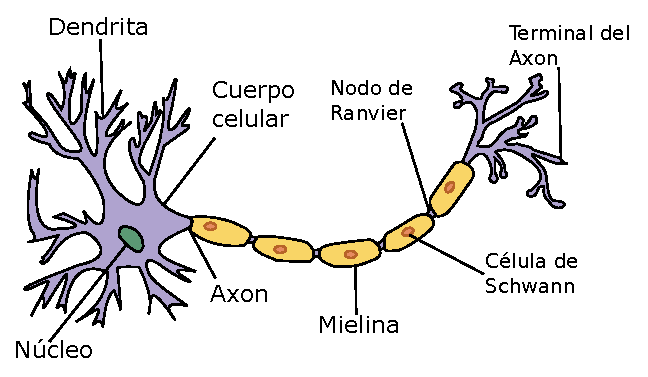
\includegraphics[scale=1]{images/neurona.eps}
    %http://upload.wikimedia.org/wikipedia/commons/6/62/Neurona.svg
    \caption{Diagrama sencillo de una neurona}
    \label{diagrama_neurona}
  \end{center}
\end{figure}


Puesto que hay tantas neuronas, es tentador considerarlas diminutas en términos de su alcance, pero en realidad algunas neuronas tienen axones muy largos. Cuando una multitud de axones se agrupan, aparecen como {\it materia blanca}. En \cite{Czerner2001} se describe la materia blanca como {\it ``una colección de axones largos, aislados, ramas salientes de neuronas que conectan las diversas partes del cerebro entre sí''}, debiendo el color blanco a {\it ``la mielina, un reluciente material aislante que envuelve los largos axones''}.

\cite{Damasio1994} proporciona una descripción sucinta de las materias blanca y gris: {\it ``La materia gris corresponde en gran parte a las colecciones de cuerpos de células nerviosas, mientras que la materia blanca corresponde en gran parte a los axones, o fibras nerviosas, que emanan de los cuerpos celulares en la materia gris''}. Las neuronas se encuentran {\it ``apoyadas por las células gliales''}, que son {\it ``esenciales para la actividad del cerebro''}

Por otro lado, en \cite{Czerner2001} encontramos una buena descripción de las células gliales: {\it ``Cada neurona está rodeado por entre diez y cincuenta células gliales, que constituyen la mayor parte del cerebro. Las células gliales apoyan a la neurona de varias maneras: proporcionan el soporte estructural, aíslan las ramas neuronales con mielina para acelerar la transmisión de señales eléctricas por su axones, mantienen la nutrición de la neurona, ayudan en la eliminación de residuos, e incluso establecen los marcadores que conducen las ramas de una neurona en desarrollo a su destino correcto''}. Como detalle curioso, en el mismo libro se afirma que {\it ``un estudio del cerebro de Albert Einstein demostró que es posible que tuviera un exceso de células gliales''}.

\subsubsection{Cortezas y núcleos cerebrales}

{\it ``La materia gris se presenta en dos variedades''}, afirma \cite{Damasio1994}. {\it ``La primera variedad de materia gris es la formada neuronas que se colocan en capas, como en una torta, para formar una corteza. Ejemplos son la corteza cerebral que cubre los hemisferios cerebrales y la corteza cerebelosa que envuelve el cerebelo. En la segunda variedad de materia gris, las neuronas no están estratificadas, sino que se organizan como cacahuetes dentro de un tarro de cristal. Esta formación constituye un núcleo''}.

\index{neocórtex}

El mejor ejemplo de neuronas organizadas en forma de corteza es la {\it neocorteza} o {\it neocórtex}, a menudo llamada {\it corteza cerebral}. El neocórtex se pliega de una manera que permite a una superficie más grande encajar dentro de los confines del cráneo humano. Los anatomistas llamar {\it surcos} a los pliegues corticales, y {\it giro} a la zona lisa entre dichos pliegues. En la figura \ref{surcosygiros} pueden apreciarse tanto los surcos como los giros de la corteza cerebral.

\begin{figure}[h]
  \begin{center}
    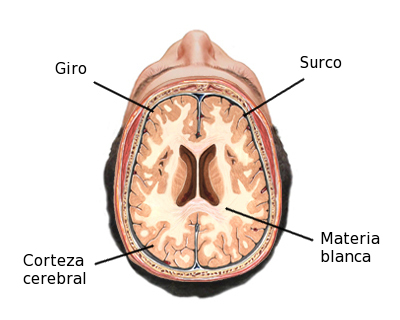
\includegraphics[scale=0.8]{images/surcosygiros.jpg}
    %http://nymethodist.adam.com/graphics/images/en/19238.jpg
    \caption{Surcos y giros del cerebro humano}
    \label{surcosygiros}
  \end{center}
\end{figure}

\subsubsection{Las neuronas}

Los componentes principales de una neurona se detallan en la figura \ref{diagrama_neurona}. La longitud del axón puede ser mucho más larga de como se muestra en la ilustración, tal y como ya se ha dicho cuando se han introducido los conceptos de {\it materia gris} y {\it materia blanca}. Asimismo, en \cite{Sapolsky} se resalta la complejidad de una sola neurona, explicando que puede tener una media de 10.000 dendritas y 10.000 terminales de axón. La comunicación entre las neuronas es tanto química como eléctrica, así que el término electroquímica se utiliza para describir el proceso global.

Simplificando mucho, las moléculas químicas llamadas \index{neurotransmisor} {\it neurotransmisores} son las encargadas de llevar mensajes de una neurona a otra consecutiva. Las vesículas en las terminales del axón de una neurona liberan moléculas de neurotransmisores. Desde un punto de vista químico, una molécula de neurotransmisor {\it ``se ajusta como una llave en una cerradura''}, dice \cite{Sapolsky}, cuando hace contacto con un receptor en las dendritas de una segunda neurona. En \cite{Restak1995} se explica que {\it ``Los receptores son grandes moléculas de proteínas dinámicos que se encuentran a lo largo y dentro de la membrana celular''}. Los receptores pueden, explica el texto, {\it ``verse aumentadas en número y avidez por su neurotransmisor según las circunstancias. Grandes y prolongadas ingestas de ciertas sustancias, por ejemplo, llevar a un aumento en el número de receptores para estas sustancias ---esta es la base de la adicción a las drogas---... Más tarde, si la persona adicta se mantiene alejada de las drogas, los receptores pueden morir''.}

La unión del neurotransmisor y receptor es inhibidora o excitadora. {\it ``Cada neurotransmisor influye en su propio receptor independiente de la acción de los receptores de otros''}, dice \cite{Restak1995}. {\it ``Si bien algunos neurotransmisores pueden disminuir la tensión entre el interior y el exterior de la célula nerviosa y así estimular la célula en acción (neurotransmisor excitador), otras lo aumentan y por lo tanto inhiben la célula de cocción (neurotransmisor inhibidor''}.

Una vez que el \index{neurotransmisor} neurotransmisor y receptor se unen entre sí, \cite{Restak1995} describe su acción como ``dinámica'' y ``exquisitamente sensible''. Hay dos familias de receptores: 

\begin{itemize}

\item {\bf Receptores de canal iónico}

Provocan cambios en la permeabilidad de la membrana y, por lo tanto, regulan el flujo de iones a través de su canal. Cuando un \index{neurotransmisor} neurotransmisor reacciona con su receptor, produce como resultado un cambio en la forma del receptor, de modo que los iones pueden entonces fluir a través de la membrana desde el punto de alta concentración hacia el punto de menor concentración.

\item {\bf Receptores sin canales iónicos}

Actúan a través de intermediarios, las proteínas G, ubicadas en el interior de la célula nerviosa. Básicamente, las proteínas G funcionan como factores de acoplamiento que sirven como enlaces entre el receptor de la superficie exterior de la membrana de la célula nerviosa y un gran número de procesos celulares relacionados entre sí dentro de la célula.

\end{itemize}

Una excitación suficiente en los receptores de los canales iónicos de las espinas dendríticas provoca una onda de cambio iónico que lleva al axón de la neurona a alcanzar su máximo potencial de acción. Una señal eléctrica así desplaza hacia abajo el axón de la neurona y los terminales de los axones para provocar que las vesículas liberen un neurotransmisor químico. En otras palabras, la neurona ``dispara''. Como las vesículas liberan moléculas neurotransmisoras, cada molécula queda ``a la deriva'', con el potencial de hacer contacto con un receptor. Las neuronas, comunicándose entre sí en una dirección, producen un circuito. A menudo existen circuitos alternativos entre las mismas estructuras cerebrales.

Los circuitos neuronales locales en el neocórtex constituyen regiones corticales. Las regiones corticales no solo pueden conectarse unas con otras, sino también con los núcleos subcorticales.

\subsubsection{Neuronas, proyecciones y vías}

\cite{Damasio1994} explica que {\it ``un haz de axones provenientes de fuente conocida y hacia un objetivo determinado se conoce a menudo como proyección, porque proyecta axones a una colección de neuronas. Una secuencia de proyecciones a través de varias estaciones de destino se conoce como vía''}. A menudo se puede ver una vía (materia blanca) a simple vista. Como se ha mencionado antes, \cite{Czerner2001} describe la materia blanca como {\it ``una colección de axones largos, aislados, ramas salientes de neuronas que conectan las diversas partes del cerebro entre sí''}.

% \subsection{El ADN y el comportamiento humano}

% \cite{Brockman} escribe: {\it ``Un gen es un paquete de información, no un objeto o cosa. El patrón de pares de bases en una molécula de ADN especifica el gen, pero la molécula de ADN... es el medio, no el mensaje. Mantener esta distinción entre el medio y el mensaje es absolutamente indispensable para la claridad de pensamiento acerca de la evolución''}.

% A modo de introducción a la genética, hagamos un repaso de abajo a arriba: Existen cuatro compuestos básicos (llamados bases): {\it Citosina}, {\it Adenina}, {\it Timina}, y {\it Guanina}. Estos compuestos se unen entre sí en pares de bases (ver figura \ref{bases}):

% \begin{itemize}
% \item La Adenina (A) se empareja con la Timina (T).
% \item La Citosina (C) se empareja con la Guanina (G). 
% \end{itemize}

% \begin{figure}[h]
%   \begin{center}
%     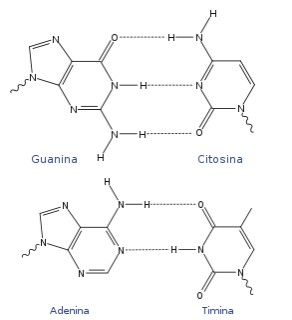
\includegraphics[scale=0.8]{images/bases.jpg}
%     % http://www.forcesystem.com.br/wp-content/uploads/2010/05/adenina-timina-gaunina-citosina.jpg
%     \caption{Pares AT y GC}
%     \label{bases}
%   \end{center}
% \end{figure}

% Estos pares de bases se conectan entre sí para formar dos hélices emparejados, conocidos como {\it ácido desoxirribonucleico (ADN)}. En \cite{JohnAllman2000} se explica cómo se lee el código de pares de bases:

% \begin{quote}
% {\it ``El código de pares de bases se lee en una dirección a lo largo de una hebra. Las secuencias de tres letras (tripletes), especifican cada aminoácido, y las secuencia de tripletes a su vez, especifican la cadena de aminoácidos que forma una proteína. Hay 64 posibles secuencias de tripletes, cada uno codifica uno de los 20 aminoácidos. Así, algunos aminoácidos son especificados por más de un triplete. Los otros tres tripletes son signos de parada que señalan el final de una proteína en concreto. La secuencia completa de tripletes que codifica una proteína es un gen''}.
% \end{quote}

\subsection{El desarrollo cerebral}

Es momento de estudiar el proceso de formación del cerebro humano.


\subsubsection{Introducción a la embriología}
\index{capas germinales}\index{embriología}
En \cite{Shubin2009} se ofrece una genial introducción a lo que se conoce como {\it capas germinales} y a la embriología:


\begin{quote}
{\it ``En la década de 1800, algunos filósofos naturales estudiaron a los embriones para tratar de encontrar el plan común para la vida en la tierra. Uno de estos observadores fue Karl Ernst von Baer, nacido en una familia noble, que inicialmente se formó para ser médico. Su mentor académico sugirió que para tratar de entender cómo funcionan los órganos de un pollo desarrollado, debía estudiar y entender el desarrollo del pollo.

Desafortunadamente, von Baer no podía permitirse el lujo de trabajar en incubadoras de pollos, ni podía permitirse muchos huevos. Por suerte para él, tenía un amigo rico, Christian Pander, que podía darse el lujo de hacer los experimentos. Mientras se fijaban en los embriones, se encontraron con algo fundamental: todos los órganos del pollo se puede remontar a una de las tres capas de tejido del embrión en desarrollo. Estas tres capas se conocían como las capas germinales. Lograron un estatus casi legendario, que conservan aún hoy en día.

El descubrimiento de las tres capas de von Baer dio los medios para hacer preguntas importantes: ¿Todos los animales comparten este patrón? Son el corazón, los pulmones y los músculos de los animales derivados de estas capas? Y, sobre todo, ¿las mismas capas se convierten en los mismos órganos en especies diferentes?

Von Baer comparó las tres capas de embriones de pollo con todo lo demás que pasara por sus manos: peces, reptiles y mamíferos. Efectivamente, pudo concluir que todos y cada uno de los órganos animales se habían originado en una de estas tres capas. Significativamente, las tres capas se formaron con las mismas estructuras en todas las especies. Cada corazón de cada especie estaba formado a partir de la misma capa. Otra capa daba lugar al cerebro de los animales. Y así sucesivamente. No importa lo diferentes que sean las especies, tanto adultos como pequeños embriones, todos pasamos por las mismas etapas de desarrollo''.}

\end{quote}

\subsubsection{Tubo neural}
\label{tubo}
El cerebro comienza a formarse a partir de una estructura en forma de tubo que se conoce como {\it tubo neural}. \cite{Lautin2001} afirma que el comienzo de todo el sistema nervioso central puede ser concebido como un globo inflado, alargado como el que usan los payasos para hacer globoflexia. El tubo neural se flexiona en dos puntos: la {\it flexión cervical} y la {\it flexión cefálica}.

\index{prosencéfalo}\index{mesencéfalo}\index{rombencéfalo}
En las primeras etapas del desarrollo humano, sólo hay tres bultos o vesículas en el tubo neural. A medida que se desarrolla el embrión, estas vesículas comienzan a diferenciarse en subdivisiones que se denominan comúnmente {\it prosencéfalo}, {\it mesencéfalo} y {\it rombencéfalo}. Los seres humanos comparten estas características de desarrollo en el cerebro con todos los demás vertebrados, incluidos los peces vertebrados, los anfibios, los reptiles, las aves y, por supuesto, otros mamíferos.


\begin{figure}[h]
  \begin{center}
    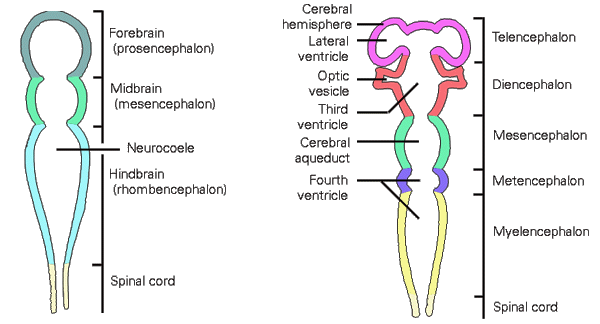
\includegraphics[width=\textwidth]{images/tubo-neural.png}
    % http://www.uoguelph.ca/zoology/devobio/210labs/neuraldevel1.html
    \caption{Tubo neural. A la izquierda el aspecto del tubo en la etapa más temprana de desarrollo, donde pueden apreciarse las 3 partes principales: prosencéfalo, mesencéfalo y rombencéfalo. A la derecha, en una etapa posterior, el prosencéfalo ha pasado a formar el telencéfalo y el diencéfalo.}
    \label{tubo-neural}
  \end{center}
\end{figure}

La figura \ref{tubo-neural} muestra el comienzo de la división del tubo neural. \cite{Lautin2001} señala que, debido a que todo se coloca inicialmente en la línea media, los ventrículos laterales ---una cavidad interna de los hemisferios cerebrales, que serán estudiados en la sección \ref{sec:hemisferios}--- tienen que ser divisiones laterales en los que el tubo neural se vuelve hacia el exterior. En la figura \ref{tubo-neural} se puede apreciar cómo esas divisiones del prosencéfalo comienzan a tomar forma para producir el {\it telencéfalo} (que después evoluciona y forma los hemisferios cerebrales) y el {\it diencéfalo} (que pasa a formar el {\it tálamo} y el {\it hipotálamo}).
\index{telencéfalo}\index{diencéfalo}\index{tálamo}\index{hipotálamo}

En \cite{Lautin2001} se explica que el telencéfalo es ``el ventŕiculo más evolucionado'', una especie de ``cerebro bien formado''. El prefijo {\it tele}, del griego antiguo, significa ``a distancia''. Por otro lado, el prefijo {\it di} de {\it diencéfalo}, según \cite{Lautin2001}, se explica porque el diencéfalo es una especie de ``cerebro de en medio'' o ``inter-cerebro''.


Si bien el \index{mesencéfalo} {\it mesencéfalo} permanece relativamente indiferenciado, el \index{rombencéfalo} {\it rombencéfalo} pasa a formar dos vesículas: la {\it metencéfalo} \index{metencéfalo} (que después pasa a formar el {\it puente troncoencefálico} (o protuberancia anular) y el {\it cerebelo}) y el \index{mielencéfalo} {\it mielencéfalo} (que después se convierte en el {\it bulbo raquídeo}). \index{bulbo raquídeo} \index{puente troncoencefálico} \index{protuberancia anular}

\subsubsection{Integración de neurocircuitos}

A medida que el cerebro se desarrolla, los circuitos neuronales son creados para integrar el cerebro en un todo funcional. \cite{Damasio1994} deja esto claro: {\it ``Hay miles de millones de neuronas en los circuitos de un cerebro humano, el número de sinapsis que se forman entre ellas es al menos de 10 billones, y la longitud de los axones de las neuronas que forman el cableado de los circuitos asciende al orden de cientos de miles de millas. La escala de tiempo para la transferencia de información es muy pequeña, del orden de decenas de milisegundos, lo que significa que en un segundo en la vida de la mente, el cerebro produce millones de patrones de activación sobre una gran variedad de circuitos distribuidos en varias regiones del cerebro''}. Más tarde, el autor añade: {\it ``Los secretos elementales de la mente residen, local y globalmente, en el momento de la interacción neuronal al disparar patrones generados por los circuitos neuronales del cerebro de un organismo vivo''}.

Los desequilibrios en la neurotransmisión de los circuitos cerebrales causan síntomas tales como obsesiones, compulsiones, tics nerviosos y déficit de atención. Algunos factores que influyen en estos desequilibrios son las infecciones virales o bacterianas, incesantes formas de estrés, lesiones físicas, la vulnerabilidad genética, o una combinación de factores. \cite{Damasio1994} afirma que {\it ``La distinción entre enfermedades del cerebro (mente), problemas neurológicos, y problemas psicológicos o psiquiátricos es una desafortunada herencia cultural que permanece en la sociedad, y la medicina refleja una ignorancia básica de la relación entre el cerebro y la mente''}.

\subsection{Estructuras primarias del cerebro}
\label{sec::estructuras-primarias}

{\it ``Debajo de la corteza cerebral, el cerebro humano tiene un parecido sorprendente con los de otras especies mucho más antiguas''}, explica \cite{Czerner2001}. Así como lo hacen en la mayoría de los animales, las neuronas del el bulbo raquídeo y el puente troncoencefálico situado en la base del cerebro, donde nace la médula espinal, de manera constante y fiable regulan sus funciones vegetativas, automatizando su actividad corporal como los latidos del corazón y la respiración. \index{puente troncoencefálico}

\subsubsection{El tronco encefálico. La formación reticular}

El denominado {\it tronco encefálico} (o {\it tallo cerebral}) incluye el \index{mesencéfalo} {\it mesencéfalo} o cerebro medio, \index{puente troncoencefálico} el {\it puente troncoencefálico} y el {\it bulbo raquídeo}. El núcleo del tallo cerebral se llama {\it formación reticular}. La palabra {``reticular''} significa {``red como''}, por lo que dicho núcleo describe el aspecto estructural del tejido del tallo cerebral. Por otro lado, el {\it sistema de activación reticular}, como puede leerse en \cite{Lindberg.}, es {\it ``una parte de la formación reticular que se extiende desde el tronco cerebral hasta el mesencéfalo y el tálamo, con conexiones distribuidas por toda la corteza cerebral y que controla el grado de actividad del sistema nervioso central ---por ejemplo, mantiene el sueño y la vigilia, así como la transición entre los dos estados''}. Existen diversos neurotransmisores implicados en la función reticular del sistema de activación, como la {\it acetilcolina} y \index{acetilcolina}\index{norepinefrina} la {\it norepinefrina}. 

Las neuronas encargadas de la segregación de {\it serotonina}, llamadas \index{núcleos del rafé} {\it núcleos del rafé}, forman una cresta o costura en el centro de la formación reticular. \cite{Panksepp1998} explica que estas neuronas están {\it ``situadas en la línea media del cerebro, lo que indica que son muy antiguas en la evolución del órgano''}. 

En \cite{JohnAllman2000} se señala que {\it ``la red de neuronas serotoninérgicas en el tronco cerebral estaba presente en los primeros vertebrados y ha mantenido una posición anatómica notablemente constante durante la evolución de vertebrados. Las neuronas serotoninérgicas se llaman así porque segregan, desde sus terminales de axón, el neurotransmisor llamado serotonina''}. Más adelante continúa: {\it ``los cuerpos celulares de las neuronas serotoninérgicas ocupan prácticamente la misma ubicación en el interior de cada cerebro de los vertebrados y se encuentran incluso en el mismo lugar en el sistema nervioso central. Este sistema ha sido increíblemente conservado durante la evolución, sin embargo, participa vitalmente en los aspectos más complejos de nuestro pensamiento y de las emociones''}. 

\subsubsection{Generación de patrones}

Aunque rara vez nos detengamos a pensar en ello, nuestro cerebro constantemente genera patrones de actividad, aparentemente sin esfuerzo. Muchos de estos patrones puede continuar incluso después de que ``se apague'' la conciencia. El {\it tallo cerebral} es el ejemplo más obvio de un generador de patrones. En \cite{Shubin2009} se explica lo siguiente: {\it ``Nuestro cerebro puede controlar nuestra respiración sin ningún esfuerzo consciente por nuestra parte. La mayor parte de ese trabajo se lleva a cabo en el tronco cerebral, en el límite entre el cerebro y la médula espinal. El cerebro envía impulsos nerviosos a los músculos respiratorios principales. La respiración sigue un patrón en el que están implicados los músculos del pecho, el diafragma y la garganta, trabajando en un orden bien definido. Por consiguiente, esta parte del tallo cerebral se considera un }generador central de patrones. {\it Esta región puede producir patrones rítmicos nerviosos y, en consecuencia, la activación de los músculos correspondientes. Un número de generadores de este tipo en el cerebro y la médula espinal se encargan del control de otros comportamientos rítmicos, como la ingesta y el caminar''}.

\subsubsection{El sistema nervioso autónomo (SNA)}

Según \cite{Sapolsky2004} "la manera principal en que el cerebro puede decirle al resto del cuerpo lo que debe hacer es el envío de mensajes a través de los nervios que se ramifican desde el cerebro hasta la columna vertebral y hacia la periferia de su cuerpo''. Conocemos mucho el sistema nervioso voluntario, donde {\it ``tú decides mover un músculo y lo mueves''}, dice el autor. Él explica que existe otra parte del sistema nervioso, el {\it sistema nervioso autónomo (\acs{SNA})}, que controla los eventos más espontáneos e involuntarios, tales como el rubor, la {\it piel de gallina}, y el orgasmo.

\cite{Lindberg.} define el SNA como {\it ``una parte del sistema nervioso de los vertebrados que regula las acciones involuntarias''}. Por otro lado, según \cite{MerckCo.} el sistema nervioso autónomo {\it ``funciona automáticamente (de manera autónoma), sin esfuerzo consciente de una persona''} y {\it ``controla los órganos internos, incluyendo los vasos sanguíneos, el estómago, el intestino, el hígado, los riñones, la vejiga, los genitales, los pulmones, los músculos de los ojos, el corazón y el sudor, la saliva y las glándulas digestivas''}.

El \acs{SNA} se compone de dos subsistemas: el {\it sistema nervioso parasimpático} y el {\it sistema nervioso simpático}. La función del sistema nervioso parasimpático es promover la calma, con funciones tales como el descanso y la digestión, mientras que la función del sistema nervioso simpático es la de preparar al indivíduo para luchar o huir. En la figura \ref{fig:sna} se muestra una panorámica fácil de recordar de esta división funcional.

\begin{figure}[h]
  \begin{center}
    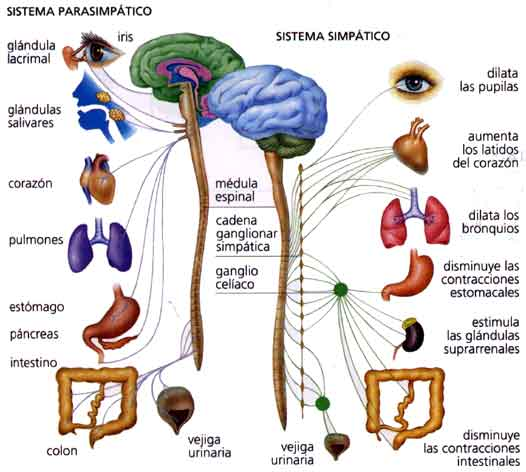
\includegraphics[scale=0.7]{images/sna.jpg}
    % http://lalupa3.webcindario.com/biologia/imagenes/simpatico%20y%20parasimpatico.jpg
    \caption{Subsistemas simpático y parasimpático del SNA}
    \label{fig:sna}
  \end{center}
\end{figure}

\subsubsection{El cerebelo}

\cite{Lindberg.} destaca que el {\it cerebelo} \index{cerebelo} (del latín ``pequeño cerebro'') está {\it ``situado entre el tronco cerebral y la parte posterior del cerebro en los seres humanos, y formado por dos lóbulos laterales y un lóbulo medio''}. En la figura \ref{fig:cerebelo} puede apreciarse la localización del mismo. 


\begin{figure}[h]
  \begin{center}
    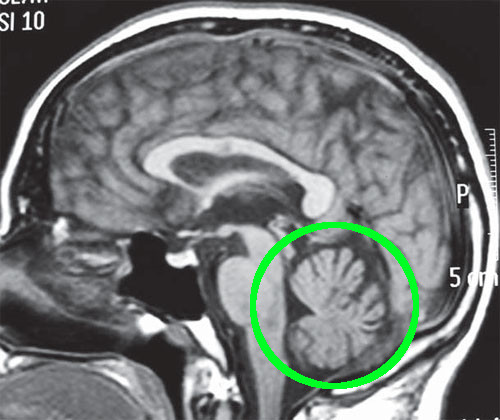
\includegraphics[scale=0.4]{images/cerebelo.jpg}
    % http://www.scielo.cl/fbpe/img/rchnp/v47n3/art07-3.jpg
    \caption{Localización del cerebelo}
    \label{fig:cerebelo}
  \end{center}
\end{figure}

La función principal del cerebelo es la de integrar las vías sensitivas y las vías motoras. Existe una gran cantidad de haces nerviosos que conectan el cerebelo con otras estructuras encefálicas y con la médula espinal. El cerebelo integra toda la información recibida para precisar y controlar las órdenes que la corteza cerebral manda al aparato locomotor a través de las vías motoras. Por ello, lesiones a nivel del cerebelo no suelen causar parálisis pero sí desordenes relacionados con la ejecución de movimientos precisos, mantenimiento del equilibrio, la postura y aprendizaje motor.

Como último detalle, de acuerdo con \cite{MerckCo.} {\it ``hay un creciente consenso en que, además de la coordinación, el cerebelo controla algunos aspectos de la memoria, el aprendizaje y la cognición''}. El texto explica que, aunque la \index{ataxia} {\it ataxia} --- una enfermedad que se caracteriza por provocar la descoordinación en el movimiento de las partes del cuerpo--- es el síntoma más típico de disfunción cerebelosa, muchas otras anomalías motoras también pueden ser fruto de esta disfunción.



\subsection{Los hemisferios cerebrales}
\label{sec:hemisferios}
El cerebro se divide en dos mitades prácticamente simétricas denominadas {\it hemisferios cerebrales} (figura \ref{hemisferios}). En \cite{Restak1994} se analiza cómo los hemisferios izquierdo y derecho responden ante diferentes situaciones, para determinar la funcionalidad de cada uno:

\begin{quote}
{\it ``El hemisferio derecho es dominante para cuestiones no verbales, tareas espaciales, interpretación de gestos faciales y emociones, visualización y transformación mental, y para la apreciación e intuición de figuras geométricas. Por otro lado, el hemisferio izquierdo se centra en el habla, la escritura y la comprensión oral, así como el cálculo.\\
Pero aún más importante que la división funcional es el hecho de que cada hemisferio tiene su propia consciencia.''}
\end{quote}

Ambos hemisferios funcionan de forma diferente al procesar emociones. Mientras que el hemisferio derecho responde ante emociones negativas, el izquierdo lo hace ante emociones positivas. Cuando el hemisferio derecho sufre daños, en \cite{Panksepp1998} se explica que {\it ``con frecuencia los pacientes permanecen alegres, pese a la gravedad de sus problemas''}. Por otro lado, un daño similar en el hemisferio izquierdo {\it ``puede causar estrés emocional catastrófico, predisponiendo a los pacientes a sufrir depresión''}.

\begin{figure}[h]
  \begin{center}
    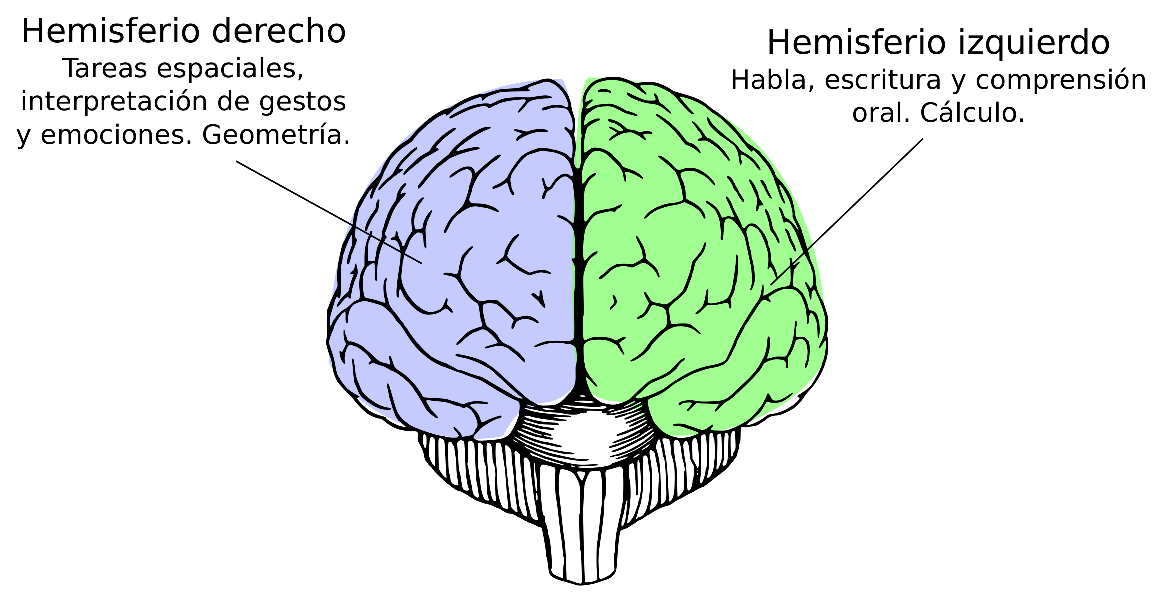
\includegraphics[width=10cm]{images/brain2.eps}
    \caption{Hemisferios cerebrales (vista frontal)}
    \label{hemisferios}
  \end{center}
\end{figure}


\subsection{La corteza cerebral}
\label{sec::corteza-cerebral}

\cite{JohnAllman2000} define ``córtex'' como {\it ``la cubierta externa o corteza de un objeto''}.

\subsubsection{El neocórtex}
\index{neocórtex}
\index{prosencéfalo}\index{mesencéfalo}\index{rombencéfalo}
Como se mencionó en la sección \ref{tubo} cuando se describía el desarrollo del tubo neural, el {\it prosencéfalo} (cerebro anterior), el {\it mesencéfalo} (cerebro medio), y el {\it rombencéfalo} (cerebro posterior) son las partes del cerebro humano durante el comienzo del desarrollo del sistema nervioso central. Durante el desarrollo embrionario el prosencéfalo se divide en {\it diencéfalo} (tálamo e hipotálamo), y {\it telencéfalo} (hemisferios cerebrales).

{\it ''El neocórtex\footnote{También conocido como {\it neocorteza} en la literatura médica española.} es una especialización en el telencéfalo que es paralelo a la formación de la cresta dorsal ventricular en reptiles y aves. El neocórtex es tanto una característica única de mamíferos como son las glándulas mamarias o el martillo y el yunque en el oído medio''}, según \cite{JohnAllman2000}, y {\it ``almacena información acerca de la estructura del medio ambiente a fin de que el mamífero puede fácilmente encontrar alimentos y otros recursos necesarios para su supervivencia''}.

Por otro lado, \cite{Sapolsky} se refiere al {\it neocórtex} como una {\it ``especialización primate''}, terminología que corresponde con la descripción anterior.

\subsubsection{La corteza del cíngulo anterior: emoción, atención y memoria a corto plazo}

Antes de discutir las diferenciaciones anatómicas denominadas lóbulos conviene hablar de la corteza del cíngulo anterior, una zona importante de la corteza cerebral que tradicionalmente se ha considerado parte del sistema límbico\index{sistema límbico}\footnote{Sistema formado por varias estructuras cerebrales que gestionan respuestas fisiológicas ante estímulos emocionales. Está relacionado con la memoria, la atención, los instintos sexuales, las emociones ---placer, miedo, agresividad---, la personalidad y la conducta.}. Desde el punto de vista evolutivo, cabe destacar que la corteza del cíngulo anterior es más antigua que las zonas exteriores de la corteza.


\begin{figure}[h]
  \begin{center}
    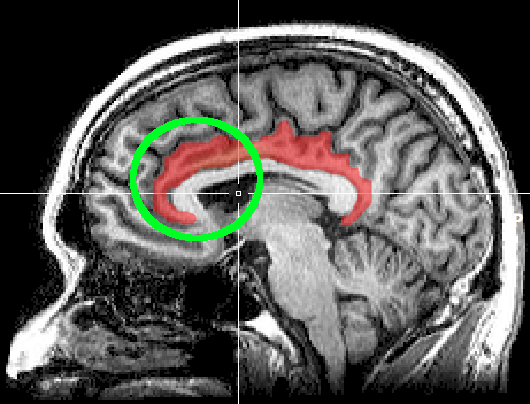
\includegraphics[scale=0.5]{images/cingulo.png}
    \caption{Corteza del cíngulo anterior}
    \label{cingulo}
    % http://upload.wikimedia.org/wikipedia/commons/7/7f/MRI_cingulate_cortex.png
  \end{center}
\end{figure}

La corteza del cíngulo anterior se amolda a la curva exterior del cuerpo calloso, la gruesa banda de fibras nerviosas que conecta los hemisferios izquierdo y derecho del cerebro (ver hemisferios en figura \ref{hemisferios}). El término ``cíngulo'' proviene del latín, y significa cinturón o faja. Este área también es denominada {\it circunvolución cingulada}. \cite{Lindberg.} define ``anterior'' como  {\it ``en relación con o que se encuentra cerca o hacia la cabeza...''}. En la figura \ref{cingulo} la corteza del cíngulo (tanto anterior como posterior) se muestra resaltada, mientras que la parte anterior se encuentra, además, rodeada.

En \cite{Damasio1994} el autor escribe: {\it ``Me gustaría proponer que existe una región particular del cerebro humano donde los sistemas afectados por la emoción / sentimiento, la atención, y la memoria a corto plazo interactúan tan íntimamente que constituyen la fuente de la energía de la acción exterior (movimiento) y la acción interna (pensamiento animación, razonamiento). Esta región manantial es la corteza cingulada anterior, otra pieza del rompecabezas que constituye el sistema límbico\index{sistema límbico}''}. Después continúa diciendo: {\it ``Mi idea acerca de esta región proviene de la observación de un grupo de pacientes con daño en y alrededor de ella. La enfermedad se describe mejor como animación suspendida, mental y externa ---la variedad extrema de un deterioro del razonamiento y de expresión emocional---.''}.

Lo anterior llama la atención sobre un fenómeno interesante que ilustra la función de la corteza cingulada anterior. {\it ``Cuando una apoplejía destruye la corteza motora en el hemisferio izquierdo del cerebro y, como resultado, el paciente tiene parálisis en el lado derecho de la cara''}, comenta \cite{Damasio1994}, {\it ``los músculos no pueden actuar y la boca tiende a ser arrastrada hacia un lado al pedirle al paciente que la abra --- los dientes revelan un aumento de la asimetría---. Sin embargo, cuando el paciente sonríe o se ríe espontáneamente, en respuesta a una observación humorística, sucede algo completamente diferente: la sonrisa es normal, los dos lados de la cara se mueven de forma correcta, y la expresión es natural, nada diferente de la sonrisa habitual pre-parálisis de esa persona. Esto pone de manifiesto que el control motor para una secuencia de movimientos relacionada con las emociones no se encuentra en la misma ubicación que el control de un acto voluntario. El movimiento relacionado con las emociones se desencadena en otras zonas del cerebro, incluso si los músculos objetivos del movimiento son los mismos.''}

Para aclarar que la expresión emocional tiene su origen, \cite{Damasio1994} escribe: {\it ``Si usted estudia a un paciente en el que un golpe ha dañado la corteza cingulada anterior en el hemisferio izquierdo, verá exactamente el resultado opuesto en reposo o en movimiento relacionado con las emociones, la cara es asimétrica, menos móvil en el lado derecho que en el izquierdo. Pero si el paciente trata de contraer los músculos de la cara deliberadamente, los movimientos se llevan a cabo normalmente y vuelve la simetría. La emoción está relacionada con el movimiento, entonces, se controla desde la región cingulada anterior.''}

La corteza cingulada anterior puede desempeñar un papel importante en los lazos entre padres e hijos.

\subsubsection{Los lóbulos cerebrales}
\label{sec:lobulos}
La diferenciación cerebral en ``lóbulos'' se utiliza para indicar la posición relativa de las estructuras cerebrales. Por ejemplo, la amígdala se encuentra dentro de los lóbulos temporales. Es importante recordar que un lóbulo no funciona independientemente, no son unidades autónomas, sino que son meramente una referencia anatómica. \cite{Damasio1994} señala que {\it ``en un sólo segundo el cerebro produce millones de patrones de activación a través de una gran variedad de circuitos distribuidos en varias regiones del cerebro''}.

Si nos centramos en cualquiera de los hemisferios cerebrales por separado, encontramos una nueva división de funcionalidad: los lóbulos cerebrales (figura \ref{lobulos}):

\begin{figure}[h]
  \begin{center}
    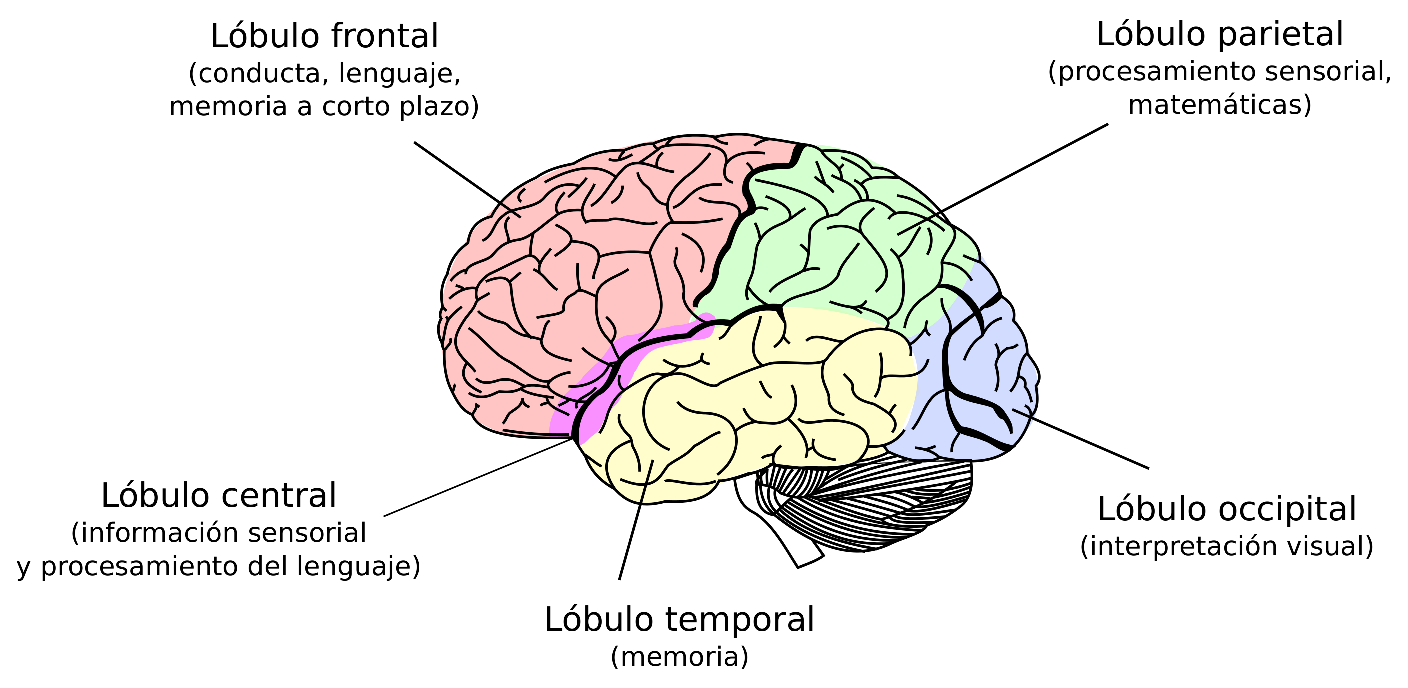
\includegraphics[width=14cm]{images/brain.eps}
    \caption{Lóbulos cerebrales}
    \label{lobulos}
  \end{center}
\end{figure}



\begin{itemize}
\item {\bf Lóbulo frontal}

  Está involucrado en la planificación y priorización de tareas. Según \cite{Restak1995}: {\it ``El lóbulo frontal constituye el 50\% de cada hemisferio cerebral de los seres humanos. Es el encargado de iniciar cualquier actividad motriz, como el habla. Se subdivide en el lóbulo prefrontal ---que integra personalidad con emociones--- y la corteza motora ---que transforma los pensamientos en acciones---.}

\item {\bf Lóbulo temporal}

Contiene un área sensorial relacionada con la audición. Ubicado dentro de cada lóbulo temporal se encuentran la amígdala y el hipocampo, que están, tal como se describe en \cite{Restak1995}, {\it ``implicados en el aprendizaje, la memoria, la experiencia y la expresión de la emoción''}. Una porción del lóbulo temporal, llamada la {\it corteza entorrinal}, conecta las señales corticales de entrada con el hipocampo. {\it ``Las fibras de los cuatro lóbulos, junto con fibras de asociación que unen éstas entre sí, convergen en la región del hipocampo''}, dice \cite{Restak1995}. En \cite{JohnAllman2000} se señala que la amígdala ---tan importante para el procesamiento emocional--- también recibe la entrada de un área cortical en el lóbulo temporal llamada {\it corteza visual inferotemporal}, que es {\it ``más amplia en gran medida en los primates superiores''}. \cite{JohnAllman2000} comenta, además, que {\it ``Charles Goss, Robert Desimone, Rolls Edmund y David Perrett entre otros, han demostrado que las neuronas de la corteza inferotemporal son especialmente sensibles a las imágenes de los rostros''}. \index{córtex/corteza!inferotemporal}


\item {\bf Lóbulo occipital}

Incluye sofisticados mapas topográficos con complejas interconexiones, necesarias para el procesamiento visual y, acorde con \cite{Lindberg.}, tiene {\it ``la forma de una pirámide de 3 lados''}. \cite{MerckCo.} explica que, además de procesar e interpretar la visión, las áreas corticales en el lóbulo occipital permiten al ser humano mantener memorias visuales e integrar percepciones visuales con la información espacial procedente de los lóbulos parietales adyacentes. Si una lesión en la cabeza daña los lóbulos occipitales, en ocasiones se produce lo que se conoce como {\it agnosia visual} ---definida por \cite{MerckCo.} como la {\it ``pérdida de la capacidad de asociar objetos con su habitual papel o función''}---. Con suficiente daño en el lóbulo occipital, {\it ``la gente no puede reconocer caras familiares u objetos comunes, como una cuchara o un lápiz, a pesar de que puede ver estas cosas''}, según se explica en \cite{MerckCo.}.

\item {\bf Lóbulo parietal}

Contiene un área que procesa las sensaciones corporales, llamada {\it corteza somatosensorial}. {\it ``El lóbulo parietal es la estación receptora de la información sensorial desde el lado opuesto del cuerpo y es responsable de la integración de lo que se ve con lo que se siente a través de una red de fibras de asociación''}, explica \cite{Restak1995}.

\item {\bf Lóbulo central o ínsula}

Se encuentra situado {\it ``en el centro del hemisferio cerebral, enterrado entre la unión de los lóbulos frontal y temporal''}, acorde con \cite{Lindberg.}. Según \cite{MerckCo.}, además, la ínsula integra el procesamiento de la información sensorial y autonómica. Involucrado en ciertas funciones del lenguaje, su deterioro puede derivar en la {\it afasia}\index{afasia}, enfermedad que supone la pérdida de capacidad de producir o comprender el lenguaje, tanto hablado como escrito.

\end{itemize}


\subsubsection{La corteza frontal}

\index{neurona!piramidal}

La figura \ref{piramidal} muestra una neurona piramidal, que es común en la corteza prefrontal. La corteza frontal ayuda a centrarse en lo que una tarea es ahora. Los pacientes que sufren demencia en las primeras etapas son incapaces de mantenerse en una tarea concreta, y tienden a volver a tareas anteriores. Sapolsky demostró esta idea con un sencillo experimento consistente en solicitar a pacientes con esta enfermedad que dijeran los meses del año, y después pedirles que contaran hacia atrás a partir 20. El resultado fue que durante la cuenta atrás, los pacientes pasaban a enumerar meses del año, mostrando una imposibilidad para mantener la tarea en la que se encontraban. Esta disfunción se conoce como {\it perseverancia e intrusión} (reversión a una tarea anterior).

\begin{figure}[h]
  \begin{center}
    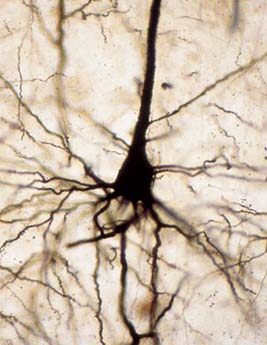
\includegraphics[width=6cm]{images/piramidal.jpg}
    %http://www.kalipedia.com/kalipediamedia/cienciasnaturales/media/200704/17/delavida/20070417klpcnavid_266.Ies.SCO.jpg
    \caption{Neurona piramidal}
    \label{piramidal}
  \end{center}
\end{figure}

{\it ``La corteza frontal está involucrada en el control ejecutivo, sensación de gratificación y planificación a largo plazo''}, explica \cite{Sapolsky2004}. {\it ``Lo hace enviando proyecciones inhibitorias en el sistema límbico\index{sistema límbico}, sistema cerebral involucrado en la emoción y la impulsividad. Además, la corteza frontal resiste entradas estimulantes del sistema límbico\index{sistema límbico}, ignorando tentadores susurros límbicas como \guillemotleft No estudie para el examen, salga a dar una vuelta\guillemotright''}. En el mismo texto se añade que cuando la corteza frontal es destruida, los pacientes sufren deshinibición sexual, agresividad, etc.

Como apunte curioso, en \cite{Johnson2005} se explica cómo si su cerebro se ve dañado en un accidente o derrame cerebral, puede parecer que tiene dañados los lóbulos frontales, incluso cuando los lóbulos frontales permanecen intactos. {\it ``La gente siempre piensa en los lóbulos frontales debido a que son la última estructura en evolucionar, y por lo tanto la más delicada, mientras que las estructuras más antiguas son increíblemente robustas''}. Pero el neuropsicólogo Elkhonon Goldberg, sigue explicando el texto, presentó una teoría diferente: {\it ``Él piensa que, si bien los lóbulos frontales pueden ser más frágiles, hay otro factor en juego, y es que todas las otras partes del cerebro están conectadas a ellos. Al dañar cualquier parte del cerebro, la entrada a los lóbulos frontales se ve alterada, y un cambio en la entrada produce un cambio en la salida. Si los lóbulos frontales no están recibiendo la entrada correcta, es lógico que no produzcan el resultado correcto, aunque estructuralmente estén en perfecto estado. Así que todo el daño cerebral termina pareciéndose a daño en el lóbulo frontal.''}.

{\it ``En los primates, el lóbulo frontal tiene un papel importante en el establecimiento de prioridades y la planificación''}, explica \cite{JohnAllman2000}, {\it ``En particular, la superficie inferior del lóbulo frontal, la denominada corteza orbital-frontal, es especialmente importante para estas funciones''}. La ubicación de la corteza orbital-frontal puede apreciarse en la figura \ref{orbital-frontal}. Cabe destacar que en la literatura médica también se suele utilizar el término {\it región ventromedial del lóbulo frontal} para referirse a la región orbital-frontal.

\begin{figure}[h]
  \begin{center}
    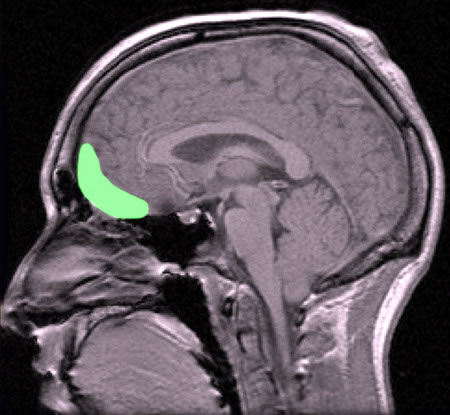
\includegraphics[width=9cm]{images/orbital-frontal.jpg}
    % http://www.blogseitb.com/cienciayhumanismo/wp-content/uploads/2012/10/Orbital-prefrontal-cortex.jpg
    \caption{Corteza orbital-frontal}
    \label{orbital-frontal}
  \end{center}
\end{figure}



\subsubsection{Las áreas de Brodmann}

Según se afirma en \cite{InstituteofNeurosciencesMentalHealth} {\it ``La arquitectura celular difiere suficientemente de una parte del neocórtex a otra como para ser utilizada como un criterio para definir las áreas corticales funcionalmente diferentes''}. Con esa observación, el anatomista alemán Korbinian Brodmann elaboró un mapa de el cerebro basado en las diferencias en la arquitectura celular de las diversas partes de la corteza, asignando a cada parte de la corteza un número del 1 al 52 (ver figura \ref{brodmann}). Respecto a esta división, \cite{InstituteofNeurosciencesMentalHealth} dice: {\it ``La intuición de Brodmann, cuya exactitud ha sido confirmada en muchas ocasiones, afirma que una estructura anatómica particular corresponde a una función en particular. Por ejemplo, el área de Brodmann 17 (que recibe información de un núcleo del tálamo que se conecta a la retina) resulta que corresponde exactamente con la corteza visual primaria.''}. \index{neocórtex}

\begin{figure}[h]
  \begin{center}
    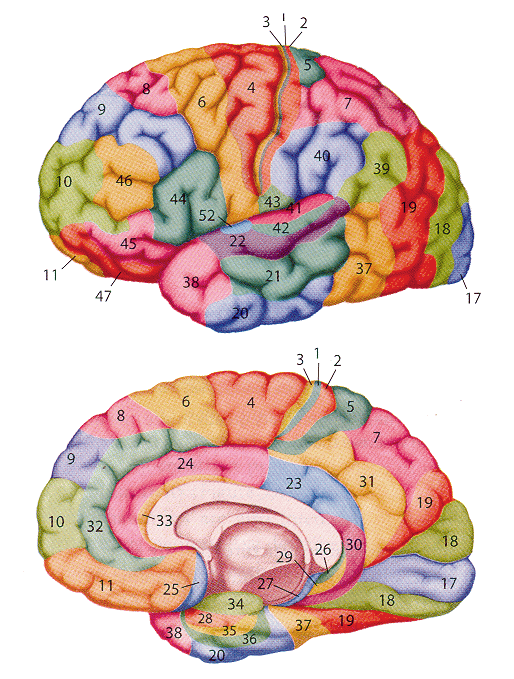
\includegraphics[width=12cm]{images/brodmann-areas.png}
    % http://www.mrc-cbu.cam.ac.uk/people/jessica.grahn/neuroanatomy.html
    \caption{Áreas de Brodmann}
    \label{brodmann}
  \end{center}
\end{figure}


En la figura \ref{brodmann}, {\it la corteza motora primaria} se corresponde con el área 4. El neurocirujano Wilder Penfield Graves (1891-1976) exploró esta región mientras trataba a pacientes con epilepsia severa en Montreal. El objetivo de Penfield era destruir las células nerviosas responsables de la crisis. Mientras el paciente se encontraba bajo el efecto de anestesia local, Penfield estimuló el cerebro con sondas eléctricas, observado las respuestas de los pacientes. Lo hizo para identificar las áreas que requieren cirugía y evitar las áreas vitales que no deben ser destruidas. Al hacer esto, se observó que la estimulación de ciertas áreas de la corteza cerebral desencadenaba contracciones musculares muy localizadas en el lado opuesto del cuerpo. La conclusión fue que las áreas de la corteza asignadas a las diferentes partes del cuerpo {\it ``no son proporcionales a su tamaño, sino más bien a la complejidad de los movimientos que puede realizar. Por lo tanto, las áreas de la mano y cara son especialmente grandes en comparación con las del resto del cuerpo, lo cual no es sorprendente, ya que la velocidad y la destreza de la mano humana y los movimientos de la boca son precisamente los que nos dan dos de nuestras facultades más distintivamente humanas: la capacidad de utilizar las herramientas y la capacidad de hablar.''}.

En \cite{JohnAllman2000} se cita el trabajo de Hughlings Jackson en la determinación de cómo el cerebro controla el movimiento muscular. En la observación de que los pacientes epilépticos en ocasiones sufren crisis convulsivas centradas en un lugar particular en el cuerpo, Jackson {\it ``llegó a la conclusión de que los músculos se representan en el cerebro en un lugar determinado, que dedujo encontrarse en algún lugar de la corteza cerebral o en una estructura cercana llamada cuerpo estriado. Esta teoría fue un cambio radical de la opinión clínica predominante de la época, que era que las crisis epilépticas eran causadas por una alteración en el nivel más bajo del tronco cerebral''}. En el mismo texto puede leerse: {\it ``En 1870, la predicción topográfica de Hughlings Jackson fue confirmada por los médicos alemanes Fritsch y Gustav Eduard Hitzig, quienes descubrieron la corteza motora mediante la estimulación de la superficie del cerebro en perros con débiles corrientes eléctricas y la observación de los movimientos discretos del cuerpo''}. \index{cuerpo estriado}

\index{neocórtex} \cite{JohnAllman2000} explica que las observaciones de Jackson {\it ``se refieren a tres propiedades fundamentales del neocórtex. La primera es que contiene mapas topográficos, la segunda es que las partes más usadas de esos mapas tienen una representación mayor, y la tercera que el neocórtex tiene un papel clave en la génesis de la epilepsia''}. Después continúa diciendo: {\it ``El circuito cortical es muy plástico, ya que puede cambiar su organización funcional en respuesta a la experiencia, y es crucial para la formación de la memoria''}. Esta cualidad plástica del cerebro es la que la literatura médica denomina {\it neuroplasticidad}, concepto que se verá más adelante. \index{neuroplasticidad}

En la figura \ref{brodmann}, las áreas 1, 2 y 3 representan la {\it corteza somatosensorial}, otra especie de mapa topográfico. Si un amigo le hace cosquillas, hay unas zonas muy concretas de la corteza cerebral que se ven activadas. El mapeo somatosensorial permite conocer, monitorizando la actividad cerebral, qué lugar de su cuerpo recibió las cosquillas. En \cite{JohnAllman2000} se explica cómo se descubrieron esos mapas topográficos: {\it ``Con el desarrollo de los amplificadores electrónicos y los osciloscopios de la década de 1930 fue posible registrar la actividad eléctrica de la corteza cerebral. Edgar Douglas Adrian, Woolsey Clinton, entre otros, descubrieron que la región adyacente a la corteza motora se activa eléctricamente por la estimulación mecánica de la superficie del cuerpo; a esa región la llamaron corteza somatosensorial, del griego} soma, {\it que significa} cuerpo. {\it Al registrar actividad en un sitio particular de la corteza somatosensorial, fueron capaces de trazar un campo receptivo en la superficie del cuerpo que activó ese sitio. Con un proceso sistemático encontraron una correspondencia punto a punto en la superficie cortical, por lo que fueron capaces de determinar la representación de la superficie del cuerpo en la corteza somatosensorial''}.

\cite{JohnAllman2000} desarrolla la idea de cómo mediante el uso de grabaciones de microelectrodos, Michael Merzenich, Jon Kaas, y sus colaboradores fueron capaces de confirmar que hay por lo menos cuatro mapas de la superficie del cuerpo en la corteza somatosensorial de los monos. Al igual que los mapas de la corteza motora, los de la corteza somatosensorial en los primates muestran un fuerte énfasis en la mano y la cara, lo que indica la existencia de mayor sensibilidad en las zonas de la mano, los labios y la lengua, que están conectadas a áreas mucho más grandes de la corteza que  las zonas menos sensibles del cuerpo. Al igual que con la corteza motora, los mapas corticales somatosensoriales son plásticos y la representación cortical está más expandida para las partes del cuerpo que son muy usadas. La distinción entre la corteza somatosensorial y la corteza motora no es absoluta. La corteza motora tiene algunas funciones sensoriales y viceversa.

Con respecto al papel de la experiencia en la determinación de las representaciones corticales, \cite{JohnAllman2000} escribe: 

\begin{quote}
  {\it ``Experimentos funcionales realizados en sujetos humanos han demostrado que la representación cerebral de la mano tiene mayor expansión, como resultado de la realización de movimientos complejos de los dedos. La expansión de la representación de la mano puede ser observada tras un corto plazo de capacitación, pero es más notable en los lectores de Braille y en los músicos que tocan instrumentos de cuerda. Estos resultados demuestran el papel de la experiencia: \textit{\textbf{cuanto más fino es el grado de control y el uso de un músculo, mayor será la expansión de su representación en la corteza cerebral}}''}.  
\end{quote}

De nuevo estamos aproximándonos al concepto de {\it neuroplasticidad}, que será desarrollado en la sección \ref{neuroplasticidad}. \index{neuroplasticidad}


\subsubsection{Mapas retinotópicos}

En las áreas del cerebro dedicadas a la vista, los mapas cerebrales son denominados {\it retinotópicos}, puesto que reflejan la topografía de la retina ---la capa de neuronas activadas por la luz que recubren la parte posterior del ojo---. La circuitería visual en la corteza cerebral humana contiene varias docenas de mapas retinotópicos diferentes, cada uno dedicado a analizar el flujo de entrada visual de una forma concreta. La corteza visual primaria ---área 17 de Brodmann (figura \ref{brodmann})--- es el principal receptor de impulsos provenientes de la parte visual del tálamo. Cabe destacar que las áreas visuales además extraen características tales como el color, el movimiento y la forma.

Gran parte del procesamiento visual del cerebro tiene lugar en el lóbulo occipital. Atendiendo a la figura \ref{brodmann}, las áreas dedicadas a esta tarea son la 17, 18, 19, 20 y 21. El área 17 de Brodmann es la corteza visual primaria (V1). El área 18 representa la corteza visual secundaria (V2) y el área 19 la corteza visual asociativa (V3). Cada una de estas áreas constituye un mapa retinotópico. Como se mencionó en el apartado \ref{lobulos}, las áreas de Brodmann 20 y 21 forman parte del lóbulo temporal, y representan la corteza visual inferotemporal, que incluye neuronas sensibles a las imágenes de rostros y envía información visual a la amígdala. \index{córtex/corteza!inferotemporal} \index{córtex/corteza!visual primaria} \index{córtex/corteza!visual secundaria} \index{córtex/corteza!visual asociativa}

En \cite{JohnAllman2000} se detalla cómo la corteza visual primaria (V1) se asignó inicialmente:

\begin{quote}
{\it ``En la guerra entre Rusia y Japón de 1905, muchos soldados japoneses sufrieron heridas de bala en la parte posterior de su cerebro. Debido a la velocidad de salida más alta y el tamaño más pequeño de las balas desarrolladas en el siglo XIX, estas armas tendían a producir lesiones cerebrales más localizadas que las que fueron infringidas en guerras anteriores, lo que mejoró la atención de los heridos y dio lugar a mayores tasas de supervivencia. Muchos de los soldados heridos fueron cegados en parte por estas lesiones, por lo que el oftalmólog Tatsuji Inouye trabajó para el gobierno japonés para evaluar el alcance de su ceguera como un medio para determinar sus beneficios de pensión. Inouye descubrió que la parte del campo visual en el que estos soldados habían quedado ciegos correspondía a la localización de las lesiones cerebrales producidas por los orificios de entrada y salida de la bala. Mediante la combinación del déficit visual de diferentes soldados pudo deducir la organización topográfica de la corteza visual primaria. Inouye reveló que había mucha más corteza dedicada a la representación de la parte central de la retina que a la periferia. Esta es la parte de la retina con mayor agudeza, y es nuestro medio más importante para obtener información del entorno ---y la parte que el lector está empleando en este instante al leer este libro---. El mapa de la corteza visual primaria de Inouye ha sido confirmado por las técnicas modernas de extracción de imágenes cerebrales.''}
\end{quote}

En \cite{Restak1994} se proporciona un ejemplo de cómo el daño a un área del cerebro, en sólo un hemisferio, puede cambiar dramáticamente la forma en que percibimos el mundo. El autor discute cómo Michael Gazzaniga llevó a cabo un experimento que involucró a un sujeto que había perdido la parte izquierda del campo visual a causa de daño cerebral en el área visual del lado derecho de su cerebro: {\it ``Se les pidió que se imaginara a sí mismo mirando hacia California desde Nueva York, y que nombrara los estados que encontraba en medio. Nombró sólo diez estados, todos ellos situados a la derecha de su punto de vista imaginario. Omitió a los estados a la izquierda, que corresponden al campo visual dañado por su lesión cerebral derecha. Lo que no podía ver en el mundo real como resultado de su lesión cerebral, tampoco era capaz de verlo en la imagen espacial de su imaginación''}.

Con el fin de diferenciar la complejidad de las áreas de la corteza visual, en \cite{JohnAllman2000} se citan las diferencias en la corteza visual que distinguen a los primeros mamíferos de los primates y los seres humanos: {\it ``Las zarigüeyas y los erizos, que en muchos aspectos se parecen a los primeros mamíferos que vivieron hace más de 60 millones de años, han limitado su capacidad visual a un pequeño número de las áreas corticales visuales. En los mamíferos, los mapas corticales de la retina son relativamente uniformes en cuanto a la cantidad de espacio cortical dedicado a la parte más central del campo visual, en general en estos animales no es mucho mayor que la corteza dedicada a las partes más periféricas del campo visual. Por el contrario, los primates tienen extremadamente bien desarrolladas las capacidades visuales y tienen un gran número de mapas corticales dedicados a la percepción visual y la memoria. Dentro de la mayoría de estos mapas hay un fuerte énfasis de la representación de la parte central del campo visual y una representación mucho más pequeña de las partes periféricas de la campo visual''}.

\subsection{Estructuras subcorticales. El estrés, las emociones y la enfermedad mental}
\label{sec::estructuras-subcorticales}
% Esta sección es importante. En ella hay un apartado de como el entrenamiento altera el cerebro

En esta sección se estudiarán las principales estructuras subcorticales del cerebro de los mamíferos. En \cite{Panksepp1998}, en referencia al procesamiento emocional instintivo que tiene lugar en nuestras estructuras cerebrales subcorticales, se señala la probabilidad de que, {\it ``en un sentido evolutivo, gran parte del potencial de procesamiento de información en la corteza cerebral es de servicio (se trata de servidores automatizados, a menudo inconscientes) a las instrucciones de los impulsos afectivos que gobernaban el comportamiento previo a la evolución cortical''}.

En \cite{Morrison2009} se ofrece una gran descripción de la similitud entre los humanos y los demás mamíferos. Nosotros, los humanos, compartimos las mismos estructuras cerebrales subcorticales con todos los demás mamíferos. Textualmente:


\begin{quote}

{\it Tanto mi gato Buster como yo nos sobresaltamos y gritamos de dolor ante un estímulo doloroso repentino, y nuestras piernas se contraen en respuesta a un golpe en la rótula de la rodilla. La organización neuronal espinal responsable de estas actividades es la misma, tanto en gatos como en seres humanos.

Profundizando en la parte más baja del cerebro, tanto en Buster como en mí, las mismas neuronas controlan las funciones corporales básicas, tales como la regulación de la respiración, la frecuencia cardíaca y los vómitos. Más hacia adelante residen las células nerviosas que regulan los comportamientos de sueño y la vigilia, que son idénticos en los seres humanos y otros mamíferos, y los resultados de una disfunción en dichas zonas provoca problemas similares, como la narcolepsia \index{narcolepsia} y el trastorno de sueño \acs{REM}. En esta región del cerebro, en todos los mamíferos se encuentran las neuronas que contienen el neurotransmisor dopamina, que degeneran en la enfermedad de Parkinson.

En la base de los hemisferios cerebrales se encuentra la \index{amígdala}amígdala, en forma de almendra, que lidia con el temor y la ansiedad, tanto en personas como animales. Los monos y las ratas han contribuido mucho a nuestra comprensión de la amígdala. La corteza cerebral suprayacente es donde todos nosotros los mamíferos analizamos las sensaciones que provienen de la piel, los músculos y las articulaciones a través de la médula espinal, o los ojos y oídos en el caso de la visión y la audición.

Nos alejamos de otros animales, sin embargo, en el gran desarrollo de la parte delantera de nuestra corteza cerebral, los lóbulos frontales, y la mayor proporción de tejido cerebral, llamadas ``áreas de asociación'', que integran la información obtenida de las regiones que reciben directamente la información sensorial. Estas últimas regiones se llaman las ``áreas primarias sensoriales y motoras'', ya que reciben sensaciones puras y dirigen el movimiento del cuerpo. Se encuentran dentro de los lóbulos frontales, a través de los que nosotros los humanos reflexionamos sobre el pasado y nos preparamos para el futuro. Los animales no tienen esta capacidad última. Los animales se prepararse para el futuro de una forma limitada ---por ejemplo, la ardilla piensa en recolectar y enterrar nueces para el invierno---.}

\end{quote}


\subsubsection{El cerebro animal}

En \cite{Johnson2005} se relata el primer encuentro del autor con con el tejido cerebral real. {\it ``El cerebro de cerdo fue un gran shock para mí porque cuando comparamos las estructuras de nivel inferior, como la amígdala, a las mismas estructuras en el cerebro humano no podía ver ninguna diferencia en absoluto. El cerebro de cerdo y el cerebro humano se veían exactamente idénticos. Pero cuando miré a la neocorteza, la diferencia fue enorme. el neocórtex humano es visiblemente más grande y doblado hacia arriba, y cualquiera puede verlo sin necesidad de un microscopio''}.


\begin{figure}[h]
  \begin{center}
    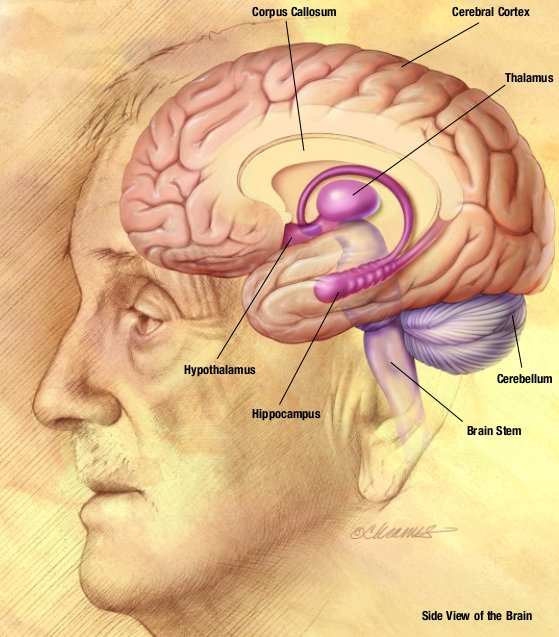
\includegraphics[width=10cm]{images/amigdala.jpg}
    % http://www.neurosciencerus.org/wyHumanBrain.jpg
    \caption{Hipotálamo. Tálamo. Hipocampo. Cerebelo. Cuerpo calloso. Neocórtex. Tallo cerebral}
    \label{fig:amigdala}
  \end{center}
\end{figure}

En la figura \ref{fig:amigdala} se muestra la {\it amígdala}\index{amígdala}, el {\it hipocampo}\index{hipocampo} y el {\it cuerpo calloso}\index{cuerpo calloso}. Debe recordarse que los hemisferios izquierdo y derecho contienen cada una de estas estructuras, que son imágenes especulares el uno de otro.

\subsubsection{La amígdala, el estrés, el \acs{TOC} y el \acs{TEPT}}

\cite{Czerner2001} describe la {\it amígdala}\index{amígdala} como una estructura ``almendrada''. La amígdala se encuentra protegida dentro de cada lóbulo temporal. El lóbulo temporal se encuentra detrás de los templos\index{templo}, de ahí su nombre.

En \cite{Damasio1994} se explica que {\it ``el primer indicio de la relación existente entre la amígdala y las emociones se pueden encontrar en la obra de Heinrich Klüver y Paul Bucy, quienes demostraron que la extirpación quirúrgica de la parte del lóbulo temporal que contiene a la amígdala provoca indiferencia afectiva, entre otros síntomas''}.

Diversas investigaciones demuestran que si la {\it amígdala}\index{amígdala} está dañada, el ser humano pierde la capacidad de discernir las emociones, especialmente el miedo y la ira. Según \cite{JohnAllman2000}, el papel de la amígdala en la percepción de las expresiones faciales {\it ``se mostró claramente en los trabajos de Ralph Adolphs''}. Ralph Adolphs estudió a un paciente que había sufrido un daño bilateral amigdalar sin lesiones significativas en otras partes del cerebro. Aunque este paciente tenía una visión normal y podía percibir rostros, no era capaz de discriminar el contenido emocional de las expresiones faciales negativas del miedo y la ira. Así, todos los rostros le parecían estar sonriendo o mostrando una expresión neutral, incluso los que mostraban un gesto exagerado. El daño a la amígdala\index{amígdala} también afecta a la capacidad para discernir la emoción en el habla. {\it ``Sophie Scott y sus colegas encontraron que la lesión amigdalar también afecta a la capacidad de percibir el contenido emocional de la entonación del habla, a pesar de que su paciente tenía una audición normal. Al igual que con las expresiones faciales en pacientes de Adolphs, las expresiones auditivas del miedo y la ira fueron las más confundidas''}.

El hipocampo y la corteza prefrontal\index{córtex/corteza!prefrontal} se ven reducidos por el estrés, según afirma \cite{Pittenger2008}, mientras que la amígdala\index{amígdala} ve incrementado su tamaño y potenciado su funcionamiento, lo que le permite ser más poderosa con el tiempo ---incluso llegando a ejercer control sobre nuestro razonamiento---. Dicha actividad potenciada puede exacerbar los síntomas de la enfermedad mental, incluyendo el \acs{TOC}.

En \cite{Sapolsky2004} se hace hincapié en que si bien los {\it glucocorticoides}\index{glucorticoides}\footnote{Los {\it glucorticoides} son hormonas de acción contraria a la de la {\it insulina}\index{insulina} en sangre. También actúan sobre el metabolismo intermedio de grasas y proteínas. Los {\it glucocorticoides} producidos por el cuerpo humano son el {\it cortisol}\index{cortisol}, la {\it cortisona}\index{cortisona} y la {\it corticosterona}\index{corticosterona}.} liberados durante episodios de estrés pueden alterar la función del hipocampo y la memoria, los {\it glucocorticoides} mismos incrementan la excitabilidad de la {\it amígdala}\index{amígdala}, permitiendo que las neuronas crezcan más allá de la simple unión entre células.


Especialmente en relación con el \acs{TEPT}, la experiencia es un factor clave. Los neurocientíficos han descubierto que la experiencia moldea la {\it amígdala}\index{amígdala}. Se podría decir que la {\it amígdala} ``aprende'', con el tiempo, el nivel de peligro que debe ser asociado a cada estímulo en particular. En la definición de relevancia incentivo, los autores Vilayanur S. Ramachandran y Lindsay M. Oberman expertos describen el proceso por el cual amígdala puede predecir el peligro. Según \cite{Oberman2006}:

\begin{quote}
{\it ``Cuando una persona ve el mundo, él o ella se enfrenta a una enorme cantidad de información sensorial ---sonidos, olores, etc.---. Después de ser procesada en las áreas sensoriales del cerebro, la información es transmitida a la amígdala\index{amígdala}, que actúa como un portal para el sistema límbico\index{sistema límbico}. La amígdala\index{amígdala} determina la forma en que la persona debe responder emocionalmente: con el miedo (a la vista de un ladrón), la lujuria (al ver a un amante) o indiferencia (cuando se enfrentan a algo trivial). La amígdala envía mensajes al resto del sistema límbico\index{sistema límbico} y, finalmente, alcanza el sistema nervioso autónomo, que prepara al cuerpo para la acción. Si la persona se enfrenta a un ladrón, por ejemplo, su ritmo cardíaco aumenta y su cuerpo comienza a sudar para disipar el calor generado por el esfuerzo muscular. La activación autonómica, a su vez, alimenta al cerebro con información de vuelta, amplificando la respuesta emocional. Con el tiempo, la amígdala\index{amígdala} crea un mapa que detalla el significado emocional de todo en el ambiente del individuo''}.
\end{quote}

En \cite{LeDoux1996} se ofrece un extracto de un informe de Heinrich Klüver y Paul Bucy sobre el comportamiento de un mono tras la extirpación de sus lóbulos temporales ---donde se encuentra la {\it amígdala}\index{amígdala}---. Dicho informe explica cómo el mono no muestra ira ni miedo, y parece incapaz de reconocer objetos:

\begin{quote}
{\it ``El animal, estando hambriento y siendo enfrentado a una variedad de objetos ---un peine, una perilla de baquelita, una semilla de girasol, un tornillo, un palo, un trozo de manzana, una serpiente viva, una pieza de plátano, y una rata viva---, los recoge indiscriminadamente. Lleva cada objeto a la boca, y lo deshecha si no es comestible''}.
\end{quote}

Klüver y Bucy se refieren a este conjunto de síntomas como {\it ``ceguera psíquica''}, dado que los animales tenían una agudeza visual perfecta, pero eran ciegos a la importancia psicológica de los estímulos. Además, \cite{LeDoux1996} explica cómo después de la eliminación de los lóbulos temporales, los monos se convirtieron en {\it ``hipersexuales''}, tratando de copular con otros monos del mismo sexo o con los miembros de otras especies (actividad sexuales rara vez practicada por ``monos normales'').


\subsubsection{Cómo la experiencia afecta al cerebro}

¿Es posible que el entrenamiento pueda crear conexiones neuronales capaces de automatizar comportamientos instintivos? En \cite{Sapolsky} se examina cómo la comunicación entre las neuronas se ve fortalecida como resultado de la experiencia. Sin duda alguna, este punto es clave en el desarrollo de este proyecto, puesto que su pilar fundamental es la posibilidad de mejorar las habilidades mentales mediante cierto tipo de entrenamiento.

Cuando los terminales de las dendritas de las neuronas se estimulan de forma rápida, la comunicación entre las neuronas se ve potenciada {\it ``potenciada''} por ciertos cambios químicos producidos en el contexto neural. Posteriormente, se necesita una menor estimulación para provocar ese mismo nivel de activación neuronal. Esto es así debido a que en el momento en que se percibe una señal eléctrica a través del axón de la neurona, se produce la liberación de los mensajeros químicos llamados {\it neurotransmisores} \index{neurotransmisor} en la sinapsis entre las neuronas, lo que a menudo aumenta la probabilidad de que otras neuronas se dispararen en un especie de reacción en cadena. En otras palabras, el autor afirma que la potencia de activación neuronal se incrementa. Esa potenciación en un tiempo largo es lo que se conoce como {\it ``potenciación a largo plazo''}, y constituye la base para el aprendizaje y la memoria, posiblemente incluso de las formas perjudiciales de aprendizaje, tales como el trastorno de estrés post-traumático (TEPT).

%{\it ``La activación neuronal reconecta el cerebro... anatómicamente el cerebro se forma de nuevo en respuesta a pequeños estímulos nocivos... La activación parece ser un tipo de aprendizaje, pero un aprendizaje que puede ocurrir independientemente de la cognición... la enfermedad, una vez diagnosticada, puede llegar a ser sensible a los estímulos cada vez más pequeños y, con el tiempo, completamente independiente de ellos. El trastorno se vuelve más complejo con el tiempo''}, cita \cite{Kramer1997}.

En \cite{MacLean} el autor teoriza sobre el proceso de activación neuronal: {\it ``Es posible que si un cierto patrón eléctrico de información fuera repetido durante un período prolongado de tiempo, o a intervalos repetidos, en el circuito neuronal, las células nerviosas se sensibilizaran de forma permanente a responder a este patrón particular en algún momento futuro. Tal mecanismo proporciona una variedad de memoria perdurable.''}.

Citando textualmente a \cite{Gallagher}:

\begin{quote}  
{\it Con el tiempo, repetidas experiencias estresantes pueden, literalmente, y no sólo en sentido figurado, alterar el sistema nervioso de las personas. La investigación en animales ha demostrado que cuando a una rata se le da una pequeña descarga no muestra ninguna reacción notable, pero al ser expuesta a factores de estrés tales como la repetición de descargas durante cinco días consecutivos, muestra signos de respuesta al estrés, cuando se expone durante siete u ocho días, la rata tiene un ataque, y a partir de entonces se mantiene alterada y ataca con poca o ninguna provocación. Experimentos de este tipo, por supuesto, no se llevan a cabo con personas, pero Philip Gold y otros neurocientíficos piensan ahora que en los seres humanos, también mediante la activación de una cascada de reacciones químicas, puede producirse un estrés crónico grave, sobre todo en los primeros años de vida, y causar cambios en los genes de manera que se altere la funcionalidad de las células del cerebro de forma permanente. Debido a que las neuronas requieren un tipo particular de entrada para activarse o desactivarse, sólo algunos miles de neuronas, cada una de las cuales está implicado en algún aspecto de la estructura celular o de comunicación, se activan en un momento dado. Cuando una persona de temperamento vulnerable es constantemente bombardeados con estímulos perturbadores, dice Gold, los genes que se activan son los que participan en los componentes celulares de la respuesta al estrés.}
\end{quote}

La neurotransmisión en la amígdala a veces es activada para generar comportamientos impulsados por la {\it dopamina}\index{dopamina}, como conductas orientadas a resolver problemas de control corporal y de confianza. En circunstancias normales, esto puede ser interpretado como un instinto de supervivencia, pero en situaciones de estrés extremo, y especialmente cuando no hay disponible una salida para la energía, estos comportamientos pueden convertirse en obsesiones o compulsiones. \cite{Sapolsky2005} describe cómo los monos liberan dopamina anticipándose a una recompensa alimenticia. Su excitación no alcanza el máximo cuando la comida por fin les llega, sino antes de ese instante. {\it ``Se trata de la anticipación de la recompensa. Se trata de la expectativa y la confianza''}.

% \subsubsection{El hipocampo, la memoria y la depresión}

% \subsubsection{El hipocampo y el TEPT}


% \subsubsection{La amígdala, el hipocampo y la epilepsia}



%% \subsubsection{Hipergrafía y religiosidad}

%% La {\it epilepsia}\index{epilepsia} es una enfermedad crónica caracterizada por uno o varios trastornos neurológicos que predispone al cerebro para generar convulsiones recurrentes. Sin embargo, existe un tipo de epilepsia bastante peculiar: la la epilepsia del lóbulo temporal (\acs{ELT}). La \acs{ELT}, en lugar de provocar crisis convulsivas o pérdida de la consciencia, por lo general produce extraordinarias experiencias subjetivas, entre ellas la {\it autoscopia}\index{autoscopia} ---la sensación de abandonar el cuerpo de uno---. También puede presentarse con {\it hipergrafía}\index{hipergrafía} ---la imperiosa necesidad de escribir---, {\it religiosidad}\index{religiosidad}, o ambas.

%% Como se ha mencionado, la {\it hipergrafía}\index{hipergrafía} es una alteración humana que implica una necesidad imperiosa de escribir. Ese comportamiento podría ser interpretado como algo compulsivo, pero esta clasificación no explica adecuadamente los síntomas. La {\it religiosidad} se puede definir como una devoción excesiva por lo religioso. En algunos casos, como en un ataque epiléptico, el vínculo entre la actividad neuronal y el comportamiento anormal es bien claro. Otros comportamientos, sin embargo, como en la {\it hipergrafía}\index{hipergrafía} y la {\it religiosidad}\index{religiosidad}, no son tan fácilmente atribuibles a la actividad neuronal, ya que a menudo parecen ser racionales. Una persona que sufre de {\it hipergrafía} o {\it religiosidad} a menudo considera su conducta como intencional, sin serlo.

%% En \cite{LaPlante2000} se toma nota de las observaciones de Norman Geschwind, neurólogo del siglo XX. En la evaluación de algunos de sus pacientes epilépticos, Geschwind descubrió que la {\it hipergrafía}\index{hipergrafía} tenía lugar a menudo en los pacientes que atribuían a sus experiencias un significado religioso y moral. La teoría de Geschwind implica que el exceso de actividad en el lóbulo temporal ---recuérdese una vez más que la {\it amígdala}\index{amígdala} y el {\it hipocampo}\index{hipocampo} se encuentran en el lóbulo temporal\index{lóbulo!temporal}--- {\it ``mejora las funciones normales de la emoción y la memoria, haciendo que los pacientes sientan experiencias inusualmente profundas, para atribuir a esas experiencias un significado religioso o moral, y para grabarlas compulsivamente en dibujos o escrituras''}.

% \subsubsection{El tálamo y el TOC}


% \subsubsection{El hipotálamo y la búsqueda}


% \subsubsection{Hipotálamo, el apetito, el apego y la anorexia}

% \section{Los neurotransmisores y las emociones} %% parte 2 de la web
% \label{neurotransmisores}

% \subsection{Introducción a los neurotransmisores}


% \subsection{Los neurotransmisores y la enfermedad}


% \subsection{Conexiones emocionales}


% \subsection{El sistema de búsqueda del cerebro}


% \subsection{Atención, aprendizaje y memoria: Sistema de vigilancia}


% \subsection{Sistemas innatos del cerebro}


% \subsubsection{La rabia}


% \subsubsection{El miedo}


% \subsubsection{La diversión}


% \subsubsection{La cautela}

% \section{El comportamiento innato}% parte 3 de la web
% \label{comportamientoinnato}
% \subsection{Estrés y aislamiento}


% \subsection{Trastorno dismórfico corporal, tricotilomanía, y pellizcos en la piel}

% \subsection{Trastorno obsesivo-compulsivo}


% \label{sec::estres-cronico}


%%%%%%%%%%%%%%%%%%%%%%%%%%%%%%%%%%%%%%%%%%%%%%%%%%%%%%%%%%%%%%%%%%%%%%%%%%%%%%%%


\section{Neuroplasticidad}
\label{neuroplasticidad}

Como se explica en \cite{Statement2012}, diversas investigaciones en el campo de la neurología concluyen que el cerebro humano, en lugar de tratarse de una \emph{``masa de células estática''}, se trata de un sistema dinámico de redes neuronales con gran potencial de crecimiento bajo unas circunstancias favorables. La publicación diferencia esas circunstancias en dos periodos:

\begin{itemize}
\item {\bf Periodo crítico}: Cuando el cerebro del individuo es más sensible a las influencias del entorno.
\item {\bf Periodo sensible}: Cuando el cerebro es menos susceptible a la influencia exterior.
\end{itemize}

Sin embargo, el fin del periodo crítico no implica que el cerebro ``se estanque'' y deje de ser susceptible de verse mejorado, sino que el nivel de neuroplasticidad de esa etapa no será alcanzado fuera de ella. Por tanto, durante el periodo sensible es necesario un mayor esfuerzo para mejorar algún aspecto cerebral que para obtener la misma mejora durante el periodo crítico.

En \cite{Facts2006} se introduce la idea de cómo el \ac{SFC} se relaciona con una reducción de la materia gris cerebral, sirviéndose de diversas técnicas no invasivas de obtención de información cerebral mediante imágenes ---como la \ac{IRM} o la \ac{VBM}---, para explicar después que la plasticidad cerebral permite que algunos pacientes con este problema recuperen cierta funcionalidad de procesamiento cerebral perdida.

El cerebro de un músico es un objetivo de estudio perfecto para analizar la neuroplasticidad: los pianistas, por ejemplo, deben coordinar la producción de hasta 1800 notas por minuto con ambas manos (ver figura \ref{fig::partitura}); la composición musical, además, requiere de la integración de información sensorial y motora, junto a una precisa observación de la ejecución. Estos argumentos son los que presenta \cite{Munte2002} para justificar cómo el cerebro de un músico es un buen ejemplo de neuroplasticidad. En dicho artículo se explica cómo varios años de experiencia musical ---sobre todo cuando los individuos empiezan sus estudios musicales a una edad temprana--- pueden estar relacionados con un aumento en las materias gris y blanca\index{materia!gris}\index{materia!blanca}, así como en el volumen, de las regiones 31, 32, 36, 39 y 41 del cerebro (ver figura \ref{brodmann}).

\begin{figure}[h]
  \begin{center}
    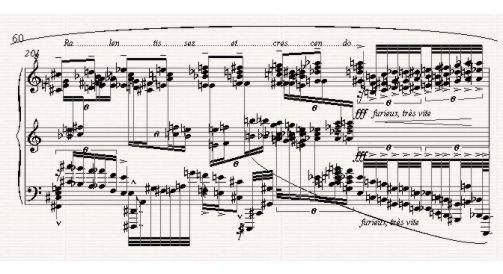
\includegraphics[width=\textwidth]{images/piano.jpg}
    \caption{Ejemplo de partitura de piano compleja, extraída de una pieza de Kaikhosru Shapurji Sorabji}
    \label{fig::partitura}
  \end{center}
\end{figure}


\cite{Melzack2001} relaciona el dolor crónico y patológico con la neuroplasticidad\index{neuroplasticidad}. Para ello estudia el {\it síndrome del miembro fantasma} ---percepción de sensaciones de que un miembro amputado todavía forma parte del cuerpo y funciona correctamente---. Antiguamente se solía pensar que estas sensaciones se debían a que el cerebro seguía recibiendo mensajes de los nervios que originalmente llevaban impulsos desde el miembro amputado. Sin embargo, la creencia actual se basa en que el cerebro sigue conservando un área dedicada a dicho miembro, por lo que el individuo sigue ``sintiéndolo''. Los estímulos sensoriales actúan sobre sistemas neuronales que fueron modificados por entradas anteriores, y su comportamiento y salida están influenciados por la ``memoria'' de esos eventos del pasado. \cite{Melzack2001} relaciona esto con la neuroplasticidad\index{neuroplasticidad} en el sentido en que en la mayoría de casos la sensación del miembro fantasma desaparece, al menos de forma temporal, sometiendo a los individuos a visiones que revelen la no correspondencia entre el miembro real y el percibido.

El estrés crónico ---el cual puede derivar en depresión--- interrumpe la neuroplasticidad de forma temporal, explica \cite{Pittenger2008}, mientras que un tratamiento antidepresivo ofrece el resultado opuesto.

Yendo más lejos, en \cite{May2008} se desarrolla la idea del {\it cambio cualitativo}\index{cambio cualitativo} ---aprendizaje de nuevas tareas--- como principal impulsor de la modificación estructural del cerebro, por encima de la práctica reiterada de un ejercicio conocido. Para ello se estudia el efecto del aprendizaje de juegos malabares por parte de 20 individuos, observando cómo este ejercicio produce una alteración de la materia gris del {\it córtex occipitotemporal}\index{córtex/corteza!occipitotemporal} con tan sólo una semana de entrenamiento.

\subsection{Memoria (Memory)}

\subsubsection{Memoria de trabajo}
\label{sec::memoria-trabajo}
En \cite{Jaeggi2008} se estudia la forma de estimular la memoria de trabajo a lo largo de cuatro experimentos, empleados para mejorar lo que denomina ``{\it inteligencia fluida}''. Ésta es una habilidad compleja humana que posibilita la adaptación del pensamiento a nuevas situaciones o problemas a los que nunca antes nos habíamos enfrentado.

El hecho de mejorar la memoria de trabajo como un medio para conseguir un fin mayor, como el mencionado, pone de manifiesto la importancia de este tipo de memoria, que es empleada en la resolución de problemas o realización de tareas complejas.

La memoria de trabajo también es empleada como medio para conseguir un objetivo diferente ---y más ambicioso si cabe--- en \cite{Olesen2004}. El texto relata como, mediante la estimulación de la memoria de trabajo a través de diversos experimentos, se consigue incrementar la actividad prefrontal y parietal del cerebro. Si recordamos la diferenciación de los lóbulos cerebrales expuesta en la sección \ref{sec:lobulos}, los lóbulos prefrontal\index{lóbulo!frontal} y parietal\index{lóbulo!parietal} albergan el procesamiento de emociones y de la información sensorial, respectivamente.

\subsubsection{Recuerdo espacial (Spatial recall)}

Este aspecto funcional del cerebro se encarga del almacenamiento a largo plazo de representaciones visuales. Una forma elegante de explicar su comportamiento es mediante la creación de un modelo del mismo, como hace \cite{becker}, y la posterior simulación de su comportamiento en entornos complejos. La lectura relata el efecto de daños cerebrales artificiales producidos sobre el modelo, concretamente en lóbulo parietal\index{lóbulo!parietal}, y utilizan sus resultados para la realización de predicciones sobre la representación neural que tiene lugar en el cerebro.

En lineas generales, el modelo consiste en lo siguiente: un {\it parahipocampo}\footnote{Estructura compleja que recubre el hipocampo por su parte inferior. También es denominado {\it circonvolución parahipocámpica}} genera una representación alocéntrica de los objetos a partir de un {\it flujo visual ventral} ---qué es el objeto---, mientras que el lóbulo parietal\index{lóbulo!parietal} interpreta un {\it flujo visual dorsal} para generar una representación egocéntrica ---dónde se encuentra el objeto---. Una conexión bidireccional recurrente entre las regiones egocéntrica y alocéntrica produce la memoria a largo plazo.

Atendiendo al objetivo del presente proyecto, resulta de aún más interés el estudio de \cite{Hirvasoja2004}, donde se analiza el efecto que los videojuegos pueden ejercer sobre las habilidades espaciales. Una de las hipótesis más interesantes del estudio es la existencia de un comportamiento diferente entre sexos ante la estimulación ejercida por los videojuegos. Mediante un experimento en el que algunos individuos son sometidos a la práctica de un juego 3D durante 5 horas seguidas se puede observar, entre otras cosas, que las mujeres presentan una mejora de las habilidades espaciales ligeramente mayor que los hombres.

\subsubsection{Recuerdo cara-nombre (Face-name recall)}

Denominamos {\it recuerdo cara-nombre} a la habilidad cerebral para mantener una correspondencia entre nombres de personas y sus caras. En \cite{Haxby2000} se propone un modelo estructural que explica el sistema neural encargado de esta habilidad, una de las más desarrolladas en los seres humanos frente a otros animales. No obstante, se concluye que la diferenciación fisiológica de los elementos participantes en este comportamiento es algo difusa, dando pie a la realización de otros posibles modelos que lo expliquen.

Por otro lado, \cite{Trinkler2009} muestra algunos resultados experimentales sobre el reconocimiento facial por parte de algunos voluntarios: los individuos son sometidos a la visualización de un conjunto de rostros ---de forma secuencial--- durante unos instantes, para mostrarles otro conjunto diferente (con ciertos rostros en común con el primero) después. Los individuos deben reconocer las caras que han aparecido en ambos conjuntos y las que aparecen en el segundo conjunto y no formaban parte del primero.

El hipocampo\index{hipocampo} es el absoluto protagonista en la asociación cara-nombre.

\subsection{Resolución de problemas (Problem solving)}
\label{sec::problem-solving}

\subsubsection{Aritmética (Arithmetic)}

Centrándonos en los efectos neuroplásticos relacionados con la aritmética, en \cite{Dehaene2004} se explica cómo la realización de cálculos por parte de los seres humanos se ve reflejada en la activación del \acf{SIP}\footnote{Hendidura irregular en la superficie convexa del lóbulo parietal, que marca la división entre los lóbulos parietales\index{lóbulo!parietal} superior e inferior.}. Un estudio adicional que corrobora este hecho descubre que ciertas patologías de esa zona cerebral producen la denominada {\it acalculia}\index{acalculia} ---imposibilidad para la realización de cálculos matemáticos, sencillos o complejos---.

Las propuestas futuras que se realizan en \cite{Dehaene2004} abarcan la comprensión de las homologías y diferencias entre la actividad cerebral de determinados simios y los seres humanos.

\subsubsection{Razonamiento lógico (Logical reasoning)}

El razonamiento lógico tiene lugar principalmente en el lóbulo frontal\index{lóbulo!frontal}, y consiste en la habilidad para combinar procesos cognitivos y la flexibilidad para reconocimiento de patrones, extracción de conclusiones y toma de decisiones. Como recurso de interés para adentrarse en el mundo de la lógica, \cite{JulianIranzo2004} ofrece un manual completo sobre las lógicas de proposiciones y predicados, enfocado al aprendizaje por parte de personas del ámbito de la Ingeniería Informática.

El razonamiento lógico permite, partiendo de uno o más juicios, derivar la validez o falsedad de otro juicio distinto. Para \cite{DeWall2008} {\it ``el sistema de procesamiento consciente y reflexivo es vital para el razonamiento lógico''}. Por tanto, se podría afirmar que el razonamiento lógico es un proceso consciente.

\subsubsection{Razonamiento cuantitativo (Quantitative reasoning)}

Los seres humanos empleamos el razonamiento cuantitativo para realizar estimaciones. Resulta de utilidad para comparar precios de productos y cuotas, valor de impuestos, etc. Especialmente en el mundo empresarial, el razonamiento cuantitativo es empleado para la toma de decisiones de negocio y selección de estrategias.

\subsection{Atención (Attention)}

\subsubsection{Concentración (Focus)}

La concentración no es más que la capacidad para prestar atención a la información pertinente, ignorando distracciones irrelevantes. Resulta de gran importancia en situaciones que impliquen realizar una tarea como la lectura en un entorno ruidoso como una cafetería. La densidad de información que llega a nuestros sentidos es inmensa, por lo que la concentración para desechar cualquier información no relevante es de alta importancia.

En \cite{Bherer2006} se exponen los resultados obtenidos tras un experimento en el que personas jóvenes y mayores son sometidas a un cierto programa de entrenamiento centrado en el control de la atención. Los resultados indican una mejora sustancial en la atención ---gracias a la {\it neuroplasticidad}\index{neuroplasticidad}---, curiosamente equivalente en ambos grupos de edad.

\subsubsection{Campo visual (Visual field)}

El campo visual consiste en el espacio que un individuo puede ver en un momento dado sin mover sus ojos. Implica a la visión periférica y resulta de gran importancia cuando se conduce un vehículo o se practican ciertos deportes. La mejora del campo visual, por tanto, supone un mecanismo muy efectivo para mejorar también nuestro rendimiento llevando a cabo esas actividades.

El campo visual disminuye con la edad, como expone \cite{Ball1988}. Sin embargo, mediante cierto tipo de videojuegos es posible realizar mejoras importantes en esta habilidad, entre otras, tal y como expresa \cite{Green2003} en anteposición a lo que comúnmente es denominado {\it ``aprendizaje perceptivo''}\footnote{Mejora de la respuesta a estímulos mediante una exposición duradera a los mismos}.

\subsection{Velocidad (Speed)}

\subsubsection{Procesamiento de información (Information processing)}

%http://blog.lumosity.com/information-processing/

Esta habilidad mental consiste en la captura e interpretación de la información sensorial que recibimos. Realizar esta tarea de forma rápida nos permite mejores tiempos de respuesta y capacidad de adaptación frente a cambios en nuestro entorno. Una de las tareas cotidianas en las que la velocidad de procesamiento de información adquiere gran importancia es la condución.

{\it ``A medida que el ser humano envejece''}, tal y como explica \cite{Wood2005}, {\it ``el rendimiento de nuestras habilidades funcionales decrece de forma significativa''}, lo que afecta de forma directa a nuestra velocidad de procesamiento de información. No obstante, es en \cite{Karlene2007} donde se muestran resultados claros ---mediante seis estudios diferentes--- del impacto que el entrenamiento cognitivo y produce sobre la velocidad de procesamiento. Curiosamente, además, concluye que {\it ``la edad y la educación tienen un impacto muy pequeño o nulo sobre la ganancia producida por el entrenamiento''}.

\subsubsection{Orientación espacial (Spatial orientation)}

La orientación espacial consiste en encontrar la dirección deseada en movimiento en un entorno físico. Se pone de manifiesto cuando nos desplazamos por una ciudad que no conocemos, así como durante la lectura e interpretación de un mapa. Se trata de una capacidad innata en gran parte, pero que puede mejorarse mediante entrenamiento.

Esta habilidad presenta diferencias entre hombres y mujeres. Sin embargo, \cite{Jing2007} afirma que dichas diferencias desaparecen parcialmente tras la práctica de ciertos ejercicios mediante videojuegos. Por otro lado, \cite{Lynn1994} documenta los efectos del entrenamiento de la orientación espacial mediante videojuegos, así como posibles formas de medir esa mejora ---de gran interés para el proyecto que nos ocupa---.

\subsection{Flexibilidad (Flexibility)}

\subsubsection{Control de impulsos (Response inhibition)}

El control de los impulsos es una habilidad mental humana que nos diferencia del resto de animales. Nos permite priorizar acciones teniendo en mente los objetivos a los que nos enfrentamos, controlando nuestros impulsos animales. En \cite{Zheng2008} se habla del control de impulsos como la {\it ``la función cerebral más evolucionada del ser humano''}.

{\it ``Conocer cómo está implementado este control de impulsos en el cerebro es uno de los mayores problemas de la neurociencia contemporánea''}, afirma \cite{James2009}.

\subsubsection{Planificación (Planning)}

La planificación es la capacidad cerebral que posee el ser humano para priorizar diferentes tareas a lo largo de un periodo de tiempo. Resulta de gran importancia, en combinación con la capacidad para intercambiar el foco de atención entre esas tareas (habilidad que se estudiará a continuación).

\subsubsection{Conmutación de tareas (Task switching)}

La conmutación de tareas supone la adaptación al cambio en el entorno, detectando cuándo y en qué situaciones resulta más beneficioso pasar a realizar otra tarea en lugar de continuar con la que estaba en curso, así como en qué momento volver a la primera tarea. Resulta inmediata la relación de esta habilidad con lo que en computación se conoce como {\it multitarea}\footnote{Característica de los sistemas operativos modernos de permitir que varios procesos sean ejecutados (en apariencia) al mismo tiempo, compartiendo uno o más procesadores.}. Gracias a la conmutación de tareas el ser humano es capaz de cambiar su foco de atención en base a cambios ajenos a él en su contexto.

En relación con la memoria de trabajo (vista en la sección \ref{sec::memoria-trabajo}), en \cite{Klaus2004} se realiza una prueba de significación de la hipótesis de que, con una práctica adecuada, el ser humano es capaz de emplear la memoria de trabajo para ejecutar dos operaciones simultáneas.

\subsubsection{Fluidez verbal (Verbal fluency)}

La fluidez verbal supone el acceso veloz al vocabulario conocido durante una conversación o tarea de escritura. Consiste en el ingenio y la capacidad de intercambio y conexión de palabras, y resulta crucial para la comunicación.

Esa conocida sensación de {\it ``tener una palabra en la punta de la lengua''} está relacionada estrechamente con la fluidez verbal. Depende de multitud de factores, como la edad, cuyo efecto se analiza en \cite{Deborah2004}.

\chapter{Método de trabajo}
\label{chap:metodo}

\drop{A}{} lo largo de este capítulo se presenta la metodología de desarrollo empleada durante el ciclo de vida del proyecto, analizando las diferentes etapas e iteraciones por las que ha pasado el mismo. Además se detallan los diferentes entregables producidos durante el proceso de desarrollo.

En primer lugar se presenta una visión global sobre el proceso de desarrollo, así como algunos detalles sobre las etapas e iteraciones por las que ha pasado el desarrollo del proyecto. En segundo lugar se estudia el análisis de requisitos del sistema, haciendo énfasis en aspectos como la calidad y la evolución, y no sólo en la funcionalidad. Después se ofrece un estudio detallado sobre los casos de uso del sistema, para dar paso al diseño e implementación del mismo. En la sección \ref{sec::implementacion} se hará también un repaso por las tecnologías empleadas para implementar BreakBrain. Por último se presentará la documentación de pruebas.

\section{Proceso Unificado de Desarrollo}
\label{sec::pud}

Para este proyecto se ha seguido una metodología de desarrollo iterativa, basada en el \ac{PUD} ---también conocido como \ac{RUP}---. Se trata de un \emph{``Proceso de Ingeniería del Software''}, según \cite{Rational1998}. Su meta es asegurar la producción de software de alta calidad, satisfaciendo las necesidades del usuario final y acotando la planificación y el presupuesto de una forma predecible.

\begin{figure}[h]
  \begin{center}
    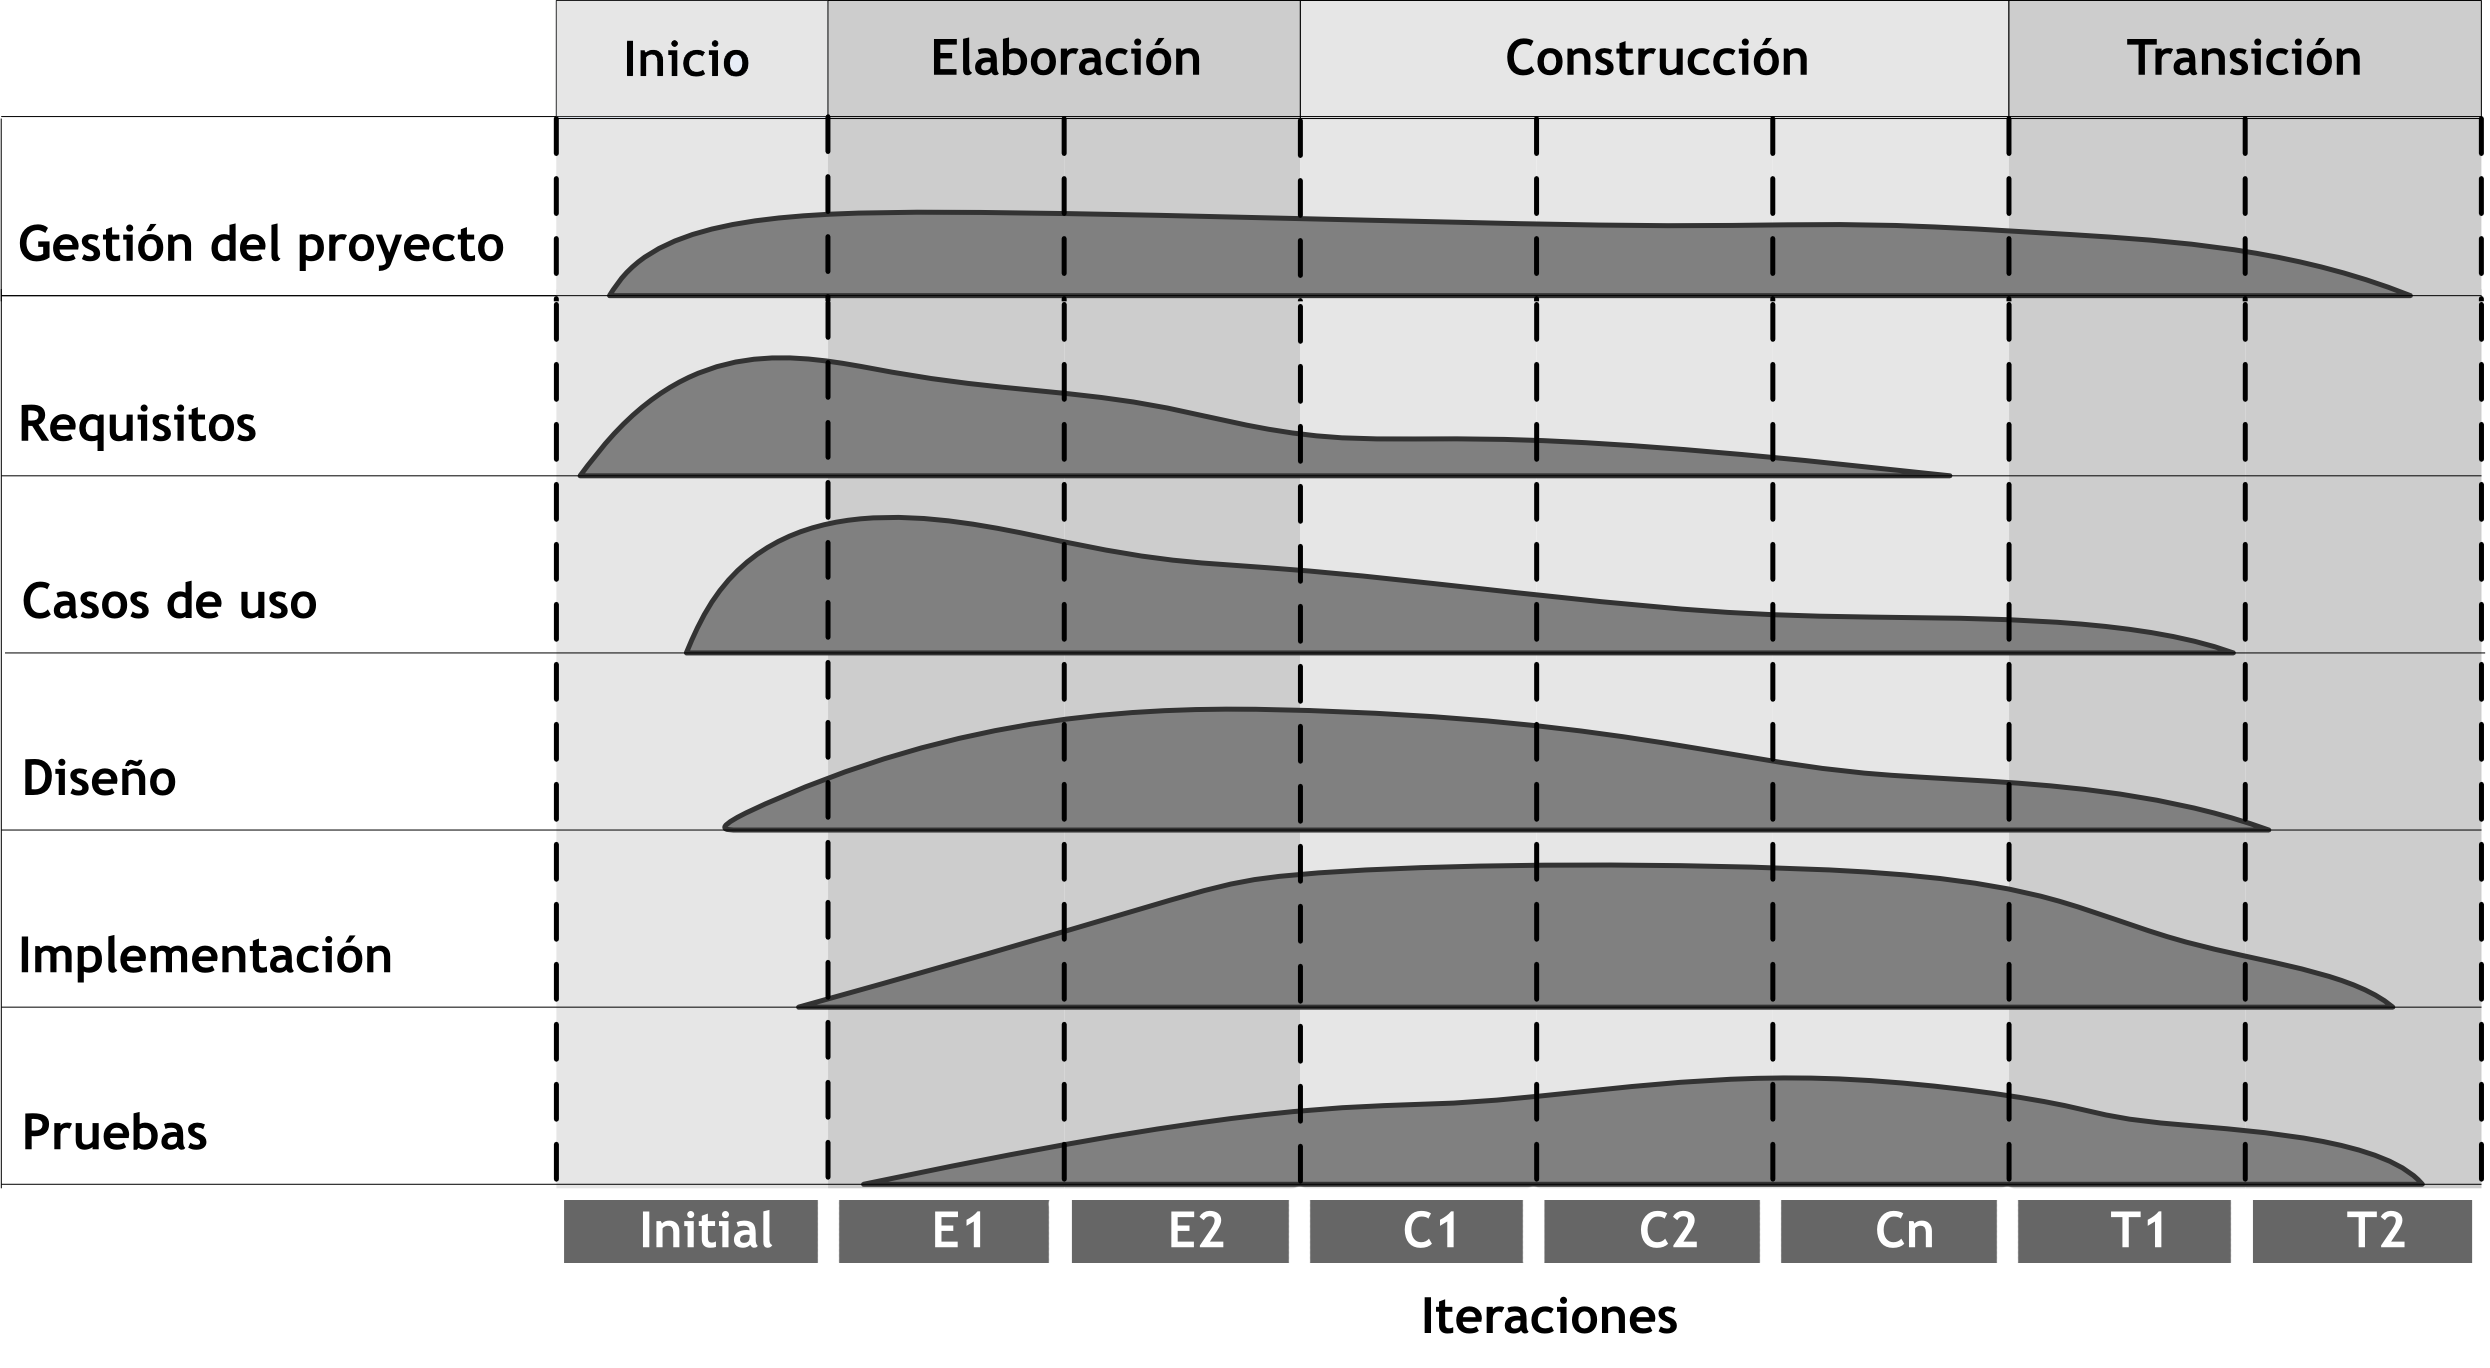
\includegraphics[width=\textwidth]{images/pud.png}
    \caption{Proceso Unificado de Desarrollo: etapas, entregables e iteraciones}
    \label{fig::pud}
  \end{center}
\end{figure}


\subsection{Visión global del proceso}

\acs{PUD} hace una clara distinción entre las dos dimensiones sobre las que se fundamenta el proceso, una dimensión estática y una dimensión dinámica:

\begin{itemize}
\item El eje horizontal representa el tiempo, y hace referencia al aspecto dinámico del proceso, en términos de \emph{etapas} e \emph{iteraciones}.
\item El eje vertical representa el aspecto estático del proceso, descrito en forma de \emph{actividades}, \emph{flujos de trabajo} o \emph{artefactos}\index{artefacto}.
\end{itemize}

En la figura \ref{fig::pud} se presenta gráficamente la estructuración del \acl{PUD} a lo largo de las dos dimensiones mencionadas.

\subsection{Etapas e iteraciones (dimensión dinámica)}

Tal y como se detalla en \cite{Rational1998}, el ciclo de vida del software según el \acl{PUD} se divide en 4 etapas o fases:

\begin{enumerate}
\item Fase de inicio
\item Fase de elaboración
\item Fase de construcción
\item Fase de transición
\end{enumerate}

La primera etapa, como inicio del desarrollo, tiene como finalidad el establecimiento de los requisitos del proyecto, los aspectos clave del mismo y las limitaciones conocidas para su desarrollo. En esta etapa se realiza la primera aproximación del modelo de casos de uso, y se presenta un plan de gestión del proyecto, detallando sus fases e iteraciones. Esta etapa puede concluir con la generación de un sencillo prototipo.

La fase de elaboración es la dedicada al análisis del dominio del problema, la aproximación de la arquitectura del sistema y la eliminación de los riesgos más críticos. Esta etapa es la más crítica, puesto que al finalizarla se puede considerar por terminada la \emph{ingeniería dura}. El diseño del sistema es el protagonista de esta fase. El análisis de requisitos y el modelo de casos de uso se dejan prácticamente terminados, y se da comienzo a la implementación.

La etapa de construcción es dedicada a desarrollar todos los componentes restantes y a integrarlos en el producto. Todas las características del software son probadas. Los esfuerzos se centran en la gestión de recursos y el control de operaciones para optimizar los costes, planificación y calidad. En esta etapa se crean los manuales de usuario.

El propósito de la fase de transición es la liberación del producto a la comunidad de usuarios. Una vez que el producto se entrega al usuario final, es posible que surjan problemas que corregir o se generen nuevos requisitos que deban ser implementados.

\subsection{Artefactos (dimensión estática)}

Un \emph{artefacto}\index{artefacto} es una pieza de información que es producida, modificada o utilizada por un proceso. Los artefactos son los productos tangibles del proyecto, los elementos generados durante el desarrollo hacia el producto final. Son la salida de una actividad y entrada de otra, y pueden ser modelos, documentos, archivos de código fuente, archivos ejecutables, etc.

Los artefactos generados durante el desarrollo de este proyecto, los cuales serán presentados más adelante, son los siguientes:

\begin{itemize}
\item Especificación de requisitos
\item Despliegue del sistema
\item Modelo de casos de uso
\item Diseño de la arquitectura software
\item Implementación
\item Documentación de pruebas
\end{itemize}



\section{Iteraciones}

En el apéndice \ref{chap::iteraciones} se ofrece un análisis detallado de la evolución iteracional del proceso de desarrollo del proyecto. En total se han realizado 7 iteraciones, cubriendo las etapas de Inicio, Elaboración y Construcción.

En el cuadro \ref{tabla::iteraciones} se ofrece un resumen de dichas estadísticas, mostrándose la evolución de cada artefacto con la conclusión de cada nueva iteración.


\begin{table}[h]  
  \begin{center}
    \begin{tabular}{|c|l||c||c|c||c|c|c|c|}
      \hline
      \tabheadformat
      -& -& Inicio & \multicolumn{2}{c||}{Elaboración} & \multicolumn{4}{c|}{Construcción}\\
      \hline
      \tabheadformat
      -& - & I1 & E1 & E2 & C1 & C2 & C3 & C4 \\
      \hline
      -& Duración & 75h & 50h & 50h & 75h & 125h & 80h & 70h \\
      \hline      \hline      
      \multirow{5}{*}{\begin{sideways}Artefactos\end{sideways}} & Requisitos & 53.6\% & 71.4\% & 85.7\% & 89.3\% & 96.4\% & 100\% & 100\% \\
      \cline{2-9}
      & Casos de uso & 27.8\% & 50\% & 77.8\% & 94.4\% & 100\% & 100\% & 100\%\\
      \cline{2-9}
      & Diseño & 10\% & 25\% & 75\% & 80\% & 85\% & 90\% & 95\% \\
      \cline{2-9}
      & Implementación & 0\% & 5.2\% & 17.3\% & 20.2\% & 50.8\% & 63.1\% & 75\% \\
      \cline{2-9}
      & Pruebas & 0\% & 0\% & 5\% & 10\% & 33.4\% & 59.1\% & 71\% \\
      \hline
    \end{tabular}
  \end{center}
  \caption{Evolución del proceso de desarrollo. Los porcentajes se han estimado teniendo en cuenta las líneas de código (para el caso de la implementación), la cobertura para las pruebas, y el número de elementos especificados (para el caso de los requisitos y los casos de uso)}
  \label{tabla::iteraciones}
\end{table}






\section{Análisis de requisitos}
\label{sec::requisitos}

Llegado este punto, procede estudiar los requisitos que debe satisfacer el sistema completo. En primer lugar se aproximará un listado de requisitos definidos de forma sencilla y superficial, para después realizar un análisis detallado de los mismos, siguiendo las directrices del estándar IEEE 830.

\subsection{Primera aproximación a los requisitos}

Para facilitar la visualización y posterior análisis de los mismos, se realiza la siguiente división:

\begin{itemize}
\item {\bf Requisitos de servidor}

  Requerimientos específicos del funcionamiento interno del sistema servidor, tanto del servidor web como del almacenamiento en base de datos y de comunicación.

\item {\bf Requisitos de usuario}

  Requerimientos asociados a la utilización por parte de un usuario. Están limitados a los aspectos referidos a los clientes del sistema.

\item {\bf Requisitos no funcionales}

  Requerimientos referidos a la seguridad, la evolución del software, al soporte, etc.


\end{itemize}

A continuación se enumeran los requisitos de cada grupo. Se trata de un análisis superficial. Con posterioridad se procederá a detallar esos requisitos.

\subsubsection{Funcionalidad referida al servidor}

La primera aproximación a los requisitos asociados al funcionamiento del sistema interno es la siguiente:

\begin{itemize}
\item El sistema debe permitir la comunicación con usuarios.
\item El sistema debe permitir almacenar y recuperar la información personal de los usuarios.
\item El sistema debe permitir almacenar y recuperar la evolución cerebral de los usuarios.
\item El sistema debe permitir recuperar listados de usuarios.
\item El sistema debe poder recomendar usuarios afines a uno dado.
\item El sistema debe poder recomendar juegos a los usuarios en base a su estado actual y evolución temporal.
\item El sistema debe ofrecer un listado con los juegos disponibles.
\item El sistema debe soportar la comunicación entre usuarios mediante mensajes escritos.
\end{itemize}


\subsubsection{Funcionalidad referida al usuario}


La primera aproximación a los requisitos asociados al usuario es la siguiente:

\begin{itemize}
\item Los usuarios podrán hacer uso de toda la web con cualquier navegador moderno, sin necesidad de plugins o componentes adicionales.
\item Los usuarios deben poder autenticarse en el sistema.
\item Los usuarios podrán cerrar su sesión.
\item Los usuarios no autenticados no deben tener acceso al resto del sitio web.
\item Los usuarios podrán registrarse.
\item El email de registro debe ser auténtico.
\item Los usuarios podrán recuperar su contraseña si no la recuerdan.
\item Los usuarios podrán seleccionar los parámetros cerebrales que deseen ejercitar.
\item Los usuarios podrán editar su información personal.
\item Los usuarios podrán seleccionar una imagen de avatar que les represente.
\item Los usuarios podrán seguir a otros usuarios.
\item Los usuarios podrán dejar de seguir a otros usuarios.
\item Los usuarios deben tener a su disposición un resumen de su evolución.
\item Los usuarios deben tener a su disposición un listado con noticias sobre los usuarios a los que sigue.
\item Los usuarios deben poder ver su perfil cerebral completo, con el estado actual y la evolución semanal, mensual y anual.
\item Los usuarios podrán hacer búsquedas de usuarios.
\item Los usuarios recibirán recomendaciones de juegos y de usuarios a los que seguir.
\item Los usuarios podrán visualizar un listado completo de juegos disponibles, diferenciando los juegos multijugador de los juegos de un solo jugador.
\item Los usuarios podrán ejecutar los juegos.
\end{itemize}

\subsubsection{Aspectos ajenos a la funcionalidad}

\begin{itemize}
\item El acceso a la base de datos debe ser rápido, para evitar esperas por parte del cliente.
\item La lógica de los juegos multijugador debe ser rápida, por lo que el servidor de juegos multijugador deberá tener muy buen rendimiento.
\item El rendimiento de los juegos deberá ser óptimo, por lo que el navegador de los clientes deberán ejecutar los juegos de forma eficiente.
\item El sistema debe soportar cientos de miles de peticiones simultáneas y responder de forma rápida y robusta.
\item El acceso al sistema debe ser controlado mediante email y contraseña.
\item Las personas no autenticadas no tendrán acceso a ninguna información ni juego.
\end{itemize}


\subsection{Requisitos funcionales}

Partiendo del análisis preliminar de requerimientos, los requisitos funcionales de los que parte el desarrollo del proyecto, basándose en el estándar IEEE 830, son los detallados a continuación. 

Para cada requisito se especifica una descripción sencilla del mismo, una valoración de su importancia (esencial, condicional u opcional), y una descripción de su validez, que incluye los mecanismos para medir su nivel de consecución, los medios para cumplir dicho requisito y una descripción de la relevancia que tiene dicho requisito en el desarrollo completo del sistema.

\renewcommand{\labelenumi}{\bf RF-\arabic{enumi}}

\begin{enumerate}

\item %%%%%%%%%%%%%%%%%%%%%%%%%%%%%%%%%%%%%%%%%%%%%%%%%%
  \begin{itemize}
  \item \underline{Descripción}: El sistema permitirá que los clientes se conecten al servidor e interactúen con la web.
  \item \underline{Importancia}: Esencial.
  \item \underline{Validez}:
    \begin{itemize}
    \item \textit{Medible}: El navegador web podrá conectarse al servidor web.
    \item \textit{Alcanzable}: El servidor ofrecerá una interfaz de peticiones GET y POST común.
    \item \textit{Relevante}: Este requisito es vital para la utilización del sistema por parte de los usuarios.
    \end{itemize}
  \end{itemize}

\item %%%%%%%%%%%%%%%%%%%%%%%%%%%%%%%%%%%%%%%%%%%%%%%%%%
  \begin{itemize}
  \item \underline{Descripción}: El sistema permitirá que los clientes intercambien mensajes con el servidor.
  \item \underline{Importancia}: Esencial.
  \item \underline{Validez}:
    \begin{itemize}
    \item \textit{Medible}: El navegador web y el servidor deben intercambiar mensajes.
    \item \textit{Alcanzable}: El servidor ofrecerá una interfaz de websockets para el intercambio de mensajes.
    \item \textit{Relevante}: Este requisito es vital para la utilización del sistema por parte de los usuarios.
    \end{itemize}
  \end{itemize}

\item %%%%%%%%%%%%%%%%%%%%%%%%%%%%%%%%%%%%%%%%%%%%%%%%%%
  \begin{itemize}
  \item \underline{Descripción}: El sistema permitirá almacenar y recuperar información personal de los usuarios.
  \item \underline{Importancia}: Esencial.
  \item \underline{Validez}:
    \begin{itemize}
    \item \textit{Medible}: El sistema recuperará la información personal de cualquier usuario dados su identificador y, por cuestiones de seguridad, su contraseña.
    \item \textit{Alcanzable}: El servidor estará conectado a una base de datos donde se almacenen y de donde se recuperen todos los datos.
    \item \textit{Relevante}: Este requisito es vital para que los usuarios puedan interactuar con el sistema.
    \end{itemize}
  \end{itemize}

\item %%%%%%%%%%%%%%%%%%%%%%%%%%%%%%%%%%%%%%%%%%%%%%%%%%
  \begin{itemize}
  \item \underline{Descripción}: El sistema permitirá almacenar y recuperar la evolución del entrenamiento cerebral de los usuarios.
  \item \underline{Importancia}: Esencial.
  \item \underline{Validez}:
    \begin{itemize}
    \item \textit{Medible}: El sistema recuperará el perfil cerebral de cualquier usuario dados su identificador y, por cuestiones de seguridad, su contraseña.
    \item \textit{Alcanzable}: El servidor estará conectado a una base de datos donde se almacenen y de donde se recuperen todos los datos.
    \item \textit{Relevante}: Este requisito es vital para que los usuarios puedan tener acceso a su evolución.
    \end{itemize}
  \end{itemize}

\item %%%%%%%%%%%%%%%%%%%%%%%%%%%%%%%%%%%%%%%%%%%%%%%%%%
  \begin{itemize}
  \item \underline{Descripción}: El sistema permitirá recuperar listados de usuarios.
  \item \underline{Importancia}: Esencial.
  \item \underline{Validez}:
    \begin{itemize}
    \item \textit{Medible}: El sistema realizará búsquedas en base a consultas textuales sencillas, obteniendo un listado con los resultados de la misma.
    \item \textit{Alcanzable}: El servidor estará conectado a una base de datos donde se almacenen todos los usuarios, y lanzará sobre ella consultas específicas.
    \item \textit{Relevante}: Este requisito es vital para que los usuarios puedan buscar a otros usuarios y empezar a seguirles, retarles a algún juego, etc.
    \end{itemize}
  \end{itemize}

\item %%%%%%%%%%%%%%%%%%%%%%%%%%%%%%%%%%%%%%%%%%%%%%%%%%
  \begin{itemize}
  \item \underline{Descripción}: El sistema recomendará juegos a los usuarios, en base a su evolución y características.
  \item \underline{Importancia}: Condicional
  \item \underline{Validez}:
    \begin{itemize}
    \item \textit{Medible}: Los usuarios tendrán en la sección de juegos un apartado con los juegos a los que el sistema les recomienda jugar, en base a su evolución cerebral.
    \item \textit{Alcanzable}: Se desarrollará un algoritmo de recomendación de juegos a usuarios basado en los parámetros cerebrales elegidos por ellos en su perfil y en la evolución de dichos parámetros a lo largo del tiempo.
    \item \textit{Relevante}: Este requisito es muy recomendable para mejorar la experiencia de usuario, además de para ayudar a mejorar las capacidades mentales en las que el usuario se vea menos hábil o cuya mejora le cueste más.
    \end{itemize}
  \end{itemize}

\item %%%%%%%%%%%%%%%%%%%%%%%%%%%%%%%%%%%%%%%%%%%%%%%%%%
  \begin{itemize}
  \item \underline{Descripción}: El sistema recomendará usuarios a los que seguir y retar, en base a sus preferencias y habilidades mentales.
  \item \underline{Importancia}: Condicional
  \item \underline{Validez}:
    \begin{itemize}
    \item \textit{Medible}: En la sección de búsqueda de usuarios de la web se ofrecerá un apartado con los usuarios más recomendables para el usuario actual.
    \item \textit{Alcanzable}: Se desarrollará un algoritmo de recomendación de personas a personas basado en los parámetros cerebrales elegidos por ellos en su perfil y en la evolución de dichos parámetros a lo largo del tiempo.
    \item \textit{Relevante}: Este requisito es muy recomendable para mejorar la experiencia de usuario, además de para ayudar a mejorar el aspecto social de BreakBrain.
    \end{itemize}
  \end{itemize}

\item %%%%%%%%%%%%%%%%%%%%%%%%%%%%%%%%%%%%%%%%%%%%%%%%%%
  \begin{itemize}
  \item \underline{Descripción}: El sistema ofrecerá un listado de juegos disponibles, permitiendo jugar a cualquiera de ellos.
  \item \underline{Importancia}: Esencial
  \item \underline{Validez}:
    \begin{itemize}
    \item \textit{Medible}: Los usuarios tendrán a su disposición un apartado de la web con todos los juegos disponibles.
    \item \textit{Alcanzable}: La web se dotará con una sección de juegos en la que se listen todos y cada uno de los juegos disponibles, categorizados por las capacidades mentales que ayudan a estimular.
    \item \textit{Relevante}: Este requisito es vital para conseguir que BreakBrain sea lo que se espera.
    \end{itemize}
  \end{itemize}

\item %%%%%%%%%%%%%%%%%%%%%%%%%%%%%%%%%%%%%%%%%%%%%%%%%%
  \begin{itemize}
  \item \underline{Descripción}: El sistema permitirá la comunicación entre usuarios mediante mensajes con el servidor.
  \item \underline{Importancia}: Esencial
  \item \underline{Validez}:
    \begin{itemize}
    \item \textit{Medible}: Los navegadores cliente de dos usuarios podrán comunicarse entre sí, de tal forma que puedan ejecutar juegos multijugador o comunicarse por medio de chat.
    \item \textit{Alcanzable}: Se emplearán websockets (un módulo en el cliente y otro en el servidor), para manterner una comunicación TCP full-duplex entre ambas partes. El servidor hará de intermediario entre dos clientes, simulando una comunicación directa entre ellos.
    \item \textit{Relevante}: Este requisito es vital para poder ofrecer juegos multijugador en la red social.
    \end{itemize}
  \end{itemize}

\item %%%%%%%%%%%%%%%%%%%%%%%%%%%%%%%%%%%%%%%%%%%%%%%%%%
  \begin{itemize}
  \item \underline{Descripción}: Los usuarios podrán hacer uso de la web completa ---incluyendo los juegos--- con cualquier navegador moderno, sin necesidad de plugins o extensiones adicionales.
  \item \underline{Importancia}: Condicional
  \item \underline{Validez}:
    \begin{itemize}
    \item \textit{Medible}: La web funcionará correctamente en diversos navegadores actuales, como las últimas versiones de Firefox, Chrome, Opera, etc.
    \item \textit{Alcanzable}: Se emplearán estándares web HTML5 y CSS3 para el desarrollo completo del sitio web, incluidos los juegos y cualquier otro componente de la red social.
    \item \textit{Relevante}: Se trata de un requisito importante, para imponer el mínimo número de restricciones al usuario final.
    \end{itemize}
  \end{itemize}


\item %%%%%%%%%%%%%%%%%%%%%%%%%%%%%%%%%%%%%%%%%%%%%%%%%%
  \begin{itemize}
  \item \underline{Descripción}: Los usuarios podrán autenticarse en el sistema para tener acceso a todo el sitio web.
  \item \underline{Importancia}: Esencial
  \item \underline{Validez}:
    \begin{itemize}
    \item \textit{Medible}: Al cargar BreakBrain se mostrará una pantalla de inicio de sesión, y ésta será la única visible hasta que el visitante inicie una sesión válida.
    \item \textit{Alcanzable}: El sitio web mantendrá un objeto de sesión con la información de usuario. Al iniciar sesión se creará dicho objeto, y al cerrarla se eliminará.
    \item \textit{Relevante}: Este es un requisito indispensable para que la web quede restringida a usuarios registrados y para que estos puedan consultar su evolución, seguir a otros usuarios, etc.
    \end{itemize}
  \end{itemize}

\item %%%%%%%%%%%%%%%%%%%%%%%%%%%%%%%%%%%%%%%%%%%%%%%%%%
  \begin{itemize}
  \item \underline{Descripción}: Los usuarios autenticados podrán cerrar su sesión.
  \item \underline{Importancia}: Condicional.
  \item \underline{Validez}:
    \begin{itemize}
    \item \textit{Medible}: En la parte superior derecha de la web (con una sesión iniciada) se mostrará un botón para cerrar sesión.
    \item \textit{Alcanzable}: El sitio web mantendrá un objeto de sesión con la información de usuario. Al iniciar sesión se creará dicho objeto, y al cerrarla se eliminará.
    \item \textit{Relevante}: Este requisito es importante para que diferentes usuarios puedan utilizar el mismo navegador.
    \end{itemize}
  \end{itemize}

\item %%%%%%%%%%%%%%%%%%%%%%%%%%%%%%%%%%%%%%%%%%%%%%%%%%
  \begin{itemize}
  \item \underline{Descripción}: Cualquier persona podrá registrarse para obtener una cuenta de usuario.
  \item \underline{Importancia}: Esencial
  \item \underline{Validez}:
    \begin{itemize}
    \item \textit{Medible}: Al acceder a BreakBrain sin una sesión iniciada, junto al formulario de login, aparecerá un formulario de registro para crear una cuenta de usuario.
    \item \textit{Alcanzable}: El sistema permitirá la creación de las estructuras de datos necesarias para la creación de un nuevo usuario, a petición de cualquier visitante desde la página de inicio.
    \item \textit{Relevante}: Es un requisito básico para que los usuarios puedan obtener una cuenta y utilizar la red social.
    \end{itemize}
  \end{itemize}

\item %%%%%%%%%%%%%%%%%%%%%%%%%%%%%%%%%%%%%%%%%%%%%%%%%%
  \begin{itemize}
  \item \underline{Descripción}: El email de registro debe ser auténtico.
  \item \underline{Importancia}: Condicional
  \item \underline{Validez}:
    \begin{itemize}
    \item \textit{Medible}: La red social no debe ser accesible a una cuenta de usuario hasta que el email haya sido correctamente comprobado.
    \item \textit{Alcanzable}: Durante el proceso de registro, el sistema debe asegurar que el email proporcionado es correcto. Para ello enviará a dicha dirección un enlace de activación. El usuario hará clic sobre el enlace para activar la cuenta y poder empezar a utilizarla.
    \item \textit{Relevante}: En BreakBrain, el identificador de los usuarios es su email. Por tanto, este requisito es importante para asegurar el contacto con cualquier usuario.
    \end{itemize}
  \end{itemize}

\item %%%%%%%%%%%%%%%%%%%%%%%%%%%%%%%%%%%%%%%%%%%%%%%%%%
  \begin{itemize}
  \item \underline{Descripción}: Los usuarios que no recuerden su contraseña podrán crear una nueva.
  \item \underline{Importancia}: Condicional
  \item \underline{Validez}:
    \begin{itemize}
    \item \textit{Medible}: La pantalla de inicio mostrará la posibilidad de solicitar un cambio de contraseña. Éste enviará un email al usuario, con un enlace de uno sólo uso que permita crear una nueva contraseña.
    \item \textit{Alcanzable}: Existirá una pantalla de establecimiento de contraseña, cuyo uso está restringido al acceso mediante enlaces generados por BreakBrain para los usuarios que lo soliciten. La base de datos mantendrá un hash por usuario, que será el utilizado para identificar un cambio de contraseña, generado cada vez que se utilice el anterior, para asegurar un único uso.
    \item \textit{Relevante}: Se trata de un requisito opcional, pero indispensable en caso de olvido de la contraseña.
    \end{itemize}
  \end{itemize}

\item %%%%%%%%%%%%%%%%%%%%%%%%%%%%%%%%%%%%%%%%%%%%%%%%%%
  \begin{itemize}
  \item \underline{Descripción}: Los usuarios podrán seleccionar qué parámetros cerebrales desean ejercitar y monitorizar.
  \item \underline{Importancia}: Condicional
  \item \underline{Validez}:
    \begin{itemize}
    \item \textit{Medible}: El perfil de usuario permitirá seleccionar las capacidades mentales que el usuario desee.
    \item \textit{Alcanzable}: La persistencia mantendrá un perfil cerebral con las capacidades mentales que deben ser consideradas por los algoritmos de recomendación y demás componentes del proyecto. Sólo los parámetros cerebrales que el usuario desee trabajar deberán ser tenidos en cuenta.
    \item \textit{Relevante}: Este requisito es importante para personalizar el entrenamiento cerebral. Si no se satisface, los usuarios no podrán priorizar las capacidades mentales.
    \end{itemize}
  \end{itemize}

\item %%%%%%%%%%%%%%%%%%%%%%%%%%%%%%%%%%%%%%%%%%%%%%%%%%
  \begin{itemize}
  \item \underline{Descripción}: Los usuarios podrán editar su información personal.
  \item \underline{Importancia}: Opcional
  \item \underline{Validez}:
    \begin{itemize}
    \item \textit{Medible}: El perfil le permitirá al usuario modificar su información personal.
    \item \textit{Alcanzable}: BreakBrain permitirá modificar todos los datos personales, menos el email, puesto que es el identificador de usuario y su autenticidad fue comprobada durante el proceso de registro.
    \item \textit{Relevante}: Es un requisito interesante para mejorar la experiencia de usuario.
    \end{itemize}
  \end{itemize}

\item %%%%%%%%%%%%%%%%%%%%%%%%%%%%%%%%%%%%%%%%%%%%%%%%%%
  \begin{itemize}
  \item \underline{Descripción}: Los usuarios podrán seleccionar una imagen de avatar para que les represente en la red.
  \item \underline{Importancia}: Opcional
  \item \underline{Validez}:
    \begin{itemize}
    \item \textit{Medible}: El perfil de usuario permitirá visualizar y modificar la imagen representativa del mismo.
    \item \textit{Alcanzable}: BreakBrain permitirá modificar los datos personales, incluida la imagen de avatar.
    \item \textit{Relevante}: Este requisito es poco importante, pero ayudará al usuario a mantener una imagen deseada frente al resto de usuarios, por lo que mejorará la experiencia de uso.
    \end{itemize}
  \end{itemize}

\item %%%%%%%%%%%%%%%%%%%%%%%%%%%%%%%%%%%%%%%%%%%%%%%%%%
  \begin{itemize}
  \item \underline{Descripción}: Los usuarios podrán comenzar a seguir a otros usuarios.
  \item \underline{Importancia}: Esencial
  \item \underline{Validez}:
    \begin{itemize}
    \item \textit{Medible}: La pantalla de exploración de usuarios permitirá comenzar a seguir a cualquier usuario.
    \item \textit{Alcanzable}: La persistencia mantendrá las estructuras de datos necesarias para almacenar qué usuarios siguen a qué otros usuarios.
    \item \textit{Relevante}: Este requisito es fundamental para mantener la componente social del proyecto.
    \end{itemize}
  \end{itemize}

\item %%%%%%%%%%%%%%%%%%%%%%%%%%%%%%%%%%%%%%%%%%%%%%%%%%
  \begin{itemize}
  \item \underline{Descripción}: Los usuarios podrán dejar de seguir a los usuarios a los que siguen.
  \item \underline{Importancia}: Esencial
  \item \underline{Validez}:
    \begin{itemize}
    \item \textit{Medible}: La pantalla de exploración de usuarios permitirá dejar de seguir a cualquier usuario.
    \item \textit{Alcanzable}: La persistencia mantendrá las estructuras de datos necesarias para almacenar qué usuarios siguen a qué otros usuarios.
    \item \textit{Relevante}: Este requisito es fundamental para mantener la componente social del proyecto.
    \end{itemize}
  \end{itemize}

\item %%%%%%%%%%%%%%%%%%%%%%%%%%%%%%%%%%%%%%%%%%%%%%%%%%
  \begin{itemize}
  \item \underline{Descripción}: Los usuarios podrán consultar un resumen de su evolución en la página de inicio.
  \item \underline{Importancia}: Condicional
  \item \underline{Validez}:
    \begin{itemize}
    \item \textit{Medible}: La pantalla principal mostrará un pequeño resumen de la evolución del perfil cerebral.
    \item \textit{Alcanzable}: El sistema deberá dar acceso a sólo parte del perfil cerebral y su evolución. La página principal mostrará, entre otras cosas, esa información resumida.
    \item \textit{Relevante}: La satisfacción de este requisito mejorará la experiencia de usuario, evitando que el mismo tenga que acceder al perfil completo para ver cómo va evolucionando.
    \end{itemize}
  \end{itemize}

\item %%%%%%%%%%%%%%%%%%%%%%%%%%%%%%%%%%%%%%%%%%%%%%%%%%
  \begin{itemize}
  \item \underline{Descripción}: Los usuarios podrán consultar un listado de novedades sobre los usuarios a los que siguen en la página de inicio.
  \item \underline{Importancia}: Condicional
  \item \underline{Validez}:
    \begin{itemize}
    \item \textit{Medible}: La página principal del sitio web mostrará las novedades de los usuarios a los que se sigue.
    \item \textit{Alcanzable}: El perfil de cada usuario incluirá un pequeño listado de novedades. Los usuarios que sigan a uno dado, y sólo ellos, tendrán acceso a dicho listado.
    \item \textit{Relevante}: La satisfacción de este requisito mejorará la experiencia de usuario, sobre todo en el aspecto social.
    \end{itemize}
  \end{itemize}

\item %%%%%%%%%%%%%%%%%%%%%%%%%%%%%%%%%%%%%%%%%%%%%%%%%%
  \begin{itemize}
  \item \underline{Descripción}: Los usuarios podrán ver su perfil cerebral completo, con el estado actual y la evolución semanal, mensual y anual.
  \item \underline{Importancia}: Esencial
  \item \underline{Validez}:
    \begin{itemize}
    \item \textit{Medible}: La web contará con una página dedicada al perfil y evolución cerebral.
    \item \textit{Alcanzable}: El sistema manejará una estructura de datos compleja con toda la información relevante referida al cerebro. Esta información incluirá el estado actual y la evolución del mismo a lo largo del tiempo.
    \item \textit{Relevante}: Se trata de un requisito vital para alcanzar los objetivos del proyecto.
    \end{itemize}
  \end{itemize}

\item %%%%%%%%%%%%%%%%%%%%%%%%%%%%%%%%%%%%%%%%%%%%%%%%%%
  \begin{itemize}
  \item \underline{Descripción}: Los usuarios podrán hacer búsquedas de usuarios.
  \item \underline{Importancia}: Esencial
  \item \underline{Validez}:
    \begin{itemize}
    \item \textit{Medible}: Existirá una página de exploración de usuarios que permitirá realizar búsquedas filtradas sobre todo el directorio de usuarios.
    \item \textit{Alcanzable}: Se desarrollará un algoritmo de búsqueda de usuarios, y será puesto a disposición de todos los usuarios mediante un sencillo formulario de búsqueda.
    \item \textit{Relevante}: Este requisito es de obligado cumplimiento para mantener un aspecto social completo en el proyecto, permitiendo que los usuarios puedan encontrar a otros usuarios y comenzar a seguirlos, dejar de seguirlos, retarles a juegos multijugador, etc.
    \end{itemize}
  \end{itemize}

\item %%%%%%%%%%%%%%%%%%%%%%%%%%%%%%%%%%%%%%%%%%%%%%%%%%
  \begin{itemize}
  \item \underline{Descripción}: Los usuarios recibirán recomendaciones de juegos.
  \item \underline{Importancia}: Condicional
  \item \underline{Validez}:
    \begin{itemize}
    \item \textit{Medible}: La web mostrará un apartado con juegos recomendados para el usuario actual.
    \item \textit{Alcanzable}: Se desarrollará un algoritmo de recomendación de juegos completo, basado en la evolución cerebral de los usuarios y su afinidad a cada tipo de juegos.
    \item \textit{Relevante}: Se trata de un requerimiento importante para mejorar la experiencia de usuario y asegurar una mejora cerebral equilibrada, reforzando las capacidades en los que el usuario flaquee más.
    \end{itemize}
  \end{itemize}

\item %%%%%%%%%%%%%%%%%%%%%%%%%%%%%%%%%%%%%%%%%%%%%%%%%%
  \begin{itemize}
  \item \underline{Descripción}: Los usuarios recibirán recomendaciones de usuarios a los que seguir.
  \item \underline{Importancia}: Condicional.
  \item \underline{Validez}:
    \begin{itemize}
    \item \textit{Medible}: La web mostrará un apartado con usuarios recomendados para el usuario actual.
    \item \textit{Alcanzable}: Se desarrollará un algoritmo de recomendación de juegos completo, basado en la evolución cerebral de los usuarios y su afinidad a cada tipo de juegos.
    \item \textit{Relevante}: Es un requisito importante para mejorar la experiencia de usuario.
    \end{itemize}
  \end{itemize}

\item %%%%%%%%%%%%%%%%%%%%%%%%%%%%%%%%%%%%%%%%%%%%%%%%%%
  \begin{itemize}
  \item \underline{Descripción}: Los usuarios podrán visualizar un listado completo de juegos disponibles, diferenciando los juegos multijugador de los juegos de un sólo jugador.
  \item \underline{Importancia}: Esencial
  \item \underline{Validez}:
    \begin{itemize}
    \item \textit{Medible}: La web ofrecerá un listado con todos los juegos disponibles, permitiendo que el usuario ejecute el que desee.
    \item \textit{Alcanzable}: El sistema mantendrá un catálogo categorizado con todos los juegos disponibles.
    \item \textit{Relevante}: Este requisito es vital para satisfacer los objetivos de BreakBrain.
    \end{itemize}
  \end{itemize}

\item %%%%%%%%%%%%%%%%%%%%%%%%%%%%%%%%%%%%%%%%%%%%%%%%%%
  \begin{itemize}
  \item \underline{Descripción}: Los usuarios podrán retar a otros usuarios y ser retados para jugar a juegos multijugador.
  \item \underline{Importancia}: Condicional
  \item \underline{Validez}:
    \begin{itemize}
    \item \textit{Medible}: La web ofrecerá un listado con todos los juegos disponibles, permitiendo que el usuario ejecute el que desee. En caso de ser un juego multijugador permitirá elegir a otro usuario contra el que jugar.
    \item \textit{Alcanzable}: El sistema permitirá seleccionar un usuario rival para jugar a un juego multijugador. Se enviará un mensaje de alerta al mismo para avisarle del reto y permitirle aceptarlo o rechazarlo.
    \item \textit{Relevante}: Este requisito es importante para satisfacer el objetivo social de BreakBrain.
    \end{itemize}
  \end{itemize}


\end{enumerate}

\subsection{Requisitos de evolución}

Partiendo del análisis preliminar de requerimientos, los requisitos de evolución de los que parte el desarrollo del proyecto, basándose en el estándar IEEE 830, son los siguientes:

\renewcommand{\labelenumi}{\bf EV-\arabic{enumi}}

\begin{enumerate}

\item %%%%%%%%%%%%%%%%%%%%%%%%%%%%%%%%%%%%%%%%%%%%%%%%%%
  \begin{itemize}
  \item \underline{Descripción}: El sistema debe soportar la integración de juegos desarrollados por terceros.
  \item \underline{Importancia}: Condicional
  \item \underline{Validez}:
    \begin{itemize}
    \item \textit{Medible}: Cualquier persona podrá crear juegos para la red social.
    \item \textit{Alcanzable}: Existirá un cargador de juegos genérico, así como un pequeño framework de construcción de los mismos, para posibilitar la compatibilidad con el sistema de comunicación cliente-servidor del sistema.
    \item \textit{Relevante}: Es un requisito interesante para facilitar la expansión de la red social, permitiendo tener contenidos nuevos de forma frecuente.
    \end{itemize}
  \end{itemize}

\end{enumerate}

\subsection{Requisitos de soporte}

Partiendo del análisis preliminar de requerimientos, los requisitos de soporte de los que parte el desarrollo del proyecto, basándose en el estándar IEEE 830, son los siguientes:
\renewcommand{\labelenumi}{\bf SO-\arabic{enumi}}

\begin{enumerate}

\item %%%%%%%%%%%%%%%%%%%%%%%%%%%%%%%%%%%%%%%%%%%%%%%%%%
  \begin{itemize}
  \item \underline{Descripción}: El acceso a la web debe realizarse desde un navegador moderno.
  \item \underline{Importancia}: Esencial
  \item \underline{Validez}:
    \begin{itemize}
    \item \textit{Medible}: El rendimiento en navegadores obsoletos dejará mucho que desear, siendo estos incluso incompatibles con ciertos componentes de la última especificación del estándar HTML5, como el canvas.
    \item \textit{Alcanzable}: Se utilizarán elementos compatibles con Firefox 9+, Chrome/Chromium 15+, Safari 5+ y Opera 12+.
    \item \textit{Relevante}: Este requisito es de vital cumplimiento para que la experiencia de usuario sea satisfactoria.
    \end{itemize}
  \end{itemize}

\end{enumerate}

\subsection{Requisitos de calidad}

Partiendo del análisis preliminar de requerimientos, los requisitos de soporte de los que parte el desarrollo del proyecto, basándose en el estándar IEEE 830, son los siguientes:
\renewcommand{\labelenumi}{\bf CA-\arabic{enumi}}

\begin{enumerate}

\item %%%%%%%%%%%%%%%%%%%%%%%%%%%%%%%%%%%%%%%%%%%%%%%%%%
  \begin{itemize}
  \item \underline{Descripción}: Los usuarios no autenticados no podrán acceder al contenido del sitio web.
  \item \underline{Importancia}: Esencial
  \item \underline{Validez}:
    \begin{itemize}
    \item \textit{Medible}: Cuando un visitante no autenticado acceda a cualquier página de la web, éste será redireccionado a la página de inicio (login).
    \item \textit{Alcanzable}: La descarga de cualquier contenido de la web será posible únicamente desde una cuenta de usuario válida, por lo que ningún visitante no autenticado tendrá acceso a ninguna información.
    \item \textit{Relevante}: Este requisito es importante para mantener la privacidad dentro de la red social.
    \end{itemize}
  \end{itemize}

\item %%%%%%%%%%%%%%%%%%%%%%%%%%%%%%%%%%%%%%%%%%%%%%%%%%
  \begin{itemize}
  \item \underline{Descripción}: La base de datos almacenará la información de los usuarios de forma segura.
  \item \underline{Importancia}: Esencial
  \item \underline{Validez}:
    \begin{itemize}
    \item \textit{Medible}: Toda la información vital de los usuarios será almacenada de forma encriptada.
    \item \textit{Alcanzable}: Los datos sensibles de los usuarios se almacenarán de forma encriptada.
    \item \textit{Relevante}: Requisito importante para mantener la seguridad en el almacenamiento de la información.
    \end{itemize}
  \end{itemize}

\item %%%%%%%%%%%%%%%%%%%%%%%%%%%%%%%%%%%%%%%%%%%%%%%%%%
  \begin{itemize}
  \item \underline{Descripción}: La comunicación entre el cliente y el servidor será segura.
  \item \underline{Importancia}: Esencial
  \item \underline{Validez}:
    \begin{itemize}
    \item \textit{Medible}: Toda la información vital de los usuarios será enviada al servidor de forma encriptada.
    \item \textit{Alcanzable}: Los datos sensibles de los usuarios se encriptarán localmente antes de ser enviados al servidor.
    \item \textit{Relevante}: Requisito muy importante para garantizar la seguridad de la transmisión de información.
    \end{itemize}
  \end{itemize}


\item %%%%%%%%%%%%%%%%%%%%%%%%%%%%%%%%%%%%%%%%%%%%%%%%%%
  \begin{itemize}
  \item \underline{Descripción}: La información de sesión local se almacenará de forma segura.
  \item \underline{Importancia}: Esencial
  \item \underline{Validez}:
    \begin{itemize}
    \item \textit{Medible}: La información sensible que se permanezca guardada localmente será ilegible.
    \item \textit{Alcanzable}: Los datos sensibles serán encriptados antes de almacenarse de forma local.
    \item \textit{Relevante}: Requisito importante para mantener la seguridad del software.
    \end{itemize}
  \end{itemize}

\item %%%%%%%%%%%%%%%%%%%%%%%%%%%%%%%%%%%%%%%%%%%%%%%%%%
  \begin{itemize}
  \item \underline{Descripción}: El servidor debe ofrecer tiempos de respuesta muy bajos, para evitar retardos en el uso de la web o los juegos.
  \item \underline{Importancia}: Esencial
  \item \underline{Validez}:
    \begin{itemize}
    \item \textit{Medible}: La utilización de la web debe ser fluida.
    \item \textit{Alcanzable}: Se desarrollará un servidor con buen rendimiento y tiempos de respuesta bajos. Se utilizará MongoDB como base de datos, para asegurar un rendimiento óptimo en la recuperación de información.
    \item \textit{Relevante}: Cumplir este requisito será esencial para que la experiencia de usuario sea buena.
    \end{itemize}
  \end{itemize}

\item %%%%%%%%%%%%%%%%%%%%%%%%%%%%%%%%%%%%%%%%%%%%%%%%%%
  \begin{itemize}
  \item \underline{Descripción}: Los juegos deben ofrecer una interacción sencilla.
  \item \underline{Importancia}: Condicional
  \item \underline{Validez}:
    \begin{itemize}
    \item \textit{Medible}: Cualquier persona no debería tener dificultad para jugar a los juegos de la plataforma.
    \item \textit{Alcanzable}: Los controles de los juegos serán preferiblemente mediante el uso del ratón o de un número bajo de teclas. Serán intuitivos, como el uso de las flechas del teclado.
    \item \textit{Relevante}: Requisito altamente recomendable para asegurar una buena  jugabilidad.
    \end{itemize}
  \end{itemize}

\item %%%%%%%%%%%%%%%%%%%%%%%%%%%%%%%%%%%%%%%%%%%%%%%%%%
  \begin{itemize}
  \item \underline{Descripción}: El sistema debe ser escalable, es decir, debe permitir aumentar la capacidad de trabajo sin comprometer su funcionamiento y calidad normales. 
  \item \underline{Importancia}: Esencial
  \item \underline{Validez}:
    \begin{itemize}
    \item \textit{Medible}: Podrá conectarse un gran número de usuarios de forma simultánea y realizar varias peticiones de información, juegos, etc. sin que el sistema sufra pérdida de rendimiento.
    \item \textit{Alcanzable}: Se empleará NodeJS\index{nodejs} para la construcción del servidor, así como MongoDB para la persistencia.
    \item \textit{Relevante}: Este requisito es vital para el proyecto en construcción, dado que una red social puede sufrir un gran número de conexiones simultáneas.
    \end{itemize}
  \end{itemize}

\end{enumerate}



\section{Diagrama de despliegue}
\label{sec::despliegue}

En base a la caracterización del sistema producida por el análisis de requisitos desarrollado a lo largo de la sección \ref{sec::requisitos} se ha elaborado el diagrama de despliegue de la figura \ref{fig::despliegue}. Nótese que se trata de una arquitectura cliente-servidor típica.

\begin{figure}[h]
  \begin{center}
    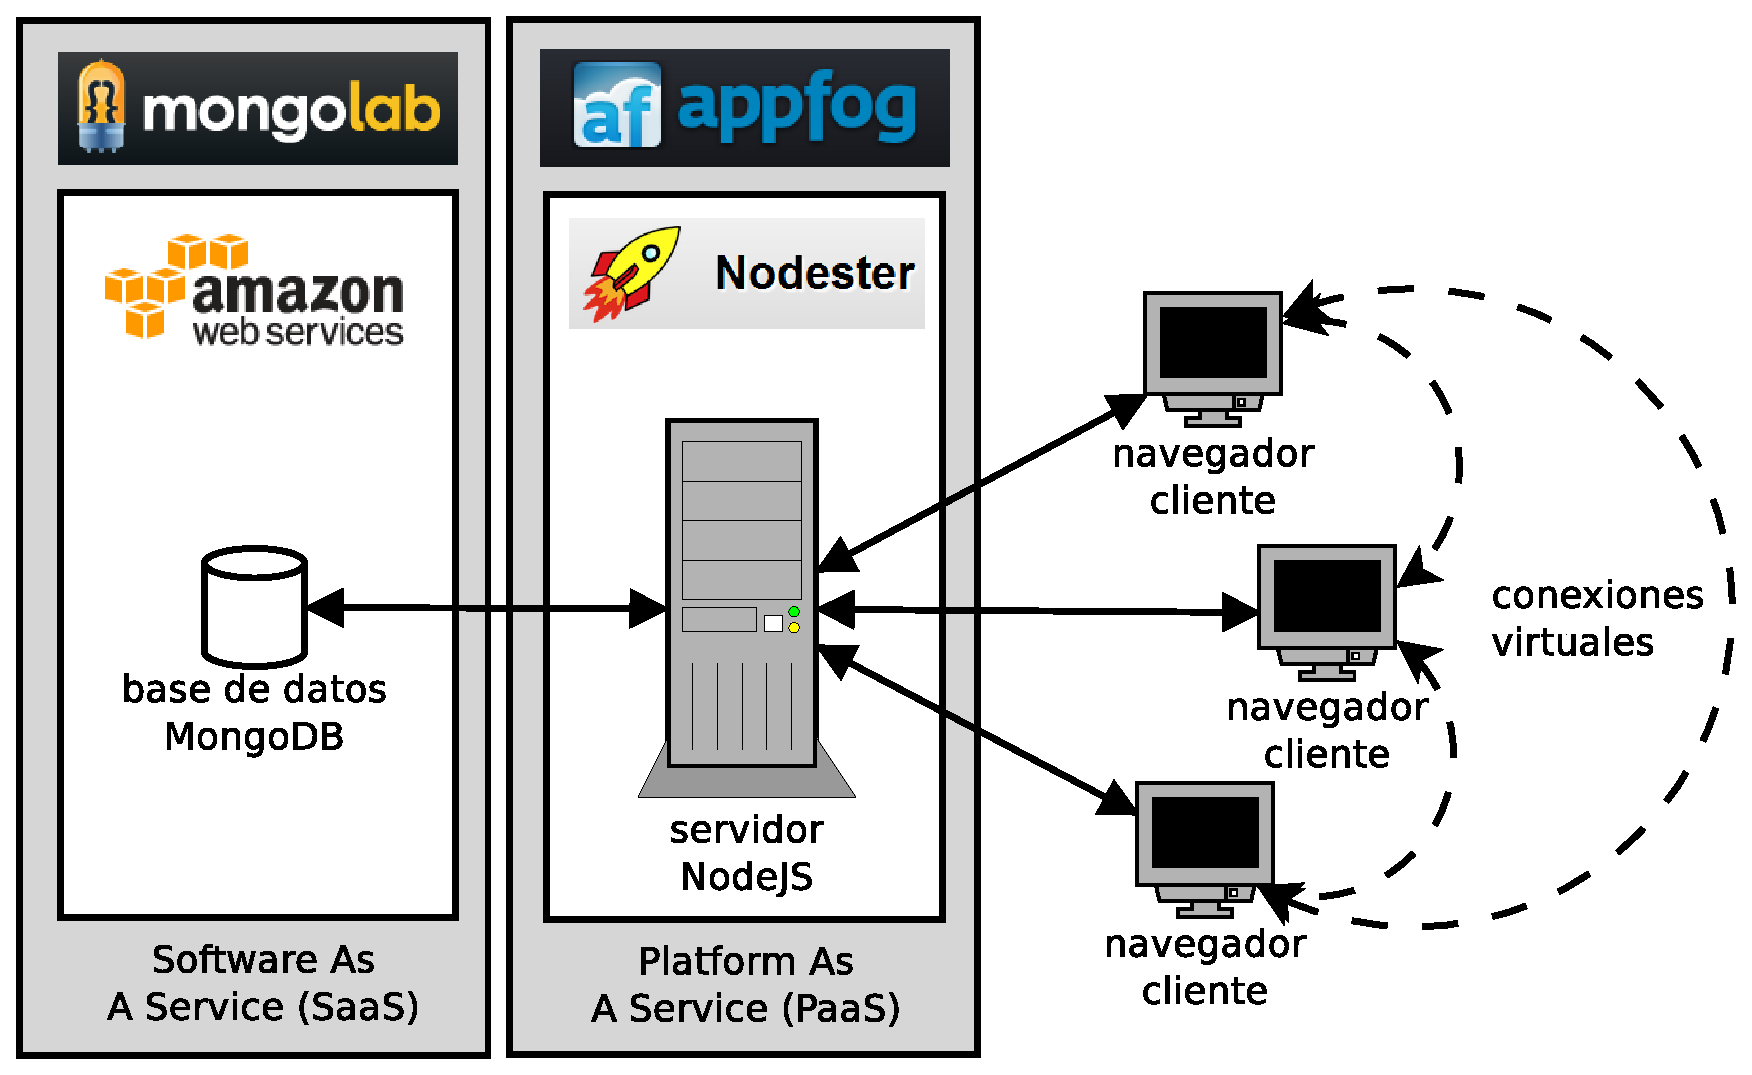
\includegraphics[width=\textwidth]{images/despliegue.eps}
    \caption{Diagrama de despliegue del sistema completo}
    \label{fig::despliegue}
  \end{center}
\end{figure}

Como puede apreciarse en la figura \ref{fig::despliegue} se emplean servicios externos que satisfacen las necesidades del sistema:

\begin{itemize}
\item Por un lado se hace uso del servicio {\bf MongoLab} \cite{Mongolab}, que proporciona un \ac{SGBD} funcionando como lo que se conoce como \ac{SAAS}, con MongoDB \cite{MongoDB}\index{mongodb} como base de datos. La persistencia de la base de datos tiene lugar en los servicios de almacenamiento web de Amazon \cite{Amazon}.
\item Por otro lado, el servidor del sistema es alojado en {\bf Nodester} \cite{Nodester}, una plataforma/hosting de aplicaciones web construidas con NodeJS \cite{NodeJS}\index{nodejs}. Este servicio pertenece a lo que se conoce como \ac{PAAS}, y es ofrecido por AppFog \cite{AppFog}.
\end{itemize}


\section{Análisis de casos de uso}
\label{sec::casos}

En esta sección se detalla el proceso seguido para la generación del artefacto correspondiente al análisis de casos de uso del sistema. En primer lugar se realiza una identificación de los actores que intervienen, para después dar paso a la identificación de los casos de uso. Por último éstos son especificados mediante una descripción, el listado de requisitos asociados, los actores que intervienen, las precondiciones y postcondiciones, los flujos de eventos y los posibles casos de uso asociados.

\subsection{Identificación  de actores}

Considerando el sistema en construcción como un único bloque, los actores que interactúan con él son los visitantes (no autenticados), los usuarios del mismo (personas autenticadas) y el sistema gestor de base de datos, al tratarse de un servicio externo. Así pues, los actores que interacturarán con los casos de uso son los siguientes:

\begin{itemize}
\item Visitante
\item Usuario
\item Sistema Gestor de Base de Datos (SGBD)
\end{itemize}

\subsection{Identificación de casos de uso}

En base al estudio de requisitos realizado en la sección \ref{sec::requisitos}, los casos de uso que se han identificado y pasarán a ser detallados como base de las etapas posteriores del desarrollo son los mostrados en la figura \ref{fig::casos}.

\begin{figure}[H]
  \begin{center}
    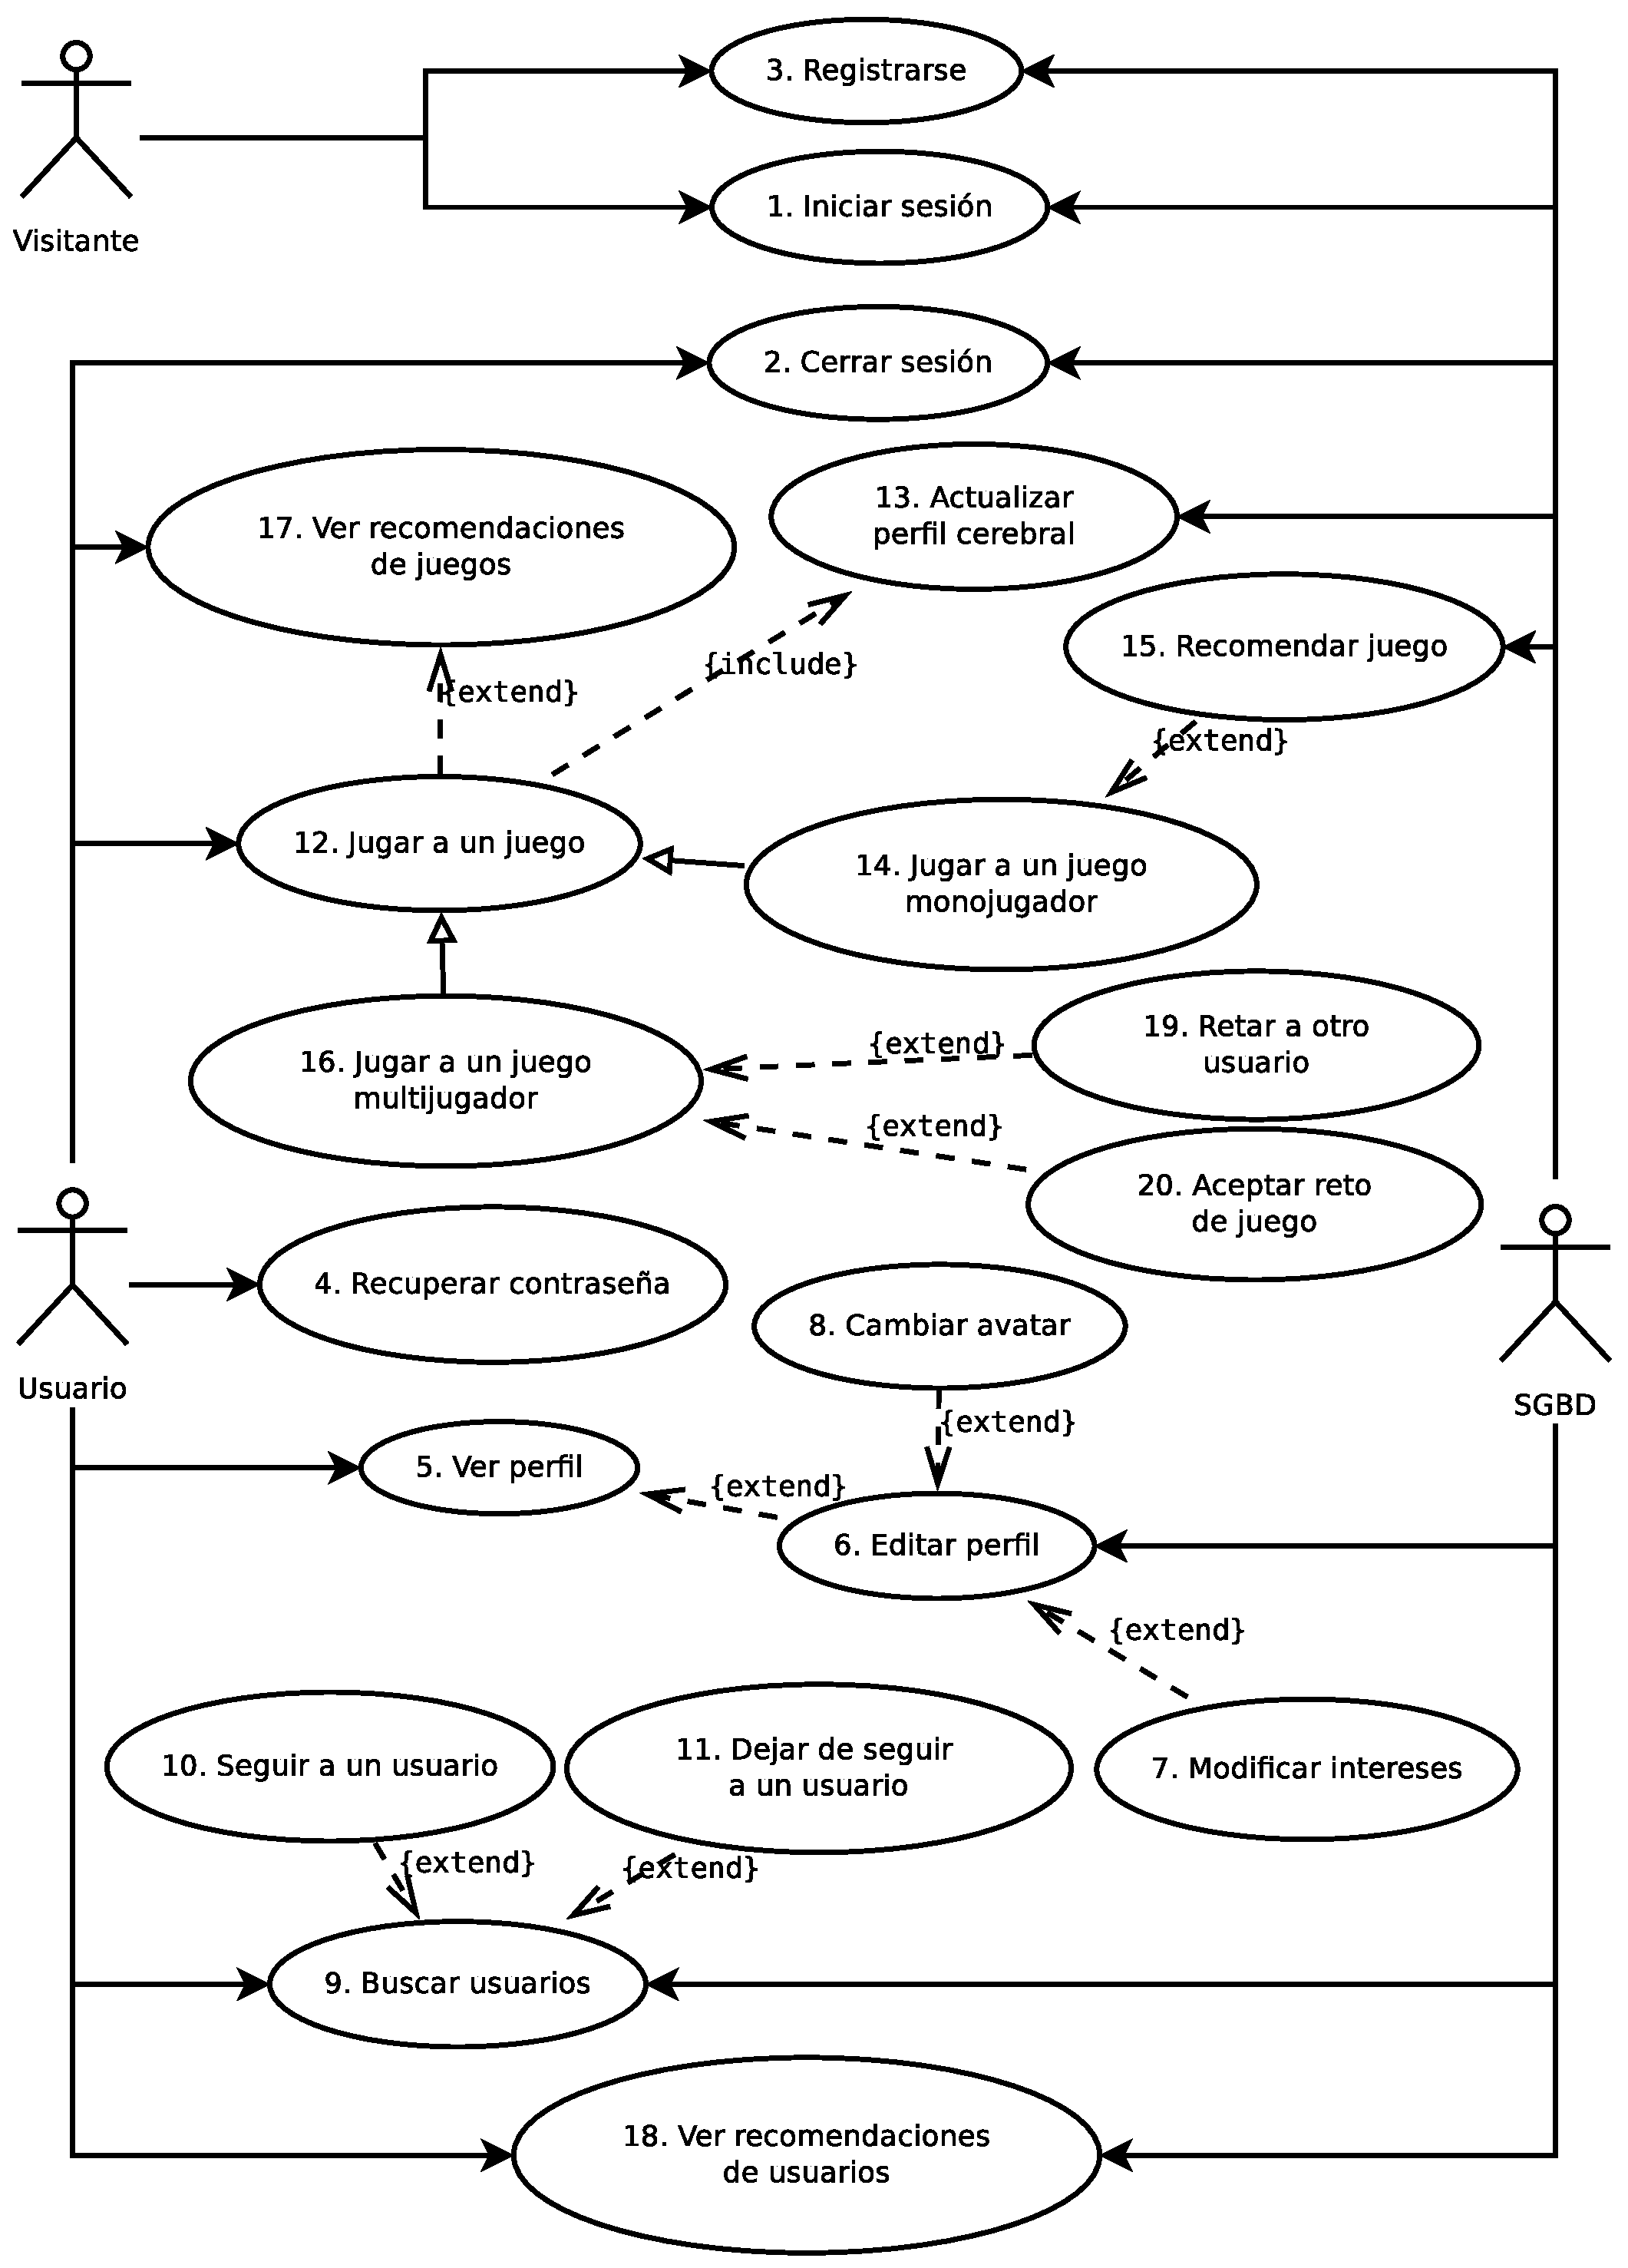
\includegraphics[width=0.9\textwidth]{images/casos-uso.eps}
    \caption{Diagrama de casos de uso}
    \label{fig::casos}
  \end{center}
\end{figure}


\subsection{Especificación de casos de uso}

A continuación se detallan todos los casos de uso identificados en la etapa anterior. Los más identificativos se acompañan, además, de un diagrama de secuencia para facilitar la comprensión del funcionamiento interno del sistema.

\renewcommand{\labelenumi}{\bf UC-\arabic{enumi}}
\renewcommand{\labelenumii}{\arabic{enumii}. }

\begin{enumerate}
\itemsep1cm
\item %%%%%%%%%%%%%%%%%%%%%%%%%%%%%%%%%%%%%%%%%%%%%%%%%%
  \begin{itemize}
  \item \textbf{Caso de uso}: Iniciar sesión
  \item \textbf{Requisito funcional asociado}: RF-11
  \item \textbf{Actores}
    \begin{itemize}
    \item Visitante
    \item SGBD
    \end{itemize}
  \item \textbf{Descripción}: Un visitante de la web inicia sesión.
  \item \textbf{Precondiciones}
    \begin{itemize}
    \item La persona no está autenticada.
    \end{itemize}
  \item \textbf{Postcondiciones}
    \begin{itemize}
    \item La persona queda autenticada (es un usuario de la red social), y tiene acceso al contenido de la web.
    \end{itemize}
  \item \textbf{Flujo normal}: autenticación exitosa (figura \ref{fig::uc-1})
    \begin{enumerate}
    \item El usuario rellena el formulario de login (email + contraseña) de la web.
    \item La web realiza la petición de envío al módulo cliente de websockets.
    \item El módulo cliente de websockets envía la petición al módulo servidor de websockets.
    \item El módulo servidor de websockets analiza la petición y se la pasa a la lógica del servidor.
    \item El módulo de lógica de servidor transforma la petición y solicita al módulo de persistencia la comprobación de los datos.
    \item El módulo de persistencia solicita al SGBD el usuario asociado al par email/contraseña.
    \item El SGBD devuelve el objeto que representa al usuario al módulo de persistencia.
    \item El módulo de persistencia transforma el objeto de usuario a la representación de dominio de un usuario y devuelve el resultado a la lógica del sistema.
    \item La lógica comprueba que el usuario es correcto y solicita su envío hacia el cliente al módulo servidor de websockets.
    \item El módulo servidor de websockets envía el objeto de usuario al módulo cliente de websockets.
    \item El módulo cliente de websockets pasa el objeto a la web.
    \item La web se actualiza con la información básica del usuario y muestra el contenido interno de la red social.
    \end{enumerate}
  \item \textbf{Flujo alternativo 1}: contraseña incorrecta o usuario inexistente
    \begin{enumerate}
    \item El usuario rellena el formulario de login (email + contraseña) de la web.
    \item La web realiza la petición de envío al módulo cliente de websockets.
    \item El módulo cliente de websockets envía la petición al módulo servidor de websockets.
    \item El módulo servidor de websockets analiza la petición y se la pasa a la lógica del servidor.
    \item El módulo de lógica de servidor transforma la petición y solicita al módulo de persistencia la comprobación de los datos.
    \item El módulo de persistencia solicita al SGBD el usuario asociado al par email/contraseña.
    \item El SGBD devuelve un error de correspondencia email/contraseña o de contraseña incorrecta.
    \item El módulo de persistencia transforma el error a la representación de dominio y lo devuelve al módulo de lógica del sistema.
    \item La lógica solicita el envío del error hacia el cliente al módulo servidor de websockets.
    \item El módulo servidor de websockets envía el error al módulo cliente de websockets.
    \item El módulo cliente de websockets pasa el error a la web.
    \item La web muestra un error de ``contraseña incorrecta'' o ``usuario inexistente'', según proceda.
    \end{enumerate}
  \item \textbf{Includes}
    \begin{itemize}
    \item Ninguno
    \end{itemize}
  \item \textbf{Extensiones}
    \begin{itemize}
    \item Ninguna
    \end{itemize}
  \item {\bf Diagrama de interacción}: Figura \ref{fig::uc-1}
  \end{itemize}


  \begin{figure}[h]
    \begin{center}
      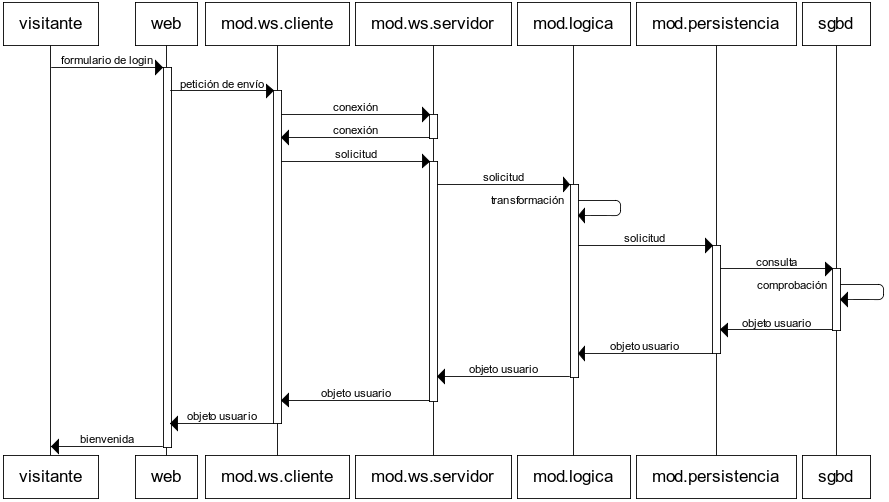
\includegraphics[width=\textwidth]{images/uc-1.png}
      \caption{Diagrama de interacción del caso de uso UC-1 (flujo normal)}
      \label{fig::uc-1}
    \end{center}
  \end{figure}


\item %%%%%%%%%%%%%%%%%%%%%%%%%%%%%%%%%%%%%%%%%%%%%%%%%%
  \begin{itemize}
  \item \textbf{Caso de uso}: Cerrar sesión
  \item \textbf{Requisito funcional asociado}: RF-12
  \item \textbf{Actores}
    \begin{itemize}
    \item Usuario
    \item SGBD
    \end{itemize}
  \item \textbf{Descripción}: Un usuario autenticado cierra su sesión.
  \item \textbf{Precondiciones}
    \begin{itemize}
    \item La persona debe tener una sesión iniciada.
    \end{itemize}
  \item \textbf{Postcondiciones}
    \begin{itemize}
    \item El acceso al contenido de la web se cierra y el usuario pasa a ser considerado como un visitante.
    \end{itemize}
  \item \textbf{Flujo normal}
    \begin{enumerate}
    \item El usuario pulsa el botón de cerrar sesión.
    \item El navegador elimina la información de sesión, y muestra la pantalla de inicio de sesión, evitando el acceso al contenido de la web.
    \end{enumerate}
  \item \textbf{Includes}
    \begin{itemize}
    \item Ninguno
    \end{itemize}
  \item \textbf{Extensiones}
    \begin{itemize}
    \item Ninguna
    \end{itemize}
  \end{itemize}

\item %%%%%%%%%%%%%%%%%%%%%%%%%%%%%%%%%%%%%%%%%%%%%%%%%%
  \begin{itemize}
  \item \textbf{Caso de uso}: Registrarse
  \item \textbf{Requisito funcional asociado}: RF-13
  \item \textbf{Actores}
    \begin{itemize}
    \item Visitante
    \item SGBD
    \end{itemize}
  \item \textbf{Descripción}: Un visitante de la web se registra para obtener una cuenta de usuario.
  \item \textbf{Precondiciones}
    \begin{itemize}
    \item La persona no está autenticada.
    \end{itemize}
  \item \textbf{Postcondiciones}
    \begin{itemize}
    \item Existe una nueva cuenta de usuario.
    \end{itemize}
  \item \textbf{Flujo normal}: registro exitoso
    \begin{enumerate}
    \item El usuario rellena el formulario de registro.
    \item La web realiza la petición de envío al módulo cliente de websockets.
    \item El módulo cliente de websockets envía la petición al módulo servidor de websockets.
    \item El módulo servidor de websockets analiza la petición y se la pasa a la lógica del servidor.
    \item El módulo de lógica de servidor transforma la petición y solicita al módulo de persistencia la comprobación de los datos.
    \item El módulo de persistencia solicita al SGBD la creación del usuario.
    \item El SGBD devuelve el objeto que representa al usuario al módulo de persistencia.
    \item El módulo de persistencia transforma el objeto de usuario a la representación de dominio de un usuario y devuelve el resultado a la lógica del sistema.
    \item La lógica envía una petición de activación al módulo de email.
    \item El módulo de email envía un correo electrónico de activación al email proporcionado por el usuario.
    \item El usuario utiliza el link de activación.
    \item La web solicita el envío de activación al módulo cliente de websockets.
    \item El módulo cliente de websockets envía la petición al módulo servidor de websockets.
    \item El módulo servidor de websockets pasa la información de activación a la lógica del servidor.
    \item El módulo de lógica pasa la información de activación al módulo de persistencia.
    \item El módulo de persistencia ejecuta la consulta de activación sobre el SGBD.
    \item El SGBD activa la cuenta y devuelve una confirmación.
    \item El módulo de persistencia devuelve la confirmación al módulo de lógica.
    \item El módulo de lógica pasa la confirmación al módulo servidor de websockets.
    \item El módulo servidor de websockets envía al módulo cliente de websockets la confirmación de activación.
    \item El módulo cliente de websockets pasa la confirmación a la web.
    \item La web muestra un mensaje de activación satisfactoria.
    \end{enumerate}
  \item \textbf{Flujo alternativo 1}: email de registro ya en uso
    \begin{enumerate}
    \item El usuario rellena el formulario de registro.
    \item La web realiza la petición de envío al módulo cliente de websockets.
    \item El módulo cliente de websockets envía la petición al módulo servidor de websockets.
    \item El módulo servidor de websockets analiza la petición y se la pasa a la lógica del servidor.
    \item El módulo de lógica de servidor transforma la petición y solicita al módulo de persistencia la comprobación de los datos.
    \item El módulo de persistencia solicita al SGBD la creación del usuario.
    \item El SGBD devuelve un error de email en uso.
    \item El módulo de persistencia devuelve el error a la lógica del sistema.
    \item El módulo de lógica pasa el error al módulo servidor de websockets.
    \item El módulo servidor de websockets envía al módulo cliente de websockets el error de email en uso.
    \item El módulo cliente de websockets pasa la el error a la web.
    \item La web muestra un mensaje de error por email en uso.
    \end{enumerate}
  \item \textbf{Includes}
    \begin{itemize}
    \item Ninguno
    \end{itemize}
  \item \textbf{Extensiones}
    \begin{itemize}
    \item Ninguna
    \end{itemize}
  \item \textbf{Diagrama de interacción}: Figura \ref{fig::uc-3}
  \end{itemize}


  \begin{figure}[h]
    \begin{center}
      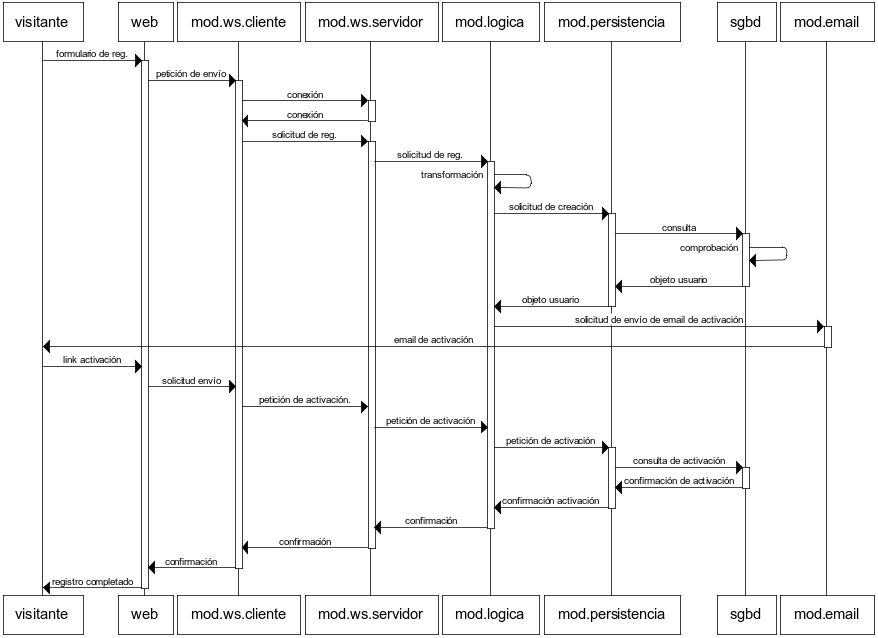
\includegraphics[width=\textwidth]{images/uc-3.png}
      \caption{Diagrama de interacción del caso de uso UC-3 (flujo normal)}
      \label{fig::uc-3}
    \end{center}
  \end{figure}

\item %%%%%%%%%%%%%%%%%%%%%%%%%%%%%%%%%%%%%%%%%%%%%%%%%%
  \begin{itemize}
  \item \textbf{Caso de uso}: Recuperar contraseña
  \item \textbf{Requisito funcional asociado}: RF-15
  \item \textbf{Actores}
    \begin{itemize}
    \item Usuario
    \item SGBD
    \end{itemize}
  \item \textbf{Descripción}: El usuario que olvidó su contraseña genera una nueva, sustituyendo ésta a la anterior.
  \item \textbf{Precondiciones}
    \begin{itemize}
    \item La persona no debe tener una sesión iniciada.
    \end{itemize}
  \item \textbf{Postcondiciones}
    \begin{itemize}
    \item La contraseña anterior del usuario queda sustituida por la nueva.
    \end{itemize}
  \item \textbf{Flujo normal}
    \begin{enumerate}
    \item El usuario hace clic sobre el enlace de recuperación de contraseña.
    \item La web le ofrece un diálogo para que introduzca el email con el que se registró.
    \item El usuario escribe su email y acepta el envío de un enlace para generar la contraseña.
    \item La web envía la solicitud al módulo de websockets cliente.
    \item El módulo cliente de websockets envía la solicitud al módulo servidor de websockets.
    \item El módulo servidor de websockets recibe la solicitud y la pasa al módulo de lógica del servidor.
    \item El módulo de lógica pasa la solicitud al módulo de persistencia.
    \item El módulo de persistencia pide el hash del objeto usuario asociado al email de la petición al SGBD.
    \item El SGBD devuelve el hash del usuario asociado al email.
    \item El módulo de persistencia devuelve el hash al módulo de lógica.
    \item El módulo de lógica genera un link y solicita al módulo de email el envío del mismo.
    \item El módulo de email envía el link a la dirección proporcionada por el usuario.
    \item El usuario sigue el enlace recibido por email y accede a la pantalla de generación de contraseña. Crea una nueva contraseña y acepta su envío.
    \item La web envía los nuevos datos al módulo cliente de websockets.
    \item El módulo cliente de websockets recibe la información y envía la solicitud de cambio de contraseña al módulo servidor de websockets.
    \item El módulo servidor de websockets pasa la petición al módulo de lógica del servidor.
    \item El módulo de lógica solicita la sobreescritura de la contraseña antigua al módulo de persistencia, y genera un hash nuevo para sobreescribir al antiguo y evitar que el link de regeneración de contraseña vuelva a usarse.
    \item El módulo de persistencia realiza las consultas pertinentes sobre el SGBD.
    \item El SGBD modifica los datos y devuelve una confirmación de que los cambios se han realizado satisfactoriamente.
    \item El módulo de persistencia devuelve la confirmación al módulo de lógica.
    \item El módulo de lógica solicita el envío de la confirmación al módulo servidor de websockets.
    \item El módulo servidor de websockets envía la confirmación al módulo cliente de websockets.
    \item El módulo cliente de websockets pasa la confirmación a la web.
    \item La web muestra un mensaje de éxito.
    \end{enumerate}
  \item \textbf{Includes}
    \begin{itemize}
    \item Ninguno
    \end{itemize}
  \item \textbf{Extensiones}
    \begin{itemize}
    \item Ninguna
    \end{itemize}
  \item \textbf{Diagrama de interacción}: Figura \ref{fig::uc-4}
  \end{itemize}
  
  \begin{figure}[h]
    \begin{center}
      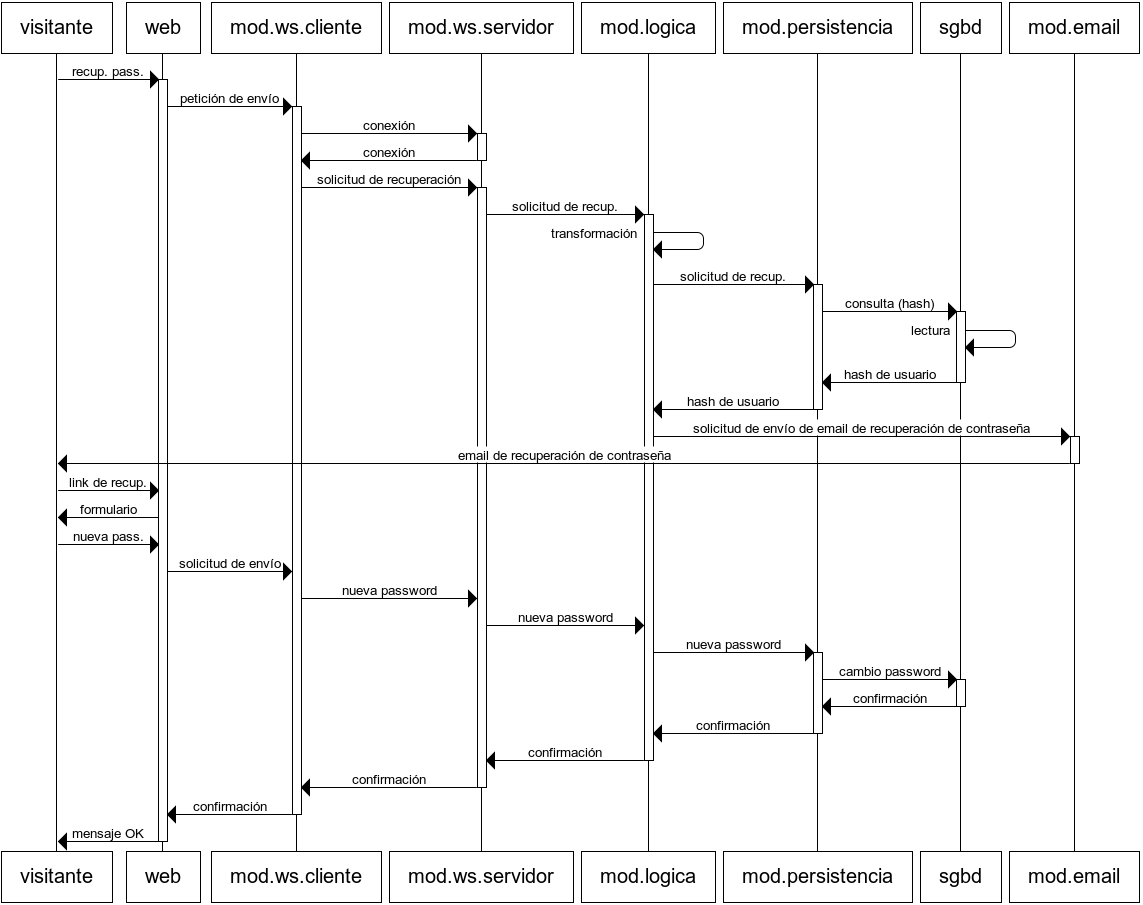
\includegraphics[width=\textwidth]{images/uc-4.png}
      \caption{Diagrama de interacción del caso de uso UC-4 (flujo normal)}
      \label{fig::uc-4}
    \end{center}
  \end{figure}

\item %%%%%%%%%%%%%%%%%%%%%%%%%%%%%%%%%%%%%%%%%%%%%%%%%%
  \begin{itemize}
  \item \textbf{Caso de uso}: Ver perfil
  \item \textbf{Requisitos funcionales asociados}: RF-16, RF-17
  \item \textbf{Actores}
    \begin{itemize}
    \item Usuario
    \item SGBD
    \end{itemize}
  \item \textbf{Descripción}: Un usuario solicita ver su perfil completo.
  \item \textbf{Precondiciones}
    \begin{itemize}
    \item El usuario está autenticado en el sistema
    \end{itemize}
  \item \textbf{Postcondiciones}
    \begin{itemize}
    \item Ninguna
    \end{itemize}
  \item \textbf{Flujo normal}
    \begin{enumerate}
    \item El usuario accede a la página de perfil.
    \item La web envía la petición de información al módulo cliente de websockets.
    \item El módulo cliente de websockets envía la petición al módulo servidor de websockets.
    \item El módulo servidor de websockets pasa la solicitud del perfil al módulo de lógica.
    \item El módulo de lógica del servidor pasa la solicitud al módulo de persistencia.
    \item El módulo de persistencia realiza una consulta sobre SGBD para recuperar el perfil de usuario.
    \item El SGBD recupera la información y se la envía de vuelta al módulo de persistencia.
    \item El módulo de persistencia devuelve el objeto de perfil al módulo de lógica.
    \item El módulo de lógica solicita el envío del perfil al módulo servidor de websockets.
    \item El módulo servidor de websockets envía la información al módulo cliente de websockets.
    \item El módulo cliente de websockets pasa toda la información de perfil a la web.
    \item La web se actualiza con la información del perfil completo.
    \end{enumerate}
  \item \textbf{Includes}
    \begin{itemize}
    \item Ninguno
    \end{itemize}
  \item \textbf{Extensiones}
    \begin{itemize}
    \item UC-6
    \end{itemize}
  \end{itemize}

\item %%%%%%%%%%%%%%%%%%%%%%%%%%%%%%%%%%%%%%%%%%%%%%%%%%
  \begin{itemize}
  \item \textbf{Caso de uso}: Editar perfil
  \item \textbf{Requisitos funcionales asociados}: RF-17
  \item \textbf{Actores}
    \begin{itemize}
    \item Usuario
    \item SGBD
    \end{itemize}
  \item \textbf{Descripción}: 
  \item \textbf{Precondiciones}
    \begin{itemize}
    \item El usuario está autenticado en el sistema.
    \end{itemize}
  \item \textbf{Postcondiciones}
    \begin{itemize}
    \item El perfil del usuario es modificado en la base de datos.
    \end{itemize}
  \item \textbf{Flujo normal}
    \begin{enumerate}
    \item El usuario accede a la página de perfil.
    \item La web envía la petición de información al módulo cliente de websockets.
    \item El módulo cliente de websockets envía la petición al módulo servidor de websockets.
    \item El módulo servidor de websockets pasa la solicitud del perfil al módulo de lógica.
    \item El módulo de lógica del servidor pasa la solicitud al módulo de persistencia.
    \item El módulo de persistencia realiza una consulta sobre SGBD para recuperar el perfil de usuario.
    \item El SGBD recupera la información y se la envía de vuelta al módulo de persistencia.
    \item El módulo de persistencia devuelve el objeto de perfil al módulo de lógica.
    \item El módulo de lógica solicita el envío del perfil al módulo servidor de websockets.
    \item El módulo servidor de websockets envía la información al módulo cliente de websockets.
    \item El módulo cliente de websockets pasa toda la información de perfil a la web.
    \item La web se actualiza con la información del perfil completo.
    \item El usuario modifica la información personal y pulsa el botón de guardar cambios.
    \item La web envía la solicitud de modificación al módulo cliente de websockets.
    \item El módulo cliente de websockets envía la solicitud al módulo servidor de websockets.
    \item El módulo servidor de websockets pasa la solicitud de modificación de perfil al módulo de lógica.
    \item El módulo de lógica pasa la solicitud al módulo de persistencia.
    \item El módulo de persistencia ejecuta las consultas de modificación sobre el SGBD.
    \item El SGBD devuelve una confirmación.
    \item El módulo de persistencia devuelve la confirmación al módulo de lógica.
    \item El módulo de lógica devuelve la confirmación al módulo servidor de websockets.
    \item El módulo servidor de websockets envía la confirmación al módulo cliente de websockets.
    \item El módulo cliente de websockets devuelve la confirmación a la web.
    \item La web se actualiza mostrando un mensaje de éxito al guardar los cambios.
    \end{enumerate}
  \item \textbf{Includes}
    \begin{itemize}
    \item Ninguno
    \end{itemize}
  \item \textbf{Extensiones}
    \begin{itemize}
    \item UC-8
    \item UC-7
    \end{itemize}
  \end{itemize}

\item %%%%%%%%%%%%%%%%%%%%%%%%%%%%%%%%%%%%%%%%%%%%%%%%%%
  \begin{itemize}
  \item \textbf{Caso de uso}: Modificar intereses
  \item \textbf{Requisitos funcionales asociados}: RF-16
  \item \textbf{Actores}
    \begin{itemize}
    \item Usuario
    \item SGBD
    \end{itemize}
  \item \textbf{Descripción}: El usuario modifica las habilidades mentales que quiere trabajar.
  \item \textbf{Precondiciones}
    \begin{itemize}
    \item El usuario debe estar autenticado en el sistema.
    \item El usuario debe estar visualizando su perfil.
    \end{itemize}
  \item \textbf{Postcondiciones}
    \begin{itemize}
    \item Los parámetros de entrenamiento cerebral (intereses mentales del usuario) se ven modificados de forma temporal (no permanente)
    \end{itemize}
  \item \textbf{Flujo normal}
    \begin{enumerate}
    \item El usuario hace clic sobre un botón para ver sus intereses actuales.
    \item La web solicita la información de intereses al módulo cliente de websockets.
    \item El módulo cliente de websockets envía la solicitud al módulo servidor de websockets.
    \item El módulo servidor de websockets recibe la petición y se la pasa al módulo de lógica del servidor.
    \item El módulo de lógica solicita la información al módulo de persistencia.
    \item El módulo de persistencia ejecuta la consulta de recuperación de intereses sobre el SGBD.
    \item El SGBD obtiene la información requerida y se la envía de vuelta al módulo de persistencia.
    \item El módulo de persistencia pasa la información de intereses al módulo de lógica.
    \item El módulo de lógica devuelve los datos al módulo servidor de websockets para que los envíe al cliente.
    \item El módulo servidor de websockets envía de vuelta la información al módulo cliente de websockets.
    \item El módulo cliente de websockets pasa la información a la web.
    \item La web muestra los intereses del usuario.
    \item El usuario modifica esos intereses.
    \end{enumerate}
  \item \textbf{Includes}
    \begin{itemize}
    \item Ninguno
    \end{itemize}
  \item \textbf{Extensiones}
    \begin{itemize}
    \item Ninguna
    \end{itemize}
  \end{itemize}

\item %%%%%%%%%%%%%%%%%%%%%%%%%%%%%%%%%%%%%%%%%%%%%%%%%%
  \begin{itemize}
  \item \textbf{Caso de uso}: Cambiar avatar
  \item \textbf{Requisitos funcionales asociados}: RF-18
  \item \textbf{Actores}
    \begin{itemize}
    \item Usuario
    \end{itemize}
  \item \textbf{Descripción}: El usuario modifica su avatar (imagen representativa).
  \item \textbf{Precondiciones}
    \begin{itemize}
    \item El usuario debe estar autenticado.
    \item El usuario debe encontrarse en la página de perfil.
    \end{itemize}
  \item \textbf{Postcondiciones}
    \begin{itemize}
    \item El avatar de usuario es cambiado de forma temporal (no permanente).
    \end{itemize}
  \item \textbf{Flujo normal}
    \begin{enumerate}
    \item El usuario hace clic sobre un botón para ``cambiar su avatar''.
    \item La web le muestra un mensaje de diálogo para que seleccione una imagen nueva desde su ordenador.
    \item El usuario selecciona una imagen y acepta.
    \item La web recupera la imagen elegida y sustituye al avatar anterior.
    \end{enumerate}
  \item \textbf{Includes}
    \begin{itemize}
    \item Ninguno
    \end{itemize}
  \item \textbf{Extensiones}
    \begin{itemize}
    \item Ninguna
    \end{itemize}
  \end{itemize}

\item %%%%%%%%%%%%%%%%%%%%%%%%%%%%%%%%%%%%%%%%%%%%%%%%%%
  \begin{itemize}
  \item \textbf{Caso de uso}: Buscar usuarios
  \item \textbf{Requisitos funcionales asociados}: RF-24
  \item \textbf{Actores}
    \begin{itemize}
    \item Usuario
    \item SGBD
    \end{itemize}
  \item \textbf{Descripción}: El usuario ejecuta una búsqueda sobre el sistema, que le devuelve un listado de usuarios coincidentes con dicha consulta.
  \item \textbf{Precondiciones}
    \begin{itemize}
    \item El usuario debe estar autenticado en la web.
    \item El usuario se encuentra visualizando la página de exploración de usuarios.
    \end{itemize}
  \item \textbf{Postcondiciones}
    \begin{itemize}
    \item Ninguna
    \end{itemize}
  \item \textbf{Flujo normal}
    \begin{enumerate}
    \item El usuario rellena el formulario de búsqueda y hace clic sobre el botón de buscar.
    \item La web construye la estructura de datos adecuada para almacenar la información del formulario y solicita su envío al módulo cliente de websockets.
    \item El módulo cliente de websockets envía la información al módulo servidor de websockets.
    \item El módulo servidor de websockets pasa la información al módulo de lógica del servidor.
    \item El módulo de lógica pasa la información de búsqueda al módulo de persistencia.
    \item El módulo de persistencia ejecuta el algoritmo de búsqueda sobre el SGBD.
    \item El SGBD devuelve un listado de resultados coincidentes con la búsqueda.
    \item El módulo de persistencia devuelve los resultados al módulo de lógica del servidor.
    \item El módulo de lógica solicita el envío de los resultados al módulo servidor de websockets.
    \item El módulo servidor de websockets envía los resultados al módulo cliente de websockets.
    \item El módulo cliente de websockets recibe los resultados y se los pasa a la web.
    \item La web se actualiza y muestra los resultados de la búsqueda.
    \end{enumerate}
  \item \textbf{Includes}
    \begin{itemize}
    \item Ninguno
    \end{itemize}
  \item \textbf{Extensiones}
    \begin{itemize}
    \item UC-10
    \item UC-11
    \end{itemize}
  \end{itemize}

\item %%%%%%%%%%%%%%%%%%%%%%%%%%%%%%%%%%%%%%%%%%%%%%%%%%
  \begin{itemize}
  \item \textbf{Caso de uso}: Seguir a un usuario
  \item \textbf{Requisitos funcionales asociados}: RF-19
  \item \textbf{Actores}
    \begin{itemize}
    \item Usuario
    \item SGBD
    \end{itemize}
  \item \textbf{Descripción}: El usuario actual se convierte en seguidor de otro usuario.
  \item \textbf{Precondiciones}
    \begin{itemize}
    \item El usuario está autenticado en la web.
    \item El usuario se encuentra en la página de exploración de usuarios.
    \item El usuario ha realizado una búsqueda de usuarios cuyo resultado incluye al usuario objetivo.
    \item El usuario actual no es seguidor del usuario al que se va a empezar a seguir.
    \end{itemize}
  \item \textbf{Postcondiciones}
    \begin{itemize}
    \item El usuario actual es seguidor del otro usuario.
    \end{itemize}
  \item \textbf{Flujo normal}
    \begin{enumerate}
    \item El usuario hace clic sobre el resultado de búsqueda asociado al usuario objetivo.
    \item La web muestra el perfil del usuario objetivo.
    \item El usuario actual hace clic sobre el botón ``seguir''.
    \item La web envía la solicitud de seguimiento al módulo cliente de websockets.
    \item El módulo cliente de websockets envía la solicitud de seguimiento al módulo servidor de websockets.
    \item El módulo de lógica pasa la solicitud al módulo de persistencia.
    \item El módulo de persistencia ejecuta la consulta de establecimiento de un nuevo seguidor sobre el SGBD.
    \item El SGBD actualiza la base de datos y devuelve una confirmación.
    \item El módulo de persistencia devuelve la confirmación al módulo de lógica del servidor.
    \item El módulo de lógica solicita el envío de la confirmación al módulo servidor de websockets.
    \item El módulo servidor de websockets envía la confirmación al módulo cliente de websockets.
    \item El módulo cliente de websockets recibe la confirmación y se los pasa a la web.
    \item La web se actualiza y muestra un mensaje de éxito.
    \end{enumerate}
  \item \textbf{Includes}
    \begin{itemize}
    \item Ninguno
    \end{itemize}
  \item \textbf{Extensiones}
    \begin{itemize}
    \item Ninguna
    \end{itemize}
  \end{itemize}


\item %%%%%%%%%%%%%%%%%%%%%%%%%%%%%%%%%%%%%%%%%%%%%%%%%%
  \begin{itemize}
  \item \textbf{Caso de uso}: Dejar de seguir a un usuario
  \item \textbf{Requisitos funcionales asociados}: RF-20
  \item \textbf{Actores}
    \begin{itemize}
    \item Usuario
    \item SGBD
    \end{itemize}
  \item \textbf{Descripción}: El usuario actual deja de ser seguidor de otro usuario.
  \item \textbf{Precondiciones}
    \begin{itemize}
    \item El usuario está autenticado en la web.
    \item El usuario se encuentra en la página de exploración de usuarios.
    \item El usuario ha realizado una búsqueda de usuarios cuyo resultado incluye al usuario objetivo.
    \item El usuario actual es seguidor del usuario al que se va a dejar de seguir.
    \end{itemize}
  \item \textbf{Postcondiciones}
    \begin{itemize}
    \item El usuario actual no es seguidor del otro usuario.
    \end{itemize}
  \item \textbf{Flujo normal}
    \begin{enumerate}
    \item El usuario hace clic sobre el resultado de búsqueda asociado al usuario objetivo.
    \item La web muestra el perfil del usuario objetivo.
    \item El usuario actual hace clic sobre el botón ``dejar de seguir''.
    \item La web envía la solicitud de anulación de seguimiento al módulo cliente de websockets.
    \item El módulo cliente de websockets envía la solicitud de anulación de seguimiento al módulo servidor de websockets.
    \item El módulo de lógica pasa la solicitud al módulo de persistencia.
    \item El módulo de persistencia ejecuta la consulta de eliminación de un seguidor sobre el SGBD.
    \item El SGBD actualiza la base de datos y devuelve una confirmación.
    \item El módulo de persistencia devuelve la confirmación al módulo de lógica del servidor.
    \item El módulo de lógica solicita el envío de la confirmación al módulo servidor de websockets.
    \item El módulo servidor de websockets envía la confirmación al módulo cliente de websockets.
    \item El módulo cliente de websockets recibe la confirmación y se los pasa a la web.
    \item La web se actualiza y muestra un mensaje de éxito.
    \end{enumerate}
  \item \textbf{Includes}
    \begin{itemize}
    \item Ninguno
    \end{itemize}
  \item \textbf{Extensiones}
    \begin{itemize}
    \item Ninguna
    \end{itemize}
  \end{itemize}

\item %%%%%%%%%%%%%%%%%%%%%%%%%%%%%%%%%%%%%%%%%%%%%%%%%%
  \begin{itemize}
  \item \textbf{Caso de uso}: Jugar a un juego
  \item \textbf{Requisitos funcionales asociados}: RF-8, RF-27
  \item \textbf{Actores}
    \begin{itemize}
    \item Usuario
    \item SGBD
    \end{itemize}
  \item \textbf{Descripción}: El usuario lanza un juego para jugar a él.
  \item \textbf{Precondiciones}
    \begin{itemize}
    \item El usuario debe estar autenticado en el sistema.
    \end{itemize}
  \item \textbf{Postcondiciones}
    \begin{itemize}
    \item El perfil cerebral es actualizado con los resultados de la partida.
    \end{itemize}
  \item \textbf{Flujo normal}
    \begin{enumerate}
    \item El usuario accede a la página de juegos.
    \item La web solicita la petición de los listados de juegos al módulo cliente de websockets.
    \item El módulo cliente de websockets envía la solicitud al módulo servidor de websockets.
    \item El módulo servidor de websockets pasa la solicitud al módulo de lógica.
    \item El módulo de lógica realiza la petición al módulo de juegos.
    \item El módulo de juegos devuelve un listado con todos los juegos disponibles.
    \item El módulo de lógica solicita el envío del listado al módulo servidor de websockets.
    \item El módulo servidor de websockets envía el listado de juegos al módulo cliente de websockets.
    \item El módulo cliente de websockets devuelve el listado de juegos a la web.
    \item La web carga la página solicitada con los juegos disponibles.
    \item El usuario selecciona un juego al que jugar.
    \item La web solicita el juego al módulo cliente de websockets.
    \item El módulo cliente de websockets envía la petición al módulo servidor de websockets.
    \item El módulo servidor de websockets pasa la petición al módulo de lógica.
    \item El módulo de lógica solicita el juego pedido al módulo de juegos.
    \item El módulo de juegos devuelve el juego solicitado completo.
    \item El módulo de lógica solicita el envío del juego al módulo servidor de websockets.
    \item El módulo servidor de websockets envía el juego al módulo cliente de websockets.
    \item El módulo cliente de websockets pasa el juego a la web.
    \item La web carga el juego recibido y lo ejecuta.
    \end{enumerate}
  \item \textbf{Includes}
    \begin{itemize}
    \item UC-13
    \end{itemize}
  \item \textbf{Extensiones}
    \begin{itemize}
    \item Ninguna
    \end{itemize}
  \item \textbf{Diagrama de interacción}: Figura \ref{fig::uc-12}
  \end{itemize}


  \begin{figure}[h]
    \begin{center}
      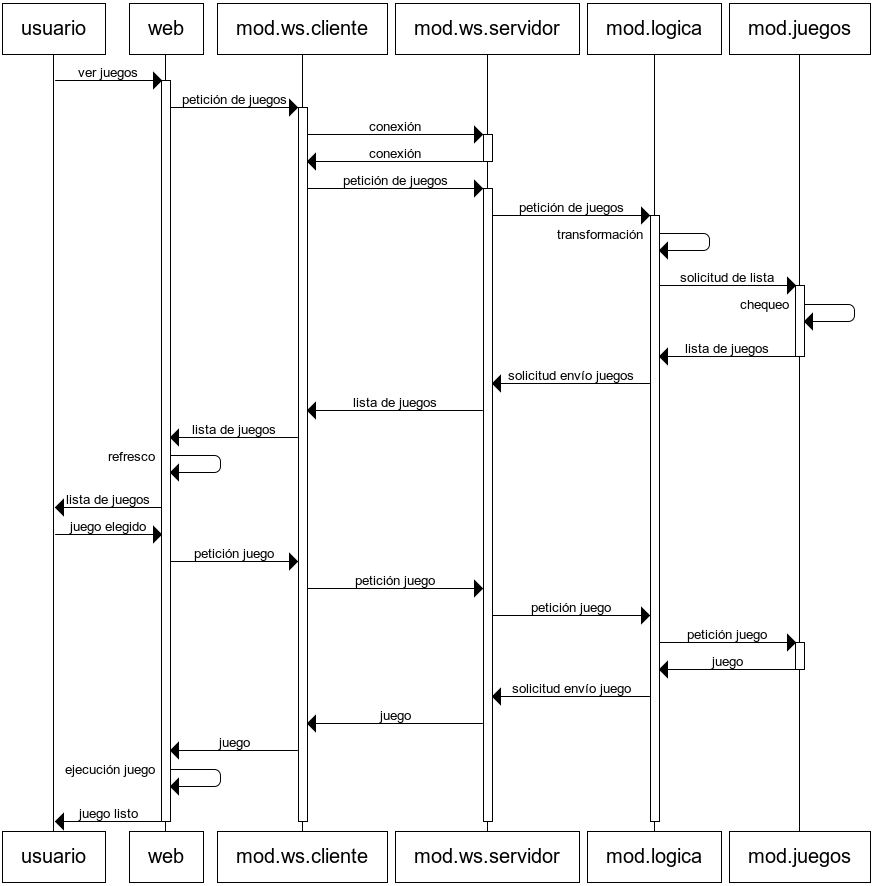
\includegraphics[width=\textwidth]{images/uc-12.png}
      \caption{Diagrama de interacción del caso de uso UC-12 (flujo normal)}
      \label{fig::uc-12}
    \end{center}
  \end{figure}
  


\item %%%%%%%%%%%%%%%%%%%%%%%%%%%%%%%%%%%%%%%%%%%%%%%%%%
  \begin{itemize}
  \item \textbf{Caso de uso}: Actualizar perfil cerebral
  \item \textbf{Requisitos funcionales asociados}: RF-8, RF-27
  \item \textbf{Actores}
    \begin{itemize}
    \item SGBD
    \end{itemize}
  \item \textbf{Descripción}: Tras una partida, el perfil cerebral es actualizado.
  \item \textbf{Precondiciones}
    \begin{itemize}
    \item El usuario está autenticado en el sistema.
    \item El usuario acaba de terminar una partida.
    \end{itemize}
  \item \textbf{Postcondiciones}
    \begin{itemize}
    \item El perfil cerebral del usuario queda modificado.
    \end{itemize}
  \item \textbf{Flujo normal}
    \begin{enumerate}
    \item La web solicita el envío del resultado al módulo cliente de websockets.
    \item El módulo cliente de websockets envía el resultado al módulo servidor de websockets.
    \item El módulo servidor de websockets pasa el resultado al módulo de lógica del servidor.
    \item El módulo de lógica solicita la actualización del perfil cerebral al módulo de persistencia.
    \item El módulo de persistencia ejecuta las consultas de actualización sobre el SGBD.
    \item El SGBD realiza la actualización del perfil cerebral y devuelve una confirmación al módulo de persistencia.
    \item El módulo de persistencia devuelve la confirmación al módulo de lógica.
    \item El módulo de lógica solicita el envío de la confirmación al módulo servidor de websockets.
    \item El módulo servidor de websockets envía la confirmación al módulo cliente de websockets.
    \item El módulo cliente de websockets pasa la confirmación a la web.
    \item La web muestra una notificación confirmando que el perfil cerebral ha sido actualizado.
    \end{enumerate}
  \item \textbf{Includes}
    \begin{itemize}
    \item Ninguno
    \end{itemize}
  \item \textbf{Extensiones}
    \begin{itemize}
    \item Ninguna
    \end{itemize}
  \end{itemize}

\item %%%%%%%%%%%%%%%%%%%%%%%%%%%%%%%%%%%%%%%%%%%%%%%%%%
  \begin{itemize}
  \item \textbf{Caso de uso}: Jugar a un juego monojugador
  \item \textbf{Requisitos funcionales asociados}: RF-8, RF-27
  \item \textbf{Actores}
    \begin{itemize}
    \item Usuario
    \item SGBD
    \end{itemize}
  \item \textbf{Descripción}: 
  \item \textbf{Precondiciones}
    \begin{itemize}
    \item El usuario debe estar autenticado en el sistema
    \item El usuario debe estar situado en la página de juegos, con el listado cargado.
    \end{itemize}
  \item \textbf{Postcondiciones}
    \begin{itemize}
    \item Ninguna
    \end{itemize}
  \item \textbf{Flujo normal}
    \begin{enumerate}
    \item El usuario selecciona un juego monojugador al que jugar.
    \item La web solicita el juego al módulo cliente de websockets.
    \item El módulo cliente de websockets envía la petición al módulo servidor de websockets.
    \item El módulo servidor de websockets pasa la petición al módulo de lógica.
    \item El módulo de lógica solicita el juego pedido al módulo de juegos.
    \item El módulo de juegos devuelve el juego solicitado completo.
    \item El módulo de lógica solicita el envío del juego al módulo servidor de websockets.
    \item El módulo servidor de websockets envía el juego al módulo cliente de websockets.
    \item El módulo cliente de websockets pasa el juego a la web.
    \item La web carga el juego recibido y lo ejecuta.
    \end{enumerate}
  \item \textbf{Includes}
    \begin{itemize}
    \item Ninguno
    \end{itemize}
  \item \textbf{Extensiones}
    \begin{itemize}
    \item UC-15
    \end{itemize}
  \item \textbf{Generalización de}: UC-12
  \end{itemize}

\item %%%%%%%%%%%%%%%%%%%%%%%%%%%%%%%%%%%%%%%%%%%%%%%%%%
  \begin{itemize}
  \item \textbf{Caso de uso}: Recomendar juego
  \item \textbf{Requisitos funcionales asociados}: RF-8, RF-27, RF-25
  \item \textbf{Actores}
    \begin{itemize}
    \item Usuario
    \item SGBD
    \end{itemize}
  \item \textbf{Descripción}: El usuario recomienda un juego monojugador a otro usuario.
  \item \textbf{Precondiciones}
    \begin{itemize}
    \item El usuario está autenticado en el sistema.
    \item El usuario ha cargado un juego.
    \end{itemize}
  \item \textbf{Postcondiciones}
    \begin{itemize}
    \item El usuario destino de la recomendación recibe una notificación por email.
    \end{itemize}
  \item \textbf{Flujo normal}
    \begin{enumerate}
    \item El usuario pulsa el botón de ``recomendar'' junto a un juego cargado, y selecciona un usuario al que enviar dicha recomendación.
    \item La web solicita el envío de la recomendación al módulo cliente de websockets.
    \item El módulo cliente de websockets envía la petición de recomendación al módulo servidor de websockets.
    \item El módulo servidor de websockets pasa la petición de recomendación al módulo de lógica.
    \item El módulo de lógica solicita los datos de contacto del usuario destino de la recomendación al módulo de persistencia.
    \item El módulo de persistencia realiza una consulta para recuperar la información del usuario destino de la recomendación al SGBD.
    \item El SGBD recupera la información y la envía de vuelta al módulo de persistencia.
    \item El módulo de persistencia pasa los datos de contacto al módulo de lógica.
    \item El módulo de lógica solicita el envío de la recomendación al módulo de email.
    \item El módulo de email envía la recomendación al usuario correspondiente, y devuelve una confirmación al módulo de lógica.
    \item El módulo de lógica solicita el envío de la confirmación de vuelta al cliente al módulo servidor de websockets.
    \item El módulo servidor de websockets envía la confirmación de recomendación al módulo cliente de websockets.
    \item El módulo cliente de websockets pasa la confirmación a la web.
    \item La web muestra una notificación informando de que la recomendación ha sido enviada correctamente.
    \end{enumerate}
  \item \textbf{Includes}
    \begin{itemize}
    \item Ninguno
    \end{itemize}
  \item \textbf{Extensiones}
    \begin{itemize}
    \item Ninguna
    \end{itemize}
  \end{itemize}


\item %%%%%%%%%%%%%%%%%%%%%%%%%%%%%%%%%%%%%%%%%%%%%%%%%%
  \begin{itemize}
  \item \textbf{Caso de uso}: Jugar a un juego multijugador
  \item \textbf{Requisitos funcionales asociados}: RF-8, RF-27
  \item \textbf{Actores}
    \begin{itemize}
    \item Usuario
    \item SGBD
    \end{itemize}
  \item \textbf{Descripción}: 
  \item \textbf{Precondiciones}
    \begin{itemize}
    \item El usuario debe estar autenticado en el sistema.
    \item El usuario debe estar situado en la página de juegos, con el listado cargado.
    \end{itemize}
  \item \textbf{Postcondiciones}
    \begin{itemize}
    \item El perfil cerebral de ambos jugadores se ve modificado.
    \end{itemize}
  \item \textbf{Flujo normal}
    \begin{enumerate}
    \item El usuario selecciona un juego multijugador al que jugar y un usuario contra el que jugar.
    \item La web solicita el juego y el envío de la invitación al módulo cliente de websockets.
    \item El módulo cliente de websockets envía la petición al módulo servidor de websockets.
    \item El módulo servidor de websockets pasa la petición al módulo de lógica.
    \item El módulo de lógica solicita el envío de la invitación al módulo servidor de websockets.
    \item El módulo servidor de websockets envía la invitación al módulo cliente de websockets del otro usuario (el retado).
    \item El módulo cliente de websockets del usuario retado pasa la invitación a la web.
    \item La web muestra la invitación y permite aceptarla o rechazarla.
    \item El usuario retado acepta la invitación.
    \item La web envía el mensaje de aceptación al módulo cliente de websockets.
    \item El módulo cliente de websockets  del usuario retado envía el mensaje de aceptación al módulo servidor de websockets.
    \item El módulo servidor de websockets pasa el mensaje de aceptación al módulo de lógica.
    \item El módulo de lógica solicita el juego pedido al módulo de juegos.
    \item El módulo de juegos devuelve el juego solicitado completo.
    \item El módulo de lógica solicita el envío del juego al módulo servidor de websockets.
    \item El módulo servidor de websockets envía el juego al módulo cliente de websockets de cada usuario.
    \item El módulo cliente de websockets pasa el juego a la web.
    \item La web carga el juego recibido y lo ejecuta.    
    \end{enumerate}
  \item \textbf{Flujo alternativo 1}: El usuario retado rechaza la invitación a jugar
    \begin{enumerate}
    \item El usuario selecciona un juego multijugador al que jugar y un usuario contra el que jugar.
    \item La web solicita el juego y el envío de la invitación al módulo cliente de websockets.
    \item El módulo cliente de websockets envía la petición al módulo servidor de websockets.
    \item El módulo servidor de websockets pasa la petición al módulo de lógica.
    \item El módulo de lógica solicita el envío de la invitación al módulo servidor de websockets.
    \item El módulo servidor de websockets envía la invitación al módulo cliente de websockets del otro usuario (el retado).
    \item El módulo cliente de websockets del usuario retado pasa la invitación a la web.
    \item La web muestra la invitación y permite aceptarla o rechazarla.
    \item El usuario retado rechaza la invitación.
    \item La web envía el mensaje de rechazo al módulo cliente de websockets.
    \item El módulo cliente de websockets del usuario retado envía el mensaje de rechazo al módulo servidor de websockets.
    \item El módulo servidor de websockets pasa el mensaje de rechazo al módulo de lógica.
    \item El módulo de lógica solicita el envío de rechazo al módulo servidor de websockets.
    \item El módulo servidor de websockets envía el rechazo al módulo cliente de websockets del usuario original.
    \item El módulo cliente de websockets pasa el mensaje de rechazo a la web.
    \item La web notifica el rechazo del reto.
    \end{enumerate}
  \item \textbf{Includes}
    \begin{itemize}
    \item Ninguno
    \end{itemize}
  \item \textbf{Extensiones}
    \begin{itemize}
    \item UC-18
    \item UC-19
    \end{itemize}
  \item \textbf{Generalización de}: UC-12
  \end{itemize}


\item %%%%%%%%%%%%%%%%%%%%%%%%%%%%%%%%%%%%%%%%%%%%%%%%%%
  \begin{itemize}
  \item \textbf{Caso de uso}: Ver recomendaciones de juegos
  \item \textbf{Requisitos funcionales asociados}: RF-8, RF-27, RF-25
  \item \textbf{Actores}
    \begin{itemize}
    \item Usuario
    \item SGBD
    \end{itemize}
  \item \textbf{Descripción}: El usuario recibe recomendaciones automatizadas de juegos por parte del sistema de recomendación.
  \item \textbf{Precondiciones}
    \begin{itemize}
    \item El usuario está autenticado en el sistema.
    \end{itemize}
  \item \textbf{Postcondiciones}
    \begin{itemize}
    \item Ninguna
    \end{itemize}
  \item \textbf{Flujo normal}
    \begin{enumerate}
    \item El usuario accede a la página de juegos.
    \item La web solicita la recomendación de juegos al módulo cliente de websockets.
    \item El módulo cliente de websockets envía la petición al módulo servidor de websockets.
    \item El módulo servidor de websockets pasa la petición de recomendación al módulo de lógica.
    \item El módulo de lógica solicita el listado de juegos al módulo de juegos.
    \item El módulo de juegos devuelve al módulo de lógica el listado de juegos disponibles.
    \item El módulo de lógica solicita la información completa del usuario al módulo de persistencia.
    \item El módulo de persistencia lanza una consulta al SGBD para recuperar la información del usuario.
    \item El SGBD devuelve la información completa del usuario al módulo de persistencia.
    \item El módulo de persistencia pasa los datos del usuario al módulo de lógica.
    \item El módulo de lógica solicita la recomendación de juegos al módulo de recomendación, adjuntándole el listado de juegos y la información completa del usuario.
    \item El módulo de recomendación devuelve el resultado del algoritmo de recomendación de juegos al módulo de lógica.
    \item El módulo de lógica solicita el envío de la recomendación al módulo servidor de websockets.
    \item El módulo servidor de websockets envía la recomendación al módulo cliente de websockets.
    \item El módulo cliente de websockets pasa la recomendación a la web.
    \item La web muestra los resultados de la recomendación en la página de juegos.
    \end{enumerate}
  \item \textbf{Includes}
    \begin{itemize}
    \item Ninguno
    \end{itemize}
  \item \textbf{Extensiones}
    \begin{itemize}
    \item Ninguna
    \end{itemize}
  \end{itemize}

% \item %%%%%%%%%%%%%%%%%%%%%%%%%%%%%%%%%%%%%%%%%%%%%%%%%%
%   \begin{itemize}
%   \item \textbf{Caso de uso}: Retar a otro usuario
%   \item \textbf{Requisitos funcionales asociados}: RF-8, RF-27, RF-28
%   \item \textbf{Actores}
%     \begin{itemize}
%     \item Usuario
%     \item SGBD
%     \end{itemize}
%   \item \textbf{Descripción}: 
%   \item \textbf{Precondiciones}
%     \begin{itemize}
%     \item 
%     \end{itemize}
%   \item \textbf{Postcondiciones}
%     \begin{itemize}
%     \item 
%     \end{itemize}
%   \item \textbf{Flujo normal}
%     \begin{enumerate}
%     \item 
%     \end{enumerate}
%   \item \textbf{Includes}
%     \begin{itemize}
%     \item Ninguno
%     \end{itemize}
%   \item \textbf{Extensiones}
%     \begin{itemize}
%     \item Ninguna
%     \end{itemize}
%   \item \textbf{Diagrama de interacción}: Figura 
%   \end{itemize}


% \item %%%%%%%%%%%%%%%%%%%%%%%%%%%%%%%%%%%%%%%%%%%%%%%%%%
%   \begin{itemize}
%   \item \textbf{Caso de uso}: Aceptar reto de juego
%   \item \textbf{Requisitos funcionales asociados}: RF-8, RF-27, RF-28
%   \item \textbf{Actores}
%     \begin{itemize}
%     \item Usuario
%     \item SGBD
%     \end{itemize}
%   \item \textbf{Descripción}: 
%   \item \textbf{Precondiciones}
%     \begin{itemize}
%     \item 
%     \end{itemize}
%   \item \textbf{Postcondiciones}
%     \begin{itemize}
%     \item 
%     \end{itemize}
%   \item \textbf{Flujo normal}
%     \begin{enumerate}
%     \item 
%     \end{enumerate}
%   \item \textbf{Includes}
%     \begin{itemize}
%     \item Ninguno
%     \end{itemize}
%   \item \textbf{Extensiones}
%     \begin{itemize}
%     \item Ninguna
%     \end{itemize}
%   \item \textbf{Diagrama de interacción}: Figura 
%   \end{itemize}

\item %%%%%%%%%%%%%%%%%%%%%%%%%%%%%%%%%%%%%%%%%%%%%%%%%%
  \begin{itemize}
  \item \textbf{Caso de uso}: Ver recomendaciones de usuarios
  \item \textbf{Requisitos funcionales asociados}: RF-26
  \item \textbf{Actores}
    \begin{itemize}
    \item Usuario
    \item SGBD
    \end{itemize}
  \item \textbf{Descripción}: El usuario recibe recomendaciones automatizadas de usuarios similares a él por parte del sistema de recomendación.
  \item \textbf{Precondiciones}
    \begin{itemize}
    \item El usuario está autenticado en el sistema.
    \end{itemize}
  \item \textbf{Postcondiciones}
    \begin{itemize}
    \item Ninguna
    \end{itemize}
  \item \textbf{Flujo normal}
    \begin{enumerate}
    \item El usuario accede a la página de exploración de usuarios.
    \item La web solicita la recomendación de usuarios al módulo cliente de websockets.
    \item El módulo cliente de websockets envía la petición al módulo servidor de websockets.
    \item El módulo servidor de websockets pasa la petición de recomendación al módulo de lógica.
    \item El módulo de lógica solicita el listado de usuarios al módulo de persistencia.
    \item El módulo de persistencia lanza una consulta de usuarios al SGBD.
    \item El SGBD devuelve un listado acotado de usuarios.
    \item El módulo de persistencia devuelve al módulo de lógica el listado de usuarios.
    \item El módulo de lógica solicita la información completa del usuario al módulo de persistencia.
    \item El módulo de persistencia lanza una consulta al SGBD para recuperar la información del usuario.
    \item El SGBD devuelve la información completa del usuario al módulo de persistencia.
    \item El módulo de persistencia pasa los datos del usuario al módulo de lógica.
    \item El módulo de lógica solicita la recomendación de usuarios al módulo de recomendación, adjuntándole el listado de usuarios y la información completa del usuario.
    \item El módulo de recomendación devuelve el resultado del algoritmo de recomendación de usuarios al módulo de lógica.
    \item El módulo de lógica solicita el envío de la recomendación al módulo servidor de websockets.
    \item El módulo servidor de websockets envía la recomendación al módulo cliente de websockets.
    \item El módulo cliente de websockets pasa la recomendación a la web.
    \item La web muestra los resultados de la recomendación en la página de usuarios.
    \end{enumerate}
  \item \textbf{Includes}
    \begin{itemize}
    \item Ninguno
    \end{itemize}
  \item \textbf{Extensiones}
    \begin{itemize}
    \item Ninguna
    \end{itemize}
  \end{itemize}








\end{enumerate}






\section{Diseño}

Dada la naturaleza de la tecnología empleada para el desarrollo del sistema de BreakBrain, la implementación se lleva a cabo de forma modular sobre el núcleo que supone NodeJS\index{nodejs} ---en el lado del servidor---. Tanto a ese nivel como en el lado del cliente, se sigue el patrón MVC para la construcción del software.

En cuanto al servidor, las tres capas MVC son las siguientes:

\begin{itemize}
\item {\bf Servidor web / Servidor de websockets}: Se encarga de la comunicación con el sistema cliente. Actúa como intermediario entre éste y el núcleo del servidor, en el que se implementa la lógica principal del sistema.
\item {\bf Núcleo del servidor}: Se trata de la lógica de dominio, donde se codifica el comportamiento central de BreakBrain, en torno al cual se presentan el resto de componentes software.
\item {\bf Subsistema de persistencia}: Es el responsable del almacenamiento y recuperación de la información referida a los usuarios y las partidas, los perfiles de evolución cerebral, etc. Se comunica con el núcleo del servidor y actúa de intermediario entre éste y el \acf{SGBD}, que es proporcionado por un servicio remoto.
\end{itemize}

Atendiendo al cliente, las capas MVC en las que se divide su implementación son las enumeradas a continuación:

\begin{itemize}
\item {\bf Web (GUI)}: Se trata de la capa de presentación, a través de la cual el usuario interactúa con el sistema. Éste es el único componente software del cual el usuario final tiene constancia.
\item {\bf Lógica del cliente}: Esta capa manipula la información del usuario y actúa de intermediaria entre la interfaz gráfica (web) y la capa de persistencia temporal del cliente.
\item {\bf Persistencia temporal}: Se encarga de mantener la sesión temporal del usuario.
\end{itemize}

Cada módulo, así como cada capa, ofrece un acoplamiento mínimo con el resto, de tal forma que los cambios efectuados en cualquiera de ellos no afectan directamente a los demás. Por tanto, resulta sencilla la sustitución de módulos por nuevas versiones, por ejemplo, siempre y cuando se respete la interfaz de comunicación.

La figura \ref{fig::diseno} muestra de forma sencilla los componentes que constituyen el sistema, así como la conexión entre ellos. 

\section{Implementación}
\label{sec::implementacion}

La implementación de BreakBrain se ha llevado a cabo completamente desde cero, construyendo una red social completa sin emplear frameworks externos u otras facilidades. Las razones para hacerlo así son diversas, pero la más importante ha sido la voluntad de aprender cómo funciona hasta el más mínimo aspecto de un sistema tan grande y de estas características. Además se decidió apostar por tecnologías muy modernas y con buenos resultados.

En esta sección se presentan brevemente las tecnologías empleadas para implementar el sistema. Posteriormente se analiza la estructura del código fuente escrito, así como pequeñas estadísticas sobre el mismo.

\subsection{Tecnología}

A la hora de analizar las tecnologías empleadas en la construcción de BreakBrain, podemos realizar una sencilla clasificación por el ámbito en el cual han sido empleadas. Así pues, a continuación se detallan los lenguajes de programación, frameworks y entornos de ejecución utilizados por el sistema, y clasificados en tres grupos: servidor, cliente y comunicación.


\subsubsection{Tecnologías del servidor}

\begin{itemize}
\item {\bf JavaScript}: Es el lenguaje empleado para la implementación de todos los componentes del servidor.
\item {\bf NodeJS}: Entorno de ejecución de JavaScript basado en el motor V8 desarrollado por Google. Supone cierta revolución en el ámbito del desarrollo de aplicaciones web de tiempo real.
%\item {\bf Nodester}: \acf{PAAS} de hosting para aplicaciones web implementadas con NodeJS.
\item {\bf Express.js\index{express.js} \cite{Visionmedia}}: framework MVC para el desarrollo de aplicaciones web con NodeJS\index{nodejs}.
\item {\bf MongoDB}:Se trata de un motor de base de datos NoSQL de gran auge en la actualidad. Ofrece muy buenas estadísticas de rendimiento y escalabilidad.
%\item {\bf MongoLab}: \acf{SAAS} de bases de datos MongoDB.
%\item {\bf Amazon Web Storage}: \acf{SAAS} de almacenamiento en la nube.
\end{itemize}


\subsubsection{Tecnologías del cliente}

\begin{itemize}
\item {\bf HTML5}: Tecnología empleada para la construcción del documento estructurado que constituye la interfaz gráfica del cliente: la web.
\item {\bf CSS3}: Hojas de estilos para mejorar la apariencia y comportamiento de los documentos HTML.
\item {\bf JavaScript}: Lenguaje empleado para la implementación del comportamiento de la interfaz gráfica y de la lógica del cliente.
\end{itemize}

\subsubsection{Tecnologías de comunicación}

\begin{itemize}
\item {\bf Websockets}\index{websockets}: Tecnología que proporciona un canal de comunicación bidireccional y full-duplex sobre un único socket TCP. Está diseñada para ser implementada en navegadores y servidores web.
\end{itemize}


\subsection{Estructura del código fuente}

El código fuente está categorizado en dos grandes grupos: el código fuente del servidor y el código fuente del cliente. Dado que todos los lenguajes empleados en el desarrollo son interpretados, no es necesario pensar en procesos de compilación ni archivos binarios.

Para hacer uso de la web cliente, el usuario accede mediante su navegador web a la dirección donde se aloja BreakBrain. Además, las tecnologías empleadas para desarrollar el sistema son estándares soportados por todos los navegadores web modernos. Por tanto, no debemos preocuparnos por ningún tipo de proceso de instalación por parte del usuario. Así mismo, todos los ficheros fuente de BreakBrain se encuentran centralizados en el servidor, por lo que la actualización, corrección de errores, etc. resulta muy sencilla.

El código fuente se encuentra clasificado en la siguiente jerarquía de directorios:

\begin{verbatim}
/                        // Raíz del código. Servidor principal y tests
/node_modules/           // Módulos de terceros para NodeJS 
/server/                 // Módulos de BreakBrain para NodeJS
/server/games/           // Juegos de BreakBrain (parte del servidor)
/server/public/          // Contenido estático servido al cliente
/server/public/games/    // Juegos de BreakBrain (parte publica)
/server/public/js/       // Archivos JavaScript para la web del cliente
/server/public/css/      // Hojas de estilos para la web del cliente
/server/public/img/      // Imágenes servidas para la web del cliente
\end{verbatim}

En el cuadro \ref{tab::code} se ofrece una lista con los diferentes archivos fuente del sistema, junto a una descripción y una muestra de la extensión de cada uno.

\begin{table}
  \caption{Archivos de código fuente}
\label{tab::code}
  \begin{tabular}{lccl}
    \hline
    \tabheadformat
    Fichero fuente & Tipo & Num. de líneas & Descripción \\
    \hline
    {\tt /generator.js} & JavaScript & 67 & Generador de datos aleatorios \\
    {\tt /server.js} & JavaScript & 739 & Servidor principal \\
    {\tt /test.js} & JavaScript & 21 & Módulo de test unitarios \\
    {\tt /test-functionality.js} & JavaScript & 502 & Batería de tests funcionales \\
    {\tt /test-stress.js} & JavaScript & 63 & Batería de tests de estrés \\
    {\tt /server/constants.js} & JavaScript & 10 & Constantes del programa \\
    {\tt /server/database.js} & JavaScript & 56 & Módulo de persistencia \\
    {\tt /server/email.js} & JavaScript & 34 & Módulo de email \\
    {\tt /server/Game.js} & JavaScript & 65 & ``Clase'' padre de los juegos \\
    {\tt /server/games.js} & JavaScript & 43 & Módulo servidor de juegos \\
    {\tt /server/games/*} & JavaScript & 305 & Módulos servidores de los juegos \\
    {\tt /server/util.js} & JavaScript & 59 & Módulo de utilidades \\
    {\tt /public/games.html} & HTML & 56 & Vista de la página de juegos \\
    {\tt /public/header.html} & HTML & 18 & Vista de la cabecera \\
    {\tt /public/home.html} & HTML & 77 & Vista de la página de inicio \\
    {\tt /public/login.html} & HTML & 95 & Vista de la página de login \\
    {\tt /public/logout.html} & HTML & 13 & Vista de la página de logout \\
    {\tt /public/password.html} & HTML & 46 & Página de recuperación de contraseña \\
    {\tt /public/people.html} & HTML & 93 & Vista de la página ``gente'' \\
    {\tt /public/profile.html} & HTML & 171 & Vista de la página de perfil \\
    {\tt /public/css/*} & CSS & 1244 & Hojas de estilos del cliente \\
    {\tt /public/js/*} & JavaScript & 1646 & Archivos JavaScript del cliente \\
    \hline
  \end{tabular}

  
\end{table}


\section{Estadísticas del código fuente}

En el cuadro \ref{tab::stat} se muestra el nivel de utilización de cada lenguaje ---de programación o maquetación--- en la implementación de BreakBrain. Nótese la diferenciación entre JavaScript del lado del cliente y JavaScript del lado del servidor. Se ha realizado esta separación por la naturaleza clásica del desarrollo web de emplear dos lenguajes diferentes para el cliente y el servidor. En este caso se trata del mismo lenguaje, pero resulta de interés realizar una comparativa de la cantidad de código escrito en ambos extremos de la comunicación.

\begin{table}
  \caption{Estadísticas del código fuente de BreakBrain}
  \label{tab::stat}

  \begin{center}   
  \begin{tabular}{cccc}
    \hline
    \tabheadformat
    Lenguaje & Nº de archivos & Líneas de código & Protagonismo \\
    \hline
    JavaScript (cliente) & 15 & 1646 & 31.3\%\\
    JavaScript (servidor) & 13 & 1964 & 37.4\%\\
    HTML5 & 8 & 398 & 7.6\%\\
    CSS3 & 12 & 1244 & 23.7\%\\
    \hline
  \end{tabular}
  \end{center}
\end{table}


\begin{figure}[H]
  \begin{center}
    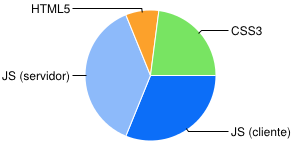
\includegraphics[scale=0.9]{./images/code-stats.png}
    % http://chart.apis.google.com/chart?chxs=0,030303,11.5&chxt=x&chs=300x150&cht=p&chco=0C6EF8|8DBAFA|FCA12B|78E462&chd=s:TXFO&chl=JS+(cliente)|JS+(servidor)|HTML5|CSS3
    \caption{Estadísticas del código fuente: los lenguajes de BreakBrain}
  \end{center}
\end{figure}


\section{Pruebas}

Con el fin de asegurar la calidad del software construido se han llevado a cabo diferentes tipos de pruebas sobre el mismo.

\subsection{Pruebas unitarias}

Para la realización de las pruebas unitarias se ha desarrollado un pequeño módulo ({\tt test.js}), que permite la realización de tests sencillos. Estos tests se han repartido por el código fuente en los puntos donde semánticamente tienen sentido, y sólo se lanzan si al ejecutar el servidor se le añade el argumento {\tt -t}. Al ejecutar el servidor de esta forma, el log muestra los casos de éxito y fracaso de todos los tests unitarios. Al finalizar los mismos se ofrece una pequeña estadística del resultado obtenido.

El subsistema de test tiene la particularidad de que posibilita su uso desde los nuevos juegos que se creen, ofreciendo así una manera sencilla de realizar tests unitarios desde la implementación del nuevo juego sin tener que utilizar otros módulos externos. La forma de llevar a cabo tests es muy sencilla:

\begin{verbatim}
test('descripción del test', 
      expresion_que_debe_ser_true, // por ejemplo: instancia != null
     'mensaje de error');
\end{verbatim}

El resultado de la ejecución de los tests unitarios básicos del sistema es la mostrada en la figura \ref{fig::unit}. Nótese que dicho resultado es el correspondiente al caso de ejecución más básico, en el que no se carga ningún juego, por lo que a medida que se carguen diferentes juegos dotados de tests, esta salida será mayor.

\begin{figure}[h]
  \begin{center}
    
    \begin{verbatim}
sgmonda@envy:~/projects/breakbrain $ node server.js -t
27 Nov 2012 19:24:30::UNIT TEST 1 CORRECT: constants module load
27 Nov 2012 19:24:30::DATABASE: Connecting to MongoDB database...
27 Nov 2012 19:24:30::UNIT TEST 2 CORRECT: mongodb module load
27 Nov 2012 19:24:30::UNIT TEST 3 CORRECT: database server creation
27 Nov 2012 19:24:30::UNIT TEST 4 CORRECT: database object creation
27 Nov 2012 19:24:30::UNIT TEST 5 CORRECT: database collection retrieval
27 Nov 2012 19:24:30::UNIT TEST 6 CORRECT: connection to mongo server
27 Nov 2012 19:24:30::UNIT TEST 7 CORRECT: connection to mongo db
27 Nov 2012 19:24:31::UNIT TEST 8 CORRECT: database connection opening
27 Nov 2012 19:24:32::UNIT TEST 9 CORRECT: database authentication
27 Nov 2012 19:24:32::DATABASE: Connected and authenticated successfully
27 Nov 2012 19:24:32::UNIT TEST 10 CORRECT: database object instantiation
27 Nov 2012 19:24:32::UNIT TEST 11 CORRECT: fs module load
27 Nov 2012 19:24:32::UNIT TEST 12 CORRECT: express module load
27 Nov 2012 19:24:32::UNIT TEST 13 CORRECT: http module load
27 Nov 2012 19:24:32::UNIT TEST 14 CORRECT: web app creation
27 Nov 2012 19:24:32::EMAIL-MODULE: Email subsystem ready to send emails
27 Nov 2012 19:24:32::UNIT TEST 15 CORRECT: email module load
27 Nov 2012 19:24:32::GAMES-MODULE: Loading games server...
27 Nov 2012 19:24:32::WEB SERVER: running on port 20661
27 Nov 2012 19:24:32::UNIT TEST 16 CORRECT: games directory reading
27 Nov 2012 19:24:32::UNIT TEST 17 CORRECT: games count
27 Nov 2012 19:24:32::GAMES-MODULE: Loading game "Un juego"...
27 Nov 2012 19:24:32::UNIT TEST 18 CORRECT: particular game load
27 Nov 2012 19:24:32::UNIT TEST 19 CORRECT: games module load
27 Nov 2012 19:24:32::UNIT TEST 20 CORRECT: websockets module load
27 Nov 2012 19:24:32::WEBSOCKETS SERVER: running on port 20661
27 Nov 2012 19:24:32::MAIN SERVER: The whole server is ready!

27 Nov 2012 19:24:32::CORRECT UNIT TESTS: 20 (100%)
^Csgmonda@envy:~/projects/breakbrain $ 

    \end{verbatim}

    \caption{Resultado parcial de tests unitarios}
    \label{fig::unit}
  \end{center}
\end{figure}


\subsection{Pruebas funcionales}

Se han llevado a cabo una serie de pruebas funcionales automatizadas, que cubren los aspectos más importantes de la funcionalidad especificada en los apartados \ref{sec::requisitos} y \ref{sec::casos}. Dada la naturaleza asíncrona y no bloqueante de la tecnología con la que ha sido desarrollado el servidor del proyecto, estas pruebas se lanzan y analizan de forma asíncrona. Para ello se ha utilizado un módulo de NodeJS\index{nodejs} llamado \emph{Vows} \cite{Maecki}\index{vows}.

Estas pruebas se encuentran en el archivo {\tt tests-functionality.js}, y pueden lanzarse sobre el intérprete de NodeJS\index{nodejs} una vez que el servidor está en ejecución. Los resultados de estas pruebas se muestran en la figura \ref{fig::vows}.

\begin{figure}[h]
  \begin{center}
    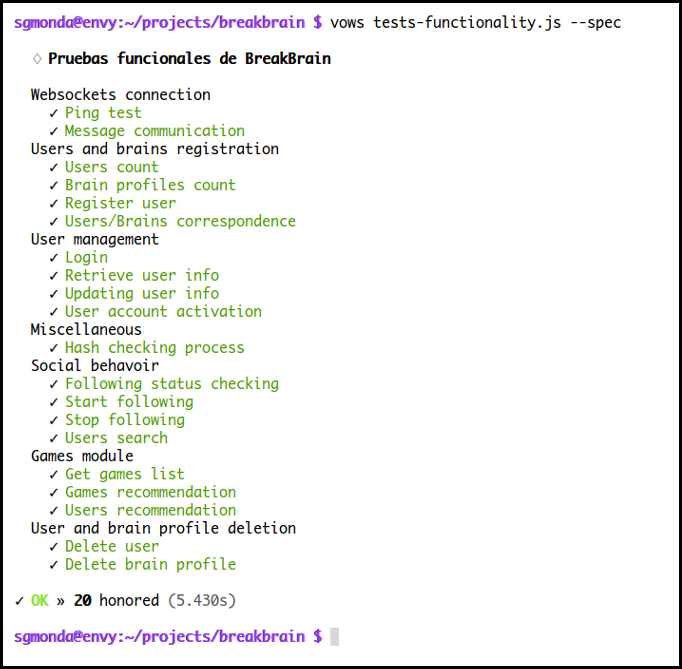
\includegraphics[width=0.8\textwidth]{images/vows.png}
    \caption{Resultados de la batería de tests funcionales}
    \label{fig::vows}
  \end{center}
\end{figure}



\subsection{Pruebas de aceptación}

Durante el desarrollo del sistema se han realizado pequeñas y repetidas pruebas de aceptación por parte de un subconjunto variado de usuarios finales, recogiendo las opiniones de los mismos y empleando éstas, junto con las estadísticas obtenidas, para la corrección de errores y mejora de aspectos varios.

La elección del subconjunto poblacional sometido a las pruebas de aceptación se ha llevado a cabo mediante un muestreo aleatorio estratificado, con el objetivo de obtener opiniones y observaciones de uso de usuarios de diferentes edades. Los estratos definidos para la realización del muestreo son los siguientes:

\begin{itemize}
\item Joven (entre 15 y 30 años de edad)
\item Adulto 1 (entre 30 y 45 años de edad)
\item Adulto 2 (entre 45 y 60 años de edad)
\end{itemize}

Durante la planificación de las pruebas se seleccionó aleatoriamente un individuo de cada subconjunto ---dichas personas se comprometieron a someterse a las pruebas de forma periódica---. Los individuos representantes de cada estrato son los siguientes:

\begin{itemize}
\item Joven - Rodrigo Testillano
\item Adulto 1 - Néstor Ceballos
\item Adulto 2 - Rafael García
\end{itemize}


En total se han llevado a cabo 3 sesiones de pruebas de aceptación. A continuación se enumeran las actividades en las que consistió cada una de ellas:

\renewcommand{\labelenumi}{\bf PA-\arabic{enumi}}
\renewcommand{\labelenumii}{\arabic{enumii}. }
\begin{enumerate}
\item La primera sesión consistió en:
  \begin{itemize}
  \item Crearse una cuenta en la red social.
  \item Autenticarse en el sistema.
  \item Cerrar la sesión.
  \item Tratar de acceder al sistema con datos erróneos.
  \item Simular el olvido de la contraseña para recuperar el acceso a su cuenta.
  \end{itemize}

\item La segunda sesión comprendió el uso de la red y la gestión de perfiles:
  \begin{enumerate}
  \item Explorar las estadísticas del perfil de usuario.
  \item Modificar la información personal del perfil.
  \item Modificar las preferencias de entrenamiento cerebral.
  \item Búsqueda de usuarios.
  \item Seguir y dejar de seguir a otros usuarios.
  \end{enumerate}

\item En la tercera sesión los individuos utilizaron el subsistema de juegos: 
  \begin{enumerate}
  \item Exploración de los juegos individuales.
  \item Exploración de los juegos multijugador.
  \item Jugar a un juego monojugador.
  \item Retar a otro usuario a un juego multijugador.
  \item Ser retado por otro usuario y aceptar. Jugar partida multijugador.
  \item Ser retado por otro usuario y rechazar la invitación.
  \end{enumerate}

\end{enumerate}

Los resultados obtenidos durante estas pruebas de aceptación fueron de gran utilidad, no sólo para solucionar ciertos problemas que no habían sido localizados hasta el momento de la utilización del sistema por parte del usuario final, sino también para mejorar la \emph{usabilidad}\index{usabilidad} ante problemas de diseño detectados durante la observación del uso por parte de los individuos. En resumen, algunos de los beneficios de estas pruebas fueron los siguientes:

\begin{itemize}
\item Corrección de pequeños errores de programación (\emph{bugs}\index{bug}).
\item Corrección de problemas de distribución de elementos en la web (problemas de usabilidad\index{usabilidad}).
\item Aceptación de críticas sobre los esquemas de color y rediseño de los mismos.
\item Mejora de la interacción hombre-máquina ante la observación de dificultades de uso de algunos componentes por parte de ciertos individuos.
\end{itemize}


\subsection{Pruebas de estrés del sistema}

Esta batería de pruebas permite observar el comportamiento y escalabilidad del sistema, observando el comportamiento del mismo en situaciones de poca carga y en situaciones extremas, con gran cantidad de peticiones costosas simultáneas.

Cabe añadir que la probabilidad de que el sistema se vea sometido a estas situaciones extremas en un entorno real es despreciable. Sin embargo, estas pruebas resultan de gran utilidad para estudiar la respuesta del servidor y la base de datos.

\begin{figure}[h]
  \begin{center}
    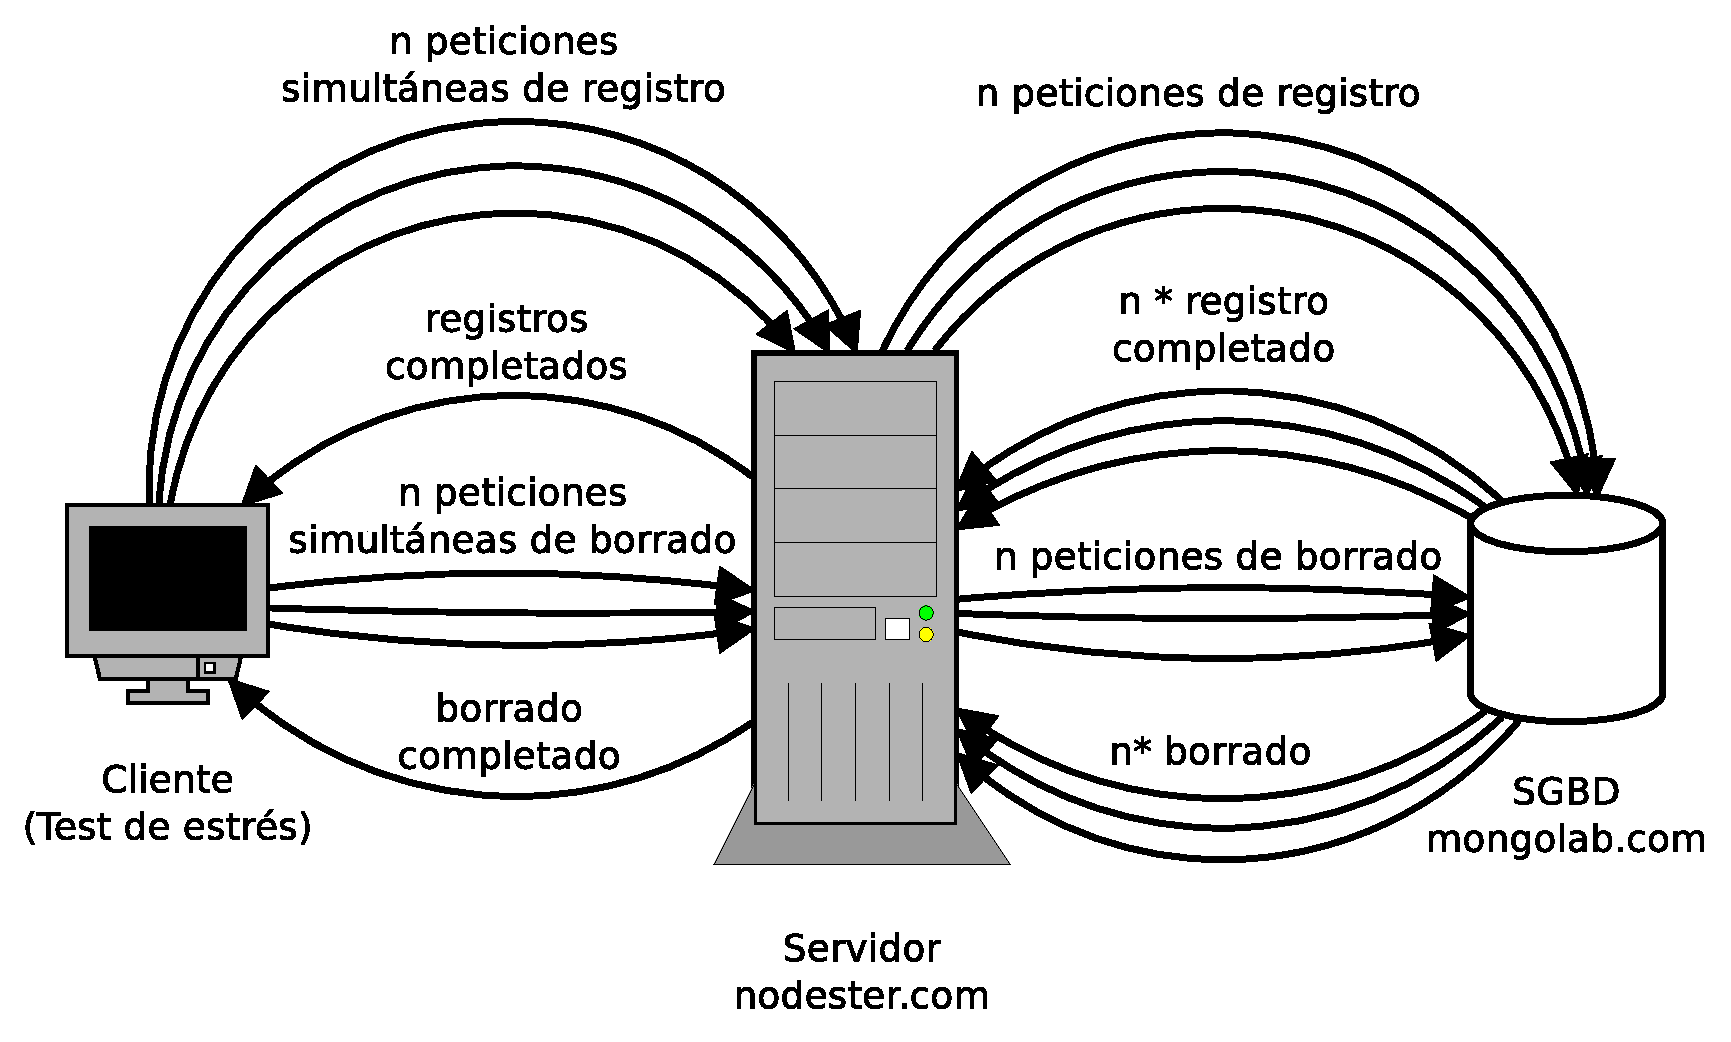
\includegraphics[width=\textwidth]{images/estres.eps}
    \caption{Diseño del test de estrés}
    \label{fig::estres}
  \end{center}
\end{figure}

Para realizar las pruebas de estrés se ha diseñado un pequeño programa que lanza peticiones simultáneas contra el servidor. Las peticiones lanzadas son de registro y borrado de usuarios. Se ha seleccionado la operación de registro de un usuario ---con generación aleatoria de datos--- porque es la que más coste tiene para la base de datos, y así nos permite abarcar toda la amplitud del sistema. Por otro lado, las operaciones de eliminación se han incluido en el test símplemente para eliminar los usuarios y perfiles cerebrales creados en la etapa anterior, y así servir también de contraste, al tratarse de la operación de menor coste de la base de datos.

Los resultados obtenidos son los siguientes:

\begin{itemize}
\item 1 única petición (RAM: 13MB)

  \begin{lstlisting}
STRESS-TEST: Starting stress test
STRESS-TEST: 1 false users registered
Time spent in 1 false users registration: 648ms
STRESS-TEST: False users deleted
STRESS-TEST: Stress test finished in 
Time spent in 1 false users deletion: 270ms
Time spent in whole stress test: 918ms
  \end{lstlisting}
  

\item 10 peticiones simultáneas (RAM: 15.7MB)
  \begin{lstlisting}
STRESS-TEST: Starting stress test
STRESS-TEST: 10 false users registered
Time spent in 10 false users registration: 964ms
STRESS-TEST: False users deleted
STRESS-TEST: Stress test finished in 
Time spent in 10 false users deletion: 272ms
Time spent in whole stress test: 1236ms
  \end{lstlisting}

\item 20 peticiones simultáneas (RAM: 17MB)
  \begin{lstlisting}
STRESS-TEST: Starting stress test
STRESS-TEST: 20 false users registered
Time spent in 20 false users registration: 469ms
STRESS-TEST: False users deleted
STRESS-TEST: Stress test finished in 
Time spent in 20 false users deletion: 277ms
Time spent in whole stress test: 748ms
  \end{lstlisting}

\item 50 peticiones simultáneas (RAM: 19MB)
  \begin{lstlisting}
STRESS-TEST: Starting stress test
STRESS-TEST: 50 false users registered
Time spent in 50 false users registration: 864ms
STRESS-TEST: False users deleted
STRESS-TEST: Stress test finished in 
Time spent in 50 false users deletion: 320ms
Time spent in whole stress test: 1186ms
  \end{lstlisting}

\item 100 peticiones simultáneas (RAM: 21.4MB)
  \begin{lstlisting}
STRESS-TEST: Starting stress test
STRESS-TEST: 100 false users registered
Time spent in 100 false users registration: 6955ms
STRESS-TEST: False users deleted
STRESS-TEST: Stress test finished in 
Time spent in 100 false users deletion: 1387ms
Time spent in whole stress test: 8342ms
  \end{lstlisting}

\item 200 peticiones simultáneas (RAM: 28.5MB)
  \begin{lstlisting}
STRESS-TEST: Starting stress test
STRESS-TEST: 200 false users registered
Time spent in 200 false users registration: 14460ms
STRESS-TEST: False users deleted
STRESS-TEST: Stress test finished in 
Time spent in 200 false users deletion: 1870ms
Time spent in whole stress test: 16330ms
  \end{lstlisting}

\item 500 peticiones simultáneas (RAM: 59MB)
  \begin{lstlisting}
STRESS-TEST: Starting stress test
STRESS-TEST: 500 false users registered
Time spent in 500 false users registration: 34901ms
STRESS-TEST: False users deleted
STRESS-TEST: Stress test finished in 
Time spent in 500 false users deletion: 5654ms
Time spent in whole stress test: 40555ms
  \end{lstlisting}

\item 1000 peticiones simultáneas (RAM: 128MB)
  \begin{lstlisting}
STRESS-TEST: Starting stress test
STRESS-TEST: 1000 false users registered
Time spent in 1000 false users registration: 65909ms
STRESS-TEST: False users deleted
STRESS-TEST: Stress test finished in 
Time spent in 1000 false users deletion: 14254ms
Time spent in whole stress test: 80163ms
  \end{lstlisting}

\item 5000 peticiones simultáneas (RAM: 340MB)
  \begin{lstlisting}
STRESS-TEST: Starting stress test
STRESS-TEST: 5000 false users registered
Time spent in 5000 false users registration: 322281ms
STRESS-TEST: False users deleted
STRESS-TEST: Stress test finished in 
Time spent in 5000 false users deletion: 75101ms
Time spent in whole stress test: 397382ms
  \end{lstlisting}

\item 10000 peticiones simultáneas (RAM: 520MB)
  \begin{lstlisting}
STRESS-TEST: Starting stress test
STRESS-TEST: 10000 false users registered
Time spent in 10000 false users registration: 547662ms
STRESS-TEST: False users deleted
STRESS-TEST: Stress test finished in 
Time spent in 10000 false users deletion: 229148ms
Time spent in whole stress test: 776810ms
  \end{lstlisting}

\end{itemize}

\begin{table}
  \caption{Estadísticas de las pruebas de estrés en un servidor Debian 64-bits Linux 3.2.0, CPU Intel Core i7 Q720 1.60GHz x 4, RAM 6GB}
  \begin{center}   
    \begin{tabular}{|c||c|c|c||c|}
      \hline
      \tabheadformat
      Peticiones & Tiempo total de & Tiempo total de & Tiempo total & Memoria RAM\\
     \tabheadformat
      simultáneas & inserciones & eliminaciones & del test & (server)\\
      \hline      \hline
      1 & 669 ms & 271 ms & 940 ms & 13 MB\\
      \hline
      10 & 964 ms & 272 & 1236 ms & 15.7 MB\\
      \hline
      20 & 469 ms & 277 ms & 748 ms & 17 MB\\
      \hline
      50 & 864 ms & 320 ms & 1186 ms & 19 MB\\
      \hline
      100 & 6955 ms & 1387 ms & 8342 ms & 21.4 MB\\
      \hline
      200 & 14460 ms & 1870 ms & 16330 ms & 28.5 MB\\
      \hline
      500 & 34901 ms & 5654 ms & 40555 ms & 50 MB\\
      \hline
      1000 & 65909 ms & 14254 ms & 80163 ms & 128 MB\\
      \hline
      5000 & 322281 ms & 75101 ms & 397382 ms & 340 MB\\
      \hline
      10000 & 547662 ms & 229148 ms & 776810 ms & 520 MB\\
      \hline
    \end{tabular}
  \end{center}
\end{table}


\begin{figure}[h]
  \begin{center}
    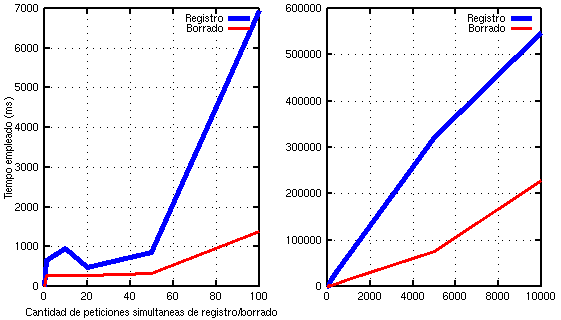
\includegraphics[width=\textwidth]{images/estresplot.png}
    \caption{Resultados de las pruebas de estrés}
    \label{fig::estres-plot}
  \end{center}
\end{figure}

A la vista de los resultados puede observarse el buen comportamiento del servidor para situaciones normales y extremas. Por supuesto, el caso de recibir gran cantidad de peticiones de registro simultáneas es muy poco probable, pero nos da una idea del rendimiento del sistema. El registro es la operación más costosa (para el subsistema de base de datos), y por ello ha sido elegida como \emph{operación estresante} para someter al sistema a ella.


% function drawVisualization() {
%   // Create and populate the data table.
%   var data = google.visualization.arrayToDataTable([
%     ['x', 'Registro', 'Borrado', 'RAM'],
%     ['0',   0,       0,           20.5],
%     ['1',   669,       271,         1],
%     ['10',   964,       272,           0.5],
%     ['20',   469,       277,         1],
%     ['50',   864,       320,           0.5],
%     ['100',   6955,       1387,         1],
%     ['200',   14460,       1870,           0.5],
%     ['500',   34901,       5654,         1],
%     ['1000',   65909,       14254,           0.5],
%     ['5000',   65909,       14254,           0.5],
%     ['10000',   65909,       14254,           0.5],
%     ['50000',   65909,       14254,           0.5]
%   ]);

%   // Create and draw the visualization.
%   new google.visualization.LineChart(document.getElementById('visualization')).
%       draw(data, {curveType: "function",
%                   width: 500, height: 400,
%                   vAxis: {maxValue: 10}}
%           );
% }
% ​




\chapter{Arquitectura}
\label{chap:arquitectura}

\drop{E}{ste} capítulo pretende ofrecer una visión completa de la composición del sistema informático que constituye BreakBrain, profundizando en los diferentes componentes que lo forman y haciendo hincapié en los patrones de diseño utilizados y otros detalles de interés para el lector con conocimientos técnicos.

A lo largo de las siguientes secciones, se presentará la arquitectura detallada del sistema completo, para después estudiar a más bajo nivel los componentes principales por separado, centrando la atención en el del desarrollo de software.

\section{Composición del sistema}

\begin{figure}[h]
  \begin{center}
    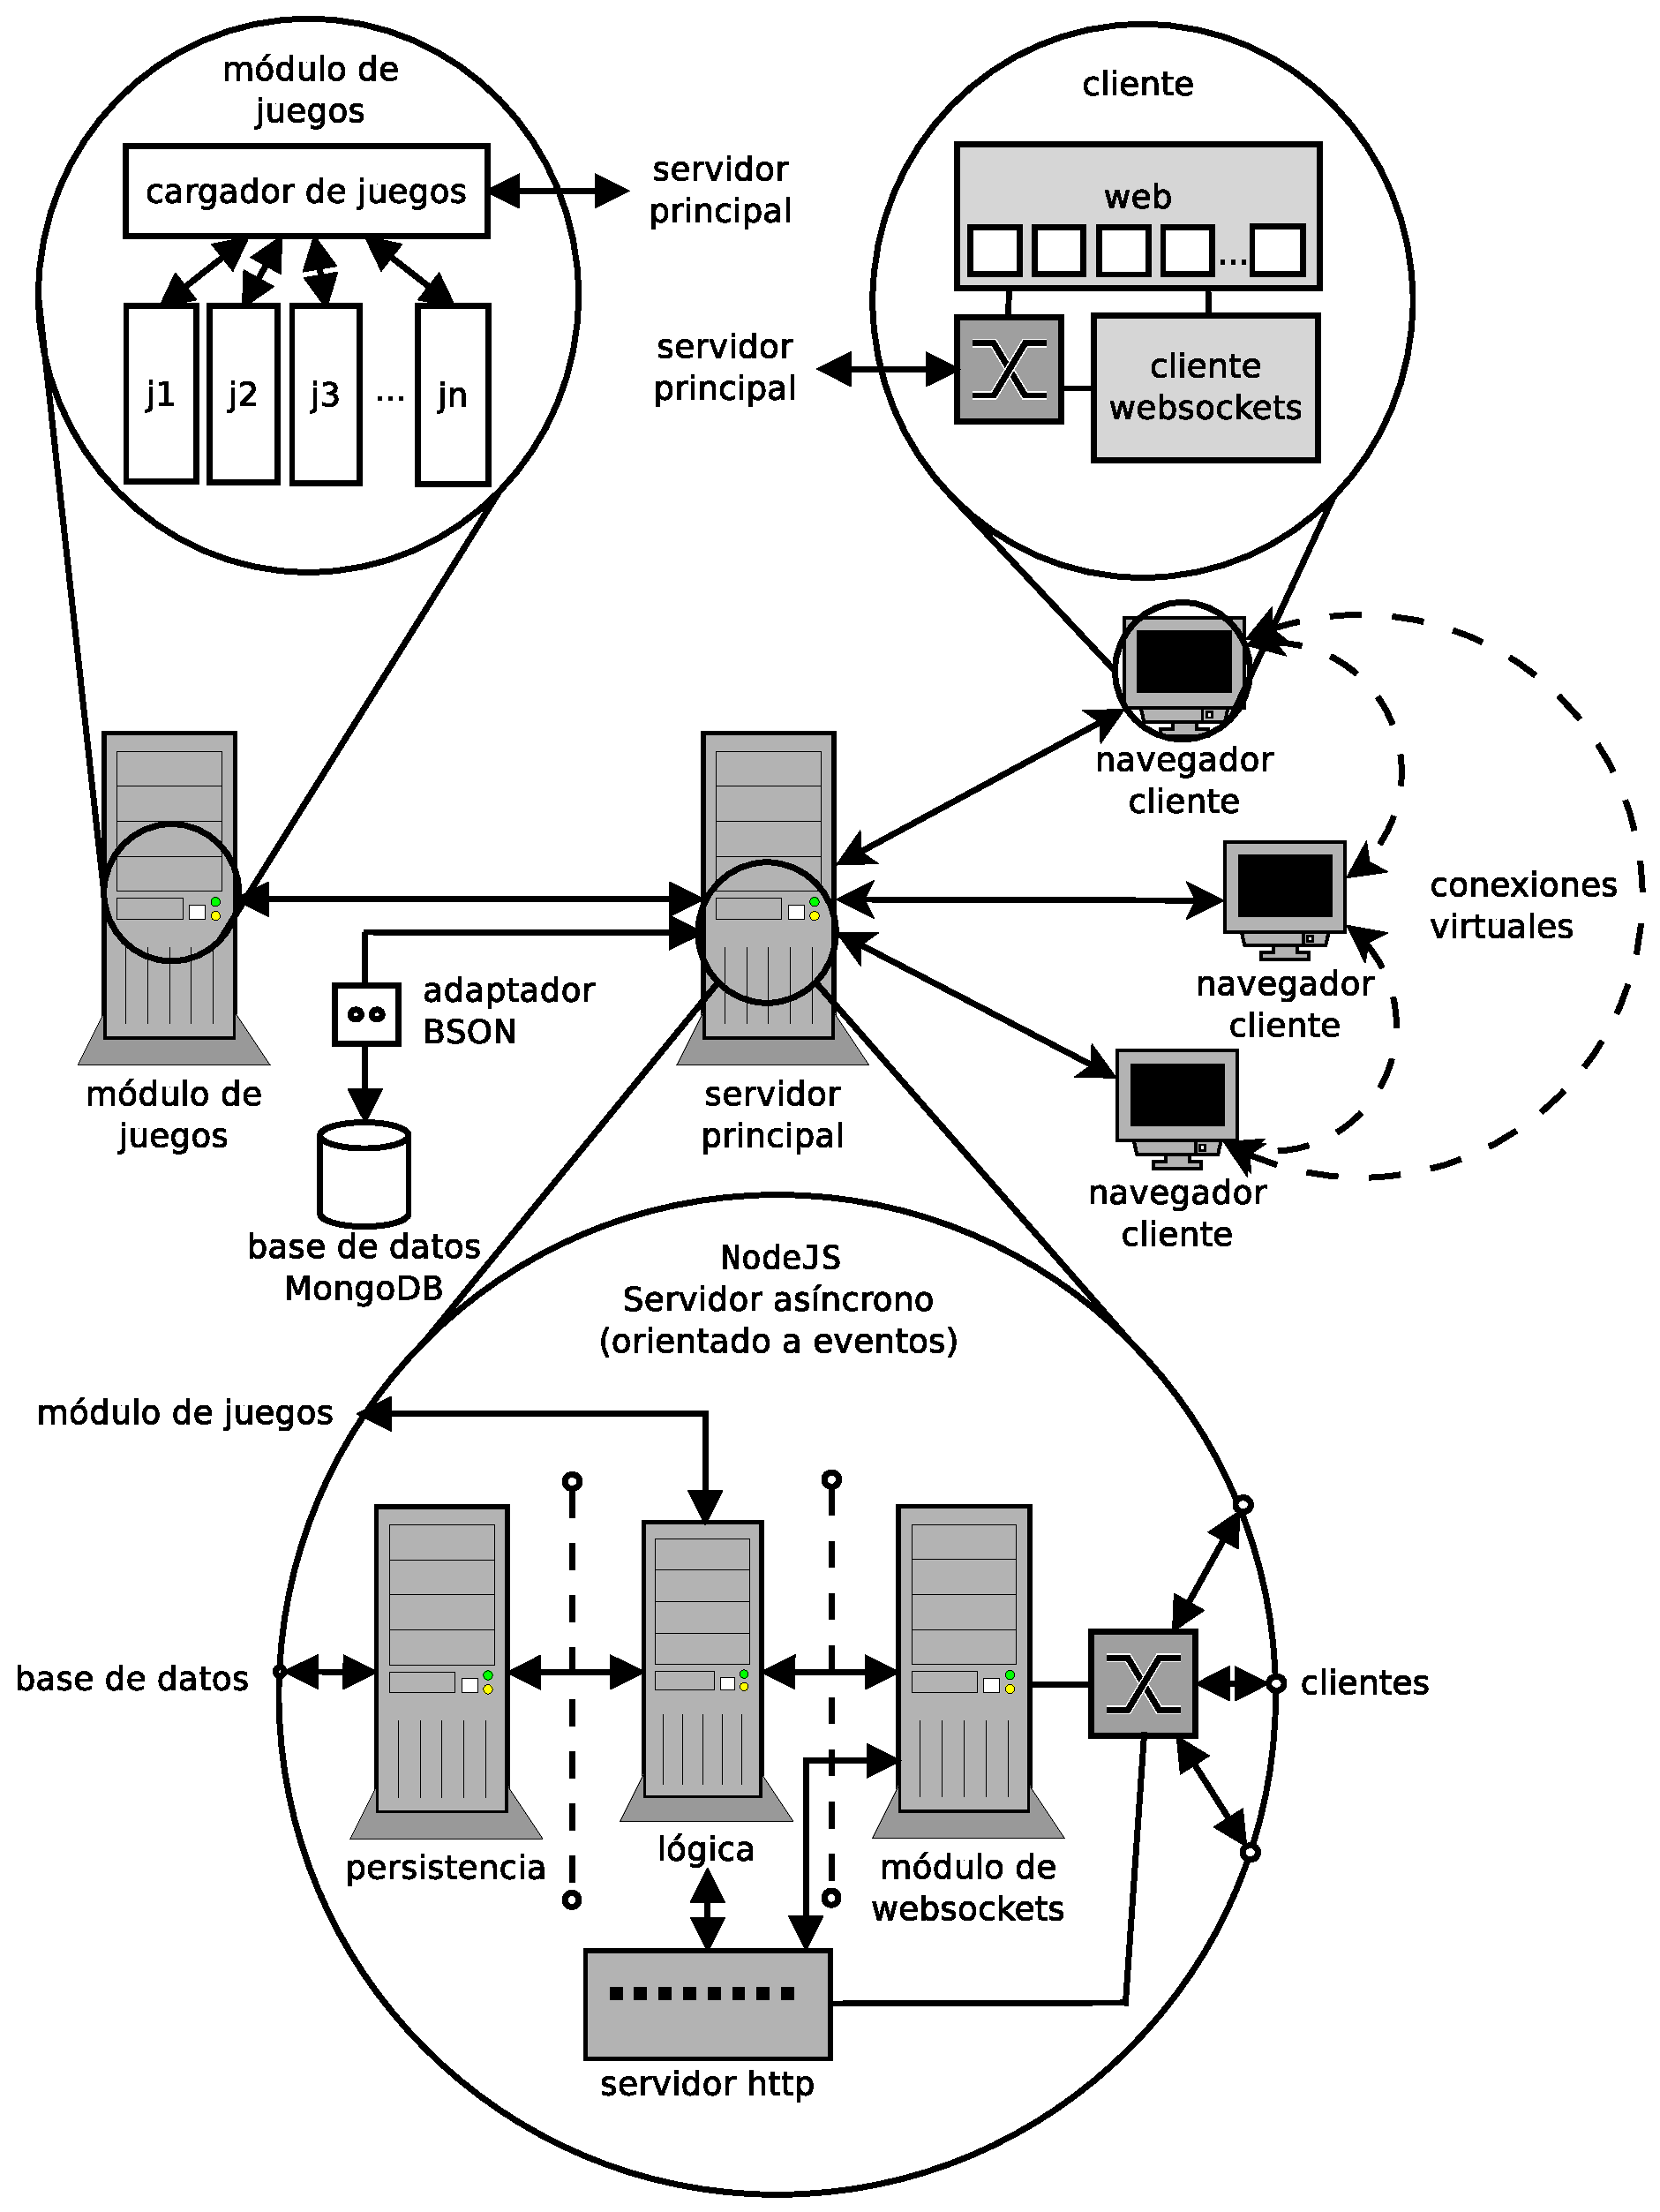
\includegraphics[width=\textwidth]{images/arquitectura.eps}
    \caption{Arquitectura detallada del sistema}
    \label{fig::arquitectura}
  \end{center}
\end{figure}

En la figura \ref{fig::arquitectura} se ofrece una visión detallada del los componentes que forman BreakBrain. Se trata de un enfoque de medio nivel que se adentra en la composición de los diferentes elementos de despliegue del sistema vistos en la sección \ref{sec::despliegue}. Como puede apreciarse, los dos protagonistas del enfoque {\it cliente-servidor} que sigue BreakBrain son tan complejos que se hace patente la necesidad de estudiarlos de forma detallada por separado.

A la vista de la figura \ref{fig::arquitectura} se perciben cuatro elementos esenciales en la composición del sistema:

\begin{itemize}
\item {\bf Cliente}\\Sitio web ejecutado sobre un navegador corriente. El uso de JavaScript que hace BreakBrain es intenso, tanto por la ejecución de los juegos como por el subsistema de comunicación permanente (necesario para los juegos multijugador), por lo que un navegador con buen soporte de JavaScript (como Chrome/Chromium \cite{chrome}) otorgará siempre una mejor experiencia de usuario.
\item {\bf Servidor principal}\\Se trata del corazón del sistema, compuesto principalmente por un servidor web corriente, al que se le ha añaido un servidor de comunicaciones mediante sockets TCP (con mensajes encapsulados en HTTP) para mantener una comunicación ininterrumpida con los clientes, y ofrecer así la base para la ejecución de juegos multijugador. El servidor se ejecuta en Nodester \cite{Nodester}, \acf{PAAS} de Software Libre que ofrece un buen servicio de forma totalmente gratuita.
\item {\bf Servidor de juegos}\\La piedra angular del servicio de juegos monojugador y multijugador. Construido de forma extensible, permite la integración de juegos de terceros en la plataforma. 
\item {\bf Sistema gestor de base de datos}\\Se ha optado por una base de datos no relacional MongoDB, alojada en los servicios de Amazon WS \cite{Amazon} y gestionada por MongoLab \cite{Mongolab}. Este último \acf{SAAS} se encarga del mantenimiento de la base de datos, asegurando la alta disponibilidad y escalabilidad.
\end{itemize}

\section{Arquitectura del sitio web}

La aplicación web de BreakBrain ha sido desarrollada utilizando NodeJS y ExpressJS, lo que fuerza la arquitectura de la misma hacia un enfoque \acf{MVC}. A su vez, la parte cliente (página web) ha sido desarrollada siguiendo este patrón.

\begin{figure}[H]
  \begin{center}
    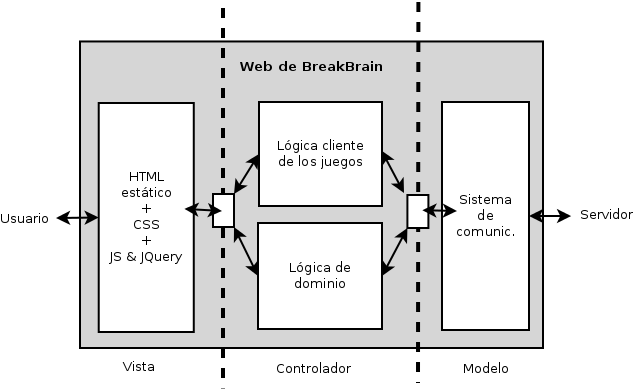
\includegraphics[width=\textwidth]{images/mvc-cliente.png}
    \caption{Patrón MVC en el cliente de BreakBrain}
    \label{fig::mvc-cliente}
  \end{center}
\end{figure}

\subsection{Patrón MVC}

La arquitectura Modelo-Vista-Controlador en el cliente de la plataforma se distingue atendiendo a la división de los componentes que la constituyen en los siguientes tres grupos:

\begin{itemize}
\item {\bf Modelo}: Sistema de comunicación con el servidor.

\item {\bf Vista}: Interfaz gráfica con la que el usuario interactúa. Se trata de código \acs{HTML} embellecido con estilos \acs{CSS} y manipulado mediante JavaScript, haciendo uso de JQuery.

\item {\bf Controlador}: Lógica principal del cliente. Aquí pueden distinguirse dos componentes principales:

  \begin{itemize}
  \item Lógica de dominio a nivel de cliente
  \item Lógica de la parte cliente de los juegos
  \end{itemize}
\end{itemize}

En la figura \ref{fig::mvc-cliente} se aprecia el esquema expuesto.

\section{Arquitectura del servidor}

La aplicación web de BreakBrain ha sido desarrollada utilizando NodeJS y ExpressJS, lo que fuerza la arquitectura de la misma hacia un enfoque \acf{MVC}. A su vez, la parte servidora ha sido desarrollada siguiendo este patrón.

\begin{figure}[H]
  \begin{center}
    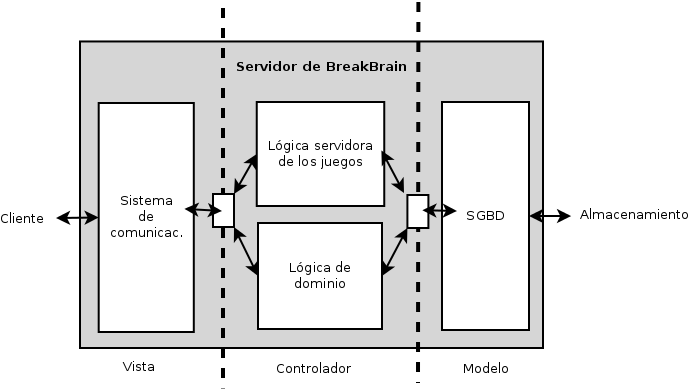
\includegraphics[width=\textwidth]{images/mvc-servidor.png}
    \caption{Patrón MVC en el servidor de BreakBrain}
    \label{fig::mvc-servidor}
  \end{center}
\end{figure}

\subsection{Patrón MVC}

La arquitectura Modelo-Vista-Controlador en el servidor de la plataforma se distingue atendiendo a la división de los componentes que la constituyen en los siguientes tres grupos:

\begin{itemize}
\item {\bf Modelo}: Subsistema de persistencia, encargado de la manipulación de la base de datos.
\item {\bf Vista}: Interfaz de comunicación con el cliente mediante websockets.
\item {\bf Controlador}: Lógica central del servidor, compuesta por dos subsistemas:

  \begin{itemize}
  \item Lógica de dominio a nivel de servidor
  \item Lógica de servidor de los juegos
  \end{itemize}
\end{itemize}

En la figura \ref{fig::mvc-servidor} se aprecia el esquema expuesto.

\section{Diseño modular}

La propia esencia de NodeJS, la tecnología con la que BreakBrain ha sido implementado, guía al desarrollador hacia una estructura basada en módulos independientes.

\vspace{0.1cm}
\begin{figure}[H]
  \begin{center}
    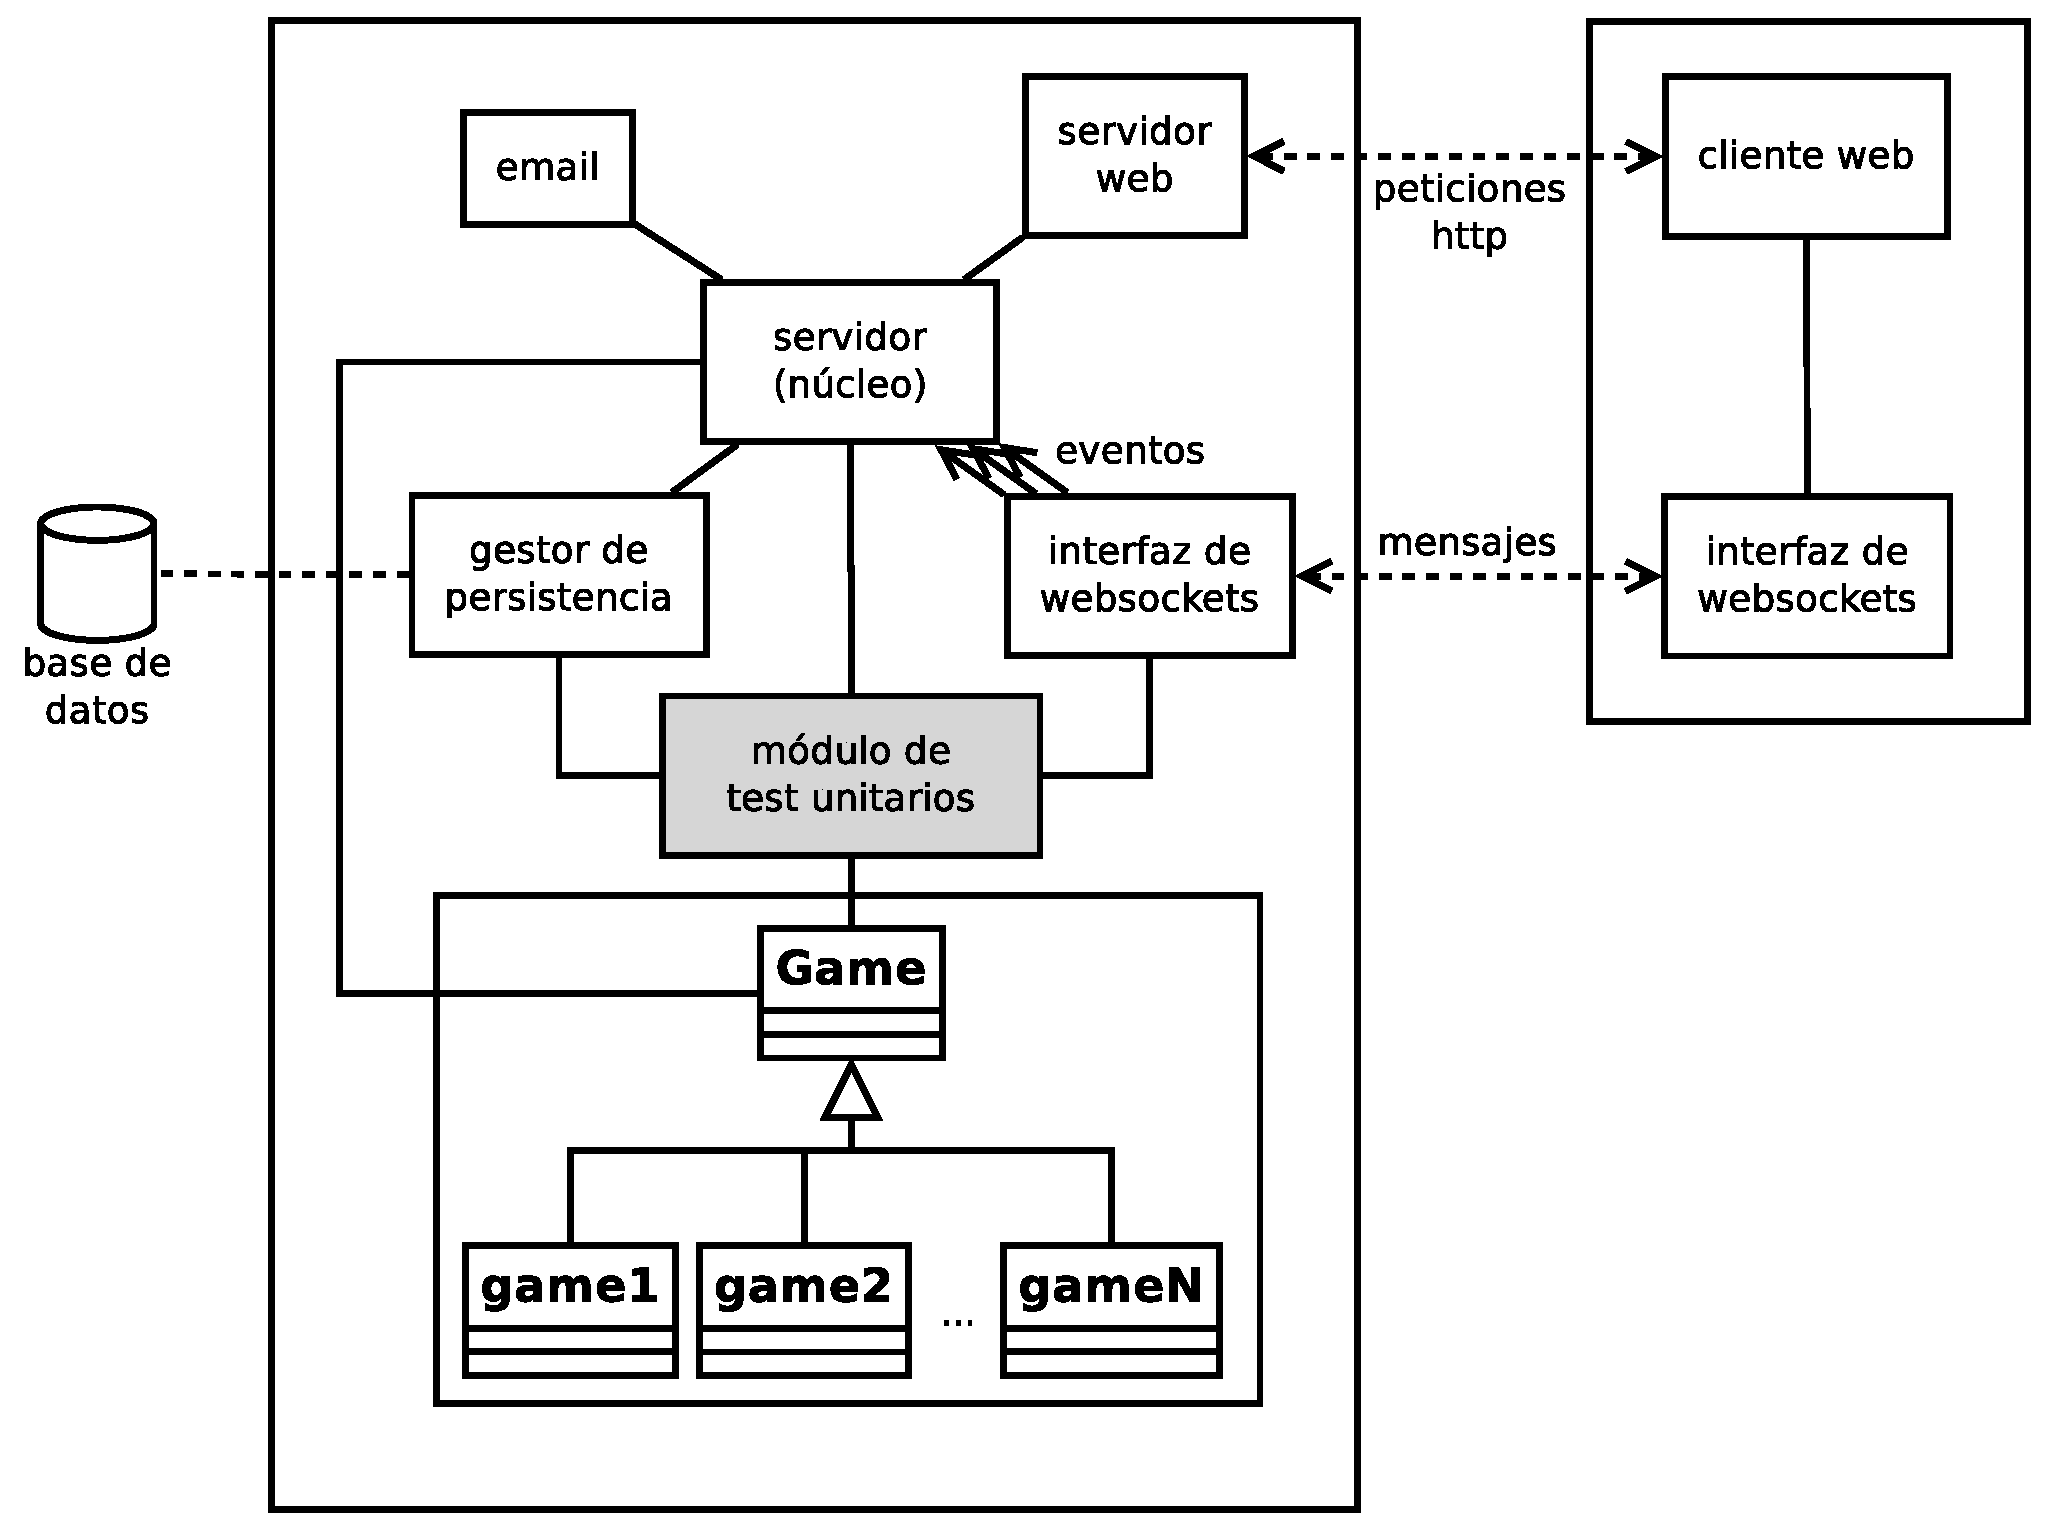
\includegraphics[width=\textwidth]{images/diseno.eps}
    \caption{Diseño modular del sistema}
    \label{fig::diseno}
  \end{center}
\end{figure}

En la figura \ref{fig::diseno} puede apreciarse la estructura modular de la plataforma, donde pueden distinguirse los siguientes componentes, agrupados según su funcionalidad:

\begin{itemize}
\item {\bf Gestor de persistencia}

Módulo encargado de la configuración y comunicación con el \acf{SGBD} utilizado (MongoDB).

\item {\bf Subsistema de email}

Módulo encargado del envío automático de emails.

\item {\bf Servidor web}

Módulo de manejo de peticiones y respuestas \acs{HTTP}, así como de la generación de contenido web dinámico para el cliente.

\item {\bf Servidor de websockets}

Módulo de conexión con el cliente mediante websockets. Mantiene (y pone a disposición de los juegos) una comunicación ininterrumpida con el navegador web de los usuarios.

\item {\bf Núcleo del servidor}

Módulo central, con la lógica de interconexión del resto de módulos y la creación de los propios servidores web y de websockets.

\item {\bf Módulo de test}

Módulo de pruebas de la plataforma.

\item {\bf Servidor de juegos}

Módulo encargado de la gestión de los juegos.

\item {\bf Cliente web}

El sitio web con el que el usuario interactúa.

\item {\bf Cliente de websockets}

Puente de comunicación entre el cliente y el servidor.

\end{itemize}





\chapter{Resultados}
\label{chap:resultados}

\drop{U}{na} vez adquiridos los conocimientos básicos sobre la estructura y funcionamiento del cerebro humano (sección \ref{sec::fisiologia}), así como sobre la neuroplasticidad\index{neuroplasticidad} (sección \ref{neuroplasticidad}) y el carácter maleable que ésta otorga al cerebro, en este capítulo se hace uso de esos conocimientos para la creación de un sistema de entrenamiento cerebral complejo. Además se ofrece una especificación detallada sobre cómo realizar una medición cuantitativa para poder valorar la evolución de dicho entrenamiento.

Por último se expondrán algunos algoritmos de recomendación que, haciendo uso de las métricas previamente definidas, permitirán encontrar usuarios afines a uno dado, así como juegos adecuados a un usuario en un instante concreto.

\section{Especificación del entrenamiento cerebral}
\label{sec:entrenamiento}
En base a la etapa de investigación documentada en las secciones \ref{sec::fisiologia} y \ref{neuroplasticidad}, las consideraciones que se han llevado a cabo para reconocer y diferenciar las capacidades mentales estimulables mediante el ejercicio agrupan estas capacidades en 5 grandes conjuntos:

\renewcommand{\labelenumi}{\bf\arabic{enumi}. }
\begin{enumerate}
\item Memoria
\item Resolución de problemas
\item Atención
\item Velocidad de procesamiento
\item Flexibilidad
\end{enumerate}

A continuación se presenta una jerarquía completa de las capacidades mentales consideradas, así como de las habilidades en que estas se han considerado subdivididas, detallándose el significado de cada una y cómo debe ser estimulada. En la figura \ref{fig::habilidades} se presenta un diagrama esquemático de dicha jerarquía.

\subsection{Memoria}

La mejora de la memoria se centra en tres aspectos realmente relevantes en la vida cotidiana: la memoria de trabajo, la memoria espacial y la memoria de asociación nombre-cara.

\begin{itemize}
\item {\bf Memoria de trabajo}

Procesos y estructuras de información empleados para el almacenamiento temporal y la manipulación de información durante el desarrollo de una tarea.

La memoria de trabajo requiere la activación de un circuito de neuronas, el cual activa en sí la memoria propiamente dicha. Esta memoria, si bien es activada desde la {\it corteza prefrontal}\index{córtex/corteza!prefrontal}, requiere a su vez la activación del resto de estructuras neuroanatómicas implicadas, como el \emph{lóbulo temporal}\index{lóbulo!temporal} para el significado o el \emph{lóbulo occipital}\index{lóbulo!occipital} para la imagen visual.

En un contexto informático, la memoria de trabajo se asemeja a la memoria RAM de un computador.

Los juegos para mejorar esta capacidad deben ofrecer pequeñas cantidades de información ---cada vez mayores según se aumente el nivel de dificultad--- durante un periodo corto de tiempo. El jugador debe asimilar esas porciones de información y recordarlas, para utilizarlas transcurrido un periodo de tiempo relativamente corto. El clásico juego de las parejas de cartas es un buen ejemplo. Otra posibilidad es ofrecer lecturas de párrafos cortos, y después jugar con esa información. Del mismo modo se puede jugar con otros sentidos, ofreciendo información auditiva, por ejemplo.

\item {\bf Memoria espacial}

Memoria responsable de registrar la información sobre el entorno y la orientación en el espacio.

Por ejemplo, en la vida real, la memoria espacial es la que nos permite recordar la ubicación del cuarto de baño de una casa ajena. De forma aún más sencilla, la memoria espacial nos permite trabajar en un escritorio, recordando dónde se encuentran los papeles, los lapiceros y bolígrafos, etc.

Los juegos dedicados al ejercicio y estimulación de esta capacidad mental deberán ofrecer un paisaje de objetos ---de complejidad variable, dependiendo de la dificultad de juego--- y dar un tiempo ---limitado o no--- para que el jugador memorice la localización de todos ellos. Después el jugador deberá reconstruir ese paisaje, de forma completa o parcial.

\item {\bf Memoria de asociación nombre-cara}

Se trata de los procesos relacionados con el registro y recuperación de la información que relaciona objetos visuales con objetos verbales. El caso más comprensible es el de la asociación entre las caras de las personas y sus nombres. Estimular esta capacidad incremente la habilidad para recordar el nombre de las personas que nos presentan y vemos por primera vez.

La estimulación de esta capacidad debe llevarse a cabo mediante el ejercicio de relacionar cada objeto de un conjunto con su único correspondiente de otro (u otros). Los juegos dedicados al trabajo de este tipo de memoria deberán mostrar la relación existente entre ciertos objetos y sus etiquetas, para permitir que el jugador pueda analizar y memorizar esas relaciones y reconstruirlas con posterioridad.

\end{itemize}

\subsection{Resolución de problemas}

Este conjunto se compone de las tres capacidades mentales que entran en juego a la hora de enfrentarnos y resolver cualquier tipo de problema: la aritmética, el razonamiento lógico y el razonamiento cuantitativo:

\begin{itemize}
\item {\bf Aritmética}

Esta capacidad mental consiste en la realización de operaciones matemáticas de forma correcta y rápida. Comprende la técnica de cálculo para las operaciones de suma, resta, multiplicación y división.

La estimulación de esta capacidad se llevará a cabo con la exposición del jugador a repetidas operaciones matemáticas sencillas. La resolución de muchas operaciones de pequeño tamaño obtiene mejores resultados que la resolución de pocas operaciones gigantescas.

\item {\bf Razonamiento lógico}

Es el proceso de lógica mediante el cual, partiendo de uno o más juicios, se deriva la validez o falsedad de otro juicio distinto. Tiene que ver con el reconocimiento de patrones y toma de decisiones.

Los juegos destinados a estimular esta habilidad consistirán en encontrar reglas ocultas clasificando objetos. Se mostrarán secuencialmente una serie de objetos y el jugador debe indicar si cree que cada uno cumple o no una regla desconocida. A partir de sus aciertos y fallos deberá ir desentrañando la regla.

Por ejemplo, una partida puede consistir en la regla {\it ``polígonos con más de 4 lados y color rojo, verde o azul''}. El juego irá mostrando polígonos de diferentes colores y número de lados y el jugador deberá indicar si cree que cada figura cumple o no la regla. Si una figura la cumple, el jugador sabrá que ese color y número de lados cumplen la regla, por lo que en un caso similar indicará que sí se cumple. Si la misma figura pero con un color diferente no cumple la regla, entonces el jugador aprenderá que el nuevo color no es aceptado por esa regla.

\item {\bf Razonamiento cuantitativo}

Como ya se dijo en la sección \ref{sec::problem-solving}, el razonamiento cuantitativo es utilizado por los seres humanos para realizar estimaciones.

Los juegos de razonamiento cuantitativo consistirán en la toma de decisiones simples en un corto espacio de tiempo. Dichas decisiones supondrán la elección de una opción entre varias, pudiendo ser el número mayor de entre un conjunto de números o resultados de operaciones, el lado que pesa más de una balanza con diferentes pesos a ambos lados, etc.

\begin{figure}[H]
  \begin{center}
    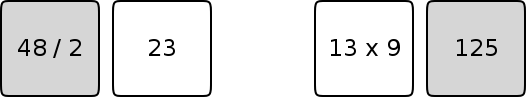
\includegraphics[width=0.5\textwidth]{./images/quantitative-reasoning.png}
    \caption[Juego de razonamiento cuantitativo]{Decisiones de ejemplo para juegos de razonamiento cuantitativo: ¿Qué cuadrado de cada pareja tiene un valor mayor?}
  \end{center}  
\end{figure}

\end{itemize}

\subsection{Atención}

Este subconjunto de habilidades mentales se subdivide en 2 aspectos: Concentración y Campo visual.

\begin{itemize}

\item {\bf Concentración}

La concentración es la habilidad mental consistente en fijar los sentidos y pensamientos en una única tarea, objeto, etc. discriminando al resto. Es el filtrado de información sensorial, atendiendo una única fuente y discriminando el resto.

Los juegos de concentración consistirán en el enfrentamiento del jugador a una situación en la que tenga que centrarse en un único elemento de un conjunto homogéneo. Un posible juego de este tipo puede ser aquel que muestre una serie de objetos iguales apuntando en diferentes direcciones, obligando al jugador a indicar la dirección en la que apunta uno sólo de ellos. Cada grupo debe ser diferente, pero el objetivo debe seguir un patrón sencillo para que el usuario lo localice rápido y pueda indicar su respuesta. La figura \ref{fig::game-focus} muestra una posible aproximación, en la que los elementos son flechas y el jugador debe indicar dónde apunta la del medio.

\begin{figure}[h]
  \begin{center}
    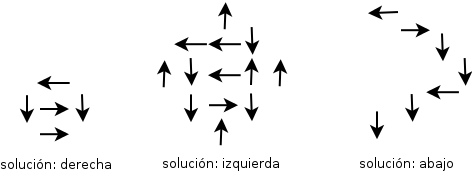
\includegraphics[width=0.8\textwidth]{./images/game-focus.png}
    \caption[Juego de concentración]{Situación de ejemplo para un juego de concentración. El jugador indica (por ejemplo mediante las teclas de dirección), la dirección en la que el elemento central apunta.}
    \label{fig::game-focus}
  \end{center}  
\end{figure}

\item {\bf Campo visual}

El campo visual es el espacio que un individuo puede ver en un instante sin mover sus ojos. El diseño de juegos destinados a la estimulación de esta habilidad es sencillo: basta con mostrar varios elementos repartidos por el espacio de juego de forma simultánea y luego, tras ocultarlos, solicitar al jugador que realice algún tipo de tarea con los objetos que se mostraron y ya no aparecen. Por ejemplo, se pueden mostrar varios números y, después de ocultarlos, pedirle al usuario que haga click en las ubicaciones aproximadas de los números por orden creciente o decreciente de valor.

\end{itemize}

\subsection{Velocidad de procesamiento}

Grupo mental centrado en la minimización del tiempo de respuesta ante estímulos y situaciones problemáticas. Se divide en las siguientes habilidades: Procesamiento de información y Orientación espacial:

\begin{itemize}

\item {\bf Procesamiento de información}

Habilidad consistente en la interpretación de la información sensorial. Tiene una relación directa con la capacidad de adaptación a los cambios del entorno.

Los juegos dedicados al entrenamiento del procesamiento de información consistirán en una serie de elementos mostrados secuencialmente, de uno en uno, de tal forma que algunos se repitan de forma consecutiva. Cuando el jugador ve cada elemento, indica si éste es exactamente igual que el anterior mostrado o no. Al responder se pasa al siguiente objeto y así sucesivamente. El objetivo es responder de forma correcta el mayor número de veces en un tiempo limitado.

\item {\bf Orientación espacial}

La orientación espacial consiste en la consciencia tridimensional de la situación de un individuo en un entorno físico.

Los juegos dedicados a entrenar esta habilidad consistirán en un espacio bidimensional sobre el que se situarán elementos cuya posición memorizar. Después el mapa sufrirá algún tipo de transformación de {\it efecto espejo} o rotación y el jugador tendrá que localizar dichas posiciones sobre el mapa modificado. Alternativamente, para el caso concreto de los juegos multijugador, otra posibilidad sería la de resolver un laberinto simétrico, empezando cada jugador por un extremo y compitiendo por llegar antes que el otro al centro del laberinto. Dicho laberinto deberá sufrir transformaciones como las mencionadas, de tal manera que el desplazamiento por el mismo suponga la inversión de direcciones ---si el laberinto es rotado 90 grados en sentido horario, en el nuevo laberinto resultante las direcciones se verían alteradas: para desplazarse hacia arriba habría que usar la tecla izquierda, para moverse hacia la derecha habría que utilizar la tecla de dirección hacia arriba, y así sucesivamente---.

La figura \ref{fig::spatial-orientation} muestra un ejemplo de laberinto multijugador para un juego de estimulación de la orientación espacial.

\begin{figure}[h]
  \begin{center}
    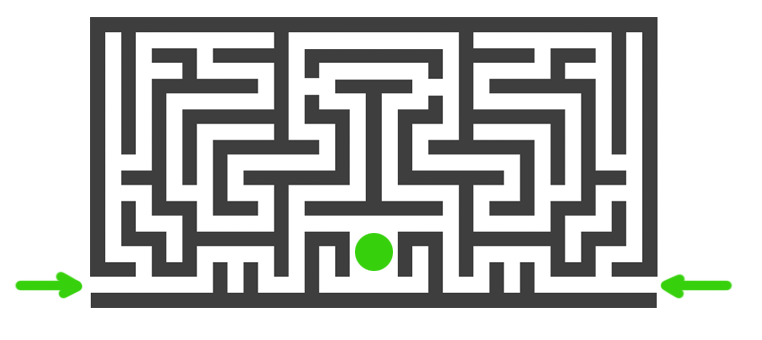
\includegraphics[width=0.8\textwidth]{./images/game-spatial-orientation.png}
    \caption{Escenario de ejemplo para un juego multijugador de orientación espacial}
    \label{fig::spatial-orientation}
  \end{center}  
\end{figure}


\end{itemize}

\subsection{Flexibilidad}

La flexibilidad es el subconjunto más amplio de habilidades mentales: {\it control de impulsos}, {\it planificación}, {\it conmutación de tareas} y {\it fluidez verbal} constituyen los aspectos relacionados con esta capacidad:

\begin{itemize}

\item {\bf Control de impulsos}

Como principal aspecto diferenciador entre el ser humano y el resto de animales, el control de impulsos permite priorizar unos objetivos por encima de posibles impulsos naturales.

Existen algunos juegos típicos relacionados con el control de impulsos que son muy buenos candidatos para ser implementados para BreakBrain. Son los juegos en los que se muestran palabras que representan a un color escritas en color (el mismo u otro). Por ejemplo se puede repetir de forma aleatoria, alternando los colores en los que las palabras aparecen escritas. El jugador debe indicar cuándo coincide el nombre del color representado por la palabra y el color en el que aparece.

\begin{figure}[h]
  \begin{center}
    
\includegraphics[width=0.6\textwidth]{./images/game-impulse.png}
    \caption{Ejemplo de prueba para ejercitar el control de impulsos}
  \end{center}  
\end{figure}

\item {\bf Planificación}

La planificación es la ordenación de tareas por prioridad a lo largo de un periodo temporal. Los juegos destinados a entrenar esta habilidad deben centrarse en la preparación de rutas sobre un escenario mediante pequeños cambios que vayan construyendo el camino. Esos cambios deben estar limitados en número o, alternativamente, utilizar los movimientos como penalización temporal para calcular la puntuación.

\item {\bf Conmutación de tareas}

La conmutación de tareas es la adaptación de la atención intercambiando entre diferentes ejercicios. Dependiendo de la situación (tarea actual) será conveniente actuar de una forma y no de otra.

Los juegos destinados a estimular y entrenar la habilidad de conmutación de tareas deben definir situaciones diferentes y asociar a cada una de ellas una forma de proceder. Una vez expuestas al jugador, dichas situaciones se alternarán de forma continuada y el jugador tendrá que proceder como se espera en cada una de ellas. La figura \ref{fig::game-switch} muestra un ejemplo sencillo en el que varias flechas se desplazan en la misma dirección (diferente en cada actividad puntuable). Existen dos situaciones:

\begin{itemize}
\item Las flechas son rojas: el jugador debe indicar en qué dirección se mueven
\item Las flechas son verdes: el jugador debe indicar a qué dirección apuntan
\end{itemize}

Los dos escenarios se repiten, alternándose de forma aleatoria. El jugador debe responder, indicando la dirección que corresponda según la situación, en el menor tiempo posible.

\begin{figure}[h]
  \begin{center}
    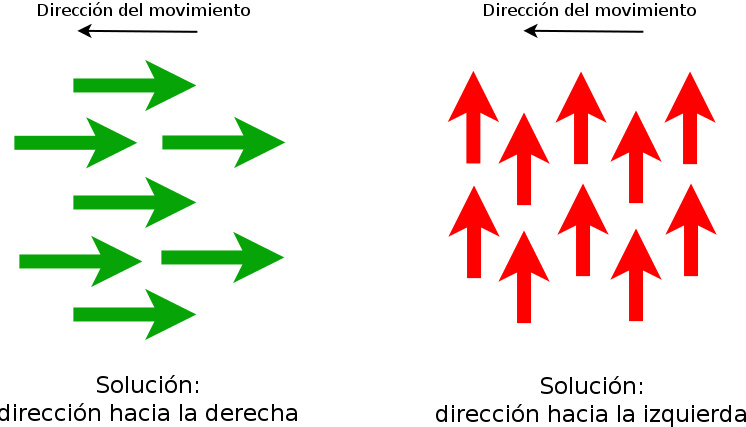
\includegraphics[width=0.6\textwidth]{./images/game-switch.png}
    \caption{Ejemplo de prueba para entrenar la conmutación de tareas}
    \label{fig::game-switch}
  \end{center}  
\end{figure}

\item {\bf Fluidez verbal}

Esta habilidad consiste en el acceso rápido al vocabulario conocido durante una tarea de escritura o una conversación. Resulta de vital importancia en la comunicación.

Los juegos dedicados a entrenar la fluidez verbal deben ofrecer partes de palabras (por ejemplo las dos o tres primeras letras) y permitir que el jugador vaya introduciendo palabras que cumplan ese patrón. Cada palabra correcta sumará una puntuación directamente proporcional a la longitud de la misma.

\end{itemize}


\begin{figure}[H]
  \begin{center}
    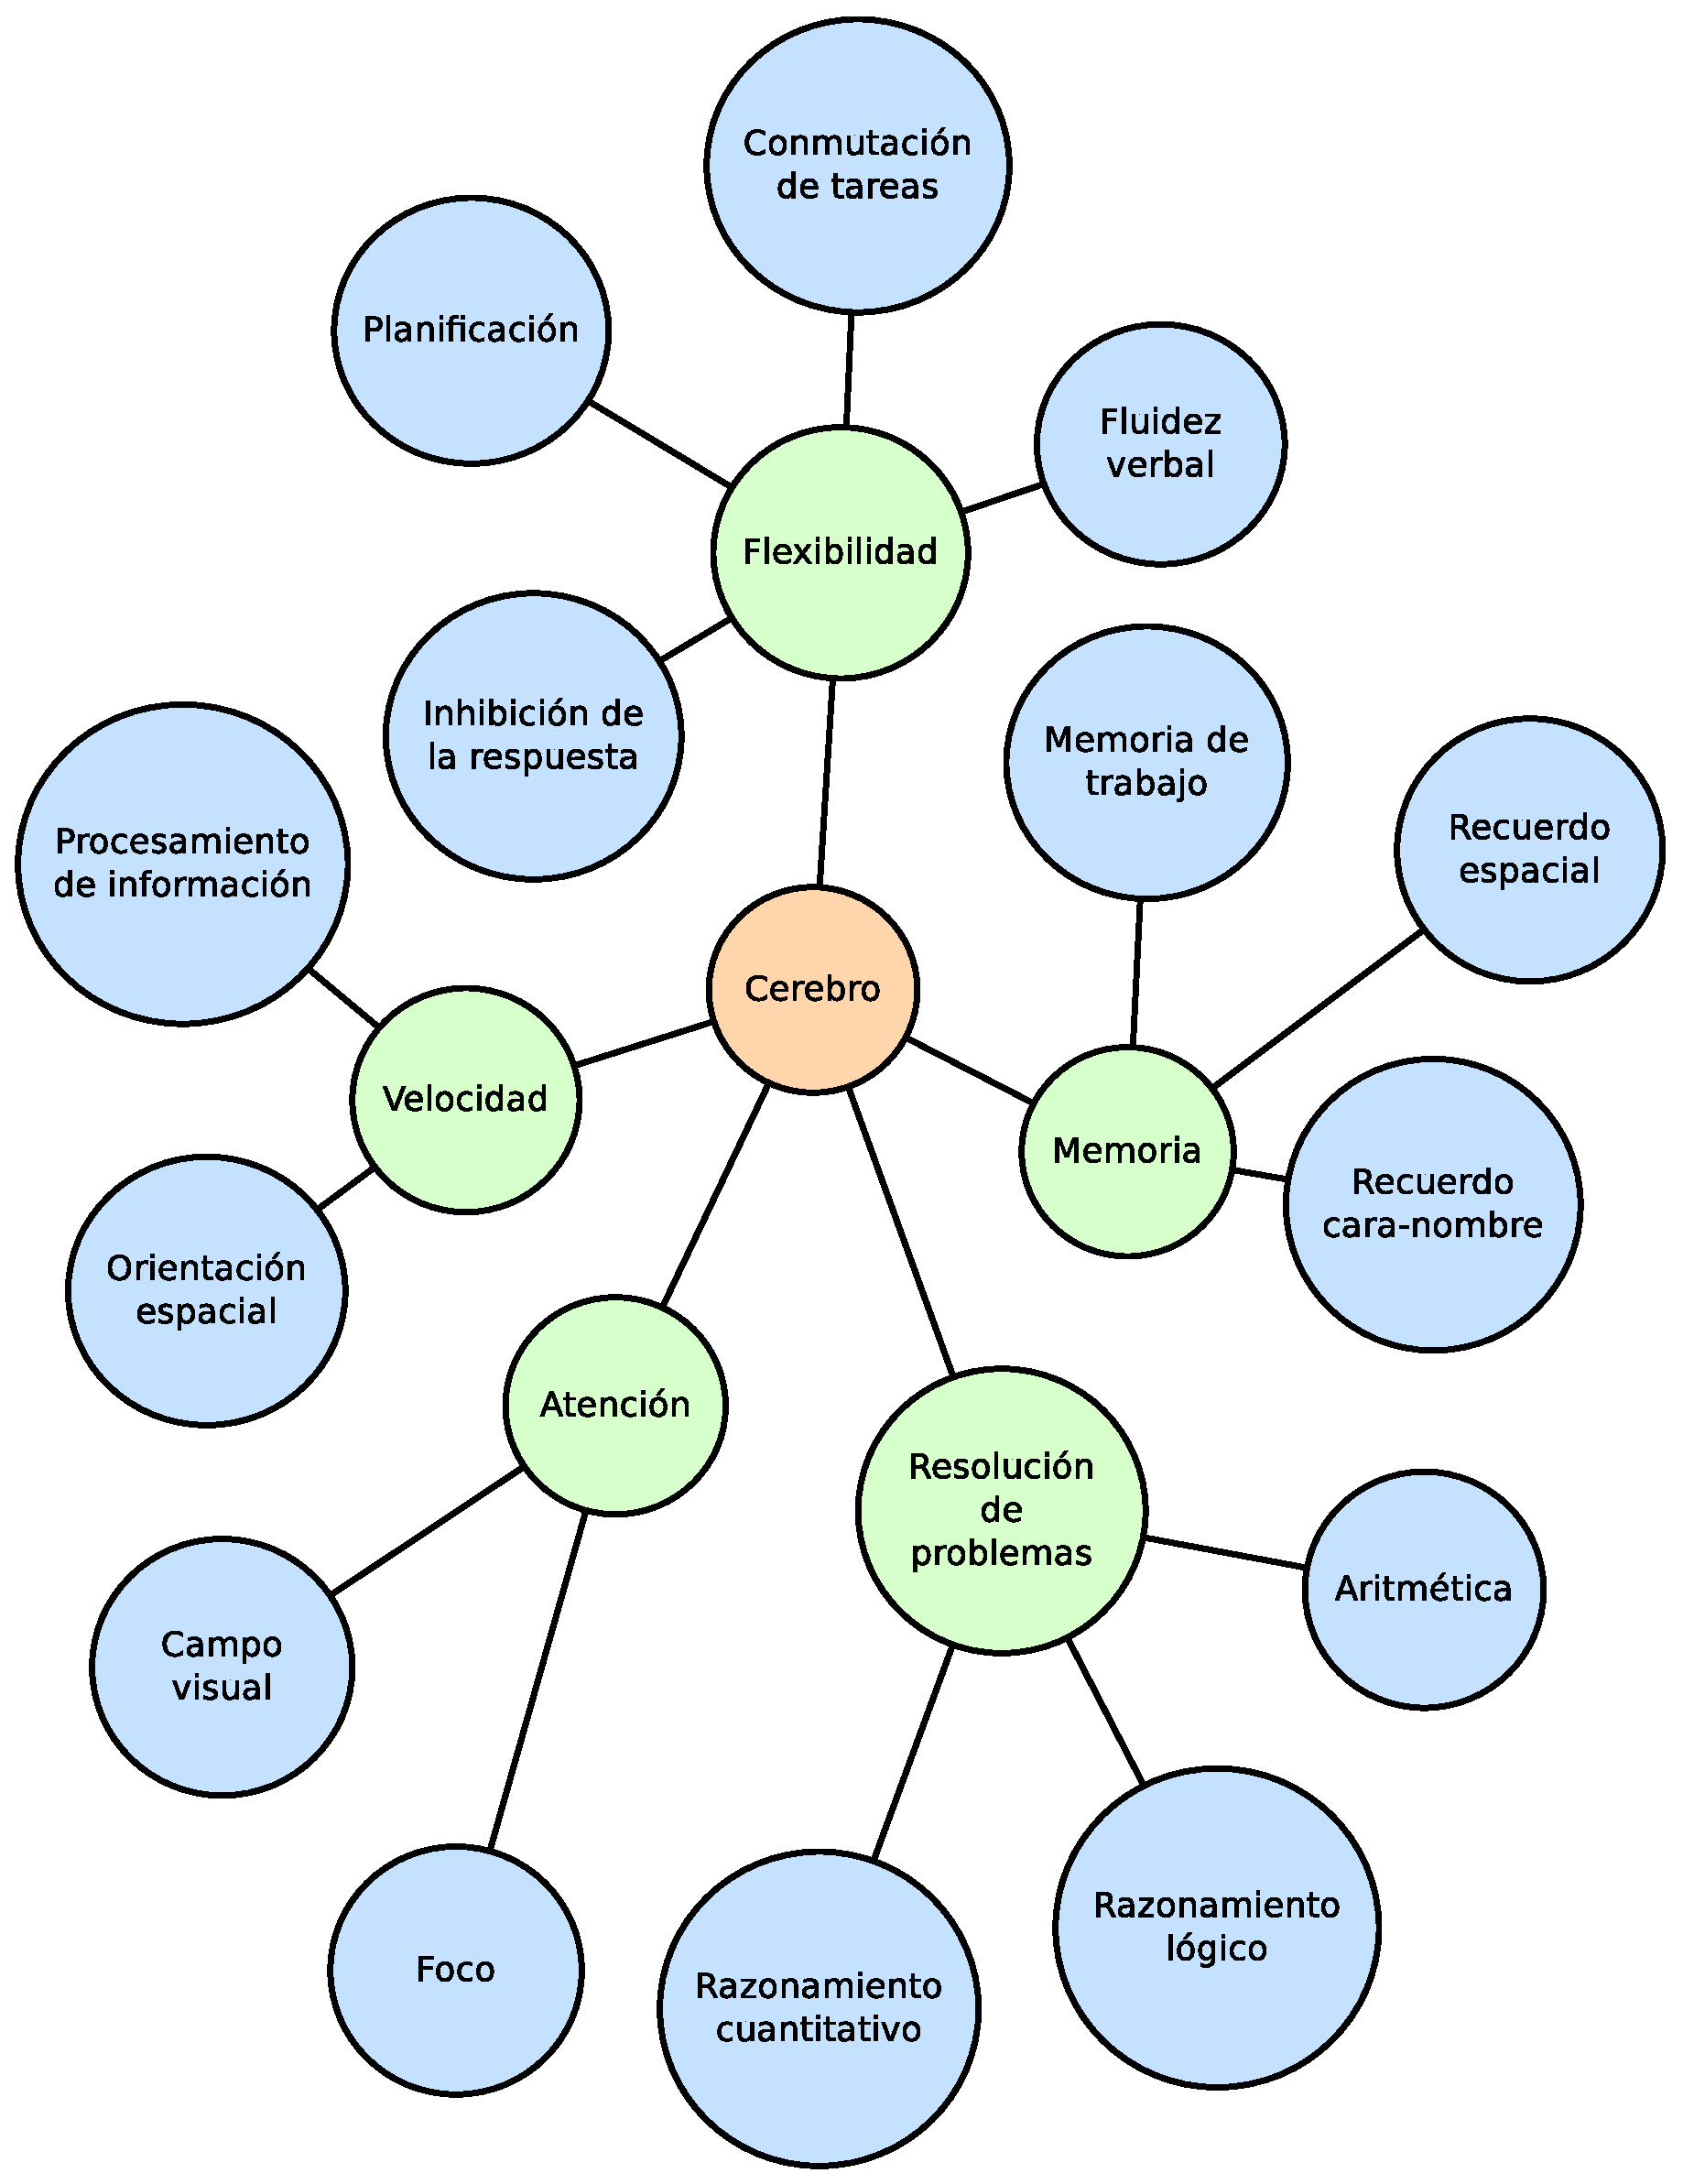
\includegraphics[scale=0.48]{images/games-diagram-esp.eps}
    \caption{Diagrama de capacidades y habilidades mentales}
    \label{fig::habilidades}
  \end{center}
\end{figure}


\section{Medición cuantitativa de la evolución cerebral}

A lo largo de esta sección se expondrán los conceptos básicos del diseño de la plataforma, para después desarrollar el sistema de puntuación de partidas y el conjunto de variables cerebrales que posibilitarán, por un lado la medición de la evolución de entrenamiento, y por otro la clasificación y recomendación de usuarios y juegos.

\subsection{Juegos, partidas y actividades puntuables}
\label{sec::juegos-partidas-actividades}

El diseño de BreakBrain hace distinción entre tres conceptos principales: juegos, actividades puntuables y partidas. En la figura \ref{fig::juegos-partidas-actividades} se ofrece una visión gráfica de la relación entre estos términos.

Resulta de vital importancia comprender bien estos conceptos para poder comprender el sistema de medición de la evolución de entrenamiento que ha sido creado en torno a ellos.

\subsubsection{Juego}

Un juego es una pequeña aplicación interactiva, centrada en una única habilidad mental (perteneciente a una capacidad), integrada en la plataforma y que permite su utilización por parte de uno o más usuarios de forma simultánea.

En base a la cantidad de jugadores que puedan enfrentarse entre sí en un juego, distinguimos entre juegos monojugador y juegos multijugador:

\begin{itemize}
\item {\bf Juegos monojugador}

Se trata de juegos diseñados para ser utilizados por un único usuario. No supone ningún tipo de interacción con otros usuarios. En este tipo de juegos no se gana o se pierde, sino que el resultado de los mismos es un valor cuantitativo que indica el grado de éxito de la partida (término que se estudia más adelante).

\item {\bf Juego multijugador}

En este caso se trata de juegos diseñados para ser utilizados por dos jugadores a la vez, suponiendo un enfrentamiento entre ellos. Sólo un jugador de los dos puede ganar cada ronda o partida (término que se estudia más adelante).

\end{itemize}

\subsubsection{Partida}

Una partida es cada una de las instancias jugables de un juego. Para ser más claros, cuando dos jugadores se encuentran jugando al mismo juego individual, cada uno en su máquina y sin realizar interacción alguna con el otro, cada uno de esos jugadores está jugando realmente una partida distinta del mismo juego.

Por otro lado, cuando dos jugadores se enfrentan cara a cara a un juego, compitiendo el uno contra el otro, ambos se encuentran en una misma partida de dicho juego. Obviamente en este caso siempre se tratará de juegos multijugador.

\subsubsection{Actividad puntuable}

La actividad puntuable es la unidad mínima jugable y, por lo tanto, la unidad mínima de entrenamiento y puntuación. Cada partida está compuesta por varias actividades puntuables. Por ejemplo, dado un juego de memoria en el que el usuario tiene que recordar la localización de grupos de objetos, cada actividad puntuable sería cada distribución de objetos a la que el usuario debe enfrentarse y resolver.

En base al número de actividades puntuables que las compongan, distinguimos entre los siguientes tipos de partidas:

\begin{itemize}
\item {\bf Partidas de corta duración}: Partida formada por 10 actividades puntuables
\item {\bf Partidas de duración media}: Partida formada por 30 actividades puntuables
\item {\bf Partidas de larga duración}: Partida formada por 50 actividades puntuables
\end{itemize}

\begin{figure}[H]
  \begin{center}
    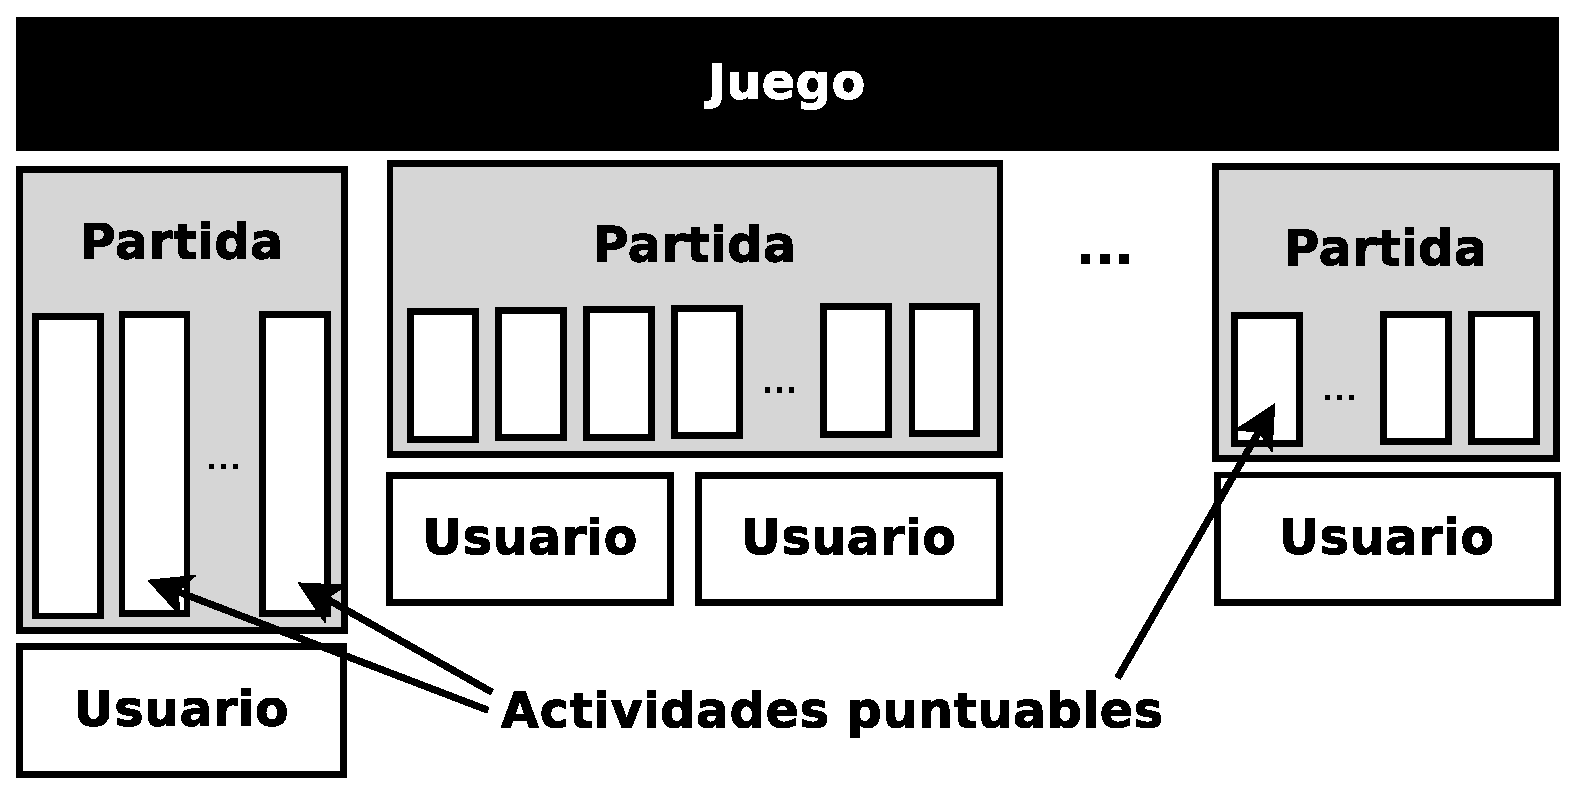
\includegraphics[width=0.8\textwidth]{images/juegos-partidas-actividades.eps}
    \caption{Juegos, partidas y actividades puntuables}
    \label{fig::juegos-partidas-actividades}
  \end{center}
\end{figure}

\subsection{Puntuación de partidas}

Tal y como se ha explicado en la sección \ref{sec::juegos-partidas-actividades}, una partida $p$ está compuesta por varias actividades puntuables $a_i$. La puntuación de una partida, $s_{p}$, es la suma de las puntuaciones obtenidas en cada actividad puntuable:


\begin{equation}
s_{p} = \sum\limits_{i = 0}^A s_i
\label{eq:partida}
\end{equation}

siendo $A$ el número total de actividades puntuables completadas en la partida $p$, y $s_i$ la puntuación de cada una de esas actividades.

La puntuación de cada actividad, $s_i$, se basa en dos aspectos: el tiempo empleado para completarla, $t_i$, y la valoración de éxito de la misma, $e_i$. Esta valoración de éxito puede ser satisfactoria o no satisfactoria, lo que matemáticamente se traduce en un 1 o un 0. Por otro lado, el tiempo $t_i$ debe encontrarse normalizado entre 0 y 1, para lo cual basta con dividir el tiempo empleado en realizar la actividad $i$ entre el tiempo empleado en realizar la actividad que más duración haya tenido. Teniendo en cuenta ambos aspectos, la puntuación de una actividad puntuable $a_i$ es la siguiente:

\begin{equation}
s_i = \frac{1}{t_i} \cdot e_i
\end{equation}

Reemplazando esta expresión en la ecuación \ref{eq:partida}, tenemos:

\begin{equation}
s_{p} = \sum\limits_{i = 0}^A \frac{1}{t_i} \cdot e_i
\end{equation}

Las actividades puntuables que no hayan sido completadas reciben una puntuación $s_i = 0$. Dependiendo del tipo de partida, será o no posible darla por finalizada sin haber completado todas las actividades puntuables que la constituyen:

\begin{itemize}
\item {\bf Puntuación en partidas monojugador}: el jugador recibe los puntos obtenidos en todas las actividades puntuables que constituyen la partida al finalizar la misma.
\item {\bf Puntuación en partidas multijugador}: una vez finalizadas todas las actividades puntuables de la partida por parte de uno de los jugadores, éste es considerado vencedor y la partida termina. Ambos jugadores reciben los puntos obtenidos durante la misma. En el caso del jugador perdedor, recibirá la puntuación de las actividades puntuables que haya completado satisfactoriamente antes de que el otro jugador haya terminado.
\end{itemize}

Teniendo en cuenta todo lo anterior, una partida $p$ formada por $A$ actividades puntuables tendrá una puntuación $s_p$ tal que $0 \leq s_p \leq A$.

\subsection{Variables de clasificación}
\label{sec::variables-perfil-usuario}

El perfil de cada usuario contiene la puntuación de cada habilidad cerebral, calculada mediante la suma de las puntuaciones obtenidas en cada partida de cada juego destinado a estimular esa habilidad. Además de ello contiene otras variables, como la cantidad de partidas ganadas, el sexo del individuo, etc. Todas estas variables se clasifican en 3 grupos:

\subsubsection{Variables estáticas o de agrupación}

\begin{itemize}
\item {\tt sex}: Sexo (hombre o mujer)
\item {\tt age}: Edad
\item {\tt keywords}: Palabras clave
\item {\tt training-interests}: Lista de habilidades mentales que el usuario está interesado en entrenar
\end{itemize}

\subsubsection{Variables dinámicas mentales}

\begin{itemize}
\item {\tt memory}: puntuación en el área de Memoria. Se trata de la suma normalizada de las siguientes tres puntuaciones:
  \begin{itemize}
  \item {\tt working-memory}: puntuación en memoria de trabajo.
  \item {\tt spatial-memory}: puntuación en memoria espacial
  \item {\tt face-name}: puntuación en memoria de asociación nombre-cara
  \end{itemize}
\item {\tt problem-solving}: puntuación en el área de Resolución de problemas. Se calcula mediante la suma normalizada de las siguientes tres puntuaciones:
  \begin{itemize}
  \item {\tt arithmetic}: puntuación en aritmética.
  \item {\tt logical-reasoning}: puntuación en razonamiento lógico.
  \item {\tt quantitative-reasoning}: puntuación en razonamiento cuantitativo.
  \end{itemize}
\item {\tt attention}: puntuación en la capacidad de Atención. Su valor es la suma normalizada de los valores de las siguientes dos variables:
  \begin{itemize}
  \item {\tt focus}: puntuación en la habilidad de concentración
  \item {\tt visual-field}: puntuación en campo visual
  \end{itemize}
\item {\tt speed}: puntuación en el área de Velocidad de procesamiento. Se trata de la suma normalizada de las siguientes dos variables:
  \begin{itemize}
  \item {\tt information-processing}: puntuación en procesamiento de la información
  \item {\tt spatial-orientation}: puntuación en orientación espacial
  \end{itemize}
\item {\tt flexibility}: puntuación en la capacidad de Flexibilidad. Se computa mediante la suma normalizada de las siguientes cuatro variables:
  \begin{itemize}
  \item {\tt response-inhibition}: puntuación en control de impulsos
  \item {\tt planning}: puntuación en planificación
  \item {\tt task-switching}: puntuación en conmutación de tareas
  \item {\tt verbal-fluency}: puntuación en fluidez verbal
  \end{itemize}
\end{itemize}

\subsubsection{Variables dinámicas sociales}

\begin{itemize}
\item {\tt followers}: cantidad de personas que siguen al usuario.
\item {\tt followees}: cantidad de personas a las que el usuario sigue.
\end{itemize}


\begin{table}[H]
\begin{footnotesize}
\begin{center}  
\begin{sideways}
\begin{tabular}{|c|l|l|l|}
\hline
\tabheadformat
\tabhead{Grupo} & \tabhead{Habilidad} & \tabhead{Descripción} & \tabhead{Entrenamiento mediante juegos} \\
\hline\hline
\multirow{6}{*}{\begin{sideways}Memoria\end{sideways}} & Memoria  & Almacenamiento temporal de información & Mostrar pequeñas cantidades de información para memorizar \\
 & de trabajo & durante el desarrollo de una tarea. & y después requerirlas de algún modo. \\
\cline{2-4}
 & Memoria & Información del entorno, localización de objetos & Ofrecer un paisaje de objetos para su memorización \\
 & espacial & y orientación en el espacio. & y solicitar la reconstrucción del mismo.\\
\cline{2-4}
 & Memoria & Relación entre objetos y etiquetas asociadas & Mostrar la relación existente entre varios objetos y etiquetas.\\
 & nombre-cara & a dichos objetos.& El jugador deberá memorizar esas relaciones y reconstruirlas.\\
\hline\hline

\multirow{6}{*}{\begin{sideways}Res. prob.\end{sideways}} & Aritmética & Realización de operaciones matemáticas sencillas & Enfrentar al jugador a gran cantidad de operaciones sencillas.\\
\cline{2-4}
 & Razonamiento & Inducción de reglas lógicas & Mostrar elementos que cumplen o no una regla lógica para \\
 & lógico & a partir de casos concretos. & que el jugador la adivine y la aplique a otros elementos. \\
\cline{2-4}
 & Razonamiento & Realización de estimaciones y toma de decisiones & Ofrecer grupos de elementos cuantificables para que \\
 & cuantitativo & en base a ellas. & el jugador elija rápidamente el de mayor o menor valor. \\
\hline\hline

\multirow{4}{*}{\begin{sideways}Atención\end{sideways}} & Concentración & Fijación y dedicación de las actividades sensoriales & Ofrecer grupos de elementos en los que el jugador tenga que \\
 &  & a una única tarea. & prestar atención a alguna propiedad de uno sólo de ellos. \\
\cline{2-4}
 & Campo & Espacio tridimensional visible por un individuo sin & Mostrar y ocultar elementos en el espacio de juego. El jugador deberá \\
 & visual & realizar movimientos oculares. & realizar alguna tarea con las ubicaciones donde aparecían y su valor. \\
\hline\hline

\multirow{4}{*}{\begin{sideways}Velocidad\end{sideways}} & Procesamiento & Interpretación de la información sensorial. &  Ofrecer una secuencia de elementos, algunos idénticos consecutivamente. \\
 & de Información & Adaptación al cambio. & El jugador debe decir si cada uno es igual al anterior o no. \\
\cline{2-4}
 & Orientación & Consciencia tridimensional de la situación & Mostrar elementos distribuidos en un espacio. Tras una transformación \\
 & espacial & de uno mismo en el espacio. & del mismo, el jugador deberá localizar dichas posiciones. \\
\hline\hline
\multirow{8}{*}{\begin{sideways}Flexibilidad\end{sideways}} & Control de & Priorización de objetivos personales por & Jugar con los colores y su representación textual. El jugador \\
 & impulsos & encima de los impulsos animales. & deberá poder prestar atención a un sólo aspecto: el color o el texto. \\
\cline{2-4}
& Planificación & Priorización alterna de unas tareas sobre otras & Ofrecer un espacio bidimensional maleable mediante cambios. El jugador \\
& & en un periodo temporal. & construirá un camino usando el efecto de esos cambios. \\
\cline{2-4}
& Conmutación & Intercambio de la atención entre ejercicios de forma & Ofrecer situaciones diferentes, cada una con una misión. \\
& de tareas & arbitraria e intermitente. & Las situaciones van cambiando, y en cada una el jugador debe proceder. \\
\cline{2-4}
& Fluidez  & Recuperación rápida del vocabulario durante & Ofrecer las primeras o últimas letras de una palabra. El jugador \\
& verbal & una conversación fluida. & deberá enumerar palabras que cumplen ese patrón. \\
\hline
\end{tabular}
\end{sideways}
\end{center}
\end{footnotesize}
\caption{Ficha de entrenamiento de capacidades mentales}
\label{table:capacidades}
\end{table}


% <<<<<<<<<<<<<<<<<<<<<<<<<<<<<<

\section{Sistema de recomendación}

BreakBrain cuenta con un sistema de recomendación integrado que ha sido desarrollado para encontrar los usuarios y juegos más adecuados para cada usuario en cada instante. Los usuarios son recomendados para el seguimiento (suscripción a novedades y enfrentamiento en juegos), mientras que los juegos son recomendados para el entrenamiento que más se adecúe a cada instante, dependiendo de los intereses y evolución del usuario.

Para la construcción de este sistema de recomendación se ha seguido un enfoque híbrido (ver sección \ref{sec::sistemas-recomendacion}), sacando partido a las mejores características de los métodos ``basado en contenido'', ``colaborativo'', ``demográfico'', ``basado en conocimiento'' y ``basado en utilidad''.

Las variables que constituyen toda la información disponible sobre cada juego son las siguientes:

\begin{itemize}
\item {\tt capacity}: capacidad cerebral que el juego estimula (cadena de texto, enumerada).
\item {\tt hability}: habilidad cerebral (dentro de la capacidad especificada) que el juego estimula (cadena de texto, enumerada).
\item {\tt dedication}: partidas jugadas al juego por parte de cada usuario de la red social. Para BreakBrain, estos valores suponen la puntuación que el usuario asigna a cada juego, de forma que cada valoración $s_u$ que requiere el sistema de recomendación (ver sección \ref{sec::sistemas-recomendacion}) no tiene que realizarse mediante una acción explícita. Se trata de un número entero.
\end{itemize}

Por otro lado, las variables que constituyen la información de perfil y evolución del entrenamiento de los usuarios, basadas en la sección \ref{sec::variables-perfil-usuario} son las siguientes:

\begin{itemize}
\item {\tt sex}: sexo (cadena de texto, enumerada)
\item {\tt age}: edad (número entero)
\item {\tt keywords}: palabras clave (vector de cadenas de texto)
\item {\tt training-interests}: habilidades mentales en las que el usuario está interesado. (vector de cadenas de texto)
\item {\tt memory}: puntuación en el área de Memoria. Suma normalizada de:
  \begin{itemize}
  \item {\tt working-memory}: puntuación en memoria de trabajo (número entero).
  \item {\tt spatial-memory}: puntuación en memoria espacial (número entero).
  \item {\tt face-name}: puntuación en memoria de asociación nombre-cara (número entero).
  \end{itemize}
\item {\tt problem-solving}: puntuación en el área de Resolución de problemas. Suma normalizada:
  \begin{itemize}
  \item {\tt arithmetic}: puntuación en aritmética (número entero).
  \item {\tt logical-reasoning}: puntuación en razonamiento lógico (número entero).
  \item {\tt quantitative-reasoning}: puntuación en razonamiento cuantitativo (número entero).
  \end{itemize}
\item {\tt attention}: puntuación en la capacidad de Atención. Suma normalizada:
  \begin{itemize}
  \item {\tt focus}: puntuación en la habilidad de concentración (número entero).
  \item {\tt visual-field}: puntuación en campo visual (número entero).
  \end{itemize}
\item {\tt speed}: puntuación en el área de Velocidad de procesamiento. Suma normalizada de:
  \begin{itemize}
  \item {\tt information-processing}: puntuación en procesamiento de la información (número entero).
  \item {\tt spatial-orientation}: puntuación en orientación espacial (número entero).
  \end{itemize}
\item {\tt flexibility}: puntuación en la capacidad de Flexibilidad. Suma normalizada de:
  \begin{itemize}
  \item {\tt response-inhibition}: puntuación en control de impulsos (número entero).
  \item {\tt planning}: puntuación en planificación (número entero).
  \item {\tt task-switching}: puntuación en conmutación de tareas (número entero).
  \item {\tt verbal-fluency}: puntuación en fluidez verbal (número entero).
  \end{itemize}
\item {\tt followers}: personas que siguen al usuario (vector de cadenas de texto, identificadores de usuario).
\item {\tt followees}: personas a las que el usuario sigue (vector de cadenas de texto, identificadores de usuario).
\end{itemize}

La tabla \ref{table:variables-resumen} muestra el conjunto de variables que representan toda la información de la que BreakBrain dispone sobre los usuarios y los juegos.


\begin{table}
  \begin{center}
    \begin{tabular}{lcc}
      \hline
      \tabheadformat
      {\bf Variable} & {\bf Tipo} & {\bf Valores} \\
      \hline
      {\tt capacity} & Enumeración & memory, problem-solving... \\
      {\tt hability} & Enumeración & working-memory, spatial-memory... \\
      {\tt dedication} & Número entero & $\geq 0$ \\
      \hline
      \tabheadformat
      {\bf Variable} & {\bf Tipo} & {\bf Valores} \\
      \hline
      {\tt sex} & Enumeración & hombre, mujer \\
      {\tt age} & Número entero & $\geq 0$ \\
      {\tt keywords} & Vector de cadenas & [``key1'', ``key2'', ...] \\
      {\tt training-interests} & Vector de enumeración & [``focus'', ``visual-field'', ...] \\
      {\tt memory} & Número decimal & $[0-1]$ \\
      {\tt working-memory} & Número entero & $\geq 0$ \\
      {\tt spatial-memory} & Número entero & $\geq 0$ \\
      {\tt face-name} & Número entero & $\geq 0$ \\
      {\tt problem-solving} & Número decimal & $[0-1]$ \\
      {\tt arithmetic} & Número entero & $\geq 0$ \\
      {\tt logical-reasoning} & Número entero & $\geq 0$ \\
      {\tt quantitative-reasoning} & Número entero & $\geq 0$ \\
      {\tt attention} & Número decimal & $[0-1]$ \\
      {\tt focus} & Número entero & $\geq 0$ \\
      {\tt visual-field} & Número entero & $\geq 0$ \\
      {\tt speed} & Número decimal & $[0-1]$ \\
      {\tt information-processing} & Número entero & $\geq 0$ \\
      {\tt spatial-orientation} & Número entero & $\geq 0$ \\
      {\tt flexibility} & Número decimal & $[0-1]$ \\
      {\tt response-inhibition} & Número entero & $\geq 0$ \\
      {\tt planning} & Número entero & $\geq 0$ \\
      {\tt task-switching} & Número entero & $\geq 0$ \\
      {\tt verbal-fluency} & Número entero & $\geq 0$ \\
      {\tt followers} & Número entero & $\geq 0$ \\
      {\tt followees} & Número entero & $\geq 0$ \\
      \hline
    \end{tabular}
  \end{center}
  \caption{Variables de BreakBrain sobre usuarios y juegos}
  \label{table:variables-resumen}
\end{table}

Haciendo uso de toda la información disponible se han desarrollado dos subsistemas de recomendación: uno para usuarios y otro para juegos. A continuación se expondrán los algoritmos diseñados para ambos.

\subsection{Algoritmo de recomendación de usuarios}

Para la realización de sugerencias de usuarios a los que seguir en BreakBrain se ha desarrollado un algoritmo de recomendación híbrido, diseñado a partir de los métodos {\it colaborativo} y {\it basado en contenido} (ver sección \ref{sec::tipos-sistemas-recomendacion}). Para recomendar usuarios a un usuario dado (al que llamaremos ``objetivo''), por tanto, el algoritmo hace uso de 2 datos:

\begin{itemize}
\item Los usuarios a los que ya sigue el objetivo
\item Los usuarios a los que siguen aquellos con cierta similitud al objetivo
\end{itemize}

\subsubsection{Similitud entre usuarios}

En base a lo anterior, el primer paso que debe seguir el algoritmo es encontrar los usuarios similares al objetivo. La función encargada de hacerlo tiene en cuenta las siguientes características de los usuarios:

\begin{itemize}
\item Keywords de descripción
\item Intereses de entrenamiento
\item Puntuación de capacidades mentales
\end{itemize}

En el listado \ref{pseudocodigo:similitud} se ofrece el pseudocódigo de la función encargada de encontrar usuarios similares al usuario objetivo.

\begin{listing}[caption=Función que encuentra usuarios similares al objetivo, label=pseudocodigo:similitud]
FUNCION similares (objetivo: USUARIO, usuarios: VECTOR DE USUARIO, n: INTEGER)
VARIABLES
    sim : FLOAT;
    u : USUARIO;
    similitudes : VECTOR DE (USUARIO, FLOAT)
INICIO
    PARA CADA u DE usuarios HACER
        sim := similitud(u, objetivo);
        push(similitudes, [u, sim]);
        similitudes := ordenar(similitudes);
        similitudes := head(similitudes, n);
        DEVOLVER similitudes
    FIN
FIN
\end{listing}

La similitud entre dos usuarios es calculada en base a las similitudes entre sus keywords, intereses y perfil cerebral. El listado \ref{codigo:similitud} muestra el código JavaScript encargado de realizar dicho cálculo.

\begin{listing}[caption=Algoritmo de recomendación de usuarios, label=codigo:similitud, language=JavaScript]
/**
 * Calcula la similitud entre 2 usuarios
 * @param {object} user1 Primer usuario
 * @param {object} user2 Segundo usuario
 * @returns {number} Similitud entre usuarios [0-1]
 */
var usersSimilarity = function (user1, user2) {

	/**
	 * Calcula la similitud entre dos vectores de keywords
	 */
	var keywordsSimilarity = function (keywords1, keywords2) {

		var maxLen = Math.max(keywords1.length, keywords2.length);
		var intersection = keywords1.filter(function (elem) {
			return keywords2.indexOf(elem) >= 0;
		});
		return intersection.length / maxLen;
	};

	/**
	 * Calcula la similitud entre dos vectores de intereses
	 */
	var interestsSimilarity = function (interests1, interests2) {

		return keywordsSimilarity(interests1, interests2);
	};

	/**
	 * Calcula la similitud entre las capacidades mentales de dos sujetos
	 */
	var capacitiesSimilarity = function (brain1, brain2) {

		var similarity = 0;
		var len = 0;
		for (var capacity in brain1) {
			var cap1 = brain1[capacity];
			var cap2 = brain2[capacity];
			var diff = Math.abs(cap1 - cap2);
			similarity += 1 - diff;
			len ++;
		}
		return similarity / len;
	};

	var keywordsSim = keywordsSimilarity(user1.keywords, user2.keywords);
	var interestsSim = interestsSimilarity(user1.interests, user2.interests);
	var brainSim = capacitiesSimilarity(user1.brain, user2.brain);

	return (keywordsSim + interestsSim + brainSim) / 3;
};
\end{listing}

En base a lo anterior, el algoritmo diseñado para realizar las sugerencias de seguimiento de usuarios para un objetivo dado es el mostrado, mediante pseudocódigo, en el listado \ref{pseudocodigo:recomendacion-usuarios}.

\begin{listing}[caption=Algoritmo de recomendación de usuarios, label=pseudocodigo:recomendacion-usuarios]
FUNCION recomienda usuarios (objetivo: USUARIO, usuarios: VECTOR DE USUARIO, n: INTEGER)
VARIABLES
    sim : FLOAT;
    u : USUARIO;
    similares : VECTOR DE (USUARIO, FLOAT);
    recomendacion : VECTOR DE (USUARIO, FLOAT);
    recomendacion2 : VECTOR DE (USUARIO, FLOAT);
    fwees : VECTOR DE (USUARIO);
INICIO
    PARA CADA u DE objetivo.followees HACER
        fwees := u.followees;
        PARA CADA u2 DE fwees HACER
            sim := similitud(u2, objetivo);
            push(recomendacion, [u, sim]);
            recomendacion := ordenar(recomendacion);
            recomendacion := head(recomendacion, n / 2);
        FIN
    FIN
    similares := similares(objetivo, usuarios, n);
    PARA CADA u DE similares HACER
        fwees := u.followees;
        PARA CADA u2 DE fwees HACER
            sim := similitud(u2, objetivo);
            push(recomendacion2, [u, sim]);
            recomendacion2 := ordenar(recomendacion2);
            recomendacion2 := head(recomendacion2, n / 2);
        FIN
    FIN
    recomendacion := concatena(recomendacion, recomendacion2);
    recomendacion := ordenar(recomendacion);
    recomendacion := head(recomendacion, n);
    DEVOLVER recomendacion;
FIN
\end{listing}

\subsection{Algoritmo de recomendación de juegos}

Para el caso de la recomendación de juegos para un usuario objetivo se ha diseñado un algoritmo híbrido basado en los métodos de utilidad y colaborativo (ver sección \ref{sec::tipos-sistemas-recomendacion}).

La función de utilidad se calcula en base al estado cerebral del sujeto objetivo en el instante de ejecución del algoritmo, y tiene en cuenta todo el conjunto de juegos como items susceptibles de ser recomendados. El enfoque colaborativo hace uso de la información de seguimiento de usuarios para prestar atención a los juegos preferidos por los {\tt followees} del usuario objetivo.

Por tanto, la información de la que hace uso el algoritmo es la siguiente:

\begin{itemize}
\item Conjunto de juegos (cada uno con una única capacidad y habilidad definida).
\item Perfil cerebral del usuario objetivo (estado de todas las habilidades mentales).
\item Usuarios a los que el objetivo sigue.
\item Dedicación de cada usuario a cada juego.
\end{itemize}

En líneas generales, los pasos que el algoritmo diseñado sigue son los siguientes:

\begin{enumerate}
\item Ordenar las habilidades mentales del usuario objetivo por puntuación (las peor valoradas primero).
\item Filtrar los juegos, seleccionando los que estén dedicados a las 3 habilidades peor puntuadas del individuo.
\item Obtener la dedicación de cada usuario seguido por el objetivo para cada juego del subconjunto filtrado.
\item Calcular una valoración global de la dedicación para cada juego.
\item Ordenar el subconjunto de juegos en base a la dedicación.
\item Recomendar al usuario los {\tt n} primeros juegos de la lista ordenada.
\end{enumerate}

El listado \ref{pseudocodigo:games} ofrece una descripción del algoritmo de recomendación de juegos de BreakBrain.

\begin{listing}[caption=Algoritmo de recomendación de juegos, label=pseudocodigo:games]
FUNCION recomendarJuegos (objetivo: USUARIO, todosLosJuegos: VECTOR DE JUEGO, n: INTEGER)
VARIABLES
    habilidades : VECTOR DE (STRING, FLOAT);
    juegos : VECTOR DE JUEGO;
    fwees : VECTOR DE USUARIO;
    dedicacion : INTEGER;
    j : JUEGO;
INICIO
    habilidades := objetivo.habilidades;
    habilidades := ordenar(habilidades);
    juegos := filter(todosLosJuegos, habilidades);
    fwees := objetivo.followees;
    PARA CADA j DE juegos HACER
        dedicacion := 0;
        PARA CADA u DE fwees HACER
            dedicacion := dedicacion + j.dedicacion(u);
        FIN
        dedicacion := dedicacion / length(fwees);
    FIN
    juegos := ordenar(juegos, dedicacion);
    juegos := head(juegos, n);
    DEVOLVER juegos;
FIN
\end{listing}

%% \subsection{Notas personales}

%% En \ref{sec::estructuras-primarias} se habla de la generación de patrones. Esto hay que comentarlo en los juegos.

%% En \ref{sec::corteza-cerebral} se habla de las áreas de Brodmann. Debería tenerlas en cuenta ne los juegos. La experiencia en la determinación de las representaciones corticales.

%% En \ref{sec::estructuras-subcorticales} se habla de como la experiencia afecta al cerebro

%\section{Algoritmo de búsqueda de usuarios}

\chapter{Conclusiones y propuestas}
\label{chap:conclusiones}


\appendix
\appendixtitle
\chapter{Iteraciones del PUD}
\label{chap::iteraciones}

Este anexo pretende ofrecer un análisis descriptivo de las diferentes iteraciones por las que ha pasado el presente proyecto durante su desarrollo, siguiendo para ello el \acs{PUD}, como se comentó en la sección \ref{sec::pud}.

A continuación se hará un recorrido por cada iteración, explicando en qué han consistido y detallando la repercusión global de cada una. Las iteraciones están agrupadas en tres fases: Inicio, Elaboración y Construcción.

Cada iteración es detallada desde 2 puntos de vista:

\begin{itemize}
\item {\bf Local}

Con este enfoque se ofrece una descripción de en qué ha consistido la iteración. Además se detalla la proporción del desarrollo general que ha supuesto. Es importante comprender que las cifras de cada iteración no representan la repartición del esfuerzo de esa tarea, sino el porcentaje de cada artefacto que ha sido completado en esa iteración.

\item {\bf Global}

Con este enfoque se muestran los porcentajes completado y restante del desarrollo global, desde el inicio de la primera iteración hasta la finalización de la iteración en cuestión.

\end{itemize}

Al finalizar este anexo se ofrecerá una descripción gráfica de la evolución seguida durante el proceso.

\section{Iteraciones de inicio}

%% ==================================================

\subsection*{Iteración I1}

\begin{itemize}    
\item {\bf Descripción}:

Esta primera iteración se ha basado en la elaboración del análisis de un conjunto inicial de requisitos ---los más importantes--- así como el estudio de casos de uso de una parte de los mismos.

Al mismo tiempo que parte de los requisitos quedaban especificados por completo, una pequeña parte del diseño del software a construir quedaba definido.

Los artefactos que se han visto involucrados en esta iteración son, por lo tanto, el análisis de requisitos, en análisis de casos de uso y el diseño.

Esta iteración ha tenido una duración de 75 horas aproximadamente.
\end{itemize}

\begin{minipage}[c]{0.45\linewidth}
  \begin{itemize}    
  \item {\bf Desarrollo local}:
    \begin{itemize}
    \item Requisitos: 53.6\%.
    \item Casos de uso: 27.8\%.
    \item Diseño: 10\%.
    \item Implementación: 0\%.
    \item Pruebas: 0\%.
    \end{itemize}
  \item {\bf Desarrollo global}: 18.28\%
  \item {\bf Desarrollo restante}: 81.72\%
  \end{itemize}
\end{minipage}
\begin{minipage}[c]{0.45\linewidth}
  \begin{figure}[H]
    \begin{center}
      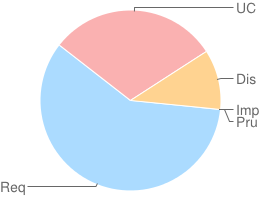
\includegraphics[width=6cm]{images/i1.png}
      % http://charts.hohli.com

      % http://chart.apis.google.com/chart?cht=p&chs=260x200&chd=s:DhPGD&chl=Imp|Req|UC|Dis|Pru&chco=abdbff,fab1b1,ffd391,ffa1fc,b6e0be&chf=bg,s,FFFFFF|c,s,FFFFFF
      \caption{Iteracción I1}
      \label{fig::i1}
    \end{center}
  \end{figure}
\end{minipage}

\section{Iteraciones de elaboración}

%% ==================================================

\subsection*{Iteración E1}

\begin{itemize}    
\item {\bf Descripción}:

Esta primera iteración de la fase de elaboración ha supuesto los primeros pasos de la implementación ---en una proporción modesta---, al tiempo que los análisis de requisitos y de casos de uso han sido ampliados.

Los artefactos que se han visto involucrados en esta iteración son, por lo tanto, el análisis de requisitos, en análisis de casos de uso, el diseño y la implementación.

Esta iteración ha tenido una duración de 50 horas aproximadamente.
\end{itemize}

\begin{minipage}[c]{0.45\linewidth}
  \begin{itemize}    
  \item {\bf Desarrollo local}:
    \begin{itemize}
    \item Requisitos: 17.8\%.
    \item Casos de uso: 22.2\%.
    \item Diseño: 15\%.
    \item Implementación: 5.2\%.
    \item Pruebas: 0\%.
    \end{itemize}
  \item {\bf Desarrollo global}: 30.3\%
  \item {\bf Desarrollo restante}: 69.7\%
  \end{itemize}
\end{minipage}
\begin{minipage}[c]{0.45\linewidth}
  \begin{figure}[H]
    \begin{center}
      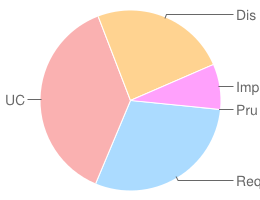
\includegraphics[width=6cm]{images/e1.png}
      % http://charts.hohli.com

      % http://chart.apis.google.com/chart?cht=p&chs=260x200&chd=s:DhPGD&chl=Imp|Req|UC|Dis|Pru&chco=abdbff,fab1b1,ffd391,ffa1fc,b6e0be&chf=bg,s,FFFFFF|c,s,FFFFFF
      \caption{Iteracción E1}
      \label{fig::e1}
    \end{center}
  \end{figure}
\end{minipage}

%% ==================================================

\subsection*{Iteración E2}

\begin{itemize}    
\item {\bf Descripción}:

Esta última etapa de la fase de Elaboración ha supuesto un pequeño avance generalizado. La mayor parte de los esfuerzos se han dedicado al diseño del software. Además se han creado las primeras pruebas unitarias.

Todos los artefactos se han visto involucrados en esta iteración: el análisis de requisitos, en análisis de casos de uso, el diseño, la implementación y las pruebas.

Esta iteración ha tenido una duración de 50 horas aproximadamente.
\end{itemize}

\begin{minipage}[c]{0.45\linewidth}
  \begin{itemize}    
  \item {\bf Desarrollo local}:
    \begin{itemize}
    \item Requisitos: 14.3\%.
    \item Casos de uso: 27.8\%.
    \item Diseño: 50\%.
    \item Implementación: 12.1\%.
    \item Pruebas: 5\%.
    \end{itemize}
  \item {\bf Desarrollo global}: 52.2\%
  \item {\bf Desarrollo restante}: 47.8\%
  \end{itemize}
\end{minipage}
\begin{minipage}[c]{0.45\linewidth}
  \begin{figure}[H]
    \begin{center}
      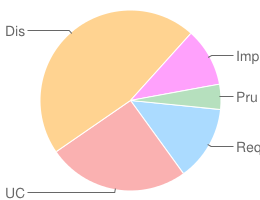
\includegraphics[width=6cm]{images/e2.png}
      % http://charts.hohli.com

      % http://chart.apis.google.com/chart?cht=p&chs=260x200&chd=s:DhPGD&chl=Imp|Req|UC|Dis|Pru&chco=abdbff,fab1b1,ffd391,ffa1fc,b6e0be&chf=bg,s,FFFFFF|c,s,FFFFFF
      \caption{Iteracción E2}
      \label{fig::e2}
    \end{center}
  \end{figure}
\end{minipage}


\section{Iteraciones de construcción}

\subsection*{Iteración C1}

\begin{itemize}    
\item {\bf Descripción}:

En esta iteración se ha realizado un pequeño esfuerzo por prácticamente terminar de definir los casos de uso. Dado que en la etapa de construcción el objetivo es centrarse en la implementación, en esta primera iteración se ha pretendido dejar prácticamente finalizados los artefactos previos a la misma.

En esta iteración están implicados todos los artefactos: análisis de requisitos, en análisis de casos de uso, diseño, implementación y pruebas.

Esta iteración ha tenido una duración de 75 horas aproximadamente.
\end{itemize}

\begin{minipage}[c]{0.45\linewidth}
  \begin{itemize}    
  \item {\bf Desarrollo local}:
    \begin{itemize}
    \item Requisitos: 3.6\%.
    \item Casos de uso: 16.6\%.
    \item Diseño: 5\%.
    \item Implementación: 2.9\%.
    \item Pruebas: 5\%.
    \end{itemize}
  \item {\bf Desarrollo global}: 58.8\%
  \item {\bf Desarrollo restante}: 41.2\%
  \end{itemize}
\end{minipage}
\begin{minipage}[c]{0.45\linewidth}
  \begin{figure}[H]
    \begin{center}
      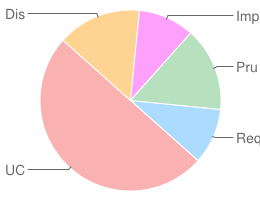
\includegraphics[width=6cm]{images/c1.png}
      % http://charts.hohli.com

      % http://chart.apis.google.com/chart?cht=p&chs=260x200&chd=s:DhPGD&chl=Imp|Req|UC|Dis|Pru&chco=abdbff,fab1b1,ffd391,ffa1fc,b6e0be&chf=bg,s,FFFFFF|c,s,FFFFFF
      \caption{Iteracción C1}
      \label{fig::c1}
    \end{center}
  \end{figure}
\end{minipage}

\subsection*{Iteración C2}

\begin{itemize}    
\item {\bf Descripción}:

Una vez el proyecto se ha centrado en la etapa de construcción, en esta iteración se realiza un gran avance en la implementación del sistema software. El análisis de requisitos queda prácticamente terminado, a excepción de algún pequeño detalle ---requisitos sencillos que surgieron a medida que el desarrollo avanzaba---, y el análisis de casos de uso se finaliza por completo.

En esta iteración están implicados todos los artefactos: análisis de requisitos, en análisis de casos de uso, diseño, implementación y pruebas, con un peso muy importante para la implementación.

Esta iteración ha tenido una duración de 125 horas aproximadamente.
\end{itemize}

\begin{minipage}[c]{0.45\linewidth}
  \begin{itemize}    
  \item {\bf Desarrollo local}:
    \begin{itemize}
    \item Requisitos: 7.1\%.
    \item Casos de uso: 5.6\%.
    \item Diseño: 5\%.
    \item Implementación: 30.6\%.
    \item Pruebas: 23.4\%.
    \end{itemize}
  \item {\bf Desarrollo global}: 73.1\%
  \item {\bf Desarrollo restante}: 26.9\%
  \end{itemize}
\end{minipage}
\begin{minipage}[c]{0.45\linewidth}
  \begin{figure}[H]
    \begin{center}
      \includegraphics[width=6cm]{images/c2.png}
      % http://charts.hohli.com

      % http://chart.apis.google.com/chart?cht=p&chs=260x200&chd=s:DhPGD&chl=Imp|Req|UC|Dis|Pru&chco=abdbff,fab1b1,ffd391,ffa1fc,b6e0be&chf=bg,s,FFFFFF|c,s,FFFFFF
      \caption{Iteracción C2}
      \label{fig::c2}
    \end{center}
  \end{figure}
\end{minipage}

\subsection*{Iteración C3}

\begin{itemize}    
\item {\bf Descripción}:

Continuando con un esfuerzo mayor para la implementación, esta iteración pretende además avanzar de forma importante con el diseño. Las pruebas son mejoradas y ampliadas.

En esta iteración están implicados los artefactos de análisis de requisitos, diseño, implementación y pruebas, con un peso muy importante, como ya se ha mencionado, para las pruebas.

Esta iteración ha tenido una duración de 80 horas aproximadamente.
\end{itemize}

\begin{minipage}[c]{0.45\linewidth}
  \begin{itemize}    
  \item {\bf Desarrollo local}:
    \begin{itemize}
    \item Requisitos: 3.6\%.
    \item Casos de uso: 0\%.
    \item Diseño: 15\%.
    \item Implementación: 12.3\%.
    \item Pruebas: 25.7\%.
    \end{itemize}
  \item {\bf Desarrollo global}: 82.4\%
  \item {\bf Desarrollo restante}: 17.6\%
  \end{itemize}
\end{minipage}
\begin{minipage}[c]{0.45\linewidth}
  \begin{figure}[H]
    \begin{center}
      \includegraphics[width=6cm]{images/c3.png}
      % http://charts.hohli.com

      % http://chart.apis.google.com/chart?cht=p&chs=260x200&chd=s:DhPGD&chl=Imp|Req|UC|Dis|Pru&chco=abdbff,fab1b1,ffd391,ffa1fc,b6e0be&chf=bg,s,FFFFFF|c,s,FFFFFF
      \caption{Iteracción C3}
      \label{fig::c3}
    \end{center}
  \end{figure}
\end{minipage}

\subsection*{Iteración C4}

\begin{itemize}    
\item {\bf Descripción}:

En esta última iteración de la fase de construcción los artefactos protagonistas son la implementación y las pruebas. Los análisis de requisitos y de casos de uso quedaron finalizados. El diseño queda en una fase muy avanzada, a falta de pulir pequeños detalles.

En esta iteración están implicados los artefactos de diseño, implementación y pruebas.

Esta iteración ha tenido una duración de 70 horas aproximadamente.
\end{itemize}

\begin{minipage}[c]{0.45\linewidth}
  \begin{itemize}    
  \item {\bf Desarrollo local}:
    \begin{itemize}
    \item Requisitos: 0\%.
    \item Casos de uso: 0\%.
    \item Diseño: 5\%.
    \item Implementación: 11.9\%.
    \item Pruebas: 11.9\%.
    \end{itemize}
  \item {\bf Desarrollo global}: 88.2\%
  \item {\bf Desarrollo restante}: 11.8\%
  \end{itemize}
\end{minipage}
\begin{minipage}[c]{0.45\linewidth}
  \begin{figure}[H]
    \begin{center}
      \includegraphics[width=6cm]{images/c4.png}
      % http://charts.hohli.com

      % http://chart.apis.google.com/chart?cht=p&chs=260x200&chd=s:DhPGD&chl=Imp|Req|UC|Dis|Pru&chco=abdbff,fab1b1,ffd391,ffa1fc,b6e0be&chf=bg,s,FFFFFF|c,s,FFFFFF
      \caption{Iteracción C4}
      \label{fig::c4}
    \end{center}
  \end{figure}
\end{minipage}

\section{Etapa de transición}

La etapa de transición del desarrollo de BreakBrain no ha sido abarcada en este documento. Se espera completarla como plan de futuro. Actualmente el proyecto se encuentra en una fase avanzada, pero a falta de terminar algunos detalles antes de poder ponerlo a disposición de los usuarios.

\section{Visión gráfica}

A continuación se representa gráficamente la proporción de desarrollo de cada artefacto software en cada una de las iteraciones. Nótese la clara relación con la figura \ref{fig::pud}, en la que se mostraba la evolución teórica de dichos artefactos según el \acs{PUD}.

% http://chart.apis.google.com/chart?chxl=0:|I1|E1|E2|C1|C2|C3|C4|1:|100|75|50|25|0&chxp=0,1,2,3,4,5,6,7&chxr=0,0,7|1,0,90&chxs=0,676767,11.167,0,l,676767|1,676767,10.833,0,lt,676767&chxt=x,y&chs=700x300&cht=lc&chco=379CF4,00C600,FF9900,0004FF,FF0044&chd=s:AhLJCECA,ARORKDAA,AGJfDDJD,AADHCTIH,AAADDOQH&chdl=An%C3%A1lisis+de+requisitos|Casos+de+uso|Dise%C3%B1o|Implementaci%C3%B3n|Pruebas&chg=0,25&chls=3|2|4.333|3|2&chma=3|0,8

% http://chart.apis.google.com/chart?chxl=0:|I1|E1|E2|C1|C2|C3|C4|1:|0%25|10%25|20%25|30%25|40%25|50%25|60%25|70%25|80%25|90%25|100%25&chxp=0,1,2,3,4,5,6,7|1,0,10,20,30,40,50,60,70,80,90,100&chxr=0,0,7&chxs=0,676767,11.167,0,lt,676767|1,676767,11.167,-0.333,lt,676767&chxt=x,y&chs=700x300&cht=lc&chco=379CF4,00C600,FF9900,0004FF,FF0044&chd=s:AhLJCECA,ARORKDAA,AGJfDDJD,AADHCTIH,AAADDOQH&chdl=An%C3%A1lisis+de+requisitos|Casos+de+uso|Dise%C3%B1o|Implementaci%C3%B3n|Pruebas&chdlp=b&chls=3|3|3|3|3&chma=5|2,22

\begin{figure}[H]
  \begin{center}
    \includegraphics[width=\textwidth]{images/iteraciones.png}
    % http://charts.hohli.com

    % http://chart.apis.google.com/chart?cht=p&chs=260x200&chd=s:DhPGD&chl=Imp|Req|UC|Dis|Pru&chco=abdbff,fab1b1,ffd391,ffa1fc,b6e0be&chf=bg,s,FFFFFF|c,s,FFFFFF
    \caption{Evolución iterativa del desarrollo}
    \label{fig::iteraciones}
  \end{center}
\end{figure}

%\chapter{Sobre NodeJS}
\label{chap::nodejs}

sdkfjslkf sfj
sf
sfsdf


\section{Qué es}


\section{Otra cosa}





\section{Socket.IO}



%\chapter{Sobre HTML5}

Algo de texto en el apéndice


\section{Websockets}


\section{Otra cosa}


\section{JavaScript}



\section{Compatibilidad}

http://html5test.com/






%\chapter{Sobre MongoDB}
\label{chap::mongodb}

sfkjsdklfjsfs
fsd
f
\chapter{Guía para el desarrollador: creación de juegos para BreakBrain}
\label{chap::guia}

\drop{E}{ste} apéndice pretende ser una guía completa para desarrolladores. A lo largo del mismo se detallará el funcionamiento interno del subsistema de juegos de BreakBrain y se explicará, de forma clara y utilizando ejemplos prácticos, el procedimiento de creación e integración de juegos de terceros en BreakBrain.

Tras la lectura de esta guía, el desarrollador estará en disposición de extender la funcionalidad de BreakBrain mediante sus propios juegos, ya sean monojugador o multijugador, posibilitando que cualquier usuario de la red social haga uso de ellos.

\section{Requisitos}

Antes de poder desarrollar un juego para BreakBrain existen algunos requisitos que el desarrollador debe satisfacer. Suponen la posesión de una serie de conocimientos, habilidades y herramientas necesarias para desarrollar juegos HTML5 2D compatibles con la plataforma.

\subsection{Conocimientos del desarrollador}

Para desarrollar juegos para BreakBrain es necesario:

\begin{itemize}
\item Conocimiento avanzado del lenguaje JavaScript.
\item Experiencia desarrollando con NodeJS.
\item Experiencia en desarrollo de gráficos 2D.
\item Conocimiento avanzado del canvas de \acs{HTML} y manejo fluido del \acs{DOM}.
\end{itemize}

Además, resulta recomendable contar con:

\begin{itemize}
\item Experiencia en el desarrollo de aplicaciones web de tiempo real.
\item Experiencia en el manejo de websockets.
\end{itemize}

\subsection{Herramientas de desarrollo}

En cuanto a las herramientas necesarias para desarrollar juegos para BreakBrain, encontramos las siguientes:

\begin{itemize}
\item Editor de texto plano: puede servir cualquier editor de texto, aunque es recomendable contar con algún editor avanzado que ofrezca resaltado de sintaxis y facilidades para la programación. Se recomienda GNU Emacs, pero puede utilizar otras soluciones, como VIM, Sublime Text, Gedit, etc.
\item Navegador web: necesario para depurar y probar los juegos en desarrollo. Resulta muy importante que el navegador que utilicemos disponga de buenas herramientas para facilitar la depuración, así como de un buen motor de JavaScript que permita sacarle todo el potencial gráfico a la máquina. Se recomienda utilizar Chromium/Chrome o Mozilla Firefox.
\item Terminal de línea de comandos para ejecutar NodeJS: este {\it runtime} es el utilizado para ejecutar la parte servidora de los juegos, por lo que resulta esencial disponer de él para asegurar el correcto funcionamiento del juego.
\end{itemize}

Aunque no es necesario, además se recomienda disponer de:

\begin{itemize}
\item Sistema Operativo de tipo UNIX: para el desarrollo y la ejecución de los juegos es altamente recomendable un entorno UNIX, como GNU/Linux, BSD o Mac OS X. 
\end{itemize}

\section{Tipos de juegos}


\subsection{Juegos monojugador}


\subsection{Juegos multijugador}


\section{El sistema de juegos de BreakBrain}

aqui se explica cómo va la cosa


\subsection{Componentes del sistema de juegos}


\subsection{Componentes de un juego}


\subsubsection{Parte servidora}


\subsubsection{Parte cliente}


\subsubsection{Recursos}


\section{Creación de un juego desde cero}

\subsection{Eligiendo una categoría}


\subsection{Creando la estructura básica del juego}


\subsection{Preparando los recursos}

\subsection{Desarrollando la parte servidora}

\subsection{Desarrollando la parte cliente}


\section{Publicación del juego en BreakBrain}









ljksdf
fs
df




aquí va un código

\begin{listing}[language=JavaScript, caption={Hola mundo en C}, label=code:hello]
var a = function(arg){
  console.log('hola' + arg); // Esto es un comentario
};
\end{listing}


\chapter{Manual de usuario}
\label{chap::manual}

\drop{E}{ste} apéndice pretende servir de guía o manual de usuario para BreakBrain. A lo largo del mismo se expondrán las diferentes páginas que componen la red social, para después explicar paso a paso cómo se deben desempeñar algunas de las tareas más comunes que un usuario puede necesitar realizar durante el uso de BreakBrain.

\section{Las páginas de BreakBrain}

BreakBrain está compuesto por cuatro páginas principales:

\begin{itemize}
\item Inicio
\item Perfil
\item Juegos
\item Gente
\end{itemize}

Para acceder a cualquera de ellas se debe utilizar la barra de navegación superior (ver figura \ref{fig::navigation-bar}).

\begin{figure}[h]
  \begin{center}
    \includegraphics[width=\textwidth]{./images/navigation-bar.png}
  \end{center}  
  \caption{Barra de navegación de BreakBrain}
  \label{fig::navigation-bar}
\end{figure}

\subsection{Inicio de sesión (login)}

Esta es la página de incio de sesión. Se trata de la página que se muestra al entrar en {\tt www.breakbrain.com}. Desde ella también es posible registrarse como usuario de la plataforma, desplegando el componente de registro.

\begin{figure}[h]
  \begin{center}
    \includegraphics[width=\textwidth]{./images/page-login.png}
  \end{center}  
  \caption{Página de inicio de BreakBrain}
  \label{fig::page-login}
\end{figure}

\subsection{Página principal (home)}

Se trata de la página principal, a la que se accede directamente iniciando sesión. En ella se ofrece un resumen breve del estado del entrenamiento cerebral, así como algunas actualizaciones de otros usuarios y los juegos recomendados.

\begin{figure}[h]
  \begin{center}
    \includegraphics[width=\textwidth]{./images/page-home.png}
  \end{center}  
  \caption{Página principal de BreakBrain}
  \label{fig::page-home}
\end{figure}

\subsection{Perfil (profile)}

En esta página se muestra la información personal del usuario, la especificación de sus intereses de entrenamient, todas las estadísticas del mismo y sus métricas sociales: {\it followers} y {\it followees}.

Los campos de intereses e información personal son directamente editables.

\begin{figure}[h]
  \begin{center}
    \includegraphics[width=\textwidth]{./images/page-profile.png}
  \end{center}  
  \caption{Perfil de usuario de BreakBrain}
  \label{fig::page-profile}
\end{figure}

\subsection{Juegos (games)}

La página de juegos de BreakBrain muestra todos los juegos disponibles, categorizados según la capacidad mental y habilidad a la que pertenecen. Haciendo click sobre un juego éste se carga y empieza la partida.

\begin{figure}[h]
  \begin{center}
    \includegraphics[width=\textwidth]{./images/page-games.png}
  \end{center}  
  \caption{Juegos de BreakBrain}
  \label{fig::page-games}
\end{figure}

\subsection{Gente (people)}

Esta página recomienda usuarios a los que seguir y permite realizar búsquedas basadas en nombre, nick y país. Haciendo click en cada resultado se carga la información completa del usuario seleccionado, permitiendo seguirlo o dejar de hacerlo (en caso de que ya se le esté siguiendo).

\begin{figure}[h]
  \begin{center}
    \includegraphics[width=\textwidth]{./images/page-people.png}
  \end{center}  
  \caption{Búsqueda y recomendación de personas en BreakBrain}
  \label{fig::page-people}
\end{figure}

\section{Tareas comunes}

A continuación se explican los pasos necesarios para llevar a cabo las tareas más comunes utilizando BreakBrain, como son el registro de un usuario, la recuperación de contraseña, la configuración del entrenamiento, etc.

\subsection{Creando una nueva cuenta de usuario}

Para crear una cuenta de usuario nueva de BreakBrain basta con acceder a la página de login {\tt /login.html} (figura \ref{fig::page-login}). Una vez cargada la página debemos desplegar el componente de registro y rellenar nuestros datos (ver figura \ref{fig::page-register}). En este paso es especialmente importante indicar bien nuestra dirección de e-mail, ya que BreakBrain nos enviará un correo de confirmación para que activemos la cuenta y podamos empezar a utilizarla.

\begin{figure}[h]
  \begin{center}
    \includegraphics[width=\textwidth]{./images/page-register.png}
  \end{center}  
  \caption{Formulario de registro de BreakBrain}
  \label{fig::page-register}
\end{figure}

Una vez creemos nuestra cuenta, recibiremos un email de activación de la misma (figura \ref{fig::register-email}). Hasta que no la activemos no podremos empezar a utilizarla. La activación es sencilla, y basta con hacer click sobre el enlace que incluye el email. Después de hacerlo ya podremos hacer login con nuestra nueva cuenta.

\begin{figure}[h]
  \begin{center}
    \includegraphics[width=\textwidth]{./images/register-email.png}
  \end{center}  
  \caption{Email de activación de cuenta de BreakBrain}
  \label{fig::register-email}
\end{figure}

\subsubsection{Recuperando la contraseña olvidada}

En caso de que olvidemos nuestra contraseña, BreakBrain nos permitirá crear una nueva mediante la dirección de email que indicamos en el proceso de registro. Para seguir este proceso basta con hacer click sobre el enlace de recuperación de contraseña de la página de login (figura \ref{fig::page-login}) y escribir la dirección de email que usamos en su día para realizar el registro.

\begin{figure}[h]
  \begin{center}
    \includegraphics[width=\textwidth]{./images/password-change.png}
  \end{center}  
  \caption{Email de recuperación de contraseña de BreakBrain}
  \label{fig::recover-email}
\end{figure}

Recibiremos un email de recuperación de contraseña (figura \ref{fig::recover-email}). Haciendo click sobre el enlace que incluye accederemos a una página en la que escribir nuestra nueva contraseña (figura \ref{fig::recover-pass}). Rellenarla y confirmar será suficiente para que podamos volver a utilizar BreakBrain, con la nueva contraseña, eso sí.

\begin{figure}[h]
  \begin{center}
    \includegraphics[width=\textwidth]{./images/page-password.png}
  \end{center}  
  \caption{Página de recuperación de contraseña de BreakBrain}
  \label{fig::recover-pass}
\end{figure}

\subsection{Completando el perfil de usuario}

La página de perfil de usuario (figura \ref{fig::page-profile}), además de mostrar toda nuestra información personal y estadísticas de progresión del entrenamiento, permite editar cualquier campo directamente. El botón {\it ``save changes''} guardará cualquier cambio que hayamos hecho.

\subsubsection{Definiendo las preferencias de entrenamiento}

En la página de perfil, bajo nuestra información personal, se encuentra un desplegable de configuración donde podemos elegir en qué habilidades mentales queremos centrar nuestro entrenamiento con BreakBrain.

\begin{figure}[h]
  \begin{center}
    \includegraphics[width=\textwidth]{./images/training-settings.png}
  \end{center}  
  \caption{Configuración de entrenamiento cerebral}
  \label{fig::training-settings}
\end{figure}

La figura \ref{fig::training-settings} muestra el componente de configuración de entrenamiento una vez desplegado. Únicamente se tendrán en cuenta para el cálculo de nuestro progreso y recomendación de usuarios y juegos los intereses marcados. No obstante, es posible modificar la configuración de entrenamiento en cualquier momento.

\subsection{Siguiendo a otros usuarios}

La suscripción a novedades de otros usuarios, lo que en BreakBrain se denomina {\it seguir} a usuarios, es realmente sencilla. En la página de búsqueda de gente (figura \ref{fig::page-people}), cuando hacemos click sobre un resultado de búsqueda o recomendación para mostrar el perfil completo, aparece un botón para seguir al usuario (o dejar de hacerlo, si ya lo estamos siguiendo). La figura \ref{fig::follow-button} muestra dicho botón.

\begin{figure}[h]
  \begin{center}
    \includegraphics[width=\textwidth]{./images/follow-button.png}
  \end{center}  
  \caption{Botón de seguimiento de usuarios}
  \label{fig::follow-button}
\end{figure}

\subsection{Entrenando el cerebro con juegos}

En la página de juegos de BreakBrain encontrarás todos los juegos disponibles, tanto monojugador como multijugador. Basta con hacer click sobre uno de ellos para empezar a jugar.

\subsubsection{Juegos monojugador}

Los juegos monojugador son los más sencillos. En el momento de hacer click sobre uno de ellos la partida da comienzo. Si no se desea esperar a finalizar la partida, bastará con cerrar el juego para finalizarlo en cualquier momento (el progreso obtenido durante la partida no será almacenado).

\subsubsection{Jugando contra otros usuarios}

Para jugar a un juego multijugador, obviamente necesitaremos a un rival. La forma de encontrar uno es muy sencilla: una vez que hayamos elegido un juego al que jugar, BreakBrain nos mostrará la lista de usuarios que están {\it online} en ese momento (figura \ref{fig::online-users}). Bastará con hacer click sobre uno de ellos para que BreakBrain le envíe una invitación a la partida. Si el rival acepta se le cargará el juego y la partida correspondiente.

\begin{figure}[h]
  \begin{center}
    \includegraphics[width=\textwidth]{./images/online-users.png}
  \end{center}  
  \caption[Usuarios online de BreakBrain]{Usuarios online en BreakBrain. Haciendo click sobre uno de ellos se le envía una invitación para jugar al juego multijugador abierto.}
  \label{fig::online-users}
\end{figure}

Si uno de los usuarios decide cerrar el juego, BreakBrain lo contabilizará como una rendición, y el otro jugador será el vencedor de la partida.

\chapter{Guía de instalación}
\label{chap::instalacion}

\section{Requisitos previos}

Para poder ejecutar BreakBrain el primer paso es instalar (si no se encuentran en nuestro sistema) el entorno de ejecución NodeJS y el \acf{SGBD} MongoDB.

\subsection{NodeJS}

La instalación de NodeJS es realmente sencilla. En la web oficial ({\tt http://nodejs.org}) hay disponibles para descarga multitud de instaladores para diferentes sistemas operativos. Encuentre el adecuado para su sistema y siga los pasos de la instalación.

Alternativamente, y gracias a que NodeJS es software libre, es posible descargar el código fuente y compilarlo de forma manual. Por último, en caso de que nuestro sistema sea GNU/Linux, es posible simplificar al máximo la tarea mediante la utilización de un gestor de paquetes; por ejemplo, en el caso de Ubuntu:

\begin{verbatim}
# apt-get install nodejs  
\end{verbatim}

Una vez instalado NodeJS, desde un intérprete de comandos será posible comprobar que todo ha ido bien, por ejemplo viendo qué versión del binario de NodeJS está disponible en el PATH:

\begin{verbatim}
# node -v
v0.8.5
\end{verbatim}

\subsection{MongoDB}

Una vez que NodeJS se encuentre correctamente instalado en nuestro sistema, el siguiente paso es instalar el \acs{SGBD}.

Al igual que en el caso anterior, la tarea es realmente sencilla siguiendo los pasos de la documentación oficial de MongoDB y usando alguno de los instaladores disponibles en

\begin{verbatim}
http://www.mongodb.org/
\end{verbatim}

Como siempre, si disponemos de GNU/Linux las cosas son aún más sencillas, gracias a los gestores de paquetes. En el caso de Ubuntu:

\begin{verbatim}
# apt-get install mongodb
\end{verbatim}

Una vez instalado, es posible comprobar que el binario se encuentra en el PATH del sistema utilizando un intérprete de comandos para comprobar qué versión se encuentra instalada:

\begin{verbatim}
$ mongo -v
MongoDB shell version: 2.2.3
\end{verbatim}

\section{Instalación de BreakBrain}

Una vez que NodeJS y MongoDB se encuentran perfectamente instalados en el sistema, se estará en disposición de instalar y ejecutar BreakBrain. Para ello se deben seguir los siguientes pasos:

\begin{enumerate}
\item Descargar el código fuente del repositorio oficial ({\tt https://github.com/sgmonda/breakbrain}). Si se dispone de GIT instalado, se puede ejecutar el siguiente comando:

\begin{verbatim}
$ git clone https://github.com/sgmonda/breakbrain
\end{verbatim}

En caso contrario bastará con descargar el siguiente ZIP y descomprimirlo a mano:

\begin{verbatim}
https://github.com/sgmonda/breakbrain/archive/master.zip
\end{verbatim}

\item Abrir un intérprete de comandos y desplazarse al directorio extraído tras la descompresión:

\begin{verbatim}
$ cd breakbrain
\end{verbatim}

\item Instalar las dependencias de BreakBrain, utilizando el gestor de paquetes NPM:
\begin{verbatim}
$ npm install
\end{verbatim}

\item Si todo ha ido bien, ejecutar BreakBrain ahora es realmente sencillo:
\begin{verbatim}
$ node server.js
Tue, 30 Jul 2013 22:48:45 (GMT) :: DATABASE: Connecting to MongoDB...
Tue, 30 Jul 2013 22:48:46 (GMT) :: DATABASE: Connected and authent...
Tue, 30 Jul 2013 22:48:46 (GMT) :: EMAIL-MODULE: Email subsystem r...
Tue, 30 Jul 2013 22:48:46 (GMT) :: GAMES-MODULE: Loading games ser...
Tue, 30 Jul 2013 22:48:46 (GMT) :: WEB SERVER: running on port 206...
Tue, 30 Jul 2013 22:48:46 (GMT) :: GAMES-MODULE: Loading game "Un ...
Tue, 30 Jul 2013 22:48:47 (GMT) :: WEBSOCKETS SERVER: running on p...
Tue, 30 Jul 2013 22:48:47 (GMT) :: MAIN SERVER: The whole server i...
\end{verbatim}
Para ejecutar en modo {\it test}, basta con añadir el flag \verb|--test|:
\begin{verbatim}
node server.js --test
\end{verbatim}

\item En este punto ya es posible utilizar un navegador web para acceder a la copia local de BreakBrain en ejecución, accediendo a {\tt http://localhost:20661}. La página de login se mostrará como en la figura \ref{fig::login}.

\begin{figure}[h]
  \begin{center}
    \includegraphics[width=\textwidth]{images/breakbrain-login.png}
    \caption{Página de autenticación de BreakBrain}
    \label{fig::login}
  \end{center}
\end{figure}

\end{enumerate}

\chapter{Licencia de uso del software}
\label{chap::license}

BreakBrain se mantiene en desarrollo bajo licencia GPL-3, cuya descripción y particularidades se encuentran definidas a continuación. Para más información se recomienda visitar el sitio web oficial de GNU, concretamente el apartado de licencias:
\begin{center}
{\tt http://www.gnu.org/licenses/}.
\end{center}

\begin{figure}[H]
  \begin{center}
    \includegraphics[scale=1]{images/gpl.png}
  \end{center}
\end{figure}

El siguiente texto es una traducción al español del original, disponible en la URL especificada arriba.

\small\begin{verbatim}
****** LICENCIA PÚBLICA GENERAL DE GNU ******
**** Versión 3, 29 de junio de 2007 ****
Esta es una traducción no oficial al español de la GNU General Public License.
No ha sido publicada por la Free Software Foundation, y no establece legalmente
las condiciones de distribución para el software que usa la GNU GPL –estas
condiciones se establecen solamente por el texto original, en inglés, de la GNU
GPL. Sin embargo, esperamos que esta traducción ayude a los hispanohablantes a
entender mejor la GNU GPL.

This is an unofficial translation of the GNU General Public License into
Spanish. It was not published by the Free Software Foundation, and does not
legally state the distribution terms for software that uses the GNU GPL –only
the original English text of the GNU GPL does that. However, we hope that this
translation will help Spanish speakers understand the GNU GPL better.

Copyright © 2007 Free Software Foundation, Inc. http://fsf.org/


Se permite la copia y distribución de copias literales de este documento, pero
no se permite su modificación.

     Preámbulo:  La Licencia Pública General de GNU es una licencia libre,
     bajo “copyleft”, para software y otro tipo de obras.
     Las licencias para la mayoría del software y otras obras de carácter
     práctico están diseñadas para privarle de la libertad de compartir y
     modificar las obras. Por el contrario, la Licencia Pública General de
     GNU pretende garantizar su libertad de compartir y modificar todas
     las versiones de un programa –para cerciorar que permanece como
     software libre para todos sus usuarios. Nosotros, la Free Software
     Foundation, usamos la Licencia Pública General de GNU para la mayoría
     de nuestro software; la cual se aplica también a cualquier otra obra
     publicada de esta forma por parte de sus autores. Usted también puede
     aplicarla a sus programas.
     Cuando hablamos de software libre (free software), nos referimos a
     libertad, no a precio. Nuestras Licencias Públicas Generales están
     diseñadas para garantizar su libertad de distribuir copias de
     software libre (y cobrar por ellas si lo desea), recibir el código
     fuente o poder obtenerlo si quiere, modificar el software o usar
     fragmentos de él en sus nuevos programas, y que sepa que puede hacer
     esas cosas.
     Para proteger sus derechos, necesitamos impedir que otros le
     denieguen esos derechos o que le pidan que renuncie a ellos. Por
     ello, tiene ciertas responsabilidades si distribuye copias del
     software, o si lo modifica: la responsabilidad de respetar la
     libertad de otros.
     Por ejemplo, si distribuye copias de un programa, bien sea gratis o
     por una tasa, debe transferirles a los que lo reciban las mismas
     libertades que usted recibió. Debe asegurarse que ellos, también,
     reciben o pueden obtener el código fuente. Y debe mostrarles estos
     términos para que ellos puedan conocer sus derechos.
     Los desarrolladores que usan la GNU GPL protegen tus derechos con dos
     pasos: (1) haciendo valer el derecho de propiedad intelectual en el
     software, y (2) ofreciéndole esta Licencia que le da el permiso legal
     para copiarlo, distribuirlo y/o modificarlo.
     Para la protección de autores y desarrolladores, la GPL explica
     claramente que no hay garantía para este software libre. Por el bien
     tanto de usuarios como de autores, la GPL requiere que las versiones
     modificadas sean marcadas como con cambios, de forma que sus
     problemas no puedan ser atribuidos de forma errónea a autores de
     versiones previas.
     Algunos dispositivos están diseñados para denegar a los usuarios el
     acceso para instalar o ejecutar versiones modificadas del software en
     su interior, a pesar de que el fabricante puede hacerlo. Esto es
     fundamentalmente incompatible con el objetivo de proteger la libertad
     de los usuarios de modificar el software. El modelo sistemático de
     este abuso ocurre en el ámbito de los productos de uso personal, lo
     cual es precisamente donde es más inaceptable. Por consiguiente,
     hemos diseñado esta versión de la GPL para prohibir la práctica de
     estos productos. Si estos problemas surgen de forma substancial en
     otro dominios, estamos preparados para extender esta disposición a
     esos dominios en futuras versiones de la GPL, así como sea necesario
     para proteger la libertad de los usuarios.
     Por último, todo programa es amenazado constantemente por las
     patentes de software. Los Estados no deberían permitir patentes que
     restringen el desarrollo y el uso de software en ordenadores de
     propósito general, pero en aquellos que lo hacen, deseamos evitar el
     peligro particular de que las patentes aplicadas a un programa libre
     podrían convertirlo de forma efectiva en propietario. Para prevenir
     esto, la GPL garantiza que las patentes no pueden ser utilizadas para
     hacer que el programa no sea libre.
     Los términos exactos y las condiciones para la copia, distribución y
     modificación se exponen a continuación.

Términos y Condiciones
   1. Definiciones.
      “Esta Licencia” se refiere a la versión 3 de la Licencia Pública General
      de GNU.
      “Derechos de Autor (“Copyright”)” también incluye a las leyes similares a
      la de derechos de autor (“copyright”) que se apliquen a otro tipo de
      obras, tales como las máscaras usadas en la fabricación de
      semiconductores.
      “El Programa” se refiere a cualquier obra con derechos de autor
      (“copyright”) bajo esta Licencia. Cada licenciatario es tratado como
      “usted”. Los “Licenciatarios” y los “destinatarios” pueden ser individuos
      u organizaciones.
      “Modificar” una obra quiere decir copiar de ella o adaptar parte o la
      totalidad de la obra de una forma que se requieran permisos de derechos
      de autor (“copyright”), distintos de los de hacer una copia exacta. La
      obra resultante es llamada “versión modificada” de la obra previa o una
      obra “basada en” la obra previa.
      Una “obra amparada” significa o el Programa sin modificar o una obra
      basada en el Programa.
      “Difundir” una obra significa hacer cualquier cosa con ella que, sin
      permiso, le haría responsable de forma directa o indirecta de infringir
      la ley correspondiente de derechos de autor (“copyright”), excepto
      ejecutarla en un ordenador o modificar una copia privada. La difusión
      incluye copiar, la distribución (con o sin modificación), hacerla
      disponible para el público, y en algunos países también otras
      actividades.
      “Transmitir” una obra quiere decir cualquier tipo de difusión que permita
      a otras partes hacer o recibir copias. La mera interacción con un usuario
      a través de una red informática, sin la transferencia de una copia, no es
      transmitir.
      Una interfaz interactiva de usuario muestra “Avisos Legales Apropiados”
      en la medida que incluye una característica visible práctica y destacable
      que (1) muestra un aviso apropiado de derechos de autor (“copyright”), e
      (2) informa al usuario de que no hay garantía para la obra (excepto las
      garantías proporcionadas), que los licenciatarios pueden transmitir la
      obra bajo esta Licencia, y cómo ver una copia de esta Licencia. Si la
      interfaz presenta una lista de comandos de usuario u opciones, como un
      menú, un elemento destacado en la lista satisface este criterio.
   2. Código Fuente.
      El “código fuente” de una obra significa la forma preferida de trabajo
      para hacerle modificaciones. “Código objeto” es cualquier forma no-fuente
      de una obra.
      Una “Interfaz Estándar” significa una interfaz que es un estándar oficial
      definido por un cuerpo de estándares reconocido o, en el caso de
      interfaces especificadas para un lenguaje de programación en particular,
      una que es extensamente utilizada entre los desarrolladores que trabajan
      en ese lenguaje.
      Las “Bibliotecas del Sistema” de una obra ejecutable incluyen cualquier
      cosa, diferente de la obra como un todo, que (a) están incluidas en la
      forma normal de paquetizado de un Componente Importante, y (b) sirve solo
      para habilitar el uso de la obra con ese Componente Importante, o para
      implementar una Interfaz Estándar para la cual la implementación está
      disponible para el público en forma de código fuente. Un “Componente
      Importante”, en este contexto, significa un componente esencial
      importante (kernel, sistema de ventanas, etcétera) del sistema operativo
      en concreto (si hubiese) en el cual el ejecutable funciona, o un
      compilador utilizado para producir la obra, o un intérprete de código
      objeto utilizado para hacerlo funcionar.
      La “Fuente Correspondiente” de una obra en forma de código objeto
      significa todo el código fuente necesario para generar, instalar, y (para
      una obra ejecutable) hacer funcionar el código objeto y modificar la
      obra, incluyendo scripts para controlar dichas actividades. Sin embargo,
      ello no incluye la obra de las Bibliotecas del Sistema, o herramientas de
      propósito general o programas de libre disponibilidad general los cuales
      son usados sin modificaciones para la realización de dichas actividades,
      pero que no son parte de la obra. Por ejemplo, la Fuente Correspondiente
      incluye ficheros de definición de interfaces asociados a los ficheros
      fuente para la obra, y el código fuente para bibliotecas compartidas y
      subprogramas enlazados dinámicamente para los que la obra está
      específicamente diseñado para requerir, tales como comunicación de datos
      intrínseca o flujo de control entre aquellos subprogramas y otras partes
      de la obra.
      La Fuente Correspondiente es necesario que no incluya nada que los
      usuarios puedan regenerar automáticamente desde otras partes de la Fuente
      Correspondiente.
      La Fuente Correspondiente de una obra en forma de código fuente es la
      obra en sí.
   3. Permisos básicos.
      Todos los derechos concedidos bajo esta Licencia se conceden durante la
      duración de los derechos de autor (“copyright”) del Programa, y son
      irrevocables siempre que se cumplan las condiciones establecidas. Esta
      Licencia afirma explícitamente su ilimitado permiso para ejecutar el
      Programa sin modificar. La salida de la ejecución de una obra amparada
      está amparada por esta Licencia solo si la salida, dado su contenido,
      constituye una obra amparada. Esta Licencia reconoce sus derechos de uso
      razonable u otro equivalente, según lo establecido por la ley de derechos
      de autor (“copyright”).
      Usted podrá realizar, ejecutar y difundir obras amparadas que usted no
      transmita, sin condición alguna, siempre y cuando no tenga otra licencia
      vigente. Podrá distribuir obras amparadas a terceros con el único
      propósito de que ellos hagan modificaciones exclusivamente para usted, o
      proporcionarle ayuda para ejecutar estas obras, siempre y cuando cumpla
      con los términos de esta Licencia en la transmisión de todo el material
      del cual usted no controle los derechos de autor (“copyright”). Aquellos
      que realicen o ejecuten las obras amparadas por usted, deben hacerlo
      exclusivamente en su nombre, bajo su dirección y control, en los términos
      que le prohiban realizar ninguna copia de su trabajo con derechos de
      autor (“copyright”) fuera de su relación con usted.
      La transmisión bajo otras circunstancias se permite únicamente bajo las
      condiciones expuestas a continuación. No está permitido sublicenciar, la
      sección 10 hace que sea innecesario.
   4. Protección de los Derechos Legales de los Usuarios frente a la Ley
      Antievasión.
      Ninguna obra amparada debe considerarse parte de una medida tecnológica
      efectiva, a tenor de lo establecido en cualquier ley aplicable que cumpla
      las obligaciones expresas en el artículo 11 del tratado de derechos de
      autor (“copyright”) de WIPO adoptado el 20 de diciembre de 1996, o leyes
      similares que prohiban o restrinjan la evasión de tales medidas.
      Cuando transmita una obra amparada, renuncia a cualquier poder legal para
      prohibir la evasión de medidas tecnológicas mientras tales evasiones se
      realicen en ejercicio de derechos amparados por esta Licencia respecto a
      la obra amparada; además, usted renunciará a cualquier intención de
      limitar el uso o modificación del trabajo con el objetivo de imponer,
      contra el trabajo de los usuarios, sus derechos legales o los de terceros
      para prohibir la evasión de medidas tecnológicas.
   5. Transmisión de copias literales.
      Usted podrá distribuir copias literales del código fuente del Programa
      tal cual lo ha recibido, por cualquier medio, siempre que publique
      visible y apropiadamente en cada copia el correspondiente aviso de
      derechos de autor (“copyright”); mantenga intactos todos los avisos que
      establezcan que esta Licencia y cualquier cláusula no-permisiva añadida
      acorde con la cláusula 7 son aplicables al código; mantenga intactos
      todos los avisos de ausencia de garantía; y proporcione a todos los
      destinatarios una copia de esta Licencia junto con el Programa.
      Usted podrá cobrar cualquier importe o no cobrar nada por cada copia que
      distribuya, y podrá ofrecer soporte o protección de garantía mediante un
      pago.
   6. Transmisión de Versiones Modificadas de la Fuente.
      Usted puede transmitir una obra basada en el Programa, o las
      modificaciones para generarla a partir del Programa, en la forma de
      código fuente bajo los términos de la sección 4, suponiendo que además
      cumpla las siguientes condiciones:
         a. La obra debe incluir avisos destacados indicando que usted la ha
            modificado y dando una fecha pertinente.
         b. La obra debe incluir avisos destacados indicando que está liberada
            bajo esta Licencia y cualquier otra condición añadida bajo la
            sección 7. Este requerimiento modifica los requerimientos de la
            sección 4 de “mantener intactos todos los avisos”.
         c. Usted debe licenciar la obra entera, como una unidad, bajo esta
            Licencia para cualquier persona que esté en posesión de una copia.
            Esta Licencia se aplicará por consiguiente, junto con cualquier
            término aplicable adicional de la sección 7, a la totalidad de la
            obra, y a todos sus componentes, independientemente de como estén
            empaquetados. Esta Licencia no da permiso para licenciar la obra de
            otra forma, pero no invalida esos permisos si usted los ha recibido
            de forma separada.
         d. Si la obra tiene interfaces de usuario interactivas, cada una debe
            mostrar los Avisos Legales Apropiados; sin embargo, si el Programa
            tiene interfaces interactivas que no muestren los Avisos Legales
            Apropiados, tampoco es necesario que su obra lo haga.
      Una recopilación de una obra amparada con otras obras separadas e
      independientes, que no son por su naturaleza extensiones de la obra
      amparada, y que no se combinan con ella con el fin de formar un programa
      más grande, en o sobre un volumen de un medio de almacenamiento o
      distribución, es llamado un “agregado” si la recopilación y su resultante
      derechos de autor (“copyright”) no son usados para limitar el acceso o
      los derechos legales de los usuarios de la recopilación más allá de lo
      que las obras individuales permitan. La inclusión de una obra amparada en
      un agregado no provoca que esta Licencia se aplique a los otros
      componentes del agregado.
   7. Transmisión en Forma de No-Fuente.
      Usted puede transmitir una obra amparada en forma de código objeto bajo
      los términos de las secciones 4 y 5, siempre que también transmita la
      Fuente Correspondiente legible por una máquina bajo los términos de esta
      Licencia, de una de las siguientes formas:
         a. Transmitir el código objeto en, o embebido en, un producto físico
            (incluyendo medios de distribución físicos), acompañado de la
            Fuente Correspondiente en un medio físico duradero habitual para el
            intercambio de software.
         b. Transmitir el código objeto en, o embebido en, un producto físico
            (incluyendo medios de distribución físicos), acompañado de un
            ofrecimiento escrito, válido durante al menos tres años y válido
            mientras usted ofrezca recambios o soporte para ese modelo de
            producto, de dar a cualquiera que posea el código objeto o (1) una
            copia de la Fuente Correspondiente de todo el software en el
            producto amparado por esta Licencia, en un medio físico duradero
            habitual para el intercambio de software, por un precio no más
            elevado que el coste razonable de la realización física de la
            transmisión de la fuente, o (2) acceso para copiar la Fuente
            Correspondiente de un servidor de red sin costo alguno.
         c. Transmitir copias individuales del código objeto con una copia del
            ofrecimiento escrito de proveer la Fuente Correspondiente. Esta
            alternativa está permitida solo ocasionalmente sin fines
            comerciales, y solo si usted ha recibido el código objeto con ese
            ofrecimiento, de acuerdo con la subsección 6b.
         d. Transmitir el código objeto ofreciendo acceso desde un lugar
            determinado (gratuitamente o mediante pago), y ofrecer acceso
            equivalente a la Fuente Correspondiente de la misma manera en el
            mismo lugar sin cargo adicional. No es necesario exigir a los
            destinatarios que copien la Fuente Correspondiente junto con el
            código objeto. Si el lugar para copiar el código objeto es un
            servidor de red, la Fuente Correspondiente puede estar en un
            servidor diferente (gestionado por usted o un tercero) que soporte
            facilidades de copia equivalentes, siempre que mantenga
            instrucciones claras junto al código objeto especificando dónde
            encontrar la Fuente Correspondiente. Independientemente de qué
            servidor albergue la Fuente Correspondiente, usted seguirá estando
            obligado a asegurar que está disponible durante el tiempo que sea
            necesario para satisfacer estos requisitos.
         e. Transmitir el código objeto usando una transmisión peer-to-peer,
            siempre que informe a los otros usuarios donde se ofrece el código
            objeto y la Fuente Correspondiente de la obra al público general de
            forma gratuita bajo la subsección 6d.
      Una porción separable del código objeto, cuyo código fuente está excluido
      de la Fuente Correspondiente, como una Biblioteca del Sistema, no
      necesita ser incluida en la distribución del código objeto de la obra.
      Un “Producto de Usuario” es o (1) un “producto de consumo”, lo que
      significa cualquier propiedad tangible personal que es usada
      habitualmente con fines personales, familiares o domésticos, o (2)
      cualquier cosa diseñada o vendida para ser incorporada en una vivienda. A
      la hora de determinar cuando un producto es un producto de consumo, los
      casos dudosos serán resueltos en favor de la cobertura. Para un producto
      concreto recibido por un usuario concreto, “uso habitual” se refiere a un
      uso típico y común de esa clase de producto, sin tener en cuenta el
      estado del usuario concreto o la forma en la que el usuario concreto
      realmente use, o espera o se espera que use, el producto. Un producto es
      un producto de consumo independientemente de si el producto tiene usos
      esencialmente comerciales, industriales o no comerciales, a menos que
      dicho uso constituya el único modo de uso significativo del producto.
      La “Información de Instalación” de un Producto de Usuario quiere decir
      cualquier método, procedimiento, clave de autorización, u otra
      información requerida para instalar y ejecutar versiones modificadas de
      la obra amparada en ese Producto de Usuario a partir de una versión
      modificada de su Fuente Correspondiente. La información debe ser
      suficiente para garantizar que el funcionamiento continuado del código
      fuente modificado no es prevenido o interferido por el simple hecho de
      que ha sido modificado.
      Si usted transmite una obra en código objeto bajo esta sección en, o con,
      o específicamete para usar en, un Producto de Usuario, y la transmisión
      tiene lugar como parte de una transacción en la cual el derecho de
      posesión y uso de un Producto de Usuario es transferido a un destinatario
      en perpetuidad o por un periodo establecido (independientemente de cómo
      se caracterice la operación), la Fuente Correspondiente transmitida bajo
      esta sección debe estar acompañada de la Información de Instalación. Pero
      este requisito no se aplica si ni usted ni ningún tercero tiene la
      capacidad de instalar código objeto modificado en el Producto de Usuario
      (por ejemplo, la obra ha sido instalada en la ROM).
      El requisito de proveer de la Información de Instalación no incluye el
      requisito de continuar proporcionando asistencia, garantía, o
      actualizaciones para una obra que ha sido modificada o instalada por el
      destinatario, o para un Producto de Usuario en el cual ha sido modificada
      o instalada. El acceso a una red puede ser denegado cuando la
      modificación en sí afecta materialmente y adversamente el funcionamiento
      de la red o viola las reglas y protocolos de comunicación de la red.
      La Fuente Correspondiente transmitida, y la Información de Instalación
      proporcionada, de acuerdo con esta sección debe estar en un formato que
      sea documentado públicamente (y con una implementación disponible para el
      público en formato de código fuente), y no deben necesitar contraseñas o
      claves particulares para la extracción, lectura o copia.
   8. Términos adicionales.
      Los “Permisos adicionales” son términos que se añaden a los términos de
      esta Licencia haciendo excepciones de una o más de una de sus
      condiciones. Los permisos adicionales que son aplicables al Programa
      entero deberán ser tratados como si estuvieran incluidos en esta
      Licencia, en la medida bajo la ley aplicable. Si los permisos adicionales
      solo son aplicables a parte del Programa, esa parte debe ser usada
      separadamente bajo esos permisos, pero el Programa completo queda bajo la
      autoridad de esta Licencia sin considerar los permisos adicionales.
      Cuando se transmite una copia de una obra derivada, se puede
      opcionalmente quitar cualesquiera permisos adicionales de esa copia, o de
      cualquier parte de ella. Los permisos adicionales pueden ser escritos
      para requerir su propia eliminación bajo ciertos casos cuando se modifica
      la obra. Se pueden colocar permisos adicionales en material, añadidos a
      una obra derivada, para los cuales se establecen o se pueden establecer
      los permisos de derechos de autor (“copyright”) apropiados.
      No obstante cualquier otra disposición de esta Licencia, para el material
      que se añada a una obra derivada, se puede (si está autorizado por los
      titulares de los derechos de autor (“copyright”) del material) añadir los
      términos de esta Licencia con los siguientes términos:
         a. Ausencia de garantía o limitación de responsabilidad diferente de
            los términos de las secciones 15 y 16 de esta Licencia; o
         b. Exigir la preservación de determinados avisos legales razonables o
            atribuciones de autor en ese material o en los Avisos Legales
            Apropiados mostrados por los obras que lo contengan; o
         c. Prohibir la tergiversación del origen de ese material, o requerir
            que las versiones modificadas del material se marquen de maneras
            razonables como diferentes de la versión original; o
         d. Limitar el uso con fines publicitarios de los nombres de los
            licenciantes o autores del material; o
         e. Negarse a ofrecer derechos concedidos por leyes de registro para el
            uso de alguno nombres comerciales, marcas registradas o marcas de
            servicio; o
         f. Exigir la compensación de los licenciantes y autores de ese
            material por cualquiera que distribuya el material (o versiones
            modificadas del mismo) estableciendo obligaciones contractuales de
            responsabilidad sobre el destinatario, por cualquier
            responsabilidad que estas obligaciones contractuales impongan
            directamente sobre los licenciantes y autores.
      Todos los demás términos adicionales no permisivos son consideradas
      “restricciones extra” en el sentido de la sección 10. Si el Programa, tal
      cual se recibió, o cualquier parte del mismo, contiene un aviso indicando
      que se encuentra cubierto por esta Licencia junto con un término que es
      otra restricción, se puede quitar ese término. Si un documento de
      licencia contiene una restricción adicional, pero permite relicenciar o
      redistribuir bajo esta Licencia, se puede añadir a un material de la obra
      derivada bajo los términos de ese documento de licencia, a condición de
      que dicha restricción no sobreviva el relicenciamiento o redistribución.
      Si se añaden términos a una obra derivada de acuerdo con esta sección, se
      debe colocar, en los archivos fuente involucrados, una declaración de los
      términos adicionales aplicables a esos archivos, o un aviso indicando
      donde encontrar los términos aplicables.
      Las términos adicionales, permisivos o no permisivos, pueden aparecer en
      forma de una licencia escrita por separado, o figurar como excepciones;
      los requisitos anteriores son aplicables en cualquier forma.
   9. Conclusiones.
      Usted no podrá propagar o modificar una obra amparada salvo lo
      expresamente permitido por esta Licencia. Cualquier intento diferente de
      propagación o modificación será considerado nulo y automáticamente se
      anularán sus derechos bajo esta Licencia (incluyendo las licencias de
      patentes concedidas bajo el tercer párrafo de la sección 11).
      Sin embargo, si usted deja de violar esta Licencia, entonces su licencia
      de un titular de los derechos de autor (“copyright”) correspondiente será
      restituida (a) provisionalmente, a menos que y hasta que el titular de
      los derechos de autor (“copyright”) explícita y finalmente termine su
      licencia, y (b) permanentemente, si el titular del copyright no le ha
      notificado su violación por algún medio razonable antes de los 60 días
      siguientes a la cesación.
      Además, su licencia de un titular de los derechos de autor (“copyright”)
      correspondiente será restituida permanentemente si el titular de los
      derechos de autor (“copyright”) le notifica la violación por algún medio
      razonable, siendo ésta la primera vez que recibe la notificación de
      violación de esta Licencia (para cualquier obra) de ese titular de los
      derechos de autor (“copyright”), y usted subsana la violación antes de 30
      días después de la recepción de la notificación.
      La cancelación de sus derechos bajo esta sección no da por canceladas las
      licencias de terceros que hayan recibido copias o derechos de usted bajo
      esta Licencia. Si sus derechos han sido cancelados y no fueran renovados
      de manera permanente, usted no cumple los requisitos para recibir nuevas
      licencias para el mismo material bajo la sección 10.
  10. Aceptación No Obligatoria por Tenencia de Copias.
      Usted no está obligado a aceptar esta Licencia por recibir o ejecutar una
      copia del Programa. La propagación adicional de una obra amparada surgida
      únicamente como consecuencia de usar una transmisión peer-to-peer para
      recibir una copia tampoco requiere aceptación. Sin embargo, esta Licencia
      solo le otorga permiso para propagar o modificar cualquier obra amparada.
      Estas acciones infringen los derechos de autor (“copyright”) si usted no
      acepta esta Licencia. Por lo tanto, al modificar o distribuir una obra
      amparada, usted indica que acepta esta Licencia para poder hacerlo.
  11. Herencia Automática de Licencia para Destinatarios.
      Cada vez que transmita una obra amparada, el destinatario recibirá
      automáticamente una licencia de los licenciadores originales, para
      ejecutar, modificar y distribuir esa obra, sujeto a esa Licencia. Usted
      no será responsable de asegurar el cumplimiento de esta Licencia por
      terceros.
      Una “transacción de entidad” es una transacción que transfiere el control
      de una organización, o sustancialmente todos los bienes de una, o
      subdivide una organización, o fusiona organizaciones. Si la propagación
      de una obra amparada surge de una transacción de entidad, cada parte en
      esa transacción que reciba una copia de la obra también recibe todas las
      licencias de la obra que la parte interesada tuviese o pudiese ofrecer
      según el párrafo anterior, además del derecho a tomar posesión de las
      Fuentes Correspondientes de la obra a través del predecesor interesado,
      si el predecesor tiene o puede conseguirla con un esfuerzo razonable.
      Usted no podrá imponer ninguna restricción posterior en el ejercicio de
      los derechos otorgados o concedidos bajo esta Licencia. Por ejemplo,
      usted no puede imponer un pago por licencia, derechos u otros cargos por
      el ejercicio de los derechos otorgados bajo esta Licencia, y no puede
      iniciar litigios (incluyendo demandas o contrademandas en pleitos)
      alegando cualquier reclamación de violación de patentes por cambiar,
      usar, vender, ofrecer en venta o importar el Programa o alguna parte del
      mismo.
  12. Patentes.
      Un “colaborador” es un titular de los derechos de autor (“copyright”) que
      autoriza, bajo los términos de la presente Licencia, el uso del Programa
      o una obra en la que se base el Programa. La obra así licenciada se
      denomina “versión en colaboración” del colaborador.
      Las “demandas de patente esenciales” del colaborador son todas las
      reivindicaciones de patentes poseídas o controladas por el colaborador,
      ya se encuentren adquiridas o hayan sido adquiridas con posterioridad,
      que sean infringidas de alguna manera, permitidas por esta Licencia, al
      hacer, usar o vender la versión en colaboración, pero sin incluir
      demandas que solo sean infringidas como consecuencia de modificaciones
      posteriores de la versión en colaboración. Para los propósitos de esta
      definición, “control” incluye el derecho de conceder sublicencias de
      patente de forma consistente con los requisitos establecidos en la
      presente Licencia.
      Cada colaborador le concede una licencia de la patente no-exclusiva,
      global y libre de regalías bajo las demandas de patente esenciales del
      colaborador, para hacer, usar, modificar, vender, ofrecer para venta,
      importar y otras formas de ejecución, modificación y difusión del
      contenido de la versión en colaboración.
      En los siguientes tres párrafos, una “licencia de patente” se define como
      cualquier acuerdo o compromiso expreso, cualquiera que sea su
      denominación, que no imponga una patente (como el permiso expreso para
      ejecutar una patente o acuerdos para no imponer demandas por infracción
      de patente). “Conceder” una licencias de patente de este tipo a un
      tercero significa hacer tal tipo de acuerdo o compromiso que no imponga
      una patente al tercero.
      Si usted transmite una obra amparada, conociendo que está amparada por
      una licencia de patente, y las Fuentes Correspondientes no se encuentran
      disponibles de forma pública para su copia, sin cargo alguno y bajo los
      términos de esta Licencia, ya sea a través de un servidor público o
      mediante cualquier otro medio, entonces usted deberá (1) hacer que las
      Fuentes Correspondientes sean públicas, o (2) tratar de eliminar los
      beneficios de la licencia de patente para esta obra en particular, o (3)
      tratar de extender, de manera compatible con los requisitos de esta
      Licencia, la licencia de patente a terceros. “Conocer que está afectado”
      significa que usted tiene conocimiento real de que, para la licencia de
      patente, la distribución de la obra amparada en un país, o el uso de la
      obra amparada por sus destinatarios en un país, infringiría una o más
      patentes existentes en ese país que usted considera válidas por algún
      motivo.
      Si en virtud de o en conexión con alguna transacción o acuerdo, usted
      transmite, o difunde con fines de distribución, una obra amparada, y
      concede una licencia de patente para algún tercero que reciba la obra
      amparada, y les autorice a usar, transmitir, modificar o difundir una
      copia específica de la obra amparada, entonces la licencia de patente que
      usted otorgue se extiende automáticamente a todos los receptores de la
      obra amparada y cualquier obra basada en ella.
      Una licencia de patente es “discriminatoria” si no incluye dentro de su
      ámbito de cobertura, prohibe el ejercicio de, o está condicionada a no
      ejercitar uno o más de los derechos que están específicamente otorgados
      por esta Licencia. Usted no debe transmitir una obra amparada si está
      implicado en un acuerdo con terceros que esté relacionado con el negocio
      de la distribución de software, en el que usted haga pagos a terceros
      relacionados con su actividad de distribución de la obra, bajo el que
      terceros conceden, a cualquier receptor de la obra amparada, una licencia
      de patente discriminatoria (a) en relación con las copias de la obra
      amparada transmitidas por usted (o copias hechas a partir de estas), o
      (b) principalmente para y en relación con productos específicos o
      compilaciones que contengan la obra amparada, a menos que usted forme
      parte del acuerdo, o que esa licencia de patente fuese concedida antes
      del 28 de marzo de 2007.
      Ninguna cláusula de esta Licencia debe ser considerada como excluyente o
      limitante de cualquier otra licencia implicada u otras defensas legales a
      que pudiera tener derecho bajo la ley de propiedad intelectual vigente.
  13. No Abandonar la Libertad de Otros.
      Si se le imponen condiciones (bien sea por orden judicial, acuerdo o de
      otra manera) que contradicen las condiciones de esta Licencia, estas no
      le eximen de las condiciones de esta Licencia. Si usted no puede
      transmitir una obra amparada de forma que pueda satisfacer
      simultáneamente sus obligaciones bajo esta Licencia y cualesquiera otras
      obligaciones pertinentes, entonces, como consecuencia, usted no puede
      transmitirla. Por ejemplo, si usted está de acuerdo con los términos que
      le obligan a cobrar una regalía por la transmisión a aquellos a los que
      transmite el Programa, la única forma en la que usted podría satisfacer
      tanto esos términos como esta Licencia sería abstenerse completamente de
      transmitir el Programa.
  14. Utilización con la Licencia Pública General Affero de GNU.
      A pesar de cualquier otra disposición de esta Licencia, usted tiene
      permiso para enlazar o combinar cualquier obra amparada con una obra
      licenciada bajo la Licencia Pública General Affero de GNU en una única
      obra combinada, y para transmitir la obra resultante. Los términos de
      esta Licencia continuarán aplicándose a la parte que es la obra amparada,
      pero los requisitos particulares de la Licencia Pública General Affero de
      GNU, sección 13, concernientes a la interacción a través de una red se
      aplicarán a la combinación como tal.
  15. Versiones Revisadas de esta Licencia.
      La Free Software Foundation puede publicar versiones revisadas y/o nuevas
      de la Licencia General Pública de GNU de vez en cuando. Cada nueva
      versión será similar en espíritu a la versión actual, pero puede diferir
      en detalles para abordar nuevos problemas o preocupaciones.
      Cada versión recibe un número de versión distintivo. Si el Programa
      especifica que cierta versión numerada de la Licencia General Pública de
      GNU “o cualquier versión posterior” se aplica a él, usted tiene la opción
      de seguir los términos y condiciones de esa versión numerada o de
      cualquier versión posterior publicada por la Free Software Foundation. Si
      el Programa no especifica un número de versión de la Licencia General
      Pública de GNU, usted puede escoger cualquier versión publicada por la
      Free Software Foundation.
      Si el Programa escifica que un representante puede decidir que versiones
      futuras de la Licencia General Pública de GNU pueden ser utilizadas, la
      declaración pública del representante de aceptar una versión
      permanentemente le autoriza a usted a elegir esa versión para el
      Programa.
      Las versiones posteriores de la licencia pueden darle permisos
      adicionales o diferentes. No obstante, no se impone a ningún autor o
      titular de los derechos de autor obligaciones adicionales como resultado
      de su elección de seguir una versión posterior.
  16. Descargo de Responsabilidad de Garantía.
      NO HAY GARANTÍA PARA EL PROGRAMA, PARA LA EXTENSIÓN PERMITIDA POR LA LEY
      APLICABLE. EXCEPTO CUANDO SE INDIQUE LO CONTRARIO POR ESCRITO, LOS
      TITULARES DE LOS DERECHOS DE AUTOR (“COPYRIGHT”) Y/O TERCEROS
      PROPORCIONAN EL PROGRAMA “TAL CUAL” SIN GARANTÍAS DE NINGÚN TIPO, BIEN
      SEAN EXPLÍCITAS O IMPLÍCITAS, INCLUYENDO, PERO NO LIMITADO A, LAS
      GARANTÍAS IMPLÍCITAS DE COMERCIALIZACIÓN Y APTITUD PARA UN PROPÓSITO
      PARTICULAR. EL RIESGO TOTAL EN CUANTO A CALIDAD Y RENDIMIENTO DEL
      PROGRAMA ES CON USTED. SI EL PROGRAMA PRESENTA ALGÚN DEFECTO, USTED ASUME
      EL COSTO DE TODAS LAS REVISIONES NECESARIAS, REPARACIONES O CORRECCIONES.
  17. Limitación de la responsabilidad.
      EN NINGÚN CASO A MENOS QUE SEA REQUERIDO POR UNA LEY APLICABLE O ACUERDO
      ESCRITO NINGÚN TITULAR DE LOS DERECHOS DE AUTOR (“COPYRIGHT”), O NINGÚN
      TERCERO QUE MODIFIQUE Y/O TRANSMITA EL PROGRAMA COMO SE PERMITE
      ANTERIORMENTE, SERÁ RESPONSABLE ANTE USTED POR DAÑOS, INCLUYENDO
      CUALESQUIERA DAÑOS GENERALES, PARTICULARES, IMPREVISTOS O DERIVADOS DEL
      USO O IMPOSIBILIDAD DE USO DEL PROGRAMA (INCLUYENDO, PERO NO LIMITADO A,
      LA PÉRDIDA DE DATOS, DATOS GENERADOS INCORRECTOS, PÉRDIDAS SUFRIDAS POR
      USTED O POR TERCERAS PERSONAS, O LOS FALLOS DEL PROGRAMA PARA OPERAR CON
      OTROS PROGRAMAS), INCLUSO SI DICHO TITULAR O UN TERCERO HA SIDO ADVERTIDO
      DE LA POSIBILIDAD DE TALES DAÑOS.
  18. Interpretación de las Secciones 15 y 16.
      Si el descargo de responsabilidad de garantía y el límite de
      responsabilidad proporcionado anteriormente no tiene efectos legales de
      acuerdo a sus términos, los juzgados deberán aplicar la ley local que más
      se asemeje a una renuncia absoluta de la responsabilidad civil
      concerniente al Programa, a menos que una garantía o una asunción de
      responsabilidad acompañe a la copia del Programa como resultado del pago
      de una tasa.

      Fin de los términos y condiciones


      Cómo Aplicar Estos Términos a Sus Nuevos Programas

      Si desarrolla un nuevo programa, y quiere que sea lo más usado posible
      por el público, la mejor manera de conseguirlo es hacerlo software libre
      para que cualquiera pueda redistribuirlo y modificarlo bajo estos
      términos.
      Para ello, añada la siguiente nota al programa. Lo más seguro es añadirla
      al principio de cada fichero fuente para declarar más efectivamente la
      exclusión de garantía; y cada fichero debe tener al menos la línea de
      “derechos de autor (“copyright”)” y un puntero a donde se pueda encontrar
      la anotación completa.
      <una línea para dar el nombre del programa y una breve idea de lo que
      hace>
      Copyright (C) <año>  <nombre del autor>

      Este programa es software libre: puede redistribuirlo y/o modificarlo
      bajo los términos de la Licencia General Pública de GNU publicada por la 
      Free Software Foundation, ya sea la versión 3 de la Licencia, o (a su
      elección) cualquier versión posterior.

      Este programa se distribuye con la esperanza de que sea útil pero SIN
      NINGUNA GARANTÍA; incluso sin la garantía implícita de MERCANTIBILIDAD o
      CALIFICADA PARA UN PROPÓSITO EN PARTICULAR. Vea la Licencia General
      Pública de GNU para más detalles.

      Usted ha debido de recibir una copia de la Licencia General Pública
      de GNU junto con este programa. Si no, vea <http://www.gnu.org/licenses/>.

      También añada información sobre cómo contactarle por correo electrónico u
      ordinario.
      Si el programa es interactivo, haga que muestre un breve aviso como el
      siguiente cuando se inicie en modo interactivo:
      <programa>  Copyright (C) <año>  <nombre del autor>
      Este programa se ofrece SIN GARANTÍA ALGUNA; escriba `show w' para
      consultar los detalles. Este programa es software libre, y usted puede
      redistribuirlo bajo ciertas condiciones; escriba `show c' para más
      información.
      Los hipotéticos comandos show w y show w deberán mostrar las partes
      correspondientes de la Licencia General Pública. Por supuesto, los
      comandos en su programa pueden ser diferentes; para una interfaz gráfica
      de usuario, puede usar un mensaje del tipo “Acerca de”.
      También debería conseguir que su empresa (si trabaja como programador) o
      escuela, en su caso, firme una “renuncia de derechos de autor
      (“copyright”)” sobre el programa, si fuese necesario. Para más
      información a este respecto, y saber cómo aplicar y cumplir la licencia
      GNU GPL, consulte http://www.gnu.org/licenses/.
      La Licencia General Pública de GNU no permite incorporar sus programas
      como parte de programas propietarios. Si su programa es una subrutina en
      una biblioteca, podría considerar mucho más útil permitir el enlace de
      aplicaciones propietarias con la biblioteca. Si esto es lo que quiere
      hacer, utilice la GNU Lesser General Public License en vez de esta
      Licencia. Pero primero, por favor consulte
      http://www.gnu.org/philosophy/why-not-lgpl.html.
\end{verbatim}
\normalsize

La anterior traducción ha sido extraída de \cite{gpl-es}.

%% -*- coding: utf-8 -*-

\chapter{Ejemplo de apéndice}

Algo de texto en el apéndice


% Local Variables:
% coding: utf-8
% mode: latex
% TeX-master: "main"
% mode: flyspell
% ispell-local-dictionary: "castellano8"
% End:

% {\scriptsize \input{GFDL.tex}}


\backmatter
\bibliography{main}
\cleardoublepage

% Incluye esto en tu documento como
% atribución al autor de la plantilla
% \attributionArcoPFC

\printindex
\end{document}


% Local Variables:
% coding: utf-8
% mode: flyspell
% ispell-local-dictionary: "castellano8"
% End:
